% document vide aux normes de l'école pour le mémoire

% PREAMBULE

%package obligatoire : type de document
\documentclass[a4paper,12pt,twoside]{book}

% encodage
\usepackage{fontspec}

% le package hyperref avec des options, si en local
%\usepackage[pdfusetitle, pdfsubject ={Mémoire TNAH}, pdfkeywords={les mots-clés}]{hyperref}

%avec overleaf, utiliser :
\usepackage[xetex]{hyperref}
\hypersetup{
pdfauthor = {Maxime Humeau},
pdftitle = {Ocupación de la Araucanía : Mise en place d'une chaîne de traitement de la transcription à l'édition numérique d'archives manuscrites espagnols du XIXe siècle},
pdfsubject = {Édition numérique \(XML-ALTO vers XML-TEI\) des archives manuscrites}
pdfkeywords = {Humanités numériques} {Histoire} {Chili} {Araucania} {Archives politiques et militaires} {Histoire contemporaine} {XIXe siècle} {Data engineering} {XML-TEI} {HTR} {NLP} {Name entity recognition} {Machine Learning} {Edition numérique} {Universidad de Chile} {Histoire coloniale} {Mapuches}
}

%il faut mettre au moins une langue
\usepackage[english,french]{babel}

% configurer le document selon les normes de l'école
\usepackage[margin=2.5cm]{geometry} %marges
\usepackage{setspace} % espacement qui permet ensuite de définir un interligne
\onehalfspacing % interligne de 1.5
\setlength\parindent{1cm} % indentation des paragraphes à 1 cm




%%%%%%%%%%% PACKAGE %%%%%%%%%%% 
\usepackage{lettrine} % lettrines (pas obligatoire)
\usepackage{epigraph} % package to use epigraph in chapter
\usepackage{csquotes}
\usepackage{listings}
\usepackage{minted}
\usepackage{graphicx}
\usepackage{array}
\usepackage{adjustbox}
\usepackage[table,xcdraw]{xcolor}
\usepackage{ulem}
\usepackage{pdfpages}
\usepackage{wrapfig}
\usepackage{caption}
\usepackage{subcaption}
\usepackage{float}

\usepackage{setspace}
\usepackage{etoolbox}
\AtBeginEnvironment{quote}{\par\singlespacing\small}

% bibliographie maxbibnames=10
\usepackage[backend=biber, sorting=nyt, style=enc]{biblatex}
\addbibresource{biblio/histoire_historiographie.bib}
\addbibresource{biblio/humanites_numeriques.bib}
\addbibresource{biblio/machine_learning.bib}
\addbibresource{biblio/codes.bib}
\addbibresource{biblio/web_semantic.bib}
\addbibresource{biblio/chili.bib}
\addbibresource{biblio/htr.bib}
\addbibresource{biblio/ner.bib}
\addbibresource{biblio/nlp.bib}
\addbibresource{biblio/edition_numerique.bib}
\nocite{*}



% Command
\newcommand{\newpar}{\newline\par}
\newcommand{\balise}[1]{\textbf{<#1>}}
\newcommand{\attribut}[1]{\textbf{\textit{@#1}}}
\renewcommand\lstlistingname{Code}
\renewcommand\listoflistingscaption{Liste des codes sources}
\setminted{breaklines}

%glossaire general
\usepackage[automake,acronym,toc]{glossaries}
\makeglossaries

%acronyme
\newacronym{enc}{ÉNC}{École nationale des chartes}
\newacronym{DTD}{DTD}{Document type definition}
\newacronym{json}{JSON}{JavaScript Object Notation}
\newacronym{acab}{ACAB}{Archivo Central Andres Bello}
\newacronym{jpg}{JPG}{Joint Photographic Group}
\newacronym{ocr}{OCR}{Optical Character Recognition}
\newacronym{htr}{HTR}{Handwritten Text Recognition}
\newacronym{CMS}{CMS}{Content Managing System}
\newacronym{ia}{IA}{Intelligence Artificielle}
\newacronym{rem}{REM}{Reconnaissance d’Écriture Manuscrite}
\newacronym{ODD}{ODD}{One Document Does}
\newacronym{RNG}{RNG}{Regular Language for XML Next Generation}
\newacronym{cli}{CLI}{Interface en Ligne de Commande}
\newacronym{gpu}{GPU}{Graphics Processing Unit}
\newacronym{tiff}{TIFF}{Tagged Image File Format}
\newacronym{RNN}{RNN}{Recurrent Neural Networks}
\newacronym{CNN}{CNN}{Convolutional Neural Networks}
\newacronym{dahn}{DAHN}{Dispositif de soutien à l’Archivistique et aux Humanités Numériques}
\newacronym{inria}{INRIA}{Institut national de recherche en sciences et technologies du numérique}
\newacronym{segmonto}{SegmOnto}{A Controlled Vocabulary to Describe the Layout of Pages}
\newacronym{xml}{XML}{eXtensible Markup Language}
\newacronym{w3c}{W3C}{World Wide Web Consortium}
\newacronym{lectaurep}{LECTAUREP}{LECTure Automatique de REPertoire}
\newacronym{page}{PAGE}{Page Analysis and Ground truth Elements}
\newacronym{tal}{TAL}{Traitement Automatique des Langues}
\newacronym{regex}{REGEX}{Expression régulière}
\newacronym{ephe}{EPHE}{École Pratique des Hautes Études - Université PSL}
\newacronym{DIS}{DIS}{Délétion Insertion Substitution}
\newacronym{ren}{REN}{Reconnaissance des entités nommées}
\newacronym{uri}{URI}{Uniform Resource Identifier}


%glossaire
\newglossaryentry{lod}{name=Linked Open Data,description={Les données liées sont une méthode de publication de données structurées, de sorte qu’elles puissent être interconnectées et deviennent plus utiles au moyen de requêtes sémantiques. Il s’appuie sur des technologies web standard telles que HTTP, RDF et URI, mais plutôt que de les utiliser pour desservir des pages web pour les lecteurs humains, elle les étend au partage d’informations de manière à pouvoir être lues automatiquement par des ordinateurs}}
\newglossaryentry{csv}{name=CSV,description={\textit{Comma-separated value} -- format texte ouvert représentant des données tabulaires sous forme de valeurs déterminées par un séparateur, en général une virgule, point-virgule ou une tabulation}}
\newglossaryentry{kraken}{name=Kraken, description={Système d'HTR clé en main, optimisé pour les documents historiques et les textes en caractères non latins.}}
\newglossaryentry{eScriptorium}{name=eScriptorium, description={Application web \textit{open source} dédiée à la transcription automatique des documents, utilisant le moteur HTR \gls{kraken}}}
\newglossaryentry{alto}{name=ALTO, description={\textit{Analysed Layout and Text Object} -- Standard XML permettant de rendre compte de la mise en page physique et de la structure logique d'un texte transcrit par reconnaissance optique de caractères}}
\newglossaryentry{tei}{name=TEI, description={\textit{Text Encoding Initiative} -- Standard XMl qui met l'accent sur le contenu et le sens informationnel des documents. A travers ce format, on parle souvent }}
\newglossaryentry{github}{name=GitHub, description={Plateforme web propriétaire s'appuyant sur le  logiciel de gestion de versions Git, tout en permettant l'hébergement de code source pour des logiciels et autres applications.}}
\newglossaryentry{git}{name=Git, description={Logiciel libre et gratuit de gestion de versions décentralisé}}
\newglossaryentry{CER}{name=CER, description={\textit{Character Error Rate} (en français\, Taux d’erreur de caractères)\, métrique évaluant le taux de d'erreurs (\gls{DIS}) entre la prédiction d'un modèle et la donnée terrain en fonction du nombres de caractères. Le taux est déterminé par la formule suivante : $$ CER = \frac{S\, + \,D\, + \,I\,}{N_{total\, de\, caracteres}} $$}}
\newglossaryentry{WER}{name=WER, description={\textit{Word Error Rate} (Taux d'erreur de mots en français\, métrique évaluant le taux le mots possédant une erreur de caractères (\gls{DIS}) entre la prédiction d'un modèle et la donnée terrain. Le taux est déterminé par la formule suivante : $$ WER = \frac{S_{w}\, + \,D_{w}\, + \,I_{w}\,}{N_{w}} $$}}
\newglossaryentry{ACC}{name=Précision, description={(\textit{Accuracy} en anglais), métrique évaluant la performance d'un modèle de \textit{machine learning} selon la matrice de confusion en calculant le pourcentage de prédictions valides. Le taux est déterminé par la formule suivante : $$ Acc = \frac{TP+TN}{TP+TN+FP+FN} $$}}
\newglossaryentry{API}{name=API, description={\textit{Application Programming Interface} (Interface de programmation d'application, en français) -- C'est une interface logicielle qui permet de « connecter » un logiciel ou un service à un autre logiciel ou service afin d’échanger des données et des fonctionnalités. (\copyright CNIL)}}
\newglossaryentry{rappel}{name=Rappel, description={(\textit{Recall} en anglais) -- Au sein de la matrice de confusion, il permet d'évalue le nombre de vrai positif sur l'ensemble des éléments évalués positifs par le modèle. Le taux est déterminé par la formule suivante : $$ R = \frac{TP}{TP+FN} $$}}
\newglossaryentry{f1}{name=F1-score, description={(ou F-score) -- Au sein de la matrice de confusion, il correspond à la moyenne harmonique de la précision et du rappel dont le score maximum possible est de 1. Le taux est déterminé par la formule suivante : $$ F = 2 \times \frac{Precision \times Recall}{Precision + Recall} $$ }}
\newglossaryentry{spacy}{name=SpaCy, description={Librairie Python de traitement automatique des langues développée par Matt Honnibal et Ines Montani. SpaCy est un logiciel libre publié sous licence MIT. (\copyright Wikipedia)}}
\newglossaryentry{rdf}{name=RDF, description={Resource Description Framework --  Syntaxe pour représenter des données sur le Web de
manière générale, et proposer un schéma de description des ressources à partir des modèles graphes.}}




%si index, package pour index + makeindex

% + toutes la liste des packages nécessaires à votre document (si images, tableaux, schémas, etc.)

% on pourra aussi utiliser la commande mise dans l'exemple de correction du TP1 pour enlever les titres courant qui traînent sur les pages

\author{Maxime Humeau - M2 TNAH}
\title{Ocupación de la Araucanía : Mise en place d'une chaîne de traitement de la transcription à l'édition numérique d'archives manuscrites espagnols du XIX\textsuperscript{e} siècle}

% DOCUMENT
\begin{document}
	\begin{titlepage}
		\begin{center}
			
			\bigskip
			
			\begin{large}				
				ÉCOLE NATIONALE DES CHARTES\\
				UNIVERSITÉ PARIS, SCIENCES \& LETTRES
			\end{large}
			\begin{center}\rule{2cm}{0.02cm}\end{center}
			
			\bigskip
			\bigskip
			\bigskip
			\begin{Large}
				\textbf{Maxime HUMEAU}\\
			\end{Large}
		%selon le cas
			\begin{normalsize} \textit{licencié ès lettres}\\
				\textit{master ès lettres}
			\end{normalsize}
			
			\bigskip
			\bigskip
			\bigskip
			
			\begin{Huge}
				\textbf{Ocupación de la Araucanía}\\
			\end{Huge}
			\bigskip
			\bigskip
			\begin{LARGE}
				\textbf{Mise en place d'une chaîne de traitement de la transcription à l'édition numérique d'archives manuscrites espagnoles du XIX\textsuperscript{e} siècle}\\
			\end{LARGE}
			
			\bigskip
			\bigskip
			\bigskip
			\begin{large}
			\end{large}
			\vfill
			
			\begin{large}
				Mémoire 
				pour le diplôme de master \\
				\og{} Technologies numériques appliquées à l'histoire \fg{} \\
				\bigskip
				2022
			\end{large}
			
		\end{center}
	\end{titlepage}
	
	\thispagestyle{empty}	
	\cleardoublepage
	
	\frontmatter
	\chapter{Résumé}
	\medskip
	Ce présent mémoire rend compte du stage effectué entre avril et juillet 2022 au centre \textit{Archivo Central Andrés Bello - Universidad de Chile} à Santiago du Chili pour le traitement éditorial des sources autour de l'\enquote{Occupation de l'Araucanie} (1850-1881). Il a conduit à la conception d'une chaîne de traitement de documents numérisés vers l'encodage TEI p5, décrit par une documentation ODD. Pour se faire, un modèle HTR a été produit afin de reproduire le contenu et la mise en page des documents numérisés \textit{via} le moteur OCR Kraken.
	
	Dans un second temps, le stage a donné lieu au développement d'un modèle de reconnaissance d'entités nommées sur la base du modèle BETO. Cette utilisation des techniques du traitement automatique du langage a eu pour effet de permettre l'indexation des personnes, lieux, organisations et dates présentes au sein des fichiers XML-TEI. Enfin, ces entités ont fait le fruit d'un processus d'enrichissement automatique à partir des bases de données Wikidata.
	\\
	
	\textbf{Mots-clés~:} Humanités numériques; Histoire; Chili; Araucania; Archives politiques et militaires; Histoire contemporaine; XIXe siècle; Data engineering; XML-TEI; HTR; Kraken; Traitement automatique du langage; Reconnaissance des entités nommées; Apprentissage automatique; Édition numérique; Universidad de Chile; Histoire coloniale; Mapuches; Web sémantique.
	
	\textbf{Informations bibliographiques~:} Maxime Humeau, \textit{\enquote{Ocupación de la Araucanía}. Mise en place d'une chaîne de traitement de la transcription à l'édition numérique d'archives manuscrites espagnoles du XIX\textsuperscript{e} siècle}, mémoire de master \og{}Technologies numériques appliquées à l'histoire\fg{}, dir. Thibault Clérice et Ariane Pinche, École nationale des chartes, 2022.
	
	\chapter{Remerciements}
	
	\lettrine{M}es souhaits vont tout d’abord à mon tuteur de stage M. Alessandro Chiaretti et l'ensemble de l'équipe du centre Archivo Central Andrés Bello pour l'ensemble de leurs aides, leurs accompagnements et leur accueil extrêmement chaleureux et bienveillant. Découvrir ce pays et sa culture à leurs côtés fut d'un très grand plaisir.
	
	Je tiens à remercier Thibault Clérice et Ariane Pinche, mes directeurs de mémoire, pour leurs suivies, leurs recommandations précieuses tout au long de stage. Ces remerciements s'étendent à l'ensemble de leur travail sur cette année pour une volonté sans faille pour transmettre leurs savoirs-faires et leurs soutiens infaillibles envers l'ensemble de la promotion.
	
	Je remercie l'ensemble de l'équipe pédagogique du master TNAH et le personnel de l'École nationale des Chartes sans qui cette formation ne pourrait aboutir. Cette année fut celle d'un très grand enrichissement et signé d'une très grande curiosité intellectuelle et technique.
	
	Je tiens à remercier l'ensemble de la promotion pour le partage de cette année sous le sigle d'une aventure numérique, historique et de colonnades.
	
	Je remercie spécialement Antoine Lauer, Laura Catrou, Grégoire Hör et Léo Ludivic pour leurs aides et leurs relectures précieuses.
	
	Je souhaite remercier l'ensemble des personnes qui ont su m'accueillir avec une extrême générosité tout au long de ce périple à l'autre bout du monde, et plus particulièrement à toi Josefa sans qui rien ne serais possible.
	
	Enfin, je remercie ma famille et mes proches pour leurs soutiens et leurs encouragements indéfectibles sur l'ensemble de mon histoire universitaire. 
	
	%bibliographie ici
	\chapter{Bibliographie}
	
	\printbibliography[heading=subbibintoc,keyword=chili,title=Études sociopolitiques autour du Chili]
	\printbibliography[heading=subbibintoc,keyword=histoire,title=Histoire et historiographie des relations Chileno-Mapuche]
	\printbibliography[heading=subbibintoc,keyword=humanites,title=Humanités numériques et science ouverte]
	\printbibliography[heading=subbibintoc,keyword=edition,title=Éditions numériques]
	\printbibliography[heading=subbibintoc,keyword=machinel,title=Généralités autour de l'apprentissage Machine]
	\printbibliography[heading=subbibintoc,keyword=htr,title=Reconnaissance d'écriture manuscrite]
	\printbibliography[heading=subbibintoc,keyword=nlp,title=Traitement automatique du langage]
	\printbibliography[heading=subbibintoc,keyword=ner,title=Reconnaissance d'entités nommées]
	\printbibliography[heading=subbibintoc,keyword=semantic,title=Le web sémantique]
	\printbibliography[heading=subbibintoc,keyword=codes,title=Codes et scripts produits durant le stage]
	
	%introduction
	
	\chapter{Introduction}
\chaptermark{Introduction}

\epigraph{\enquote{La masse des choses dites dans une culture, conservées, valorisées, réutilisées, répétées et transformées. Bref, toute cette masse verbale qui a été fabriquée par les hommes, investie dans leurs techniques et leurs institutions, et qui est tissée avec leur existence et leur histoire}}{\textit{Michel Foucault}\protect\footnotemark}
\footnotetext{\cite[Michel Foucault, « La naissance d’un monde », in][texte n°68, p.~814-815]{foucaultDitsEcrits195419881994a}}

Une querelle persiste depuis le milieu du XX\textsuperscript{e} sur la notion \enquote{archive} entre l'archéologie foucaldienne et les institutions patrimoniales. La seconde la définit comme le produit ontologique d'une action de stockage, de préservation et de classification de documents divers. Dans une autre optique, Michel Foucault lui apporte une nouvelle dimension, celle d'une reconstitution d'un discours dans sa matérialité historique. C’est \enquote{le système général de la formation et de la transformation des énoncés \footcite[Michel Foucault, L’archéologie du savoir, Paris, Gallimard, 1969, p. 177-179. \textit{via}]{ogilvieParadoxesArchive2017a}}. \par
Le souci culturel et intellectuel de conserver cette \enquote{masse des choses} et l'éclosion des outils numériques au sein des institutions patrimoniales et des sciences humaines ont permis une réconciliation de ces deux dimensions contemporaines de l'archive. La mutation de cette "masse" en \enquote{\textit{data}} pouvant être à la fois être conservée, disséquée et contextualisée, voire même enrichie, permet l'acquisition de nouvelles compétences aux institutions patrimoniales et scientifiques. L'automatisation des processus de traitements documentaires (dans le sens archivistique ou éditorial) a fait l'objet d'un véritable investissement, devenant une priorité d'action de développement au sein de nombreux centres ces dix à vingt dernières années \footcite{MichelFoucaultNumerique2021a}. Les nouvelles méthodes informatiques donnent la capacité de renouveler les méthodes d'exploration des documents et donner un nouveau sens à l'information. Elles permettent un accroissement de l'offre de valorisation considérable\footnote{Les récents projets des archives nationales répondent à ce besoin de transcender la fonction archivistique traditionnelle à travers le numérique à l'image du projet d'édition numérique des testaments de poilus ou du projet NER4Archives. \cite{clavaudVersEditionLigne2019a}; \cite{clavaudNER4ArchivesNamedEntity2022}}. Le numérique est devenu un outil indispensable à la fois au scientifique humaniste comme à l'archiviste face à l'accroissement exponentiel de bases de données dédiées à l'exploration de corpus documentaire.\newpar

Toutefois, cette réalité numérique reste concentrée aux plus grandes puissances économiques. Cette transformation numérique fait encore face à de nombreuses disparités géographiques; de nombreux pays et institutions sont cantonnés à la marge de cette transformation numérique de par les besoins matériels, financiers et techniques que cela exige \footcite{wissikTeachingDigitalHumanities2020a}. Si l'archive reste le symbole de l'affirmation de l'État et de ses besoins bureaucratiques, la pérennisation des instruments culturels reste bien souvent un domaine sacrifié. \par

Le Chili, pays bien souvent considéré comme le plus développé d'Amérique du Sud au vu de ses infrastructures politiques, économiques et sanitaires, reste le symbole de ce contraste du déploiement du numérique au sein des institutions culturelles\footcite{undpNextFrontierHuman2020a}. Un contraste à la fois continental où les projets numériques se concentrent aux pays de la pointe du continent, mais où les initiatives numériques restent encore marginales, mais aussi avec les pays occidentaux. Un groupe de chercheurs pointent justement un système concentrique autour des projets anglo-saxons, puis européens puis le reste du monde\footcite{russellGeographicalLinguisticDiversity}.\newpar

Néanmoins, les humanités numériques et l'accroissement des projets numériques suscitent de plus en plus d'intérêt au sein des institutions patrimoniales et universitaires chiliennes. Dans ce cadre, le centre \gls{acab} a déployé un certain nombre de projets autour de la valorisation numérique de leurs ressources archivistiques, plus particulièrement sur la numérisation, mais aussi dernièrement une volonté de s'inscrire dans le processus de \glspl{lod}, (données ouvertes et liées) notamment autour des archives du célèbre poète et député communiste chilien Pablo Neruda\footnote{Note interne de service.}.\par

Le centre \gls{acab} a pris naissance officiellement en 1994, bien que son héritage institutionnel remonte à la première partie du XIX\textsuperscript{e} siècle comme bibliothèque de l'\textit{Instituto Nacional} (Institut Nationale)\footnote{\textit{Archivo Central Andres Bello}, url: \url{http://archivobello.uchile.cl/acerca-del-archivo/historia}, consulté le 17/02/2022.}. Il appartient à l'Universidad de Chile, situé à Santiago, qui est la plus grande université publique du Chili. La structure est sous la responsabilité du Bureau du vice-recteur pour la vulgarisation et la communication et elle est divisée en trois aires de compétences :

\begin{itemize}
\item \textit{Información Bibliográfica y Archivística} (Information bibliographie et archivage) : Le service est en charge de l'inventorisation et la classification des collections tout en assurant l'accès aux documents pour le public.

\item \textit{Conservación y Patrimonio} (Conservation et patrimoine): l'équipe est responsable de la préservation (biochimique) et de la restauration des différents documents abîmés. Il assure aussi l'accès au musée et la numérisation des collections.

\item \textit{Investigación Patrimonial} (Recherche patrimoniale): Il s'agit de la partie scientifique et éditoriale du centre afin d'exploiter les documents possédés. Des programmes éducatifs sont mis en place par l'équipe afin de valoriser les fonds documentaires.
\end{itemize}
Comme nous venons de le voir, le centre culturel est avant tout une structure pluridisciplinaire alliant des compétences éditoriales, archivistiques, conservations et scientifiques. C'est plus d'une vingtaine de personnes qui travaillent ainsi dans les locaux de la maison centrale de l'Universidad de Chile. Au total, \gls{acab} gère plus de 18 collections documentaires, dont trois sont classés comme \enquote{Monument National} par le ministère de l'Éducation. \newpar
Suite à plusieurs échanges et du fait de l'intérêt soucieux pour les nouvelles technologies et leurs apports aux compétences patrimoniales, un projet est né autour des archives de l'\enquote{\textit{Ocupación de la Araucanía}\footnote{\enquote{Occupation de l'Araucanie}. Suite à de nombreuses contestations sociales, mais aussi scientifiques, le terme a substitué la dénomination de \enquote{Pacificación de la Araucanía} (Pacification de l'Araucanie).}} (1850-1883). Cette volonté est double puisqu'il s'agît de faire une première prospective de l'intérêt des outils numériques et notamment de l'apprentissage machine comme appui aux politiques patrimoniales. Dans un second temps, il s'agit de mettre en place un processus d'édition nativement numérique de ces archives.\par
Dans ce cadre, un stage de 4 mois entre avril et juillet 2022 a été mis en place au sein de \gls{acab} et l'Universidad de Chile avec la collaboration et le soutien de l'\gls{enc} ainsi que de la Région Île-de-France afin de développer un certain nombre d'outils permettant l'automatisation de l'édition numérique des archives autour de l'Occupation de l'Araucanie.



%http://humanidadesdigitales.net/
	
	\thispagestyle{empty}
	\cleardoublepage
	
	\mainmatter
	
	\part{Production d'une \textit{pipeline} de transcription automatisée}

    %%%%%%%%%%%%%%% CHAPTER 1 %%%%%%%%%%%%%%%
	\chapter{Les archives et ses données : un enjeu technique, méthodologique et juridique}
	\chaptermark{Les archives et ses données}
	
    La constitution d'un jeu de données, bien souvent appelé par son anglicisme \textit{dataset}, est une étape primordiale dans la construction d’un projet d’édition numérique à la fois dans son aspect technique et juridique. Durant cette préparation, il s’agit de construire les données des vérités terrain (\textit{ground truth}) permettant la construction d’une chaîne de traitement automatisée de sa transcription à son édition numérique.
    
    Cette opération ne doit pas être négligée puisqu'elle va être le socle du projet. Ces premières réflexions doivent ainsi problématiser et identifier les particularités du corpus afin d'en garantir les qualités et ses caractéristiques, tout en essayant de minimiser au maximum l'impact de ses limites.
	
	\section{\textit{Araucania} : conflit, histoire et archives}
	
	Dans un premier temps, il convient d'apporter une brève contextualisation historique autour de la jeune de République du Chili et de son processus d'extension territoriale au XIX\textsuperscript{e} siècle.  L'Araucanie est une région emblématique de ce processus colonial de par la sécularisation d'un conflit socio-ethnique autour de la question des Mapuches et plus global.
	
	La question et les enjeux de ces sources s'inscrivent ainsi dans cette mémoire lourde portée par une nation en volonté de rupture avec son passé. Afin dans saisir tous les aspects, ils nous est donc impératif d'entrevoir ce qu'est cette collection et ce qu'elle représente.
	
	\subsection{Une brève histoire d'un conflit}
	
	Il faut rappeler que l'État-nation chilien est fondé sur un territoire pluriethnique et pluriculturel. Alors qu'en 1820 survient la victoire officielle de la révolution de l'indépendance chilienne face à Madrid, l'appropriation de l'ensemble du territoire revendiqué. Certaines alliances avec les peuples indigènes et le régime républicain ont persisté afin de faire face aux derniers soutiens implantés de la couronne espagnole jusqu'au début des années 1830\footcite{quemenadoGeoestrategiaConflictoChileno2017a}. Face au besoin d'affirmation des jeunes institutions étatiques, celles-ci ont premièrement déterminé une politique d'assimilation des peuples aborigènes dans les régions centrales du Chili. Cette politique construit un imaginaire commun autour des racines indigènes et des frontières, renvoyant la question de l'altérité au-delà des nouvelles frontières\footcite[p~.19-21]{bengoaMemoriaOlvidadaHistoria2004}.
	
	Toutefois, cette pratique d'assimilation et d'appropriation territoriale trouve rapidement des limites au sein des territoires encore marginaux du Sud du Chili avec une résistance accrue menée par le peuple Mapuche, dont l'ethnogenèse s'est construite autour des précédentes tentatives d'invasions coloniales\footcite{boccaraOrganisationSocialeGuerre1999a}. L’arrivée des conquistadors espagnols au Chili au cours de la première moitié du XVI\textsuperscript{ème} siècle s'est soldée par la défaite militaire de la Guerre d’Arauco (1546-1641)\footcite{sepulvedaPaysMapucheTerritoire2012}.
	
	La multiplication des résistances des peuples autochtones et plus particulièrement Mapuche, conduit à une radicalisation des velléités politiques chiliennes. Les différents gouvernements successifs ont mis en place une politique d'expansion plus agressive, en facilitant à partir des années 1850 une immigration de plus en plus massive de citoyens chiliens vers la récente région administrative de l'Arauco\footcite[p.331-332]{bengoaMemoriaOlvidadaHistoria2004}. De plus, il s'agit pour le gouvernement de renforcer son appareil capitaliste en introduisant une concurrence féroce au sein des marchés agricoles\footcite{sepulvedaPaysMapucheTerritoire2012}. Face à la perception de cette invasion, les crispations et les conflits locaux se multiplièrent avec ce que l'on appelle les \enquote{guerras civiles "montistas"} entre 1851-1859. Pour l'État, elle est une source de justification pour multiplier l'implantation militaire dans la région afin d'en protéger ces ressortissants\footcite[p~.313]{bengoaMemoriaOlvidadaHistoria2004}.
	
	\begin{figure}[h!]
	    \centering
	    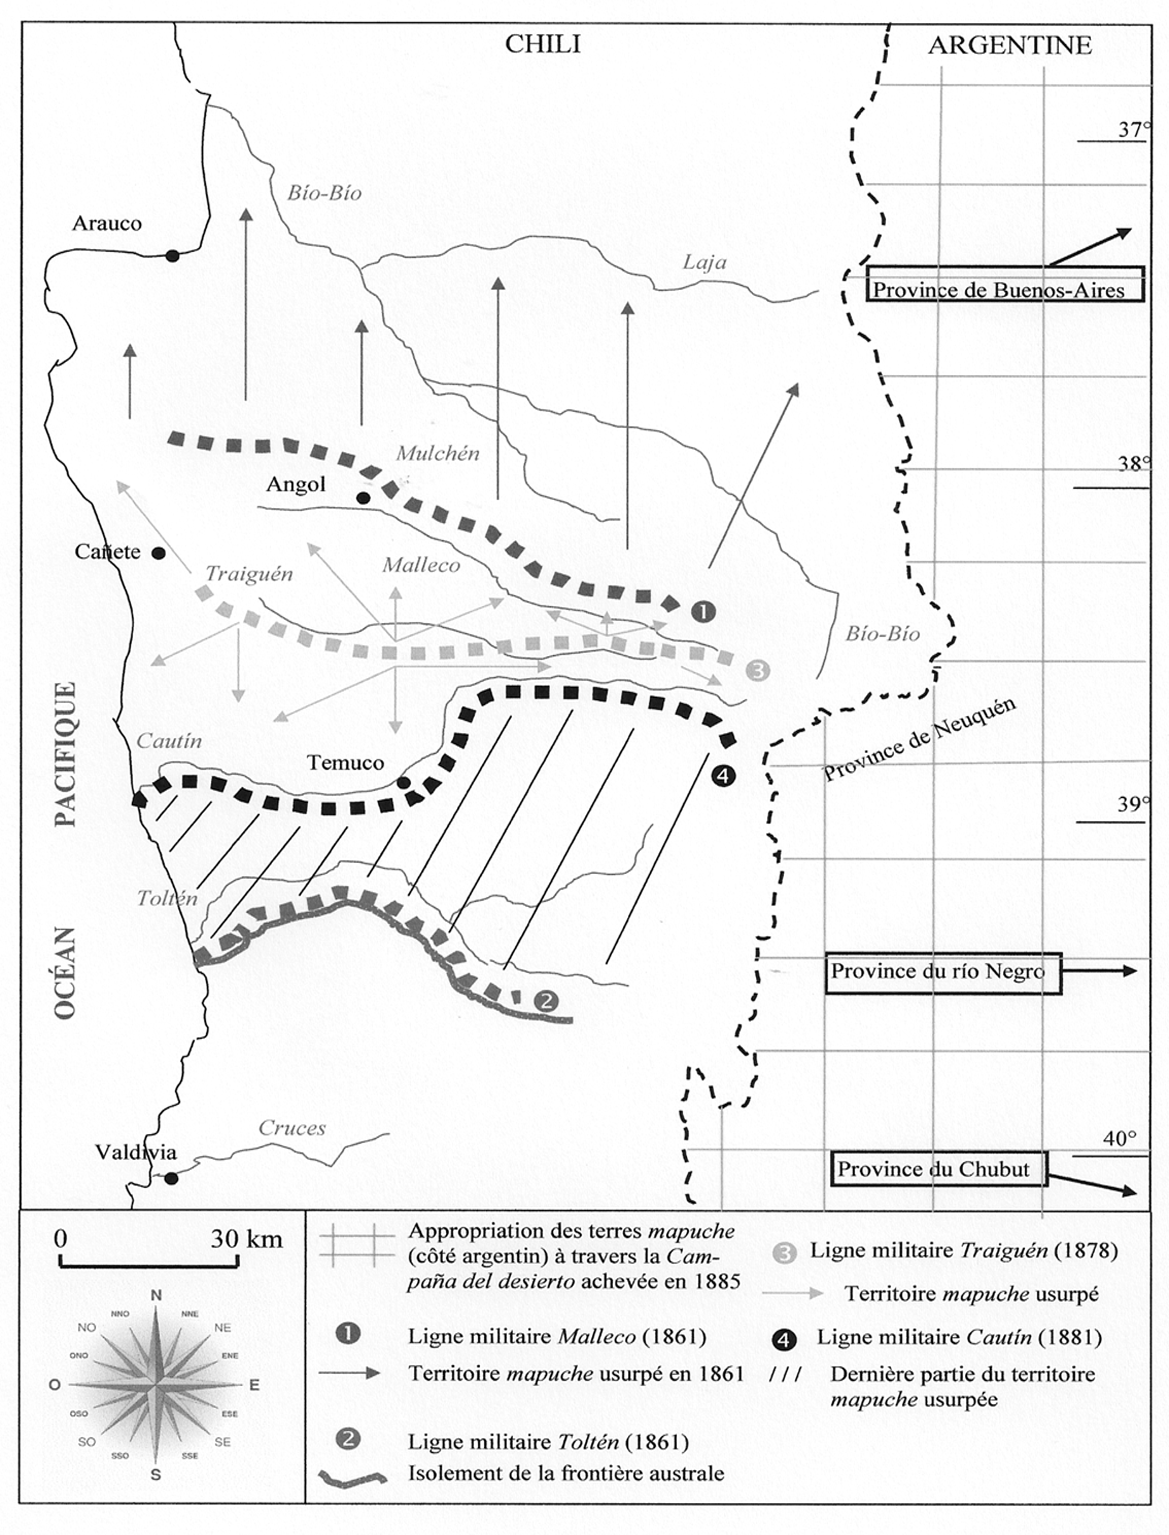
\includegraphics[width= 0.5\textwidth]{annexes/carte/carte_expansion.png}
	    \caption{Carte de l’usurpation progressive du territoire Mapuche (1810-1885)\protect\footnotemark}
	    \label{fig:my_label}
	\end{figure}
	\footnotetext{\cite{nouailleIndependanceChiliConsequences2012}}
	
	Cette répression s'intensifie à partir de 1859, après le soutien explicite de certains chefs mapuches auprès des révolutionnaires libéraux lors de l'insurrection de 1859 contre le gouvernement. En 1866, les premières lois d'occupation ont été adoptées en modifiant la nature du \enquote{territoire indigène} pour  \enquote{territoire de colonisation}. Elle entérine officiellement le processus colonial entrepris par l'État chilien avec la nomination de Cornelio Saavedra, initiateur de cette expansion, au poste d'intendant d'Arauco\footcite[p~.314]{bengoaMemoriaOlvidadaHistoria2004}. Celui-ci entama la fortification de la région tout en multipliant les lois facilitant l'appropriation des terres jusqu'au bord des rivières Malleco River et Toltén River. Durant ces 20 années, le conflit enferme progressivement le peuple Mapuche aux confins des terres araucaniennes et de la Cordillère des Andes, perdant ainsi 90,7\% de son territoire original\footcite[p~.350]{bengoaMemoriaOlvidadaHistoria2004}.
	
	Le conflit autour de l'Occupation de l'Araucanie qui dura jusqu'en 1881, n'est pas un épiphénomène au sein d'un processus d'extension territoriale et d'affirmation politique. Il est un tournant progressif majeur en enterrant définitivement une identité fondée sur un État-nation pluriel, comme nous l'évoque l'historien Pablo Mariman Quemenado: 
	
	\begin{quote}
	    \enquote{Il s'est terminé l'idée d'un État qui abhorre la diversité qui le constitue, fondant la relation et la situation coloniales avec des peuples désormais catégorisés comme "communautés indigènes"\footnote{\enquote{Concluida esta, se termina consumando la idea de un  Estado  que  abomina  de  la  diversidad  que  lo  constituye,  fundando  la  relación  y  situación  colonial  con  pueblos  que  fueron  categorizados  en  adelante  como  “comunidades indígenas”}\cite{quemenadoGeoestrategiaConflictoChileno2017a}}}
	\end{quote}
	
	\begin{figure}[p]
	    \centering
	    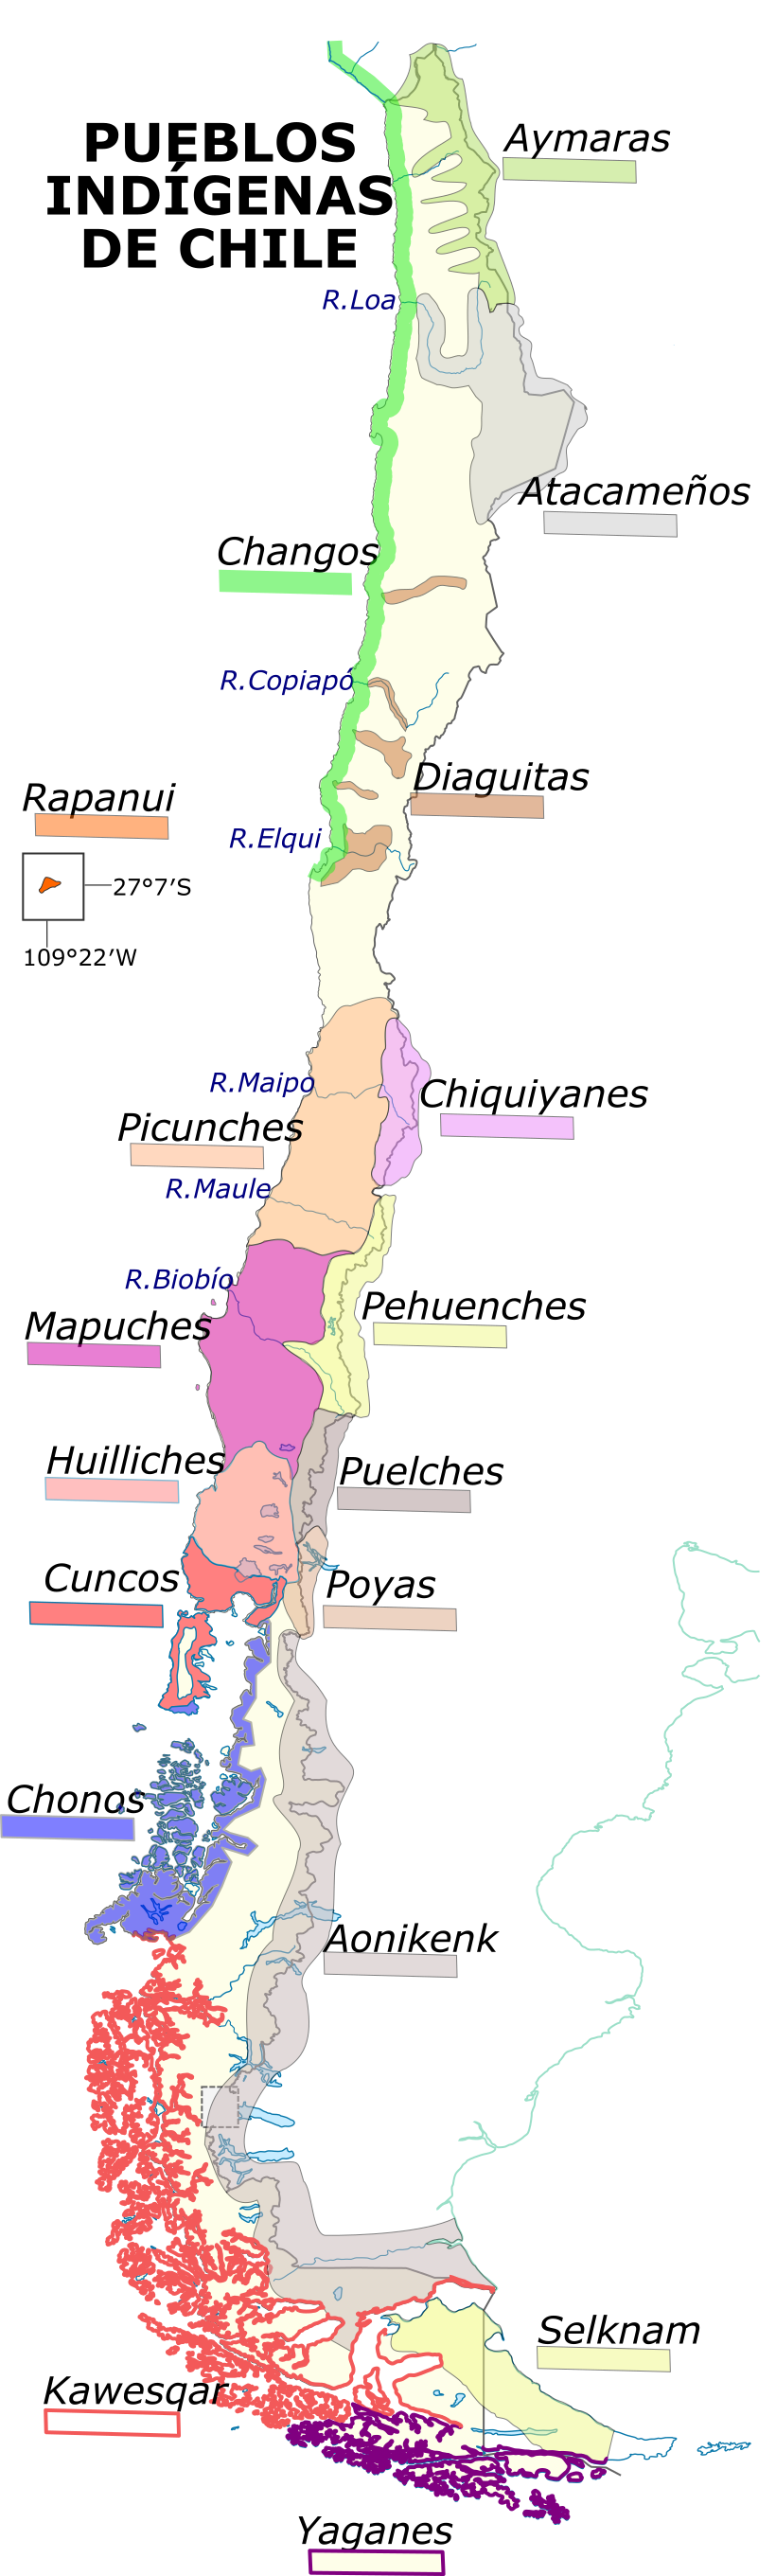
\includegraphics[width= 0.45\textwidth]{annexes/carte/carte_peuples.png}
	    \caption{Carte schématique des principaux peuples autochtones existants ou ayant existés au sein du territoire chilien actuel - \copyright Wikipedia}
	    \label{fig:carte_chili}
	\end{figure}
	
	\subsection{La question Mapuche : symbole des problèmes socio-politiques du Chili contemporain}
	
	À l'heure actuelle, la lutte pour la légitimité des droits territoriaux et politiques Mapuche est devenue un symbole de mobilisation ethno-sociale à la fois sur le plan national qu'international. Sa lutte singulière s’est progressivement transformée en une source d’inspiration culturelle inaltérable et presque romantique face à l'étatisme et la capitalisme néo-libéral\footcite{sepulvedaPaysMapucheTerritoire2012}.
	
	Dès 1910, un premier mouvement autochtone Mapuche se forme à travers le collectif \textit{Sociedad Caupolican de Defensa de la Araucanía}. Au cours du XX\textsuperscript{e} siècle, de nombreuses organisations politiques voient le jours avant de disparaître selon les tournants de l'histoire politique chilienne. Ce conflit latent accompagne au contraire le débat et les querelles sur fond d'inimitié ou au contraire de solidarité. Cette réclamation territoriale est devenue multiple et s'étend jusqu'aux territoires argentins, là où la culture et l'influence Mapuche demeure : \enquote{en renouant avec les connexions transandines de l’époque coloniale, le déploiement des systèmes circulatoires contemporains à l’échelle du cône sud-américain redonne une indéniable matérialité\footcite{sepulvedaPaysMapucheTerritoire2012}}.
	
	Si des territoires exclusifs et protégés ont été déterminés afin de reconnaître certains droits aux peuples indigènes présents sur le territoire chilien. Cette rédemption hésitante reste constamment sous le feu des critiques politiques et économiques. Aujourd'hui, si l'appartenance ethnique et les traditions culturelles se perpétuent, cette population est confrontée à de nombreux problèmes socio-économiques représentant environ un million de personnes\footcite{bengoaMapuchesHistoriaCultura2011}. En effet, la plupart des territoire hors réserves indigènes, restent soumis au monopole d'une grande industrie forestière, agricole et piscicole réfractaire face à la perte de leurs capitaux\footcite{andradeLuchaPorTerritorio2019}. Cette dépossession économique alimente les conflits locaux , mais aussi nationaux.
	
	Ces crispations sociales se sont exacerbées à partir des années 1990, où l'utilisation de la violence politique comme une pratique de contestation connaît un léger regain suite à la fébrilité de la loi Indigène de 1993. Au sein des sphères politiques et médiatiques se dresse progressivement une criminalisation de la lutte politique mapuche, dépeignant son intensification comme une menace contre l'État\footcite{carvajal-delmarCriminalisationConflitMapuche2014}. Sous fond d'une politique de discrimination raciale, la politique répressive de la contestation va être étendue par l'emploi de la loi antiterroriste promulguée en 1984 sous de la dictature de Pinochet\footcite{carvajal-delmarCriminalisationConflitMapuche2014}. 
	
	Depuis le début des années 2000, l'État chilien prétend mettre fin avec cette politique répressive des contestations avec un peuple chilien qui souhaite démontrer une plus large volonté de conciliation\footcite{nouailleIndependanceChiliConsequences2012}. Néanmoins, les tensions localisées persistent dans la région de Biobío et de l'Araucanie. Certains territoires de la région de Wallmapu sont encore récemment soumis à un état d'exception juridique et une militarisation de la région. Ces tensions encore très vives démontrent la continuité d'un conflit historique dont les enjeux sociaux et politiques persistent.
	    
    \subsection{La sous-collection de l'\textit{Araucania}}
    
    La "Colección Manuscritos" est l'un des fonds les plus importants détenus par le centre \gls{acab}, avec plus de 2200 documents manuscrits datant de 1642 à 1952. Cette collection s'est progressivement constituée grâce à des dons d'universitaires et de politiciens liés à l'Universidad de Chile, mais aussi grâce à diverses acquisitions au cours du XX\textsuperscript{e} siècle\footnote{Voir le registre de l'inventaire de "Colección Manuscritos", \textit{Archivo Central Andrés Bello}, url: \url{http://archivobello.uchile.cl/content/Registro\%20Guia/2016/enero/registro_guia_coleccion_manuscritos.pdf}, consulté le 02/08/2022.}. Ces documents se regroupent autour de différentes grandes thématiques de l'histoire du Chili et dont une grande partie a été produite par des figures éminentes de la vie politique, militaire et intellectuelle (Andres Bello, Manuel Montt, etc.). De par le prestige de ses producteurs et de l'importance historique de ces documents, ce fonds a été classé comme \enquote{Monument historique} par le décret n°295-2009 du ministère de l'Éducation du Chili durant l'année 2009\footnote{Décret n°295-2009 du ministère de l'Éducation du Chili, \textit{Declara Monumento Nacional en la categoría de Monumento Histórico las colecciones Neruda, Americana y Manuscritos, pertenecientes al Archivo Central Andrés Bello, de la Universidad de Chile}, promulgé le 5 août 2009 et publié le 5 septembre 2009}.\newpar
    
    Les archives concernant l'Occupation de l'Araucanie en constituent une part essentielle. Ce sous-fonds spécifique autour des archives de l'Occupation de l'Araucanie a été inventorié partiellement à partir de la fin des années 2000, dans le prolongement de la création de la collection "Colección Manuscritos". Cette première classification et la restauration parcellaire et progressive à permis de mettre à jours des centaines d'archives, suscitant l'intérêt des milieux scientifiques et patrimoniaux. 
    
    En 2013, un important  travail de numérisation a été mis en place, axée sur la pacification de l'Araucanie, grâce à l'octroi d'un fonds du programme ADAI (Apoyo al Desarrollo de los Archivos Iberoamericanos) qui permettra la numérisation de 249 documents, pour un total de 530 pages. Ce programme a permis de donner suite à une première transcription manuelle les années suivantes. Ce projet d'édition numérique s'inscrit donc dans cette continuité en s'appuyant sur les différents travaux précédents.\newpar
    
    En observant plus en détail, les archives numérisées du sous-fonds de la "Colección Manuscritos", nous pouvons remarquer que l'essentiel de l'activité de la production documentaire se concentre sur la période 1859-1860. Cette période de transition se situe plus exactement entre la fin des \enquote{guerras civiles "montistas"} (1850-1859) dont l'année 1859 est marquée par le soulèvement général de nombreuse tribut mapuche. Cette répression fut suivi d'une campagne de militarisation et pacification de la région dirigée par Nicolas Saavedra. Il mit ensuite en œuvre du plan d'occupation de la région Biobío à partir de 1861\footcite[p.~165-171]{bengoaHistoriaPuebloMapuche1987}. Le recensement de l'activité se concentre surtout la fin de l'année 1859 à février 1860, avec un certain regain pour le mois de juin et octobre 1860 (voir annexe A, figure \ref{fig:day_activities}). Toutefois, on retrouve de nombreux documents s'éparpillant sur l'ensemble de la seconde moitié du XIX\textsuperscript{e} siècle, bien qu'une part essentielle n'est pas encore pu être numérisé.


	\section{La construction d'un jeu de donnée : vers une utilisation tout terrain}
	\sectionmark{La construction d'un jeu de donnée}
	
	\subsection{Préparation des données numérisées et leur inventorisation}
	
	La constitution d'un jeu de données homogène et structuré a été une étape importante dans la préparation, à la fois pour s'immerger et comprendre les informations et les subtilités qui en résident. Comme nous l'avons vu précédemment, ce corpus documentaire autour des archives de l' \enquote{Occupation de l'Araucanie} a déjà été le fruit d'un long travail de révision et d'inventorisation minutieux de la part de l'équipe en charge du processus d'archivage. L'ensemble des informations ont été recueilli sous la forme d'un tableur Excel (Word office) en rassemblant des données sur chaque pièce de ce fonds partiel : date, côtes et identifiant des numérisations, indications géographiques et humaines, type, nombre.
	
	Toutefois, un certain nombre d'éléments ne furent pas adaptés à une exploitation machine, mais davantage à une interprétation humaine. Un travail de réconciliation, d'uniformisation et d'épuration des données a été mis en place en extrayant les données sous le format \gls{csv}. Ce format fut ainsi interprétable par le logiciel \texttt{Dataiku DSS}. Cette plateforme de développement intégré est destinée à l'ensemble des besoins dans le cadre traitement et analyse de la donnée. \texttt{Dataiku} a ainsi permis le retypages des données initiales, mais aussi de quantifier les archives numérisées\footnote{L'ensemble du flux de travail est disponible à l'adresse suivante : \url{https://github.com/Proyecto-Ocupacion-Araucania-UChile/Data_preparation}.}. Les enjeux de ce traitement se déclinent en trois objectifs: \\
	\begin{itemize}
	    \item Inventaire des fichiers permettant de vérifier si certains fichiers ne sont pas manquants. Il fut ensuite possible de les classer en fonction de la nature et la typologie des documents.
	    \item La conversion des images. À l'origine, le service de numérisation de \gls{acab} a produit les images sous le format \gls{tiff} (à 1200 dpi) permettant une qualité maximale. C'est un format d'image matricielle permettant de ne pas compresser l'image et ainsi de garder celle-ci la plus authentique possible en limitant la perte des données. Ce standard au sein des institutions patrimoniales reste en revanche un objet extrêmement lourd avec une moyenne autour de 60 mo (mégaoctets). Des projets similaires ont démontré qu'une telle qualité n'était pas nécessaire et qu'une image compressée est amplement suffisant\footcite{n.c.ExperimentationsLECTAUREP, chiffoleauDAHNProjectDigital2022}. Ce script shell a permis d'automatiser la conversion de l'ensemble des images vers le format \gls{jpg} \footnote{voir annexe \ref{code:shell_img}.}.
        \item Faciliter l'interprétation des données dans un travail d'analyse ou comme support à la production de métadonnées lors de son édition. \\
	\end{itemize}
	
	Cette première étape permet de mettre en place une stratégie, évolutive néanmoins quant à la constitution du set de données mais aussi sur la mise en place de certains stratagèmes afin de récupérer la donnée le plus efficacement possible avec une perte marginale. Notre jeu de données disponibles est en effet assez restreint au vue de certains autres projets de reconnaissance d'écritures manuscrites; il est donc impératif de maximiser celle-ci. Il faut pour cela essayer de sélectionner les plus qualitatives, représentatives et homogènes possibles. En observant les différents graphiques, on peut apercevoir la sur-représentation des lettres, et secondairement les notes manuscrites au sein du corpus documentaire (graphique \ref{fig:percent_type}). Nous avons donc pris la décision de centraliser les efforts sur ces deux typologies, avant d'étendre le processus en fonction du résultat. Dans un deuxième temps, la distribution des archives montrent une grande pluralité d'auteurs au sein de ce fonds. En revanche, six personnes se manifestent comme amplement plus prolifiques que la moyenne (graphique \ref{fig:author_distribution}).
	
	\subsection{Constitution d'un corpus interopérable}
	
	À la suite de différentes recherches sur l'existence de \textit{dataset}, il est rapidement apparu que la langue espagnole occupait une position plus marginale dans les domaines de la recherche et de l'ingénierie autour de l'\gls{htr}. Si quelques projets ont été mis en place, l'essentiel se tourne vers la recherche fondamentale sur les réseaux neuronaux ou ne sont pas librement accessibles\footnote{À cet égard, on peut remarquer que l'\textit{Universitat Politècnica de València} est particulièrement actif à ce sujet comme le démontre les récentes publications : \cite{granellTranscriptionSpanishHistorical2018, espana-boqueraSpanishDatasetReproducible2022}}. De la même manière, des plateformes telles que \texttt{HTR-United} ne recensent que très peu de données disponibles sur cette langue, ou alors inadaptées à la construction d'un modèle adapté \gls{acab}.
	
	Face à ces premiers constats, l'édification d'un modèle dédié paraît donc indispensable, ce qui nécessite de construire au préalable un lot de données d'entraînement. Le premier enjeu de cette automatisation est en réalité triple puisqu'il s'agît d'établir les règles structurelles, épistémologiques et analytiques des transcriptions et de l'interprétation machine. La qualité des données utilisées et leur cohérence sont à la source du succès des prédictions, dans le cadre d'un apprentissage machine supervisée\footnote{Cf. chapitre 4}.
	
	En effet, des erreurs d’acquisition ou de transformation liées à des fautes humaines ou techniques peuvent considérablement ralentir, voire mettre à mal la poursuite du projet. La performance de cette chaîne de traitement, mais aussi la réutilisation à moindre coût énergétique et de temps va dépendre d'une analyse préalable des sources. La dimension d'interopérabilité doit permettre l'utilisation multiple de ce jeu de donnée sur l'ensemble du processus de traitement : segmentation, reconnaissance d'écriture manuscrite et reconnaissance d'entités nommées. \newpar
	
	La constitution d'un corpus documentaire dans le but de l'exploiter dans un projet d'édition numérique, nécessite donc un set quantitatif, mais surtout qualitatif afin de procéder à une restitution de l'information la plus complète possible. Si l'aspect quantitatif semble de prime abord plus que négligeable en comparaison d'autres projets, plusieurs études ont démontré l'efficacité de jeu de données à la taille plus modeste tout en permettant un coût marginal\footcite{sanchezSetBenchmarksHandwritten2019}. La principale difficulté réside dans la segmentation et non la reconnaissance de caractères. Par la suite, les chercheurs Phillip Benjamin Strobel, Simon Clematide et Martin Volk ont démontré qu'un jeu de données de plus de 50 pages était suffisant pour avoir des prédictions pouvant être qualifiées de bonnes sur le moteur \gls{kraken} \footcite{strobelHowMuchData2020}.
	
	Au vu de nos précédentes analyses, il est frappant de voir la forte hétérogénéité de notre corpus ce qui induit la nécessité d'un modèle polyvalent en conséquence d'un fonds extrêmement composite. 
	Ces données préliminaires vont ainsi révéler un ensemble de facteurs et problématiques à prendre en compte afin de tendre vers une automatisation la plus efficiente possible\footcite{chagueDeuxSieclesSources2019a}.
	

    \begin{table}[h!]
    \centering
    \begin{adjustbox}{max width=1\textwidth}
    \begin{tabular}{|c|c|ccc}
    \hline
    \multicolumn{1}{|l|}{\textbf{Nom}} & \multicolumn{1}{l|}{\textbf{Pages}} & \multicolumn{1}{l|}{\textbf{Dates extrêmes}}       & \multicolumn{1}{l|}{\textbf{Particularités}}                                                         & \multicolumn{1}{l|}{\textbf{Données test}} \\ \hline
    Cornelio, Saavedra                 & 43                                              & \multicolumn{1}{c|}{nov. 1859 - août 1877}     & \multicolumn{1}{c|}{style propre, bon état, présence de notes post-scriptum}                         & \multicolumn{1}{c|}{Non}                   \\ \hline
    Avello, Juan                       & 12                                              & \multicolumn{1}{c|}{nov. 1859 - nov. 1860} & \multicolumn{1}{c|}{style propre, quelques feuilles abimées, présence de notes post-scriptum}        & \multicolumn{1}{c|}{Non}                   \\ \hline
    Díaz, José Del Carmen              & 21                                              & \multicolumn{1}{c|}{déc. 1859 - mars 1860}     & \multicolumn{1}{c|}{style propre parfois condensé, bon état}                                         & \multicolumn{1}{c|}{Non}                   \\ \hline
    Escala, Manuel Segundo             & 13                                              & \multicolumn{1}{c|}{nov. 1859 - nov. 1860} & \multicolumn{1}{c|}{style très propre, bon état}                                                     & \multicolumn{1}{c|}{Non}                   \\ \hline
    García Videla, Daniel              & 8                                               & \multicolumn{1}{c|}{mai 1860 - juin 1860}          & \multicolumn{1}{c|}{style très propre, bon état}                                                     & \multicolumn{1}{c|}{Non}                   \\ \hline
    Pérez Rosales, Vicente             & 12                                              & \multicolumn{1}{c|}{fév. 1860 - nov. 1860}  & \multicolumn{1}{c|}{style parfois hésitant et condensé, bon état}                                    & \multicolumn{1}{c|}{Non}                   \\ \hline
    Sepúlveda, José                    & 8                                               & \multicolumn{1}{c|}{déc. 1859 -nov. 1860}  & \multicolumn{1}{c|}{style intermédiaire, quelques feuilles abimées, présence de notes post-scriptum} & \multicolumn{1}{c|}{Oui}                   \\ \hline
    Villalón, Vicente                  & 22                                              & \multicolumn{1}{c|}{nov. 1859 - nov. 1859} & \multicolumn{1}{c|}{style propre, parfois effacé, présence de notes post-scriptum}                   & \multicolumn{1}{c|}{Non}                   \\ \hline
    Contreras, Juan                    & 16                                              & \multicolumn{1}{c|}{mars 1860 - juin 1860}         & \multicolumn{1}{c|}{style convenable, quelques feuilles légèrement abimées}                          & \multicolumn{1}{c|}{Non}                   \\ \hline
    Echantillon composite              & 25                                              & \multicolumn{1}{c|}{nov. 1859 - nov. 1859} & \multicolumn{1}{c|}{16 mains, bon état}                                                              & \multicolumn{1}{c|}{Non}                  \\ \hline
    \multicolumn{1}{|l|}{TOTAL}        & \multicolumn{1}{l|}{180}                        & \multicolumn{3}{l}{\cellcolor[HTML]{C0C0C0}{\color[HTML]{9B9B9B} }}                                                                                                                                    \\ \cline{1-2}
    \end{tabular}
    \end{adjustbox}
    \caption{Détails du jeu de données sélectionné}
    \label{tab:dataset}
    \end{table}

	
	Cet échantillonnage a été réalisé, de manière progressive et empirique, à partir de multiples mains en en s'appuyant sur le schéma du projet \enquote{LECTAUREP\footnote{\textit{LECTure Automatique de REPertoire}; pour plus d'informations, voir \url{https://lectaurep.hypotheses.org/}.}} mis en place par l'équipe ALMAnaCH de l'\gls{inria}. En premier lieu, le corpus s'est construit autour de plusieurs lots alternant entre 10 et 15 numérisations par auteur au nombre 6. Petit à petit, d'autres transcriptions ont été agrégées au lot déjà existant. À partir de là, la stratégie d'apprentissage s'est appuyée sur un lot conséquent d'une main unique (plus de 40 documents), un nombre de mains variables avec une production documentaire modérée voire élevée et un lot s'appuyant sur de très courtes transcriptions venant de nombreuses mains différentes. Ce choix vise à permettre un apprentissage stylistique et graphologique extrêmement varié et ainsi permettre la production d'un modèle le plus polyvalent possible en s'appuyant sur une méthodologie dite générique \footcite{pincheCREMMALabProjectHandwritten2022}.
	
	\section{Disséquer l'image et reconstruire l'information : une étape préliminaire à la transformation éditoriale}
	\sectionmark{Disséquer l'image et reconstruire l'information}
	
	La segmentation est un principe général du traitement et de l'analyse optique d’une image afin d’obtenir la reconnaissance des régions et des lignes d’écriture. De nombreux projets d'éditions numériques s'appuient justement sur cette reconnaissance pour transformer une image brute en édition numérique native.
	La mise en place de ce procédé nécessite au préalable une clarification des enjeux sémantiques et  en définissant au préalable un protocole d'annotation et de transcription. L'emploi d'une telle méthode doit ainsi permettre une automatisation de l'extraction de l'information dans son contexte, s'apparentant à une analyse diplomatique, et vérifier la solidité du processus de transformation.
	
	\subsection{Ontologie d'une procédure de segmentation d'un document}
	
	Comme nous pourrons l'observer plus en détail au sein du chapitre 4, l'un des principes novateurs de l'\gls{htr} est l'analyse de la mise en page (\textit{layout analysis}) dans le processus de reconnaissance des écritures. Cette étape consiste à détecter les zones d’intérêts dans une image, les différencier et spécifier leur intérêt : ligne de texte, régions, réclames, marges. On déconcentre le processus d'apprentissage\footcite[p.~25]{noemieOCRHTRGraphie2022}. C'est-à-dire que l'écriture n'est plus l'unique point de fixation, c'est désormais l'ensemble de la page qui est prise en compte pour en attraper l'information substantielle.
	
	Cette technologie dans le domaine de la reconnaissance d'écriture offre ainsi un double avantage : la reconnaissance d'écriture manuscrite complexe et une reconnaissance morphologique de l'image au travers de son processus de segmentation. Ces régions et ses bases de lignes vont permettre de recontextualiser le texte au moyen d'une structuration sémantique de la donnée. L'intérêt est de conserver la structure diplomatique initiale en vue de l'encodage éditorial du texte. 
	
	\begin{figure}[h!]
	    \centering
	    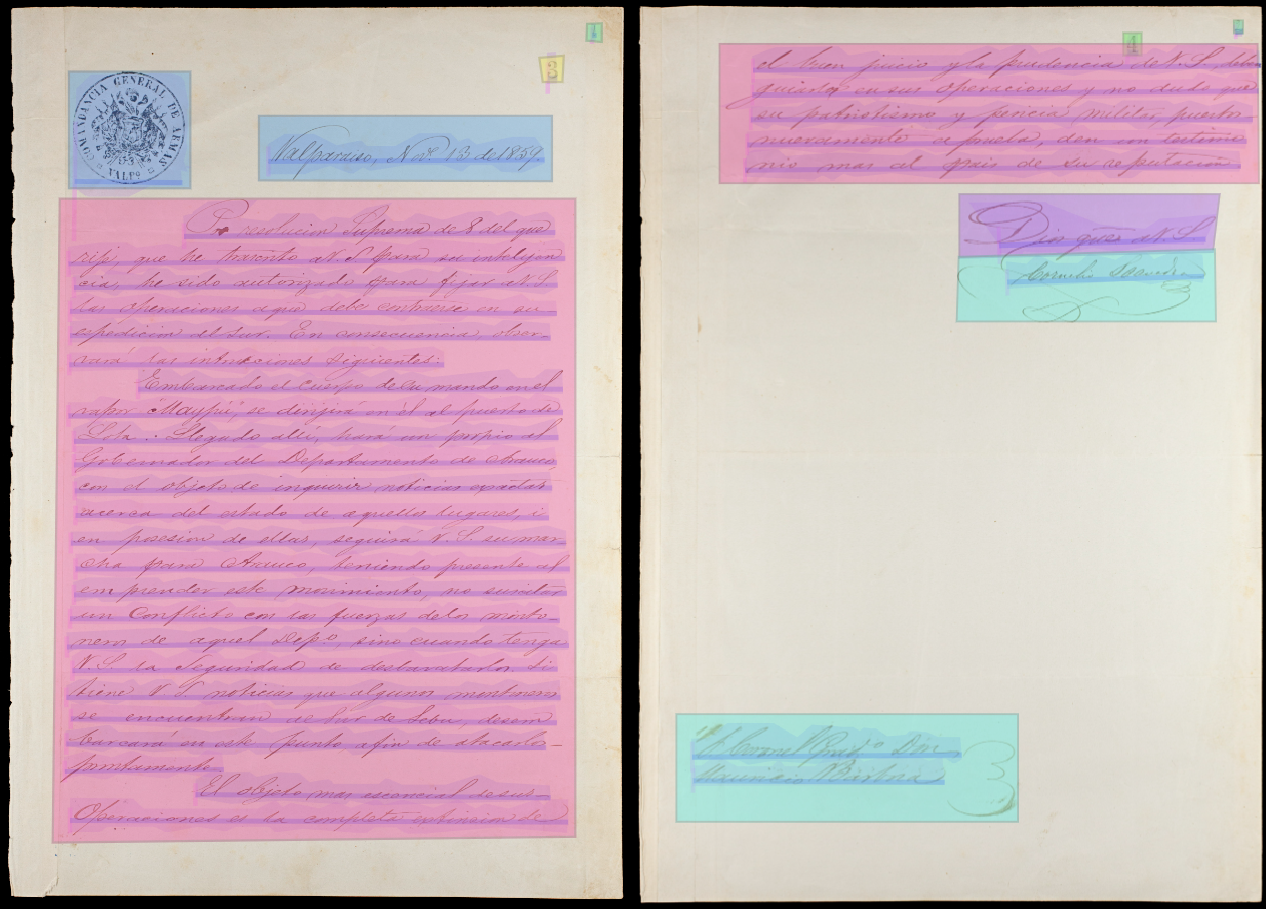
\includegraphics[width = 0.90\textwidth]{annexes/img/segmentation_img.png}
	    \caption{Démonstration d'une segmentation d'image sur l'application \gls{eScriptorium}}
	    \label{fig:segmentation}
	\end{figure}
	
	Comme nous pouvons le constater à travers de cette image reprenant la codification des régions, la stratégie adoptée s'est appuyée sur une délimitation sémantique, au détriment de la segmentation centrée sur une perception visuelle (voir figure \ref{fig:segmentation}). Si cette méthode permet de conserver au maximum le sens de la donnée initiale, elle se fait au détriment d'une cohérence visuelle. On peut observer que de nombreuses lignes sont régulièrement rapprochées entre elles, voir superposées. Cette structuration graphique peut donner lieu à un certain nombre de confusions lors du processus de segmentation machine.
	
	D'autres projets d'édition numérique ont eu pour enjeux la structuration de données autour de nature similaire à celui du projet du centre \gls{acab}. Les travaux de Floriane Chiffoleau et Anne Baillot sur le projet de \gls{dahn} ont ainsi pu expérimenter l'élaboration d'une ontologie des corpus littéraires et mettre à disposition des \textit{guidelines} décrivant les principes généraux\footcite{chiffoleauDAHNProjectDigital2022}. Sur ce constat et en s'appuyant sur une première appréciation du corpus documentaire, une ontologie a pu être dessinée dans le but d'annoter les différentes régions et les différentes lignes détectées . Celle-ci se décline sur 14 types de régions et 3 types de lignes présentées ci-dessous: \\
	
	\begin{itemize}
	    \item \textbf{Régions} :
	    \begin{enumerate}
	        \item \textit{CustomZone:Address} -- Zone indiquant le destinataire
	        \item \textit{CustomZone:Dateline} -- Zone indiquant le contexte d'écriture (date et lieu)
	        \item \textit{CustomZone:Object} -- Zone indiquant l'objet du document
	        \item \textit{MainZone:SaluteConclude} -- Zone indiquant la salutation conclusive
	        \item \textit{MainZone:SaluteIntro} -- Zone indiquant la salutation introductive
	        \item \textit{MainZone:Text} -- Zone indiquant le corps du texte
	        \item \textit{MarginTextZone:commentary} -- Zone indiquant les commentaires en marge du texte
	        \item \textit{MarginTextZone:note} -- Zone indiquant les notes additionnelles
	        \item \textit{NumberingZone:id} -- Zone indiquant le numéro d'identification (\textit{a posteriori})
	        \item \textit{NumberingZone:other} -- Zone indiquant un numéro additionnel (\textit{a posteriori})
	        \item \textit{NumberingZone:page} -- Zone indiquant le numéro de page (\textit{a posteriori})
            \item \textit{QuireMarksZone:signature} -- Zone indiquant la signature de l'auteur
            \item \textit{StampZone:graphic} -- Zone indiquant une estampille graphique
            \item \textit{StampZone:manuscript} -- Zone indiquant une estampille manuscrite
	    \end{enumerate}
	    \item \textbf{Lignes} :
	    \begin{enumerate}
	        \item \textit{DefaultLine} -- Ligne par défaut
	        \item \textit{InterlinearLine:commentary} -- Ligne indiquant un commentaire entre deux lignes
	        \item \textit{InterlinearLine:correction} -- Ligne indiquant une correction entre deux lignes\newpar
	    \end{enumerate}
	\end{itemize}
	
	Cette composition doit permettre la description de trois natures de documents : les lettres, les notes et les circulaires. Si ces trois objets ont une portée sémantique différente, il en reste que cette sélection possède des caractéristiques structurelles très similaires pouvant rapidement être associées et ainsi alléger l'ontologie. Comme nous pouvons le constater, l'ontologie a été amplement enrichie au modèle initial du projet \gls{dahn}. Les particularités de notre corpus hétérogène et l'alignement sur la méthodologie de l'initiative \gls{segmonto} ont amené à reconsidérer et remodeler cette base ontologique.
	
	Avant tout créé pour parachever l'étude des manuscrits médiévaux et des imprimés anciens, le projet \gls{segmonto}, né en 2021, est une réponse de différents chercheurs aux besoins d'un modèle efficace et de faire coexister la taxonomie des numérisations et l'approche éditoriale du texte\footcite{gabaySegmOntoCommonVocabulary2021a}. Cette initiative universitaire offre un vocabulaire contrôlé permettant une description graphique d'un texte sous sa forme la plus essentielle. L'ontologie est construite autour de 15 zones principales et 6 types de lignes; auxquelles peut être additionné un complément d'information par l'utilisation des signes \enquote{:} ou \enquote{\#} en suffixe\footcite{gabaySegmOntoControlledVocabulary2021a}. En outre, l'utilisation de ce lexique renforce l'interopérabilité des données entre les projets et ainsi permettre non seulement de créer des outils numériques pérennes, mais aussi de donner la possibilité de leur réutilisation.
	
	\subsection{\texttt{XML-ALTO}: un encodage structuré adapté à l'océrisation}
	
	Afin de comprendre la portée et l'utilisation possible des données possibles, il est nécessaire de comprendre le format d'expression de celle-ci. Au sein de l'univers de la reconnaissance d'écriture, il y a deux grands standards \gls{xml} qui accompagnent principalement et structurent les résultats \gls{ocr} : le format \gls{xml} \gls{alto} et le format \gls{page}. Dans notre cas, nous avons choisi de nous appuyer sur le premier standard qui est le plus couramment utilisé, en particulier au sein des institutions patrimoniales\footcite[p.~74]{caronFormatsDonneesPour2021}. Il offre deux avantages : la conservation des données coordonnées géométriques et la superposition de l'image.
	
	Pour revenir à la base, \gls{xml} est un métalangage de structuration de données à balise publié en 1999 par le consortium \gls{w3c}. L'atout principal de ce langage est sa grande permissivité et sa grande extensibilité avec son système à chevron. \gls{alto} est un standard dérivé de \gls{xml} défini par un schéma aujourd'hui maintenu par la \textit{Library of Congress}\footcite[p.~74]{caronFormatsDonneesPour2021}. Il a été développé à partir de 2004 afin de répondre au besoin naissant de l'\gls{ocr} afin de pouvoir décrire la mise en page des documents et assurer la conservation à long terme des données. \newpar
	
	\begin{listing}
	        \begin{minted}{xml}
	        <TextBlock HPOS="842"
                   VPOS="3078"
                   WIDTH="1161"
                   HEIGHT="271"
                   ID="eSc_textblock_493a77e7"
                   TAGREFS="BT3114">
          <Shape><Polygon POINTS="883 3128 842 3342 2003 3349 1999 3078"/></Shape>
          
          
          <TextLine ID="eSc_line_1f8ebff3"
                    TAGREFS="LT1061"
                    BASELINE="1264 3203 1951 3209" 
                    HPOS="1261"
                    VPOS="3079"
                    WIDTH="690"
                    HEIGHT="156">
            <Shape><Polygon POINTS="1264 3203 1264 3140 1315 3140 1318 3140 1388 3079 1388 3079 1391 3079 1391 3079 1391 3079 1395 3079 1395 3079 1395 3079 1398 3079 1398 3079 1401 3079 1468 3095 1573 3079 1573 3079 1576 3079 1576 3079 1576 3079 1579 3079 1579 3079 1579 3079 1703 3140 1789 3111 1792 3111 1792 3111 1792 3111 1795 3111 1795 3111 1798 3111 1798 3111 1798 3111 1801 3111 1801 3111 1801 3114 1833 3143 1833 3146 1951 3146 1951 3209 1948 3235 1261 3235"/></Shape>
	    <String CONTENT="⁋J del C. Díaz"
                    HPOS="1261"
                    VPOS="3079"
                    WIDTH="690"
                    HEIGHT="156"></String>
          </TextLine>

          
        </TextBlock>
            \end{minted}
        	\caption{Structuration d'un fichier ALTO}
        	\label{code:alto_struct}
    \end{listing}
    
    Un fichier XML ALTO est composé de trois sections principales : \balise{Description} permettant de décrire les métadonnées, \balise{Styles} renseigne les données de styles (police, etc.) et \balise{Layout} est la section décrivant les différents éléments de mise en page. Dans notre cas, les deux éléments les plus intéressants sont les éléments \balise{TextBlock} et \balise{TextLine} comme nous pouvons constater à travers cet extrait du code sources d'un résultat \gls{htr} (voir le code \ref{code:alto_struct}). L'élément \balise{TextBlock} indique les différentes données liées à la région dont l'attribut \attribut{TAGREFS} affiche la référence de la région, les autres attributs sont dédiés aux informations géométriques condensées. Le sous-élément \balise{Polygon} permet de décrire le dessein du masque de la zone sur l'axe X/Y. De la même manière, \balise{TextLine} est réservé aux données autour de la ligne. Au sein du sous-élément \balise{String}, l'attribut \attribut{CONTENT} rend compte de la transcription effectuée. \newpar
    
    Récemment un certains nombres d'outils ont été mis en place afin d'appuyer la solidité des données. Dans notre cas, la jeune application HTRVX développée et promue par HTR-United a permis de vérifier le schéma des données produites, la bonne concordance entre les zones et les lignes et de valider l'utilisation du vocabulaire SegmOnto\footcite{clericeHTRUnitedHTRVXHTRVX2022}. De ce fait, il fut très facilement possible de l'intégrer au sein du \textit{workflow} \gls{github} afin de vérifier l'apport de nouvelles de données et la bonne synchronisation entre elles.
	
	\subsection{Définir un protocole de transcription et d'annotation}
	
	Au cours de la préparation de données, l'ensemble des différentes transcriptions ont été effectuées sur l'application \gls{eScriptorium} afin d'en extraire des fichiers \gls{alto} exploitables lors de nos futurs entraînements. Cette phase s'est appuyée sur la première approche de Cecilia del Carmen Ramallo Díaz et son analyse des sources autour de l'Araucanie\footcite{carmenramallodiazdelTranscripcionDocumentosSerie2014}. Néanmoins, les transcriptions des documents ont été faites à travers une modernisation de la langue. Cela reste un frein majeur qui a nécessité de s'employer à de nouvelles transcriptions littérales.
	
	Au cours de la première phase, un ensemble de stratagèmes a été mis en place afin de récupérer un maximum de particularités depuis le texte original. Il s'agit des mots soulignés, barrés ou directement corrigés, des caractères illisibles ou partiellement lisibles et enfin des lettres suscrites. L'idée initiale était de pouvoir récupérer les différentes données et leurs évolutions grâce à l'aide d'un ensemble d'\gls{regex}. Une \gls{regex}, comme son nom l'indique, est un motif de caractères permettant de capturer ou échapper un à plusieurs éléments souhaités. Elle s'appuie sur une syntaxe particulière permettant de décrire la fonctionnalité souhaitée. Par exemple, pour récupérer le contenu d'un mot barré tel que \sout{Saavedra} signalé sous la forme \verb/*Saavedra*/, cela se traduitpar le motif suivant : \verb/\*([A-Za-zÀ-ÖØ-öø-ÿ -]+)\*/.
	
	Toutefois au vu des difficultés apparentes de l'interprétation machine lors des premiers essais effectués, il a été choisi de considérablement restreindre la codification des transcriptions. Une simplification qui s'est appuyée sur la méthodologie employée par le projet \gls{lectaurep}\footcite{durandNotairesParisRepertoires2021}. Si la première des raisons s'explique par l'intention d'optimiser les résultats, l'autre facteur était de pouvoir s'aligner sur les données du projet afin de les agréger à notre corpus et donc multiplier les données utilisables. Ainsi, seulement trois règles ont été appliquées:
	
	\begin{itemize}
	    \item lettre suscrite : \^e
	    \item mot illisible : xxx
	    \item nouveau paragraphe : \P.
	\end{itemize}
	
	 Cette dernière règle a été ajoutée afin de pouvoir délimiter plus facilement les différents paragraphes lors du processus d'édition. Les différentes expériences \gls{htr} ont démontré le besoin de simplifier les différentes règles de transcriptions afin d'être le plus optimal possible. Toutefois, l'utilisation du pied-de-mouche renversé n'a pas été conservée lors de la récupération des données sous un format texte (txt)\footcite{humeauPreprocessingHTR2022}.
	 
	 \begin{figure}[h!]
	     \centering
	     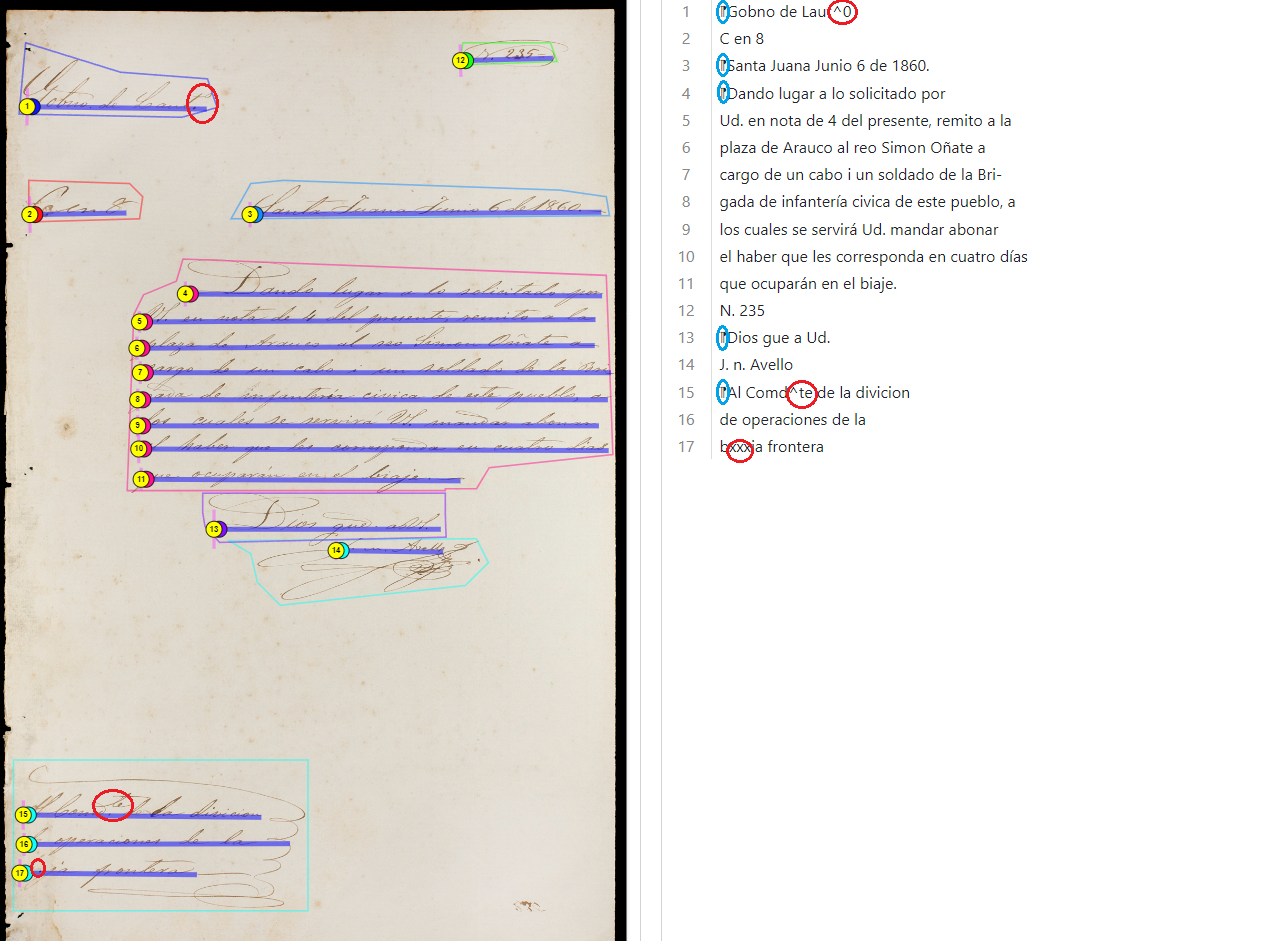
\includegraphics[width = 1.1\textwidth]{annexes/img/trans_rules.png}
	     \caption{Visualisation des règles de transcription}
	     \label{fig:transcription}
	 \end{figure}
	
	\section{Les enjeux du droit du patrimoine et de l'\textit{open data} au Chili}
	
	De nos jours, l'\textit{Open data} est devenu un enjeu majeur des institutions patrimoniales en permettant de faciliter l'accessibilité, le partage et la valorisation des données produites. Un mouvement scientifique est né autour de la volonté d'ouvrir la donnée afin de : \enquote{rendre la science plus accessible, démocratique, transparente et bénéfique pour tous\footcite{OpenScienceLatin2020}}. Une note de l'UNESCO (Organisation des Nations unies pour l'éducation, la science et la culture) révèle cet engouement général en Amérique latine afin de faire face aux problèmes d'accès aux ressources scientifiques, mais aussi à la valorisation de leur propres travaux\footcite{OpenScienceLatin2020}. 
	Toutefois, l'\textit{Open data} reste confronté à de nombreux besoins scientifiques, économiques et techniques et juridiques\footcite{jacqueminLibreAccesDonnees2019}. À travers ces observations, il s'agît de revenir sur les défis que traverse le développement d'un projet numérique autour des archives chiliennes.
	
	\subsection{Retour sur la législation des archives au Chili}
	
	En 2019, Pierre Fabry, ancien élève archiviste-paléographe, amorce quelques pistes de réflexion autour des enjeux archivistiques, sur l'accès et la transparence de l'information par rapport au mouvement de l'\textit{Estallido social} qui traverse de plein fouet l'ensemble du territoire chilien\footcite{fabryArchivesArchivistesCrise2020}. En pleine réflexion, l'insitution \textit{Archivo Nacional} émets trois problèmes majeurs auxquels le Chili doit se confronter : la mise en place d'un service d'archive électronique centralisé, le développement  des réseaux archivistiques sur l'ensemble du territoire (qui ne comprend que trois institutions publiques majeures) et surtout la mise en place d'une véritable loi sur les archives.
	
	Le développement des institutions gestionnaires des archives publiques a été considérablement mis à mal suite au coup d'État du 11 septembre 1973 et la mise en place d'un système dictatorial sous l'égide du général Pinochet (1915-2006). Une grande part des documents étatiques a été détruit durant cette période afin d'effacer les traces des exactions du régime. La transition démocratique n'a pas été l'occasion pour les différents gouvernements successifs d'avoir la volonté ni l’autorité suffisantes pour ouvrir les archives et de légiférer autour\footcite{groppoChapitreArchivesDroits2020}.
	
	Aujourd'hui, l'appareil juridique autour des archives est en réalité une législation composite regroupant un ensemble de décret et circulaires ministérielles  encadrant les institutions publiques d'archivages, notamment le centre \textit{Archivo Nacional}. Sur le plan législatif, le système des archives reste régi par la loi de 1929 dont les effets sont aujourd'hui obsolètes. Malgré la loi de 2008 sur la transparence de la vie publique, les institutions des archives condamnent les manquements persistant sur la définition des archives, de leur conservation et de leur accès. La directrice de l'époque de \textit{Archivo Nacional}, Emma de Ramón déclare : \enquote{no existe un marco legal que los ampare, proteja, reglamente y ordene\footnote{\enquote{il n'existe pas de cadre juridique pour les défendre, les protéger, les réglementer et les ordonner} in Billet de l'Universidad de Chile, \textit{Archivos en Chile: la necesidad de una ley que proteja la memoria de nuestro país}, 20 juin 2016, \url{https://www.uchile.cl/noticias/122827/archivos-en-chile-y-la-necesidad-de-una-ley-que-proteja-la-memoria-}, consulté le 5 septembre 2022.}}.
	
	Principalement, les archives restent soumises à la volonté des institutions productrices ou de conservations  qui vont définir leurs propres politiques patrimoniales. Seuls les fonds notamment classés \enquote{Monuments historiques} sont soumis à un certain nombre de restrictions avancées, prohibant notamment la destruction de documents\footnote{Ley Nº 18.845 \textit{Establece sistemas de microcopia o micrograbacion de documentos}, promulgée le 19 octobre 1989 et publiée le 3 novembre 1989}. Aujourd'hui, l'accès aux archives est un enjeu majeur de cette transition démocratique et sociale du Chili, à l'image du premier projet de constitution de l'Assemblée constituante\footnote{Le projet a finalement été refusé au cours du référendum national sur l'approbation du projet de constitution pour la République du Chili le 3 septembre 2022.}. Ce projet inscrit directement le droit d'accès aux archives au sein de la constitution, notamment avec les articles 24-5 et 162-2. Ils sont révélateurs d'une question en suspens et des besoins sociaux autour pour la transparence de la vie publique, mais aussi historique sur la question des droits indigènes et de la mémoire durant la dictature.
	
	\subsection{Libéraliser l'accès aux données numériques}
	
	La question des archives et de la production documentaire des écosystèmes électroniques a fait le fruit d'une série d'encadrements juridiques entre les années 2002 et 2004. Ils explicitent les bases des enjeux de conservations et les compétences de l'institution \textit{Archivo Nacionale} sur ce domaine, bien que rudimentaire\footcite{acevedoDocumentoElectronicoDerecho2004}. 
	
	La publication des données et la mise à disposition des données numériques des archives restent à la libre appréciation des institutions archivistiques, restreintes par le droit de la propriété intellectuelle, la législation sur les données personnelles et la loi sur la transparence des données publiques. De plus, si le producteur reste propriétaire des données, il ne possède aucun droit sur la base de données et son utilisation\footcite[p.~23]{n.c.ManualDatosAbiertos2014}. Cette situation confuse ne facilite pas la propagation de l'\textit{Open data}, qui reste souvent impopulaire auprès des instituions. Si les enjeux techniques, juridiques et politiques restent un problème certain, elle est aussi d'ordre culturelle dans un pays où la culture de la propriété reste très forte\footcite[p.~43]{n.c.EstadoArteNacional2010}.
	
	Mettre en place un projet sur les principes de la science ouverte et les principes FAIR (Trouvable, Accessible, Interopérable, Réutilisable) ne tient pas seulement au ressort des dispositions techniques. C'est aussi un travail pédagogique sur les enjeux et les bienfaits des données ouvertes pour la science et l'institution. Au contraire d'une négation du travail accompli, l'ouverture numérique est un instrument efficace pour la valorisation de celui-ci, tout en permettant de multiplier les efforts conjoints. Les licences internationales \textit{Creative Commons} sur la protection de l'utilisation des données produites sont un excellent outil de confiance pour la mise à disposition en libre accès. Dans notre cas, nous avons privilégié la licence \textit{Attribution-NonCommercial-ShareAlike 4.0 International} permettant le partage et l'utilisation des données sous condition de situation et à usage non commercial\footnote{\url{https://creativecommons.org/licenses/by-sa/4.0/}, consulté le 01/0/2022.}.
	
	Pour la mise à disposition des fichiers \gls{alto} produits, nous nous sommes appuyés sur l'initiative \textit{HTR-UNITED} qui souhaite faciliter l'accès et la réutilisation des données \gls{htr}\footnote{\textit{HTR-United}, url: \url{https://htr-united.github.io/}, consulté le 14/08/2022.}. Les différents outils mis en place tel que \texttt{HTRVX} permettent à la bonne interopérabilité entre les formats et les ontologies et ainsi vérifier la compatibilité avec ces propres données terrains. L'organisation souhaite ainsi favoriser le partage massif des données et  des modèles autour de l'\gls{htr} grâce à la standardisation des dépôts (\textit{via} \texttt{HTRUCS}), leurs recensements et faire correspondre à une charte de qualité\footcite{chagueConditionsMutualisationPrincipes2022}. Dans ce même registre, nous avons publié également les données sur la plateforme \textit{Zenodo} qui est un répertoire de travaux de recherche, de logiciel et de données.
	
	Il est clair que la mise en place d'infrastructures et d'organisations communes facilite amplement la mise à profit des données, et ce tant du point de vue technique que morale. Ces efforts communs de référencement, d'accessibilité et d'interopérabilité sont d'autant plus importants, car ils sont une opportunité de pérenniser et démocratiser les projets numériques à travers une réduction des coûts qu'ils impliquent et une circulation des savoirs\footcite{chagueConditionsMutualisationPrincipes2022}.
	
	
	
	%%%%%%%%%%%%%%% CHAPTER 2 %%%%%%%%%%%%%%% 
	
	\chapter{L'apprentissage machine et la reconnaissance de texte}
	\chaptermark{La reconnaissance de texte}
	
	Les technologies de reconnaissance d'écriture automatique s'ancrent dans une histoire longue. Elle remonte avant même la naissance de l'\gls{ia} et l'article fondateur d'Alan Turing \enquote{Computing Machinery and Intelligence}\footcite{turingComputingMachineryIntelligence1950}. C'est en 1929 que l'ingénieur allemand Gustav Tauschek développe la première technologie pouvant être affiliée au domaine de la reconnaissance manuscrite optique. Toutefois, c'est véritablement à partir des années 1960-1970 que l'\gls{ocr} connaît ses premiers résultats scientifiques satisfaisants, encourageant une première commercialisation en 1978\footcite{alkhalafOCRBasedElectronicDocumentation2014}.
	
	L'intérêt suscité pour cette technologie se fait rapidement remarquer au sein des sphères scientifiques et patrimoniales tant la reconnaissance automatique de caractères ouvre de nouvelles possibilités. Malgré des avancées prometteuses, l'\gls{ocr} est encore loin d'offrir des résultats suffisamment exploitables aussi bien du point de vue méthodologique qu'éditorial comme le relate l'historien Gian Piero Zarri\footcite{zarriQuelquesAspectsTechniques1977}. Ce fantasme de la reconnaissance des écritures par la machine ne se réalise véritablement que depuis une dizaine d'années. Durant cette décennie, on observe une multiplication de projets patrimoniaux et scientifiques autour de la reconnaissance textuelle. Hugo Scheithauer rattache cette démocratisation de la reconnaissance de texte avec le développement de la plateforme Transkribus, émergeant au début des années 2010 dans le cadre d'un financement européen\footcite{scheithauerReconnaissanceEntitesNommees2021}.
	
	À travers ces observations primaires, l'ébullition de la \gls{rem} remet profondément en question les anciennes pratiques et les anciens avis au sein du paysage scientifique et culturel. À partir du projet de l'Araucanie, nous allons observer comment la reconnaissance de texte a pu bénéficier au traitement de ces sources, mais aussi les limites atteintes de cette technologie.
	
	Ce chapitre souhaite développer les différents enjeux et les défis qu'offre l'apprentissage machine autour de l'édition numérique, notamment par le prisme de la reconnaissance des écritures. Si initialement la généralisation de l'\gls{ocr} s'exerce dans un objectif d'exploitation industrielle, l'intérêt des milieux archivistiques et patrimoniaux s'observe facilement avec la multiplication de l'impression numérique\footcite{mouffletAnsExperimentationTechnologie2021}. Les progrès exponentiels qui ont été réalisés depuis plus d'une dizaine d'années ont permis de donner un second souffle à la reconnaissance automatique de l'écriture et plus particulièrement l'écriture manuscrite. Ce renouveau favorise l'édification de projets d'envergures au sein des humanités afin de contribuer à l'extraction et l'exploitation de l'information numérique.
	
	\section{État scientifique et technique autour de la reconnaissance de texte}
	\sectionmark{État scientifique et technique}
	
	Aujourd'hui, la reconnaissance de texte est une catégorie générale se déclinant en un éventail de technologies et de techniques. On peut y distinguer deux grandes taxinomies : l'\gls{ocr} et \gls{htr} (\textit{alias} la \gls{rem}). La reconnaissance automatique de texte est une catégorie du \textit{machine learning} consistant à permettre à l'ordinateur l'interprétation de données textuelles à partir d'une image (imprimées ou manuscrites) en une suite de caractères numériques.
	
	Ce domaine de pointe se rattache ainsi à l'écosystème de l'apprentissage machine et plus particulièrement au traitement automatique de l'image (\textit{Digital image processing} en anglais), la reconnaissance de forme (\textit{Pattern recognition} en anglais) et au \gls{tal} (\textit{Natural language processing} en anglais).
	
	
	\subsection{Écriture, matrice et \textit{deep learning}}
	
	Comme nous l'avons entrevu précédemment, on distingue deux grands types au sein de la reconnaissance de texte : l'\gls{ocr} centré autour des textes imprimés et l'\gls{htr} pour les documents manuscrits. Au cours des années 1960, les premières avancées résident dans le changement ontologique de l'image en s'appuyant sur la puissance de calcul des ordinateurs. Grâce aux procédés du traitement de l'image, celle-ci est alors binarisée au travers de ses couleurs primaires ou des nuances de gris selon la méthode. C'est-à-dire que l'image est alors convertie en une suite de valeurs numériques (entiers ou décimaux) de multiples dimensions, dans ce qu'on appelle une matrice (voir figure \ref{fig:a_matrix})\footnote{Un exemple permettant de comprendre le seuillage et la binarisation est disponible. Voir annexe \ref{code:traitement_image}}. Comme le rappelle le groupe de chercheur de l'Université de Washington, les techniques de seuillage (\textit{Thresholding}) sont alors essentielles dans le processus de traitement pictural puisqu'elle permettent de segmenter l'image à partir d'une valeur booléenne, obtenant ainsi un filtrage des pixels la composant\footcite{guptaOCRBinarizationImage2007}.
	
	\begin{figure}[h]
	    \centering
	    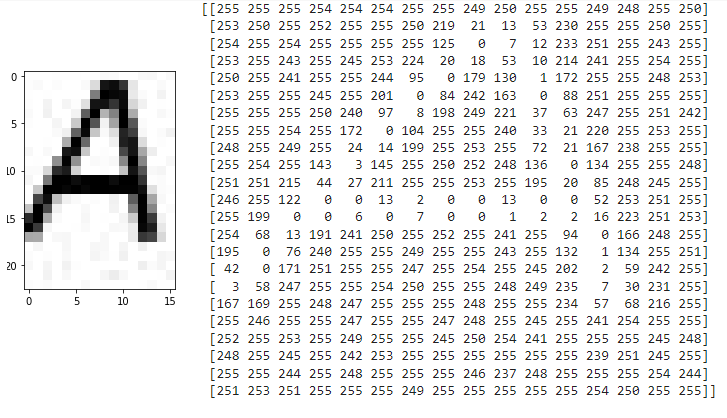
\includegraphics[width=0.7\textwidth]{annexes/img/A_to_matrix.png}
	    \caption{Transposition d'un caractère en matrice (niveau de gris)}
	    \label{fig:a_matrix}
	\end{figure}
	
	Cette transposition de l'image en une matrice décimale facilite la détermination d'un caractère \textit{via} l'application de modèles statistiques et mathématiques. L'une des premières méthodes appliquées dans le domaine de l'apprentissage machine est la méthode \textit{k-NN}(Méthode des k plus proches voisins)\footcite[p.~39]{terrielRepresenterEvaluerDonnees2020}. Pour la définir, cette technique d'apprentissage supervisée réside sur l'alignement de données étiquetées, en établissant la donnée équivalente la plus proche (la distance \textit{k}) de notre caractère x. À partir des années 1980, les laboratoires travaillant sur la reconnaissance d'écriture réutilisent les avancées dans le domaine de la linguistique et de ses modèles arithmétiques (\textit{Hidden Markov Model}) s'appuyant sur des systèmes d'occurrences et de nouveaux modèles de segmentation\footcite[p.~40]{terrielRepresenterEvaluerDonnees2020}.
	
	\subsubsection{\textit{Reconnaissance de texte et apprentissage profond}}
	
	De nos jours, les techniques de reconnaissance de texte se sont considérablement améliorées. Ce perfectionnement est dû à l’explosion du \textit{deep learning} (apprentissage profond) en 2012, suite à la victoire incontestable d'un de ces modèles lors d'un concours de classification d'images. Le procédé n'est pas nouveau puisqu'on peut remonter son origine à 1943, où le neurologue et le logicien Warren S. McCulloch et Walter Pitts décrivent une première application \enquote{neuronale} de la machine de Turing\footcite{mccullochLogicalCalculusIdeas1943}. Toutefois, la parenté de l'apprentissage profond est encore contestée puisque le chercheur Charles C. Tappert rattache davantage sa première conceptualisation à Frank Rosenblatt et son invention du perceptron\footcite[Il met en place un système probabiliste de stockage et de classifications de l'information s'appuyant sur le modèle d'un réseau neuronal][]{tappertWhoFatherDeep2019}.
	
	Le \textit{deep learning} reste en marge au sein de l'intelligence artificielle pendant de nombreuses années en raison de la puissance de calcul nécessaire à son fonctionnement intrinsèque. Malgré tout, certaines équipes de chercheurs comme celle dirigée par Yann Le Cun continuent de développer la recherche fondamentale, permettant en 2012 d'exploser les records aux yeux du monde.
	
	\begin{figure}[h!]
	    \centering
	    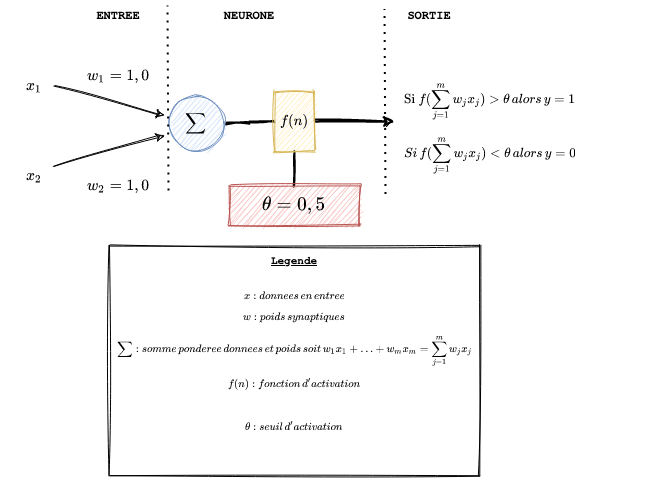
\includegraphics[width=0.9\textwidth]{annexes/graph/neurone_formel.png}
	    \caption{Illustration simplifiée d’un neurone formel, ©Lucas Terriel, 2020}
	    \label{fig:neurone}
	\end{figure}
	
	L'apprentissage profond se veut donc à la frontière de l'informatique, des mathématiques et de la neurobiologie en reprenant le modèle du neurone et du système de stimulation synaptique. Cette artificialisation numérique s'appelle le perceptron \textit{alias} le neurone simple. Pour reprendre la métaphore, le neurone reçoit une quantité d'information (les poids) dont la somme pondérée doit atteindre un certain seuil afin d'être stimulée. Cette stimulation applique une fonction d'activation ou de transfert envoyant une information de sortie (voir figure \ref{fig:neurone}). À partir de ce système, des réseaux de neurones sont alors mis en place afin de traiter des données complexes, et ce avec une spécialisation progressive. De nos jours, l'algorithme du perceptron simple est dépassé au profit de systèmes améliorés tel que le perceptron multicouche, consistant en une série de neurones simples et cachés, ou le \textit{Support Vector Machine}\footcite[Pour prolonger la curiosité, voici trois articles permettant d'expliquer certains principes généraux et des cas applicatifs:][]{nobleWhatSupportVector2006, gardnerArtificialNeuralNetworks1998, ramchounMultilayerPerceptronArchitecture2016}.
	
	À l'image de l'ensemble du domaine de l'intelligence artificielle, l'apprentissage profond a connu une véritable ébullition dans le secteur de la reconnaissance automatique de texte, et ce particulièrement après 2016\footcite{memonHandwrittenOpticalCharacter2020}. Les résultats furent rapidement très satisfaisants grâce à la capacité des réseaux de neurones à traiter des données complexes et en sa capacité de mémorisation. C'est justement sur ce dernier point que certains laboratoires ce sont appuyés pour améliorer les résultats concernant les écritures manuscrites en incitant l'utilisation d'une architecture \gls{RNN}. Cette architecture traite l'information de manière cyclique et lui permet donc de la contextualiser. Elle a rapidement affiché des taux supérieurs à 90\%, néanmoins au détriment d'une très imposante puissance de calcul\footcite{gravesOfflineHandwritingRecognition2008}. Cette architecture reste encore aujourd'hui la plus commune, même si régulièrement présente sous forme hybride. Toutefois, plusieurs groupes de chercheurs ont signalé les problèmes sous-jacents de cette architecture à la fois sur le plan technique (la distorsion et l'explosion des très grandes images) et les besoins exponentiels en terme de puissance de calcul. Les systèmes hybrides couplés avec les architectures \gls{CNN} semblent remettre en cause la suprématie des réseaux RNN en permettant une réduction considérable du coût de calcul grâce à un système de segmentation des tâches, accentué par un traitement de l'image plus important (notamment le processus d'augmentation)\footcite{puigcerverAreMultidimensionalRecurrent2017, desousanetoHTRFlorDeepLearning2020}.
	
	\subsection{La révolution technique de l'\gls{htr}}
	
	Comme nous l'avons vu précédemment, le \textit{deep learning} a consolidé amplement les nombreuses avancées dans la reconnaissance de texte et plus particulièrement le secteur de l'\gls{htr}. Dans la majorité des projets, les techniques d'apprentissage se fondent sur l'apprentissage supervisé. C'est-à-dire qu'on fournit au processus d'apprentissage des données préalablement étiquetées afin de lui fournir un support d'apprentissage à partir duquel la machine va pouvoir déployer une méthode d'analyse, et ainsi classifier les caractères.
	
	Néanmoins, la \gls{rem} n'est pas simplement due à l'essor de l'apprentissage profond, même si les avancées techniques lui sont que corrélées. En effet, l'\gls{htr} correspond à un procédé de segmentation bien spécifique en comparaison des techniques portant sur l'\gls{ocr}. Le point névralgique de cette technique de reconnaissance de texte réside dans la segmentation de l'image dans son intégralité, et non sur un centrage spécifique. À l’origine, le moteur établit un masque définissant la zone à reconnaître à partir d'une ligne de référence, souvent en bas\footcite[p.~25-26]{noemieOCRHTRGraphie2022}. Ce point d'appui permet d'exercer ce que l'on appelle la reconnaissance en-ligne ce qui signifie une conception des caractères cursifs dans l'espace et le temps par la machine. Le modèle, s'appuyant sur son expérience, va donc déchiffrer l'écriture selon ses mouvements et les comparer aux données terrain. D'autres méthodes tendent à remplacer le procédé par ligne par un système à polygone (\textit{bounding boxes}) depuis quelques années à l'image des groupes de chercheurs de l'\gls{ephe} ou de l'Université autonome de Barcelone\footcite{carbonellNeuralModelText2020, kiesslingBADAMPublicDataset2019}. Comme l'expose la figure \ref{fig:mask_baseline} s'appuyant sur le moteur kraken développé par l'\gls{ephe}, la reconnaissance des caractères s'appuie sur la détection de ligne afin de délimiter une zone de contour, un polygone permettant une meilleure détection et évaluation de l'objet\footcite[p.~26]{noemieOCRHTRGraphie2022}.
	
	\begin{figure}[h!]
	    \centering
	    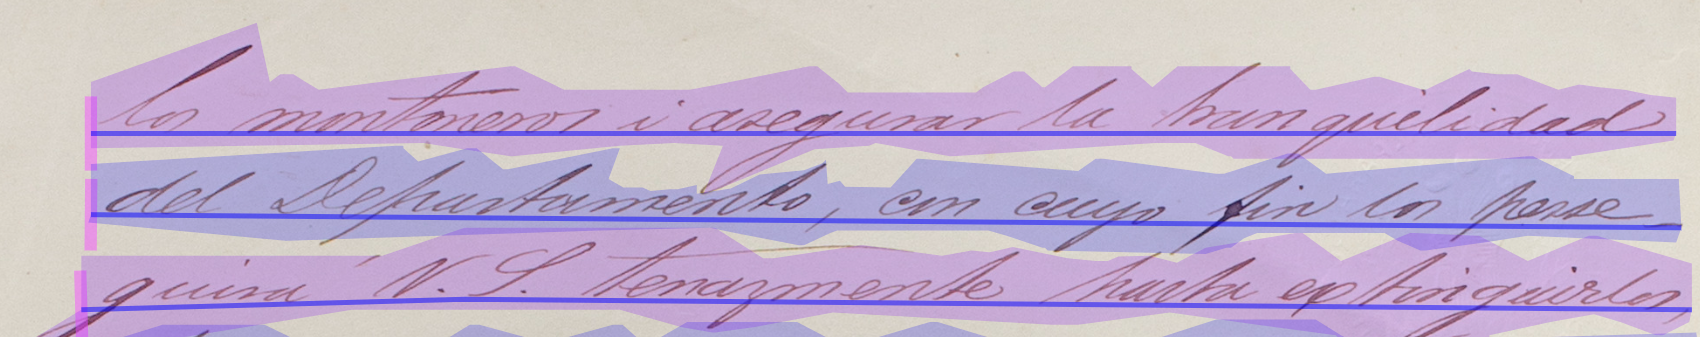
\includegraphics[width=1\textwidth]{annexes/img/mask_baseline.png}
	    \caption{Exemple de masque à partir d'une \textit{baseline}}
	    \label{fig:mask_baseline}
	\end{figure}
	
	La reconnaissance de texte n'est donc qu'une étape au sein d'un moteur \gls{htr}. Si l'on regarde le schéma suivant (figure \ref{fig:htr_schema}), on remarque trois étapes primordiales à l'obtention d'une prédiction qualitative. La détermination de cette chaîne de traitement a caractérisé de nombreux progrès au sein de la \gls{rem} et plus particulièrement au sein des écritures complexes usant de nombreux glyphes tel que l'arabe\footcite{kiesslingBADAMPublicDataset2019}. En outre, une phase de traitement des données de sorties est régulièrement ajoutée au sein des projets afin de maximiser les résultats.
	
	\begin{figure}[h!]
	    \centering
	    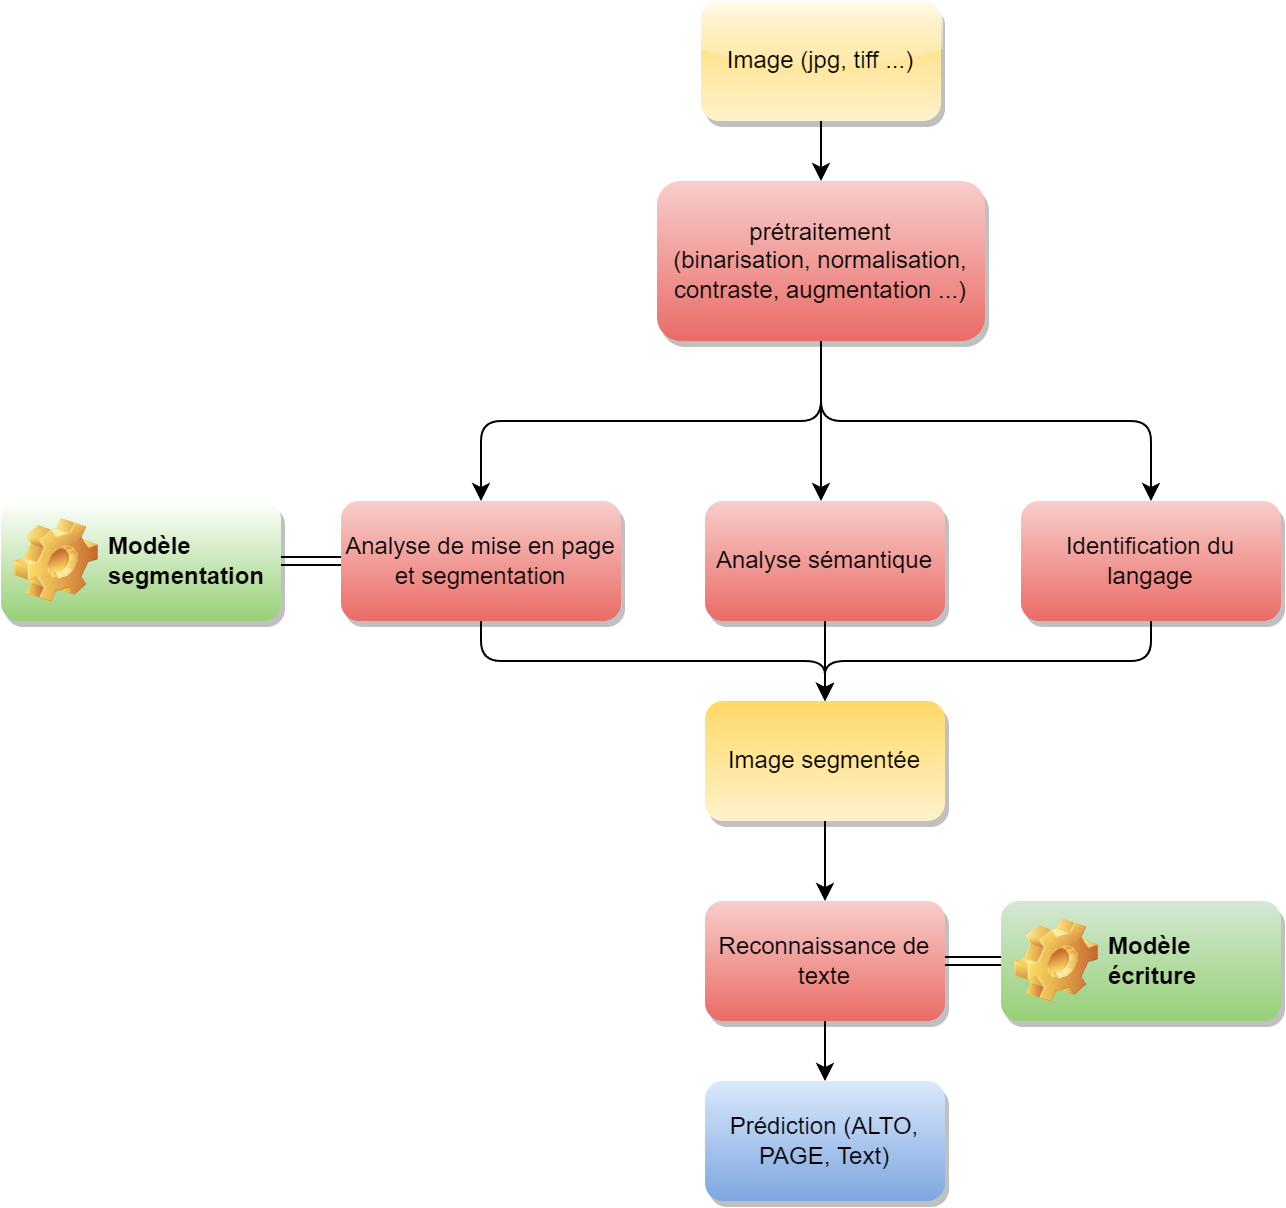
\includegraphics[width=1\textwidth]{annexes/schema/HTR_processus.png}
	    \caption{Chaîne de traitement d'un procédé \gls{htr}}
	    \label{fig:htr_schema}
	\end{figure}
	
	\subsection{\texttt{Kraken} et \texttt{eScriptorium}: moteur et application pour l'HTR}
	
	Avec l'explosion du \textit{deep learning} et de l'\gls{htr}, de nombreuses plateformes dédiées ont fait leur apparition au sein de la sphère de la \gls{rem}. Une en particulièr s'est rapidement imposée de part la qualité de ses résultats: \textit{Transkribus}, avec le financement du projet européen READ-IT(Reading Europe Advanced Investigation Tools). Elle propose des modèles extrêmement complets, permettant d'obtenir des résultats très qualitatifs. Originalement gratuite, son utilisation est devenue payante au fil du temps, tournant de nombreux projets d'édition numérique vers d'autres outils \textit{open source} tel qu'\gls{eScriptorium}.
	
	L'initiative du projet est née en 2019 par un groupe de chercheurs issus de l'institut de recherche Scripta de l'écosystème Paris Science et Lettres, et plus particulièrement de l'\gls{ephe}. Le but est de fournir une interface web de \gls{rem} à destination de l'histoire scientifique et la plus ouverte possible, en réaction à l'opacité du projet Transkribus et son nouveau modèle économique\footcite{kiesslingEScriptoriumOpenSource2019}. Le second objectif est de renforcer la \gls{rem} sur un panel de langages beaucoup plus importants grâce au soutien des compétences du laboratoire. Ce besoin naît du constat que les principaux modèles sont essentiellement adaptés aux langues latines. Scripta doit permettre d'étendre le fonctionnement de la \gls{rem} à des langues et des documents plus complexes comme le signale Peter A. Stokes:
	
	\begin{quote}
	    \enquote{It has therefore been a crucial element of the project that the software must avoid, as far as possible, all assumptions about the nature of the writing and language that is in the system. The writing may be left to right, right to left, top to bottom or even bottom to top; the support may be paper, parchment, but also stone, palm leaf, clay, wood, or many others; it may be written with a pen, painted with a brush, inscribed with a chisel; the writing system may be alphabetic, logographic, hieroglyphic; and so on.\footnote{\enquote{Un élément crucial du projet a donc été que le logiciel doit éviter, autant que possible, toute hypothèse sur la nature de l'écriture et de la langue qui se trouve dans le système. L'écriture peut être de gauche à droite, de droite à gauche, de haut en bas ou même de bas en haut ; le support peut être du papier, du parchemin, mais aussi de la pierre, de la feuille de palmier, de l'argile, du bois, ou bien d'autres encore ; elle peut être écrite à la plume, peinte au pinceau, inscrite au ciseau ; le système d'écriture peut être alphabétique, logographique, hiéroglyphique ; et ainsi de suite.} \textit{in} \cite{stokesEScriptoriumVREManuscript}}}
	\end{quote}
	
	La plateforme \gls{eScriptorium} s'appuie sur le moteur \gls{ocr} \gls{kraken} développé par Benjamin Kiessling. \gls{kraken} est un moteur clé en main interactif sous la forme d'un \gls{cli}, optimisé pour les documents historiques et les textes en caractères non latins\footcite{kiesslingKrakenUniversalText2019a}. Basé sur le moteur Ocropy, \gls{kraken} offre une très grande modularité lors de la conception de modèle de segmentation ou de reconnaissance de texte, mais aussi de multiples schémas de sortie ce qui en fait un moteur rapidement intégral au sein d'une chaîne de traitement. Le moteur est construit sur deux architectures neuronales différentes. À l’origine, le système de détection des \textit{baselines} utilise une architecture mixte \gls{CNN} et LSTM (\textit{long short-term memory}) qui est une catégorie des modèles \gls{RNN}\footcite{toselliDigitalEditionsDistant2021a}. Plusieurs études ont démontrée la capacité de cette architecture neuronale mixte à limiter le nombre de vérités terrain nécessaires à la production d'un modèle\footcite{aradillasBoostingHandwritingText2018, granetTransferLearningHandwriting2018}. Ces expérimentations architecturales et ces observations empiriques ont permises une réelle amélioration de la \gls{rem}.
	
	\begin{figure}[h!]
	    \centering
	    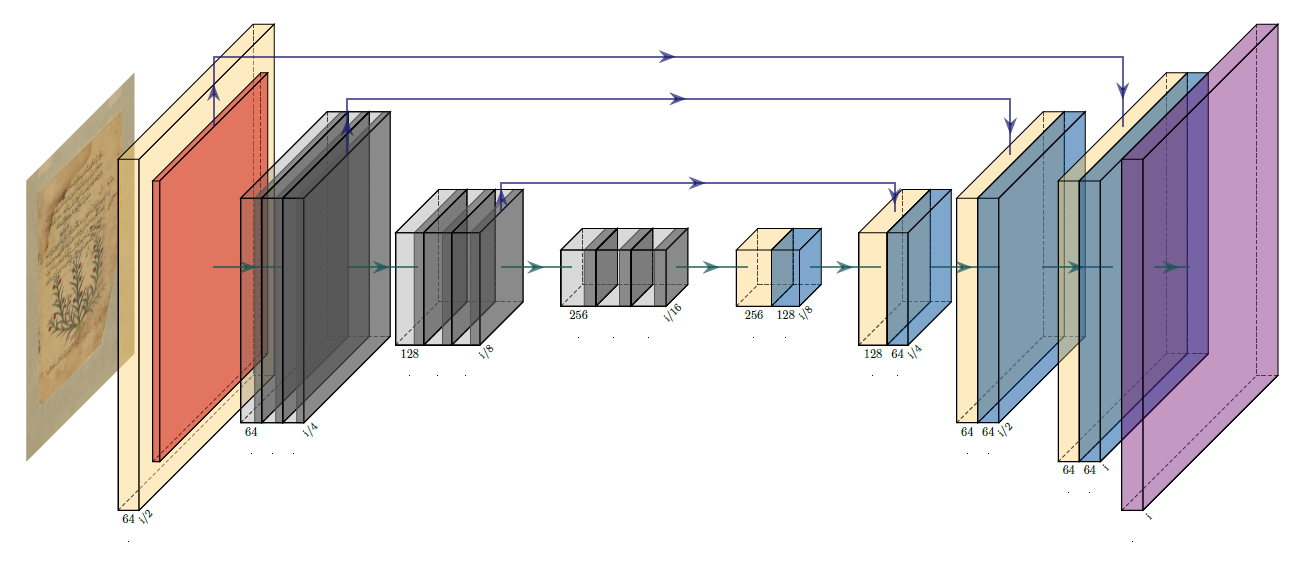
\includegraphics[width=0.8\textwidth]{annexes/schema/CNN_network.png}
	    \caption{Architecture \gls{CNN} à échantillonnage et BLSTM de détection des \textit{baselines} au sein du moteur Kraken - @Benjamin Kiessling, 2019}
	    \label{fig:cnn_archi}
	\end{figure}
	
	
	\section{Méthodologie appliquée à la production d'un modèle HTR}
	
	La plateforme \gls{eScriptorium} et le moteur \gls{kraken} ont été au centre du processus de transposition numérique des données autour des archives de l'Occupation de l'Araucania. La volonté initiale d'orienter son moteur vers le traitement des documents historiques ouvre ainsi de multiples possibilités pour la production d'une chaîne de traitement dédiée à l'édition numérique historique. En outre, le choix de procéder à une application ouverte, gratuite et modulable renforce l"accessibilité de cette technologie à des projets plus modestes et expérimentaux.
	Dans ce cadre, nous allons observer comment a été conçu à modèle \gls{rem} adapté à ces archives à partir du moteur \gls{kraken}.
	
	\subsection{Produire un modèle \gls{htr} avec \gls{kraken}}
	
	Initialement le projet souhaitait s'appuyer directement sur les ressources \textit{hardware} de la plateforme \gls{eScriptorium}, car comme nous l'avons vu le moteur \gls{kraken} nécessite une très forte puissance de calcul en raison de son architecture neuronale \gls{RNN}. Toutefois, cette puissance exigée a aussi un coût pour la structure de l'\gls{inria} et le temps d'attentes peut être assez long en fonction de la demande. Il a donc rapidement été décidé de passer par des moyens alternatifs en s'appuyant sur un \gls{gpu} personnel et d'utiliser directement le \gls{cli} \gls{kraken}.
	
	Pour la méthodologie employée, il convient de définir quelques termes complexes. Le processus d'apprentissage supervisé s'appuie sur trois types de données qui ont été préalablement compilées afin d'améliorer les performances : les données d'entraînements, les données de validation qui vont être le support d'apprentissage lors de l'entraînement et enfin les données de tests qui vont permettre d'évaluer la qualité de l'apprentissage. En général et ici dans notre cas, les données sont réparties entre 80\% pour les données d'entraînements, 10\% pour les données de validation et 10\% pour les données de tests. Chaque processus d'entraînement est nommé \textit{epoch} et se termine par la procédure d'évaluation. Lors de chaque entraînement, les données sont subdivisées en différents lots d'apprentissage simultané (\textit{batch}) permettant d'améliorer la qualité d'analyse du modèle\footcite[Pour plus de détails, la documentation de Kraken est particulièrement explicite dans le fonctionnement de l'apprentissage \textit{in}]{kiesslingKrakenOCRSystem2022}. La fin générale du processus d'entraînement s'applique selon plusieurs critères. Une limite s'applique quand s'effectue une normalisation des scores et ainsi éviter le risque d'\textit{overfitting}. Il s'agit d'un risque de surspécialisation du modèle qui tend à apprendre les données "par coeur". Il devient ainsi incapable d'agir correctement face à de nouvelles données.
	
	\begin{figure}[h]
	    \centering
	    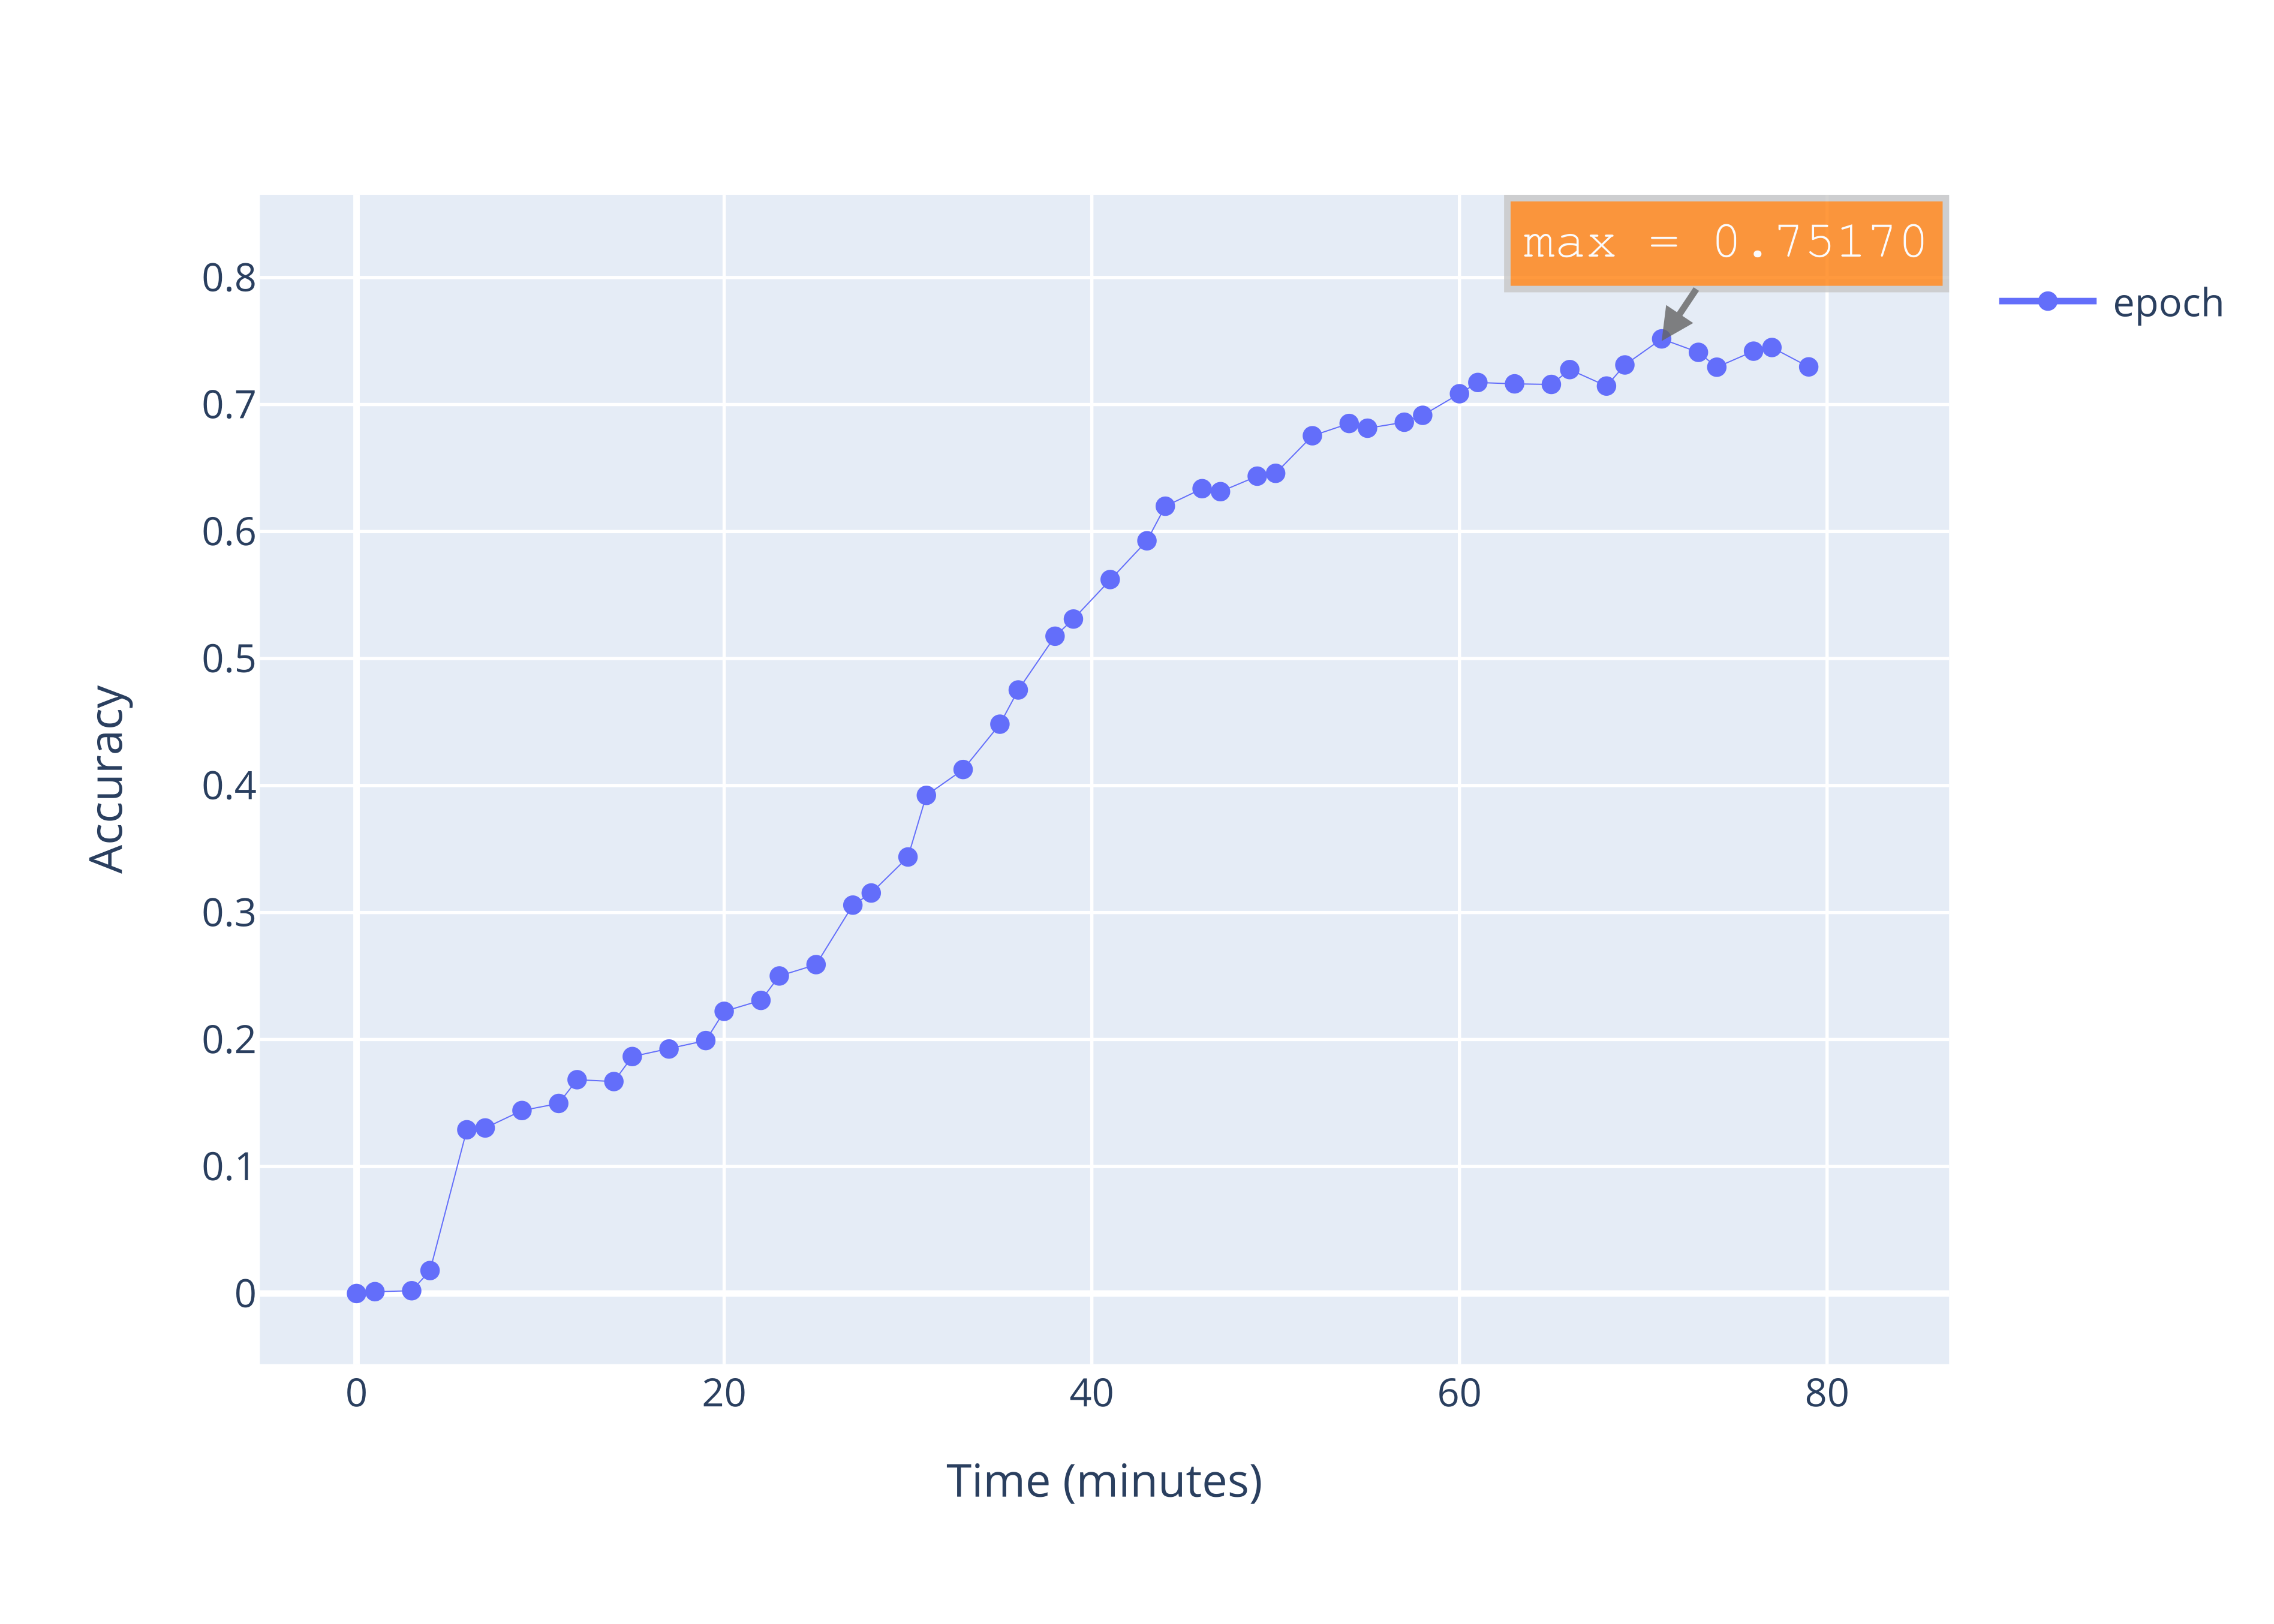
\includegraphics[width=1.1\textwidth]{annexes/graph/train_epoch.png}
	    \caption{Entraînement d'un modèle avec la méthode \textit{skratch}}
	    \label{fig:epoch_skratch}
	\end{figure}
	
	Le moteur développé par Benjamin Kiessling permet de créer son modèle à partir de deux méthodes de \textit{machine learning} : le modèle \textit{skratch} dont les données d'apprentissages sont natives ce qui signifie un apprentissage \textit{ad hoc}, et la technique du \textit{transfert learning} qui correspond à la réutilisation d'un modèle pré-entrainé et d'en exploiter les connaissances basiques en reprenant son architecture et en y ajoutant des données \textit{ad hoc}. L'entraînement \textit{via fine-tuning} est donc une sous catégorie du \textit{transfert learning}, assez propre aux architectures \gls{CNN}, puisque cette méthode permet de réadapter les poids neuronaux au cours de l'apprentissage ce qui conduit à affiner le modèle. Il faut penser qu'au sein du réseau neuronal, les neurones situés en premières séries ont très souvent des tâches génériques alors que les dernières séries de neurones ont la plus grande part une fonction très spécifique. Tout l'enjeu de ce procédé est finalement d'affiner les poids de ces derniers.
	
	Les avantages du \textit{transfert learning} puisqu'il est désormais possible de produire des modèles performants à moindre coût, en limitant le besoin de produire des données terrains\footcite{aradillasBoostingHandwritingText2018}. Coupler les données en puisant sur des neurones existants permet généralement d'obtenir de très bon, voir d'excellents résultat. Vincent Jolivet estime aujourd'hui que le fine-tuning est devenu la norme au sein du paysage de la \gls{rem}, en permettant de créer des modèles à moindre coût \footcite{torresHTRFineTuning2022}. La multiplication des plateformes de partage de données et de modèles est ainsi indispensable au développement de cette stratégie, et \textit{de facto} à la démocratisation de l'\gls{htr}.
	
	\subsection{Modélisation, résultats et interprétations}
	
	Afin d'observer concrètement les avantages et les inconvénients de ces deux méthodes, plusieurs modèles ont été réalisés afin de déterminer le réseau neuronal le plus performant pour déchiffrer des sources manuscrites de multiples mains\footnote{Les lignes de commandes utilisées avec le moteur kraken sont observables en annexe (voir figure \ref{code:skratch} et \ref{code:finetuning}}).
	
	\subsubsection{\textit{Datasets} et modèles}
	
	En plus des données produites, deux jeux de données extérieurs ont été utilisés : les archives notariales du projet \gls{lectaurep} et le modèle éponyme, ainsi que les archives des testaments de poilus\footcite{durandNotairesParisRepertoires2021, clericeCREMMAANTestamentDePoilus2022}. Ces deux \textit{datasets} peuvent être rapprochés de nos données terrains, car ils sont composés de documents avec une écriture cursive contemporaine (XIX\textsuperscript{e} siècle). 
	
	La difficulté consiste à disposer de suffisamment de données terrains propres afin de \enquote{casser le modèle de langue}, car on le rappelle, les moteurs \gls{htr} s'appuient sur le traitement du langage pour affiner ces prédictions. Enfin, nous nous sommes fondés sur le récent méga-modèle \textit{Manu MacFrench} développé par Thibault Clérice et Alix Chagué\footcite{chagueHTRUnitedManuMcFrench2022}.
	
	
	\subsubsection{Résultats et analyses}
	
	\begin{table}
    \centering
    \resizebox{\textwidth}{!}{%
    \begin{tabular}{|l|l|l|l|l|l|}
    \hline
    \multicolumn{1}{|c|}{\textbf{Name}} & \multicolumn{1}{c|}{\textbf{Quantity (GT)}} & \multicolumn{1}{c|}{\textbf{Val\_acc}} & \multicolumn{1}{c|}{\textbf{Test\_acc}} & \multicolumn{1}{c|}{\textbf{CER}} & \multicolumn{1}{c|}{\textbf{WER}} \\ \hline
    ArSKR                               & 180                                         & 0.75170                                & 0.77860                                      & 0.26558                                & 0.38640                                \\ \hline
    ArLCTP                              & 144                                         & 0.93328                                & 0.83570                                      & 0.04410                                & 0.18993                                \\ \hline
    ArLCTP-NFKD                         & 144                                         & 0.91871                                & 0.84650                                      & 0.03668                                & 0.15853                                \\ \hline
    ArLCTP+pl                           & 244                                         & 0.91697                                & 0.83230                                      & 0.05045                                & 0.21338                                \\ \hline
    ArMcFR                              & 180                                         & 0.90354                                & 0.86730                                 & 0.05598                                & 0.21423                                \\ \hline
    ArMcFR-NFKD                         & 180                                         & 0.89872                                & 0.85630                                      & 0.06646                                & 0.24963                                \\ \hline
    \end{tabular}%
    }
    \caption{Résultats des modèles HTR\protect\footnotemark}
    \label{tab:results_htr}
    \end{table}
    
    \footnotetext{ArSKR : modèle \textit{skratch dataset ad hoc}; ArLCTP : \textit{fine-tuning} avec modèle \gls{lectaurep}; ArLCTP+pl : \textit{fine-tuning} avec modèle \gls{lectaurep} et ajout du jeu de données des testaments de poilus; ArMcFR : \textit{fine-tuning} avec modèle \textit{Manu MacFrench}.}
    
    Comme nous pouvons le constater au sein du tableau \ref{tab:results_htr}, les différentes méthodes employées ont affichés des résultats assez contrastés. La valeur \gls{ACC} proposée par kraken lors du processus d'entraînement a rapidement été insuffisante pour comparer et optimiser le caractère. Lors de la compilation préalable des fichiers, la désignation des fichiers tests est donc hasardeuse et les résultats obtenus sont alors intrinsèquement relatifs. Dans un premier temps, nous nous sommes appuyés sur l'application \texttt{KaMi-Lib} développée par l'\gls{inria} et plus particulièrement Lucas Terriel\footcite{terrielKaMIlib2022}. Elle permet d'étendre le nombre de mesures possibles afin d'étudier plus en profondeur les prédictions \gls{ocr} en fonction des vérités terrains, mais aussi d'obtenir certains mesures relevant du \gls{tal}. Au sein de chaque main principale, un échantillon a été prélevé afin de constituer les données de terrains de l'évaluation par \texttt{KaMi-Lib}\footcite{humeauHTREvaluation2022}. Les principales mesures qui ont été utilisées pour comprendre l'efficacité des modèles \gls{rem} sont les métriques \gls{CER} et \gls{WER}, permettant de donner le taux d'erreurs par caractères et par mots. En parallèle, un jeu de données tests a été constitué afin de déterminer le taux \gls{ACC} à partir d'une main inconnue et de qualité moyenne. 
    
    À première vue, le modèle ArLCTP, \textit{fine-tuned} à partir du modèle déployé par le projet \gls{lectaurep}, semble donner les meilleurs résultats. En revanche, en le comparant aux données issues de l'évaluation test, le taux \gls{ACC} est bien plus faible, laissant penser à un possible phénomène d'\textit{overfitting} en raison de sa mauvaise adaptation. Le modèle ArMcFR semble ainsi offrir les résultats les plus polyvalents et indiquant une meilleure performance malgré des taux \gls{CER} et \gls{WER} légèrement plus élevés. Il reste tout de même perfectible en vue de ces résultats pouvant être qualifiés de \enquote{moyen-bon} en raison de ses taux d'erreurs\footcite[Dans cette article, il est estimé que le \gls{CER} doit être inférieur à 2 afin d'être qualifié de très bon voir d'excellent]{tomoiagaFieldTypingImproved2019}. Lors du colloque \enquote{Documents anciens et reconnaissance automatique des écritures manuscrites} qui se déroulait en juin 2022, Vincent Jolivet et Sergio Torres ont estimé qu'un taux \gls{ACC} de 90\% doit être comme considéré comme le seuil sur l'échelle du rapport coût de production et efficacité du modèle\footcite{torresHTRFineTuning2022}. De même, Maciej Eder estime que le bruit des données au sein des corpus textuels n'affecte pas singulièrement les recherches autour, la stylométrie dans ce cas précis, si le taux de corruption des données est inférieur à 20\%\footcite{ederMindYourCorpus2013}.
    
    Toutefois, il reste à évaluer la capacité du modèle à être affiné selon les situations. Sans avoir pu être réalisée en l'état, l'agrégation de quelques nouvelles données terrains sur une main bien particulière pourrait permettre d'atteindre des taux extrêmement satisfaisants comme le souligna Ariane Pinche au cours de ce même colloque\footcite{pincheSegmOntoControlledVocabulary2022a}.
	
	\subsubsection{Difficultés et encodage}
	
	En reprenant le tableau \ref{tab:results_htr}, on peut constater la présence de modèles NFKD (\textit{Normalization Form Canonical Decomposition}). Il s'agit d'un système d'uniformisation au sein des caractères Unicode. La méthode NFKD permet dans ce cas de décomposer les caractères diacritiques, en un ensemble de caractères Unicode permettant une appréhension fondamentale, en conservant sa relation canonique et ordonnée. Les divers essais montrent une appropriation relative des modèles \gls{htr} à cette uniformisation. On remarque au sein du tableau \ref{tab:error_htr} que la gestion des accents représente le sixième type d'erreurs les plus fréquentes.
	
	\begin{table}
    \centering
    \resizebox{0.4\textwidth}{!}{%
    \begin{tabular}{|c|c|c|}
    \hline
    \textbf{Nombre} & \textbf{Correct} & \textbf{Généré} \\ \hline
    40              & s                & c               \\ \hline
    24              & SPACE            & NONE            \\ \hline
    22              & i                & e               \\ \hline
    21              & o                & a               \\ \hline
    21              & r                & s               \\ \hline
    20              & ACCENT           & NONE            \\ \hline
    18              & s                & r               \\ \hline
    \end{tabular}%
    }
    \caption{Les 7 erreurs les plus courantes du modèle ArMcFR}
    \label{tab:error_htr}
    \end{table}
    
    En examinant plus attentivement les erreurs récurrentes du modèle, on peut rapidement identifier plusieurs lacunes et confusions, en particulier la reconnaissance des caractères Unicode 'r' et 's'. Cette répétitivité amène à un \gls{WER} moyen indiquant un mot erroné tous les cinq mots. Ces confusions peuvent s'expliquer par la fréquence élevée de ces caractères au sein de la langue espagnole et de la proximité graphologique entre les caractères. 
    
    \begin{figure}
        \centering
        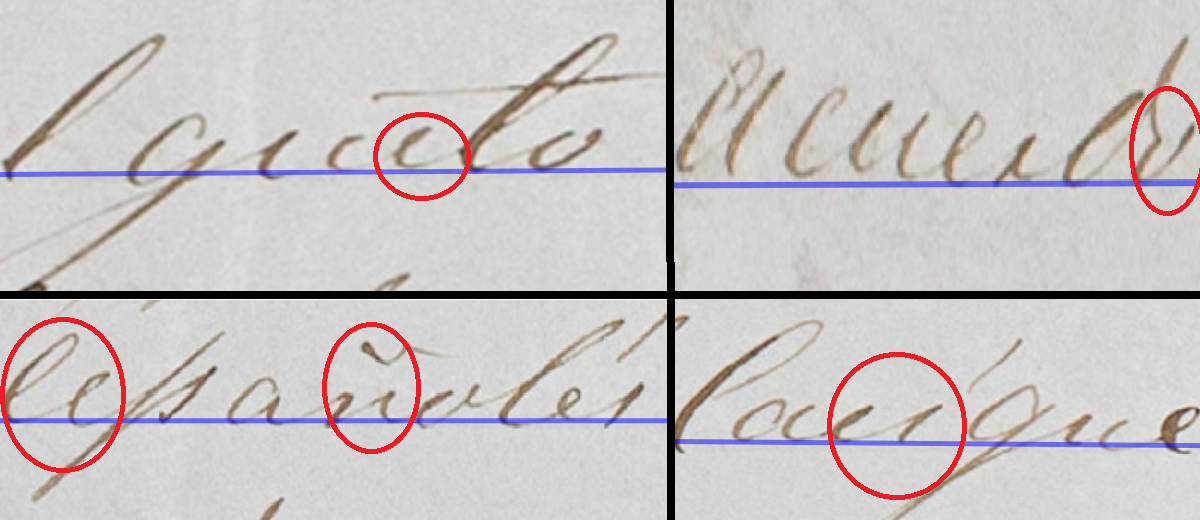
\includegraphics[width=0.9\textwidth]{annexes/img/error_HTR.png}
        \caption{Exemple d'erreurs courantes pour le modèle ArMcFR\protect\footnotemark}
        \label{fig:error_htr}
    \end{figure}
    
    \footnotetext{Image haut gauche : guito/ gusto; image haut droite: acuerd/acuerdo; image bas gauche: lepanoles/españoles; image bas droite: Caesque/Cacique.}

    
    En observant plus en détail, la distance des mots, selon l'algorithme de distance de Levenshtein, se situe autour d'une moyenne tronquée autour de 43, mais avec un écart-type plus conséquent concernant les mains Villalon et Saavedra. Cette distance semble \textit{a priori} suffisamment faible indiquant une relative concordance entre les mots prédits et les mots corrects, limitant le risque d'altérer le sens initial\footcite{terrielAtelierProductionModele2021}. À partir de cette distance, Thi-Tuyet-Hai Nguyen et al. classe deux types d'erreurs : les erreurs simples et les erreurs complexes ayant un nombre d'erreurs supérieur à 1\footcite{nguyenDeepStatisticalAnalysis2019}. Ces erreurs vont plus ou moins être influencées selon la longueur des mots et la gestion des espacements des modèles \gls{ocr} et ainsi augmenter le risque de cette distance.
    
    Il est donc toujours difficile d'évaluer correctement un modèle, et plus encore, de sélectionner le modèle le plus performant dans le cadre d'une application contrainte et spécifique. Dans notre cas, nous sommes appuyés sur des métriques basées sur le lexique dont le modèle ArMcFR semble ressortir comme le plus complet. Cependant, à l'heure de la massification des solutions \gls{tal} certaines mesures pourraient reprendre les évaluations par système de masque sur le modèle des architectures encodeurs-décodeurs comme le constatent Phillip Benjamin Strobel et al.\footcite{strobelEvaluationHTRModels2022}.
    
    \begin{figure}[H]
	    \centering
	    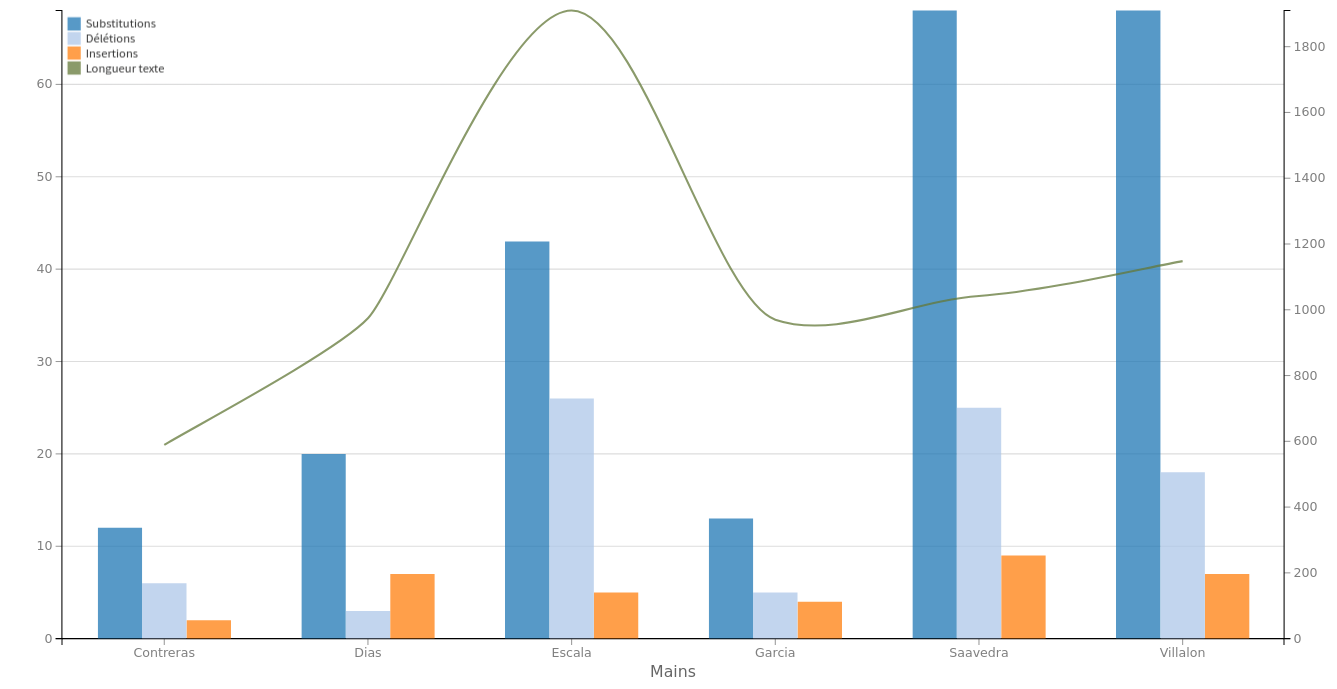
\includegraphics[width=0.9\textwidth]{annexes/graph/DIS_htr.png}
	    \caption{Évaluation \gls{DIS} du modèle ArMcFR avec \texttt{KaMi-Lib}}
	    \label{fig:dis_htr}
	\end{figure}
	
	
	\subsection{Les difficultés d'un modèle de segmentation}
	
	À partir de notre lot de transcriptions, nous avons dans le même temps essayer de produire un modèle de segmentation \gls{htr} à partir du moteur \gls{kraken}. Il fait suite à la volonté d'automatiser la segmentation des zones et des lignes à partir de l'ontologie prédéfinie ultérieurement.
	
	Pour se faire, nous avons repris le modèle de segmentation par défaut développé par l'équipe de Scripta afin de procéder à un entraînement par \textit{finetuning}. Le développement du modèle \texttt{blla} s'est appuyé sur le jeu de donnée qui a remporté la compétition ICDAR de 2017. Il propose un modèle minimaliste possédant de hauts taux de performance sur la détection de ligne et de zones (bounding boxes) et permettre à des modèles sémantiques de s'appuyer sur cette base\footcite{kiesslingBADAMPublicDataset2019}.
	
	\begin{figure}
	    \centering
	    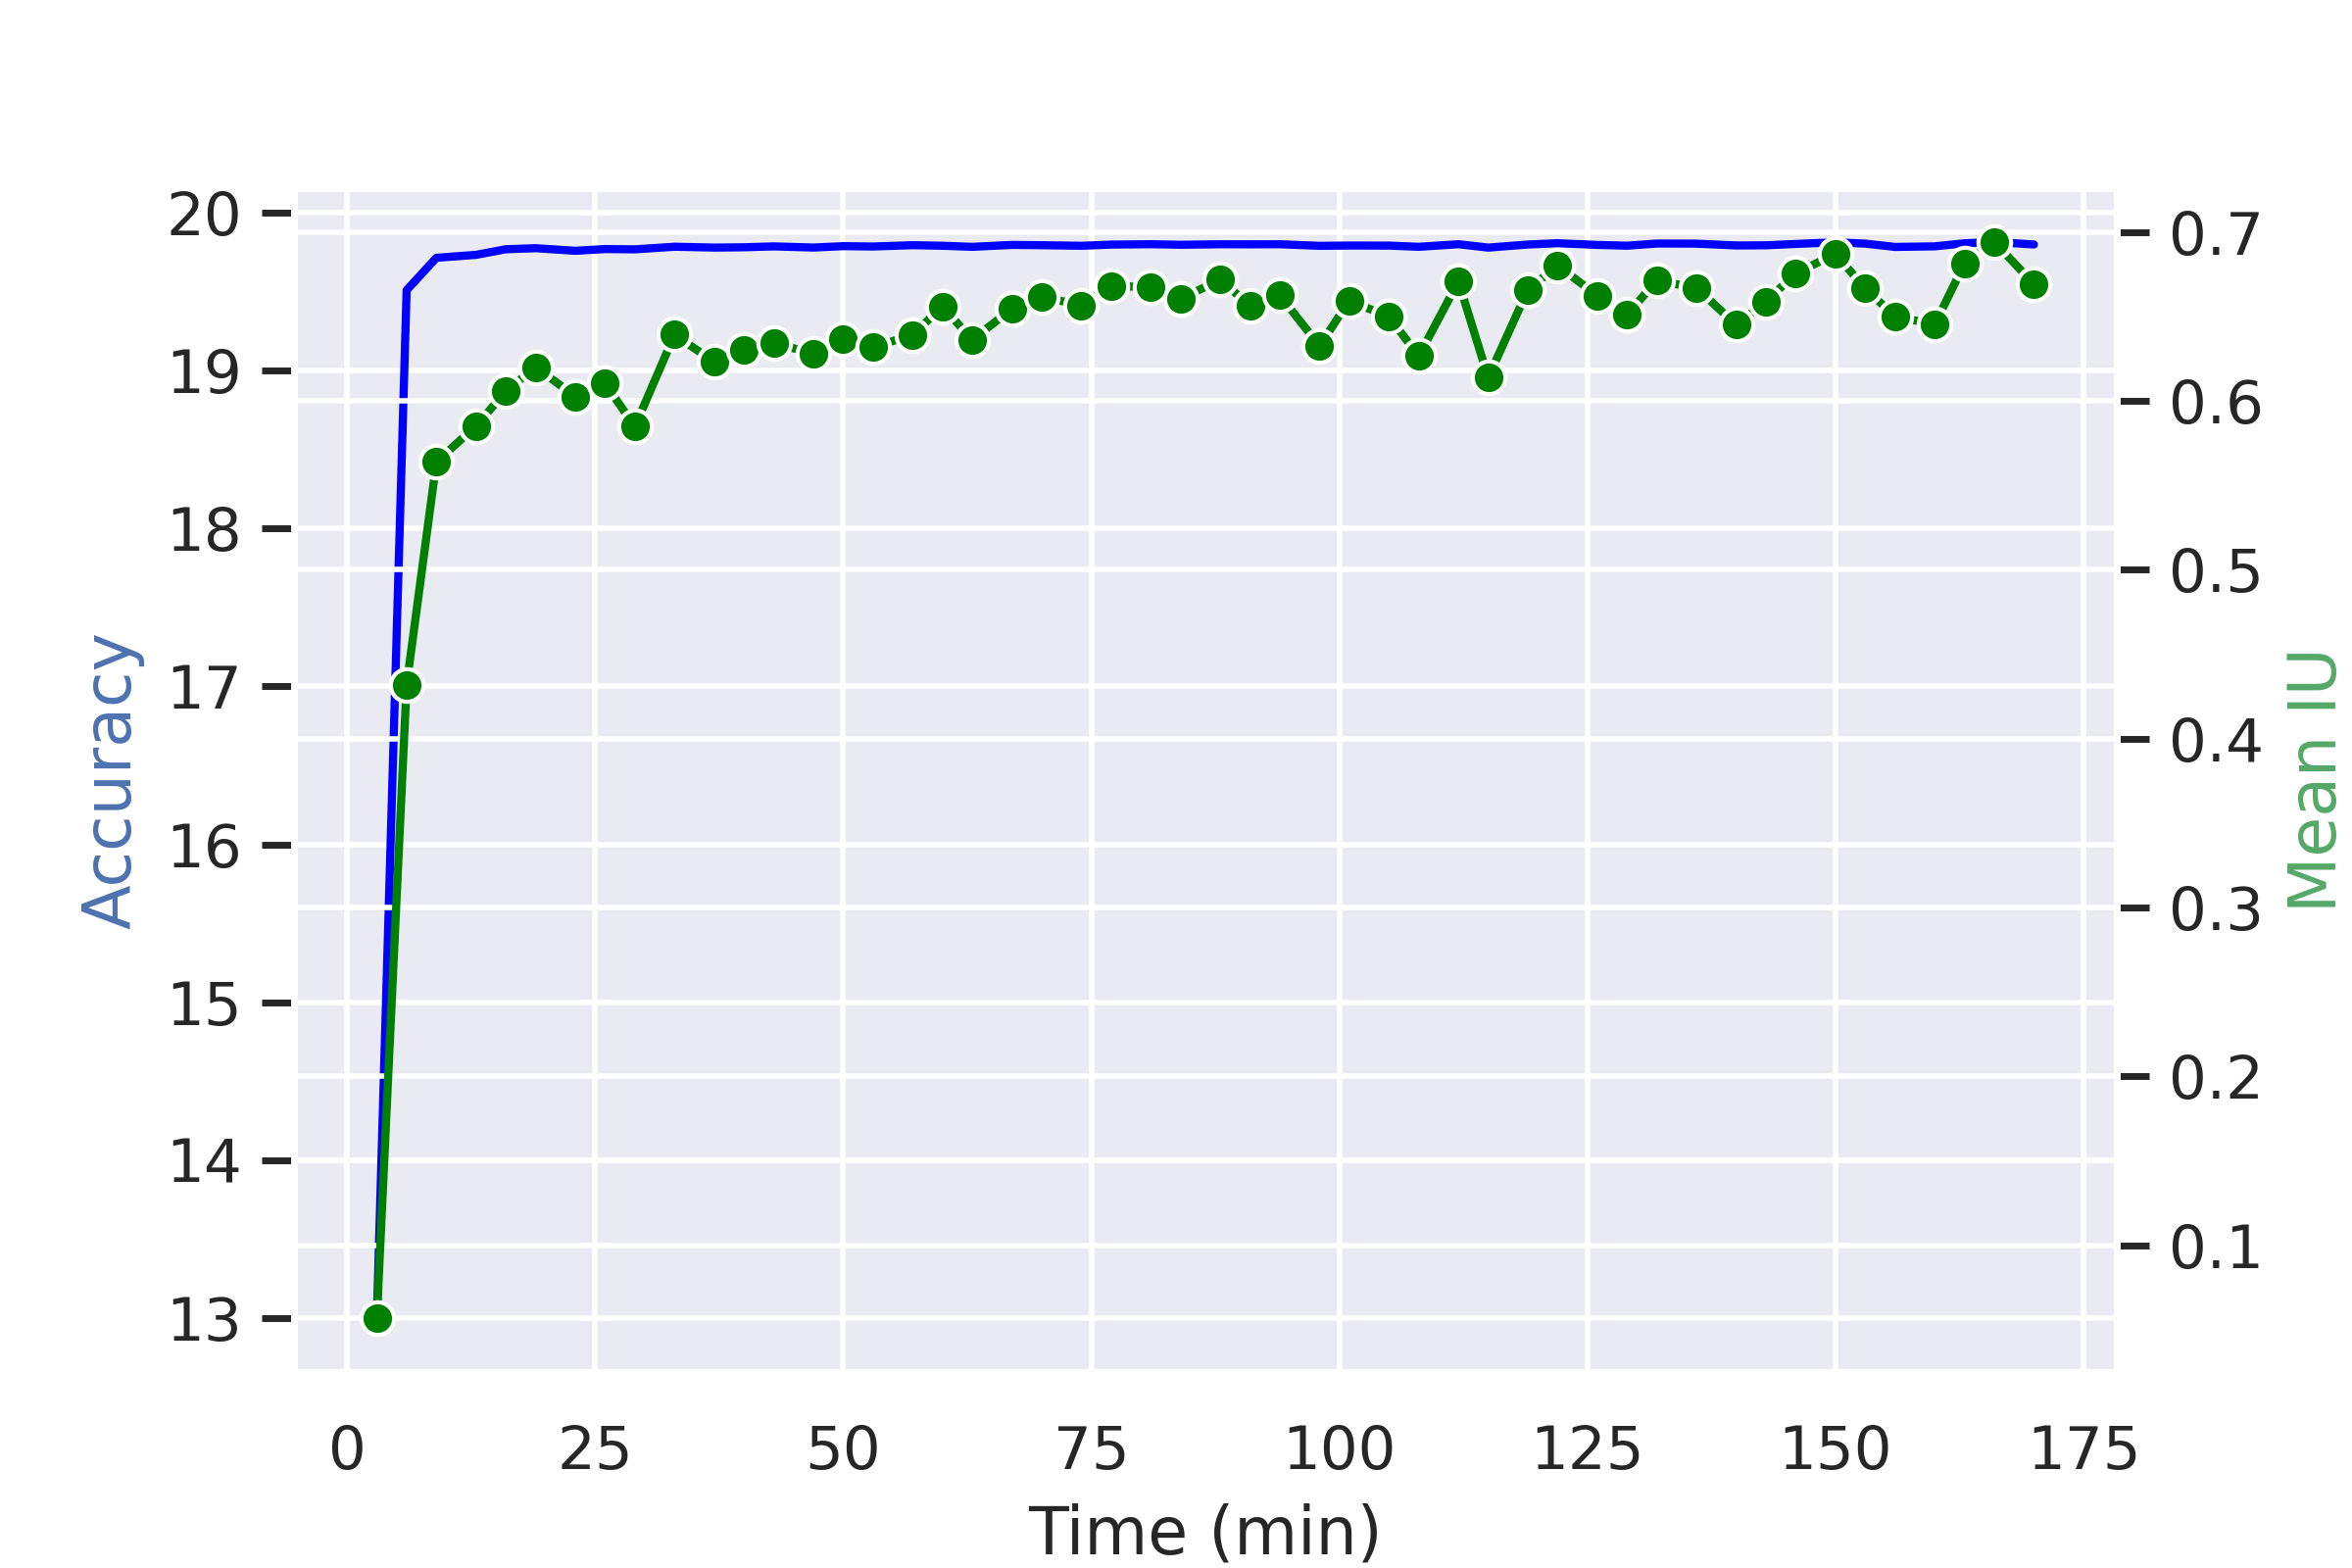
\includegraphics[width=0.6\textwidth]{annexes/graph/epoch_segtrain.png}
	    \caption{Le processus d'entraînement du modèle ArSeg}
	    \label{fig:epoch_mode}
	\end{figure}
	
	\begin{table}[]
	    \centering
        \begin{tabular}{|l|l|l|l|l|}
        \hline
        \multicolumn{1}{|c|}{\textbf{Model}} & \textbf{val\_acc} & \textbf{mean\_acc} & \textbf{mean\_iu} & \textbf{freq\_iu} \\ \hline
        \textbf{ArSeg}                       & 19.81395          & 19.81395           & 0.69404           & 0.69404           \\ \hline
        \end{tabular}
        \caption{Evaluation des performances du modèle ArSeg}
        \label{tab:ArSeg_benchmark}
    \end{table}
	
	L'entraînement sur nos documents historiques a été exécuter sur la base des recommandations établis par Juliette Janès et al. pour l'entraînement d'un modèle de mise en page\footcite{janesAutomaticTEIEncoding2021a}. La commande shell (retrouvable au sein de l'annexe D, voir \ref{code:segment}) reprend ainsi le réseau neuronal défini préalablement.
	
	Néanmoins, les résultats affichés durant l'entraînement démontrent de nombreuses fragilités. L'évaluation d'un modèle de segmentation s'est axé sur deux systèmes mesures : le \textit{mean Intersection-Over-Union} (Mean IU) qui reprend l'ensemble de l'indice de Jacard calculant la similarité entre deux éléments et le taux d'alignement;  le mean Accuracy calcule la moyenne de toutes les classes sur le principe de la métrique \gls{ACC}\footnote{Pour plus de détails, les explications faites par Hugo Scheithauer sont très explicites. \cite[p.~79-80]{scheithauerReconnaissanceEntitesNommees2021}}. 
	
	Comme le démontre la figure \ref{fig:segment_model}, les prédictions affichent un manque de régularité sur l'appréciation des \textit{baselines} et des zones. Les lignes en marge du document sont quant à elles ignorées ou très mal déterminées. De même, on observe que seules les zones \textit{Main:text} et \textit{QuireMarksZone:signature} sont identifiées. Ce dernier point peut démontrer le besoin de simplifier l'ontologie.
	
	\begin{figure}[p]
	    \centering
	    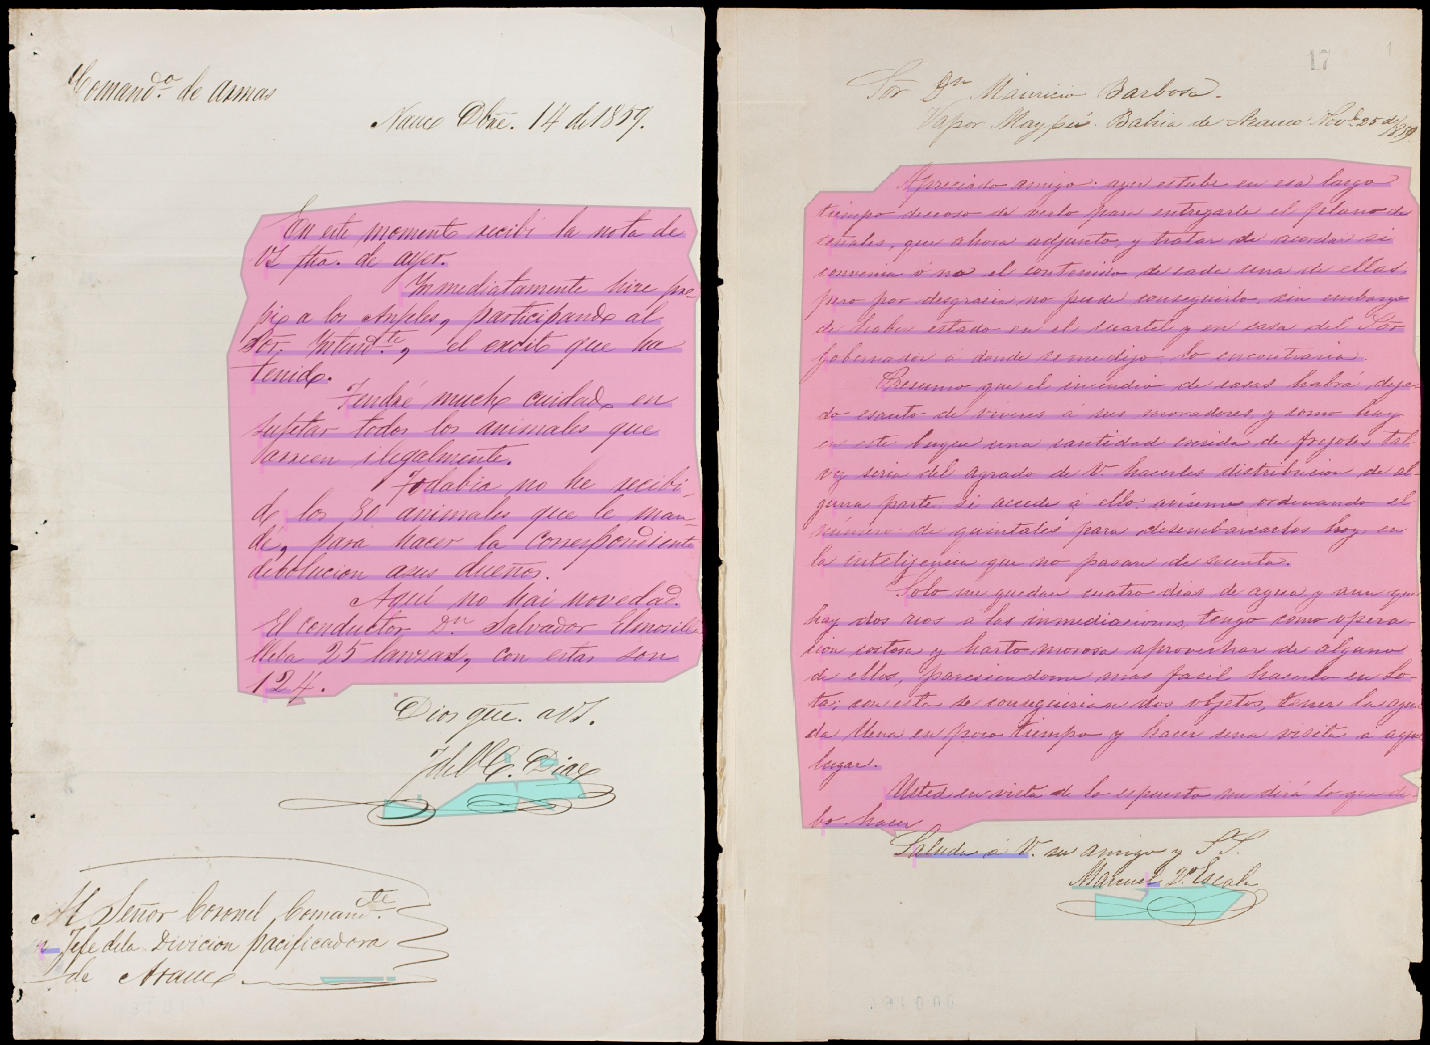
\includegraphics[width=1\textwidth]{annexes/img/segment_model.png}
	    \caption{Exemple de segmentation à partir du modèle ArSeg}
	    \label{fig:segment_model}
	\end{figure}
	
    Face à ce constat, le modèle ne permet pas d'obtenir une segmentation efficiente  et exploitable afin de l'intégrer au sein du flux éditorial. Une segmentation manuelle à partir du modèle par défaut proposé sur la plateforme \gls{eScriptorium} reste privilégiée au cours de cette chaîne de traitement afin de réévaluer les données d'entraînements.
    
	Les récents résultats présentés par Thibault Clérice peuvent laisser un espoir d'amélioration du système de segmentation\footcite{clericeYouActuallyLook2022}. Il propose de déplacer, par souci d'efficacité, la reconnaissance non plus sur une polygonisation basée sur la classification des pixels, mais à une détection d'objet utilisant des rectangles isothétiques. Pour cela, il appuie l'incorporation du moteur \texttt{YOLOv5} au sein du moteur \gls{kraken}.
	
	\section{La gestion des erreurs : le post-traitement comme second souffle à l'HTR}
	\sectionmark{Le post-traitement HTR}
	
	La reconnaissance automatique de texte ne s'arrête pas aux seuls prédictions du modèle \gls{htr}. Depuis les années 1990, de nombreux projets se sont appuyés sur le post-traitement des prédictions afin d'améliorer la qualité, en s'appuyant notamment sur des modèles statistiques aux frontières de la linguistique, en particulier les systèmes d'occurrences séquentielles (n-grammes) \footcite{takahashiSpellingCorrectionMethod1990, tongStatisticalApproachAutomatic1996}.
	
	Nous allons observer comment le projet Araucania a tenté de prolonger cette chaîne de traitement \gls{htr} en procédant à une mise en place d'une post-correction automatique. Le but est de réduire significativement les erreurs issues des transcriptions grâce à l'aide d'un corpus témoin.
	
	\subsection{Principe de la Distance de Levenshtein}
	
	Les erreurs des prédictions \gls{ocr} et \gls{htr} se résument à des erreurs de substitutions, d'insertions ou de suppressions de caractères au sein d'un ou plusieurs mots. Ces altérations au sein d'un mot transcrit peuvent être décrit à travers la distance de Levenshtein. Cette mesure de la différence entre deux chaînes de caractères a été proposée sous la forme d'un algorithme linguistique par le mathématicien russe Vladimir Levenshtein en 1965. Le principe y est assez simple, plus la distance est élevé, plus le mot transcrit a donc subi d'altérations. 
	
	\begin{wrapfigure}[7]{r}{9cm}
        \centering
        
\includegraphics[width=7.5cm]{annexes/img/leventshein.png}
        \caption{Algorithme de Levenshtein - @wikipedia}
        \label{fig:algo_levenshtein}
    \end{wrapfigure}
    
    Dès la fin des années 1990, certains ingénieurs se sont essayer à intégrer cette distance dans leur chaîne de traitement \gls{ocr} afin d'estimer les candidats correctifs les plus prometteurs à partir de calculs probabilistes selon des séquences de caractères et de mots (n-grammes) texte\footcite{tongStatisticalApproachAutomatic1996}. Depuis, d'autres projets ont essayer d'intégrer cette mesure grâce à l'appui de dictionnaires d'occurrences, classification de mots, séquence de caractères notamment pour les problèmes de segmentations entre les mots\footcite{kissosOCRErrorCorrection2016, haldarLevenshteinDistanceTechnique}. Les différentes méthodes ont permis de réduire le nombre d'erreurs des prédictions \gls{ocr} jusqu'à 30\%. En ce sens, nous remarquons l'initiative du projet \gls{dahn} dirigé par Floriane Chiffoleau qui introduit une correction \textit{via} la distance de Levenshtein\footcite{chiffoleauDAHNProjectDigital2022}.
	
	\subsection{Mise en place d'une correction automatisée}
	
	Sur le modèle du projet \gls{dahn}, nous avons expérimenté la mise en place d'un CLI correctif au sein de la chaîne de traitement. Le script s'est fondé plus exactement sur l'incorporation de la librairie python \texttt{PySpellchecker}, et secondairement la librairie de \gls{tal} \gls{spacy} \footcite{barrusPyspellchecker2022}.
	
	\texttt{PySpellchecker} intègre un système de correction statistique à partir d'un dictionnaire d'occurrence, en appliquant la distance de Damerau-Levenshtein pour identifier les altérations possibles et une détermination des candidats grâce au théorème de Bayes, permettant de déterminer la probabilité d'un évènement par rapport à d'autres\footcite{norvigHowWriteSpelling2007}. L'idée est donc de générer l'ensemble des possibilités dans la limite de cette distance, et choisir le candidat le plus plausible. En ce sens, le dictionnaire d'occurrences permet de sélectionner le candidat à partir de ces calculs probabilistes, l'inférence bayésienne c'est-à-dire la démarche logique permettant de calculer ou actualiser la probabilité d'une hypothèse.\footcite[Récemment cette technique est encore recommandée, avec une amélioration de près de 30\% des cas comme le révèle cette étude.][]{haldarLevenshteinDistanceTechnique}.
	
	\begin{equation}
    \label{eq:bayes}
    P(\alpha|\beta) = \frac{P(\beta |\alpha)P(\alpha)}{P(\beta)}
    \end{equation}
    
    La complexité de la correction est décrite par un article publié en 2019 qui étudie statistiquement les erreurs récurrentes au sein des mécanismes \gls{ocr}\footcite{nguyenDeepStatisticalAnalysis2019}. Comme évoqué en amont, le groupe de chercheurs décrivent deux types d'erreurs fondamentales. La détection de ces erreurs multiples est corrélée à une distance plus grande, multipliant par conséquent le nombre de candidats possibles et donc accroissement du bruit. Au vu des résultats du modèle ArMcFR, nous avons estimé qu'une distance de 2 serait suffisante au vue d'une distance moyenne par mot assez faible (43) sur l'ensemble de la transcription, indiquant une répartition plus forte des erreurs (WER de 21\%). \newpar
    
    Comme l'indique le schéma du script suivant (voir figure \ref{fig:postprocess}), le processus s'est basé sur les recommandations de Daniel Lopresti dans la construction d'une chaîne de traitement post-OCR\footcite{loprestiOpticalCharacterRecognition2009}. Ligne par ligne, les phrases subissent un processus de tokénisation afin d'en révéler les informations essentielles, et de pouvoir traiter les mots individuellement. Le dictionnaire d'occurrences comme corpus de contrôle a ainsi été construit autour des données terrains produites précédemment afin d'aligner le niveau de langue de nos documents historiques avec nos prédictions \gls{htr}\footcite{humeauPostprocessHTR2022}. Les dictionnaires par défaut sont davantage adaptés aux corrections des productions très contemporaines.
	
	\begin{figure}[h!]
	    \centering
	    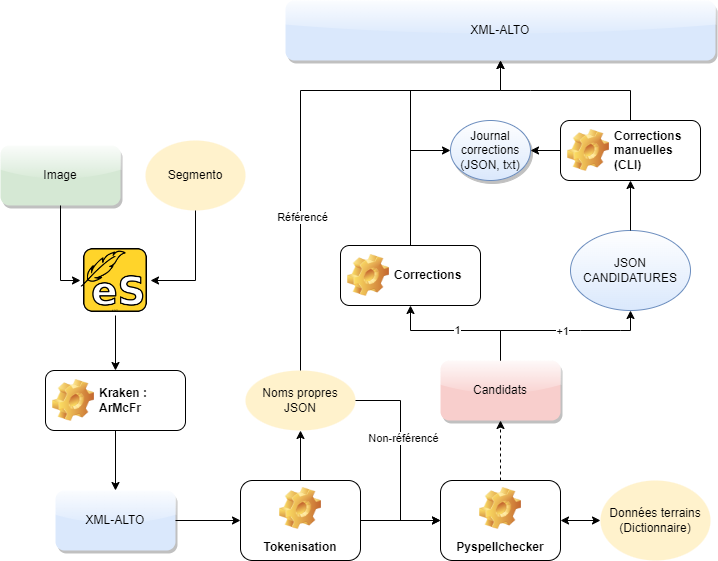
\includegraphics[width=0.8\textwidth]{annexes/schema/post_traitement.png}
	    \caption{Schéma de traitement des prédictions HTR}
	    \label{fig:postprocess}
	\end{figure}
	
	Une des premières étapes est de sélectionner les tokens dont la nature (POS, \textit{part of speech} en anglais) est un nom propre afin d'être identifiée au sein d'un répertoire de noms propres géographiques\footnote{Le dictionnaire JSON s'appuie sur un dictionnaire du XIX\textsuperscript{e} siècle : \cite{solanoasta-buruagaDiccionarioGeograficoRepublica1899}. Le dictionnaire a été produit \textit{via webscrapping} dont le script est disponible ici : \cite{humeauEnrichmentWikisource2022}}. S'il n'est pas détecté il est donc retourné comme erreur au sein du processus de correction. Ce procédé permet de pallier au limite du dictionnaire d'occurrences construit sur des données préalablement identifiées. Certains lieux lui sont donc encore inconnus, relevant ainsi d'une erreur.
    
    Selon les erreurs détectées et retournées, les candidats sont alors soumis à un processus de sélection restrictif, et ce en fonction d'une distance limite de 2 entre le mot identifié et les propositions faites. Si les propositions sont au nombre de 1 alors, le fichier \gls{alto} est automatiquement édité avec la correction sélectionnée. En revanche, si la liste des propositions est égale à zéro ou supérieure à 1 alors les données sont enregistrées au sein d'un fichier \gls{json} afin d'être corrigées manuellement.
	
	\subsection{Résultats et améliorations}
	
	Afin d'évaluer la performance du traitement correctif des fichiers \gls{htr}, nous avons réalisé une analyse textuelle comparative grâce à la librairie \texttt{KaMi-Lib} à partir d'un échantillon de quatre fichiers de notre jeu de données test. Les prédictions basiques ont été effectuées avec le modèle ArMcFr, puis comparées aux mêmes données transformées par le script de corrections. Malgré quelques tentatives d'améliorations, les résultats se sont montrés assez décevants pour le moment comme le montre le tableau de comparaison \ref{tab:erreurs_compa}. 
	
	Étonnamment, les premières mesures indiquent une augmentation des métriques \gls{CER} et \gls{WER} pouvant signaler une forte distorsion provoquée par la correction automatique. En revanche, les évaluations complémentaires indiquent une très légère progression concernant la distance entre la prédiction \gls{htr} et la correction proposée et les altérations de caractères. L'augmentation des mesures \gls{CER} et \gls{WER} pourraient donc s'expliquer par une réduction des caractères totaux et une plus forte disparité entre les mots corrigés positifs et les mots corrigés négatifs notamment à cause d'une mauvaise gestion des accents.
	
	\begin{table}[h]
	\centering
    \begin{tabular}{l|cc|c|}
    \cline{2-4}
                                        & \multicolumn{1}{l|}{\textbf{Prediction}} & \multicolumn{1}{l|}{\textbf{Correction}} & \multicolumn{1}{l|}{\textbf{Différence}} \\ \hline
    \multicolumn{1}{|l|}{CER (\%)}           & 13.58                                    & 13.77                                    & +0.19                                    \\ \cline{1-1} \hline
    \multicolumn{1}{|l|}{WER (\%)}           & 45.48                                    & 42.56                                    & +2.92                                    \\ \cline{1-1} \hline
    \multicolumn{1}{|l|}{D\textsubscript{mots}}   & 77                                       & 72                                       & -5                                       \\ \cline{1-1} \hline
    \multicolumn{1}{|l|}{Insertions}    & 13.25                                    & 11.25                                    & -2                                       \\ \cline{1-1} \hline
    \multicolumn{1}{|l|}{Deletions}     & 19.25                                    & 17                                       & -2.25                                    \\ \cline{1-1} \hline
    \multicolumn{1}{|l|}{Substitutions} & 91                                       & 87.75                                    & -3.25                                    \\ \cline{1-1} \hline
    \end{tabular}
    \caption{Analyse des effets du traitement automatique des erreurs HTR}
    \label{tab:erreurs_compa}
    \end{table}
    
    Nous pouvons émettre plusieurs constats d'améliorations à la suite de notre analyse de cas. La première difficulté réside dans la gestion des noms propres, et ce malgré le filtrage à partir du POS, dont la détermination se révèle souvent erronée. Dans de nombreux cas, les noms géographiques ont été abrégés au sein des transcriptions, complexifiant grandement l'opération de correction. L'autre point est la gestion dans sa globalité des noms propres comme le renseigne Hugo Scheithauer, après quelques expérimentations pour le projet \gls{lectaurep}\footcite[p.~88-89]{scheithauerReconnaissanceEntitesNommees2021}.
	
	La seconde difficulté, et sans doute la plus grande, réside dans la détection des erreurs au sein des mots réels (40\%)\footcite{nguyenDeepStatisticalAnalysis2019}. À l’inverse d'un mot non-réel, le mot réel signifie que les altérations DIS ont transformés le mot initial en un autre mot existant et référencé. Nous l'avons vu, l'orthographe est très variable et ponctuée de fautes au sein des archives. Ces différences linguistiques amènent donc une difficulté à identifier les erreurs \gls{htr} avec les variations orthographiques et les erreurs orthographiques originales. De plus, ces variations, volontaires ou non, augmentent artificiellement le nombre de mots existants, biaisant le dictionnaire d'occurrences et donc les probabilités bayésiennes. Une solution pourrait s'imaginer avec l'introduction d'un processus de lemmatisation entre le produit \gls{htr} et le corpus contrôle, et une meilleure utilisation de l'étiquetage de la parole (POS). \newpar
	
	Comme signalé par Youness Chaabi et Fadoua Ataa Allah, le système Norving employé par la librairie \texttt{PySpellchecker} possède de nombreuses limites\footcite{chaabiAmazighSpellChecker2022}. Le système de classification par dictionnaire d'occurrences est éprouvé depuis très longtemps qui bien que conçu pour être effectué au travers de calcul simple, celui-ci est connu pour générer un trop gros nombre de résultats\footnote{Même si le nombre est alors limité par la définition de la distance de Levenshtein.}. De plus, l'effet de contextualisation du mot erroné au sein de la phrase est assez limité. En ce sens, une combinaison entre le système Norvik et l'utilisation de l'analyse séquentielle par N-grammes pourrait permettre l'obtention de meilleurs résultats comme le proposent les chercheurs de l'Université du Roi-Saoud\footcite{chaabiAmazighSpellChecker2022}.
	
    Lors du concours de l'IDCAR 2019, l'utilisation de cette architecture est remarquée puisque le modèle BERT démontre un fort potentiel dans la résolution de correction contextuelle\footcite{rigaudICDAR2019Competition2019}. Par la suite, plusieurs groupes de chercheurs ont mis à profit ces résultats primaires afin de construire de nouvelles expérimentations avec les architectures \gls{tal} encodeurs-décodeurs (BERT, RoBERTa, etc.)\footcite{palVartaniSpellcheckAutomatic2020, karthikeyanOCRPostCorrectionApproach2022}. Les projets mettent à contribution la recherche d'entités-nommées et les vecteurs de mots afin de prédire le mot correct caché par le système du masque. Les résultats obtenus notamment par l'Université de l'Essex indiquent une réduction substantielle des erreurs faites par la prédiction \gls{ocr}\footcite{karthikeyanOCRPostCorrectionApproach2022}. Toutefois, la mise en place de ce système exige des ressources matérielles bien plus importantes. 
	
	\part{Produire et enrichir une édition numérique}

	%%%%%%%%%%%%%%% CHAPTER 4 %%%%%%%%%%%%%%%
	\chapter{De l'HTR à XML-TEI : mise en place d'une chaîne de transformation}
	\chaptermark{Mise en place d'une chaîne de transformation}
	
	Le déploiement d'une chaîne de traitement automatisée depuis les données océrisées vers le format XML-TEI (\textit{Text Encoding Initiative}) a fait l'objet de nombreux investissements de la part des laboratoires de recherches comme en témoigne les projets Artl@s, Katabase, \gls{dahn} ou encore le projet \gls{lectaurep}\footcite[Les travaux de Juliette Janès, de Lucie Rondeau du Noyer ou encore corbieresCatalogueAuFichier2020 sont particulièrement révélateur de velléités scientifiques.][]{rondeaudunoyerEncoderAutomatiquementCatalogues2019, corbieresCatalogueAuFichier2020, janesCataloguePapierAu2021}. L'objectif est d'assembler et structurer différentes briques de transformations afin de passer de l'image numérisée à une édition numérique native par le prisme du schéma \gls{tei}.
	
	L'intérêt pour l'application de ce format aux documents historiques résulte de sa grande polyvalence et adaptabilité, et ce peut importe l'origine ou la nature du document numérisé. Ce standard souhaite être le plus universel possible tout en rendant compte des singularités intrinsèques de chaque document et de son contexte d'origine. Lucas Terriel évoque ce schéma comme un \enquote{format pivot\footcite[p.~59]{terrielRepresenterEvaluerDonnees2020}} pour souligner les multiples exploitations possibles. 
	
	Toutefois, l'automatisation de données brutes vers ce format reste complexe, car elle fait face à un problème méthodologique et humaniste majeur. L'application d'un fichier \gls{tei} n'a de sens qu'en la joignant à une politique éditoriale ou scientifique et conjointement au document d'origine. La mise en place d'un protocole d'automatisation n'est valide qu'au sein d'un projet précis.
	
	À travers ce chapitre, nous cherchons à étudier les besoins, les réflexions et les défis auxquels s'est affronté ce projet d'édition des documents autour de l'Occupation de l'Araucanie. Ce projet s'est appuyé sur les précédentes expériences afin de concilier la retranscription des données aussi bien du point de vue quantitatif que qualitatif.
	
	\section{L’intérêt d’une édition numérique native}
	
	Avant de décrire plus en détail la mise en place de la chaîne de traitement éditorial, il convient de revenir sur les caractéristiques et les enjeux scientifiques de ce format pivot qu'est XML-TEI. Cette ébullition pour ce format dans le domaine des humanités numériques nécessite d'en considérer l'ensemble des aspects afin d'évaluer les ambitions scientifiques tout autant que les perspectives de valorisation autour de ce fonds.
	
	\subsection{L'édition numérique pour les humanités}
	
	De nombreuses préoccupations et interrogations sont apparues avec la prolifération des éditions électroniques à la fin des années 2000, notamment à la suite du mouvement \textit{Digital scholarship} britannique. La question du numérique remet pertinemment en cause l'ontologie du texte et sa textualité. Les projets d'ampleur tels que les éditions des \textit{Chroniques} de Jean Froissart\footnote{\textit{The Online Froissart}, version 1.4, éd. P. Ainsworth et G. Croenen, Sheffield, \url{https://www.hrionline.ac.uk/onlinefroissart/}.}, le roman \textit{Partonopeus de Blois}\footnote{\textit{Partonopeus de Blois}, Sheffield, \url{http://www.hrionline.ac.uk/partonopeus}.} ou les légendes arthuriennes\footnote{\textit{Queste del saint Graal}, éd. C. Marchello-Nizia et A. Lavrentiev, Lyon, Équipe BFM, publié en ligne par la Base de Français Médiéval, \url{http://portal.textometrie.org/bfm/?command=documentation&path=/GRAAL}.} ont été le support de développement de multiples textes autour de leurs apports et de leurs contraintes.
	
	Si l'hésitation entre le choix de l'orientation vers l'auteur ou le document demeure insoluble, de nombreux travaux linguistiques et philologiques considèrent que ces éditions numériques ne sont pas une altération, mais bien une solution pérenne pour les chercheurs. L'hypertexte devient un nouveau lieu de connaissances pour le scientifique et la constitution de son apparat critiques\footcite{duvalPourEditionsNumeriques2017}. La définition faite par la chercheuse humaniste Joana Casenave est particulièrement révélatrice des enjeux autour de l'édition électronique pour les humanités. Selon elle \enquote{L’édition numérique est [...] l’occasion d’un positionnement éditorial nouveau. Elle permet une diversification des informations présentées et une prise en compte de plus en plus forte des lecteurs au cours du travail philologique.\footcite{casenavePositionnementEditorialDans2019}}.
	
	La mise en place de ces projets a abondamment été commentée au gré des résultats des précédentes expériences éditoriales et scientifiques. Peter Robinson rappelle que la mise en place de ce type d'édition doit se faire dans le cadre d'une politique spécifique et s'appuyant sur cinq besoins : projets scientifiques particuliers, possession d'une transcription originale complète ou l'ouverture de ces transcriptions en données ouvertes, la valorisation et le changement de perception auprès du lecteur et enfin le projet d'établir des analyses quantitatives autour des textes\footnote{Robinson, Peter, \textit{What is a Critical Digital Edition?}, Variants. The Journal of the European Society for Textual Scholarship, 1, 2002. \textit{via} \footcite{vertongenQuEstceQu2022}}.
	
	Toutefois, Joana Casenave souhaite compléter cette définition autour de la notion de données ouvertes\footcite{casenavePositionnementEditorialDans2019}. La mise en place de ces éditions sous le format numérique permet d'augmenter les échanges autour de celle-ci. À la fois ouvert et en libre accès, il donne une nouvelle dimension au travail éditorial puisque celle-ci peut être axée sur des méthodes collaboratives, mais aussi sur la notion d'édition évolutive. La dimension socio-politique et scientifique des archives autour de l'Occupation de l'Araucanie a incité à mettre en place cette approche et expérience éditoriale.
	
	La construction d'un projet d'édition électronique native s'appuie aussi sur une volonté d'ouverture aux apports numériques au sein de la recherche fondamentale et la valorisation scientifique. Le développement des éditions numériques s'est fait en corrélation avec l'essor des humanités numériques en permettant l'exploration textuelle au travers de nouvelles méthodes scientifiques. La fouille de texte, la stylométrie, les analyses quantitatives ou la philologie numérique s'installent progressivement comme des méthodes heuristiques prépondérantes au sein des humanités\footcite{campsOuVaPhilologie2018}. Elles incarnent un rapport nouveau par rapport au texte et à la donnée avec un nouveau regard méthodologique introduisant la notion de reproductibilité\footcite{campsOuVaPhilologie2018}. Ces données ouvertes offrent de même la possibilité de développer des outils numériques d'analyses, autant que la valorisation du corpus.
	
	\subsection{\texttt{XML-TEI} : retour sur un format pivot}
	
	Avec la croissance des projets d'éditions numériques, le format XML-TEI s'est imposée comme un standard pour le développement de ce type de projet. La \gls{tei} est fondée sur la structuration de données \gls{xml} et une syntaxe précise permettant de définir et contraindre l'ensemble des éléments utilisés.
	
	En réalité, la \gls{tei} désigne initialement une communauté scientifique qui a ensuite donné son nom à cet encodage. La communauté académique a été fondée en 1987 afin de répondre aux nouveaux défis numériques, en proposant une première grammaire sous la forme d'une \gls{DTD} pour le format SGML (\textit{Standard Generalized Markup Language}), puis à son langage descendant \gls{xml}. Les objectifs de cet encodage sont de faciliter le traitement et l'échange des données textuelles, en préférant des solutions générales et modulaires. Cette initiative s'inscrit dans une volonté de proposer un format de données conservant le sens informationnels et contextuels tout en affichant une indépendance claire avec les logiciels propriétaires \footcite[Lou Burnard, \enquote{Introduction} \textit{in}][]{burnardQuEstceQue2015}.
	
	L'association a depuis considérablement multiplié et enrichi son encodage depuis sa création, multipliant par cinq le nombre de balises disponibles. Ainsi, Jean-Baptiste Camps parle d'une \enquote{communauté de pratiques\footcite{campsTEICommunautePratiques2017}} pour évoquer le rôle de cette communauté et de cet encodage. La souplesse et l'accessibilité de ce standard en font des qualités indéniables puisqu'elles permettent aux différents projets de pouvoir l'adapter à leurs besoins et tout en conservant une certaine interopérabilité. Ces nombreuses qualités et sa constante amélioration ont été permises grâce à  une communauté active qui en a fait un format pivot majeur pour les humanités numériques. Ce format est aussi essentiel pour le lecteur car il offre une lecture accessible mais aussi la possibilité de déployer des outils numériques annexes. Le centre \gls{acab} a donc souhaité s'ouvrir et répondre à ces nouveaux enjeux numériques avec une expérimentation autour de ces archives en proposant des données ouvertes et exploitables, mais aussi valoriser les données contenues par ces documents. 
	
	\subsection{Les outils numériques de valorisation}
	
	Avec l'ébullition de l'encodage \gls{tei} au sein des humanités numériques, une pluralité d'outils a accompagné la mise en place d'éditions nativement numériques. Afin de préparer ce projet d'édition et de valorisation des sources du conflit entre l'État chilien et les tributs Mapuches, trois applications ont été étudiées. Afin d'en déterminer les avantages et les inconvénients. Par manque de temps, le développement n'a pu être mis en application restant pour le moment à l'état de prospection.
	
	La première étude fut centrée sur l'utilisation d'un \gls{CMS} très connue au sein des institutions archivistiques : la plateforme Omeka. Elle permet de mettre en place rapidement et aisément une application dédiée à l'exploration et la visualisation des collections patrimoniales, ainsi qu'à leurs notices associées. Omeka possède une architecture minimaliste fondé sur le système LAMP (Linux Apache, MySQL, PHP) permettant d'être facilement exploitable ainsi que d'être sous licence libre et gratuite\footnote{\textit{OMEKA}, url: \url{https://omeka.org/about/project/}, consulté le 19/08/2022.}. Néanmoins, le nombre de possibilités permis par ce \gls{CMS} reste très limité de par sa structure volontairement rigide et simpliste. Ces caractéristiques ne permettent pas une exploitation exhaustive des données transcrites et n'offre qu'une très faible modularité\footnote{Ces problèmes ont été amplement commentés par Cécile Boulaire et Romeo Carabelli, \enquote{Du digital naive au bricoleur numérique : les images et le logiciel Omeka}, \textit{in} \cite{cavalieExperimenterHumanitesNumeriques2018}}.
	
	La seconde solution logicielle a été développée par la société internationale à but non lucratif \textit{e-editiones} sous le nom de \texttt{TEI Publisher}\footcite{TEIPublisher2022}. Cette application \textit{open-source} s'appuie sur \texttt{exist-db} qui est un système de gestion de base de données \gls{xml}. \texttt{TEI Publisher} offre une interface extrêmement complète avec la présence de nombreux modules très intéressants dont des fonctions de recherche plein texte ou à filtres, un système de pagination, la reconnaissance d'entités nommées, géolocalisation ou encore la compatibilité avec l'\gls{API} IIIF (\textit{International Image Interoperability Framework}). À partir de ces expérimentations, Hugo Scheitauer estime que cette plateforme offre une excellente solution moyen-terme pour la valorisation des corpus \gls{tei}\footcite[p.~139-143]{scheithauerReconnaissanceEntitesNommees2021}. La transformation \gls{xml} vers le langage web HTML s'effectue selon les règles définies au sein de l'\gls{ODD} accompagnant le corpus \gls{tei}. \texttt{TEI publisher} fournit ainsi une application extrêmement complète et à moindre coût technique et financier pour les institutions patrimoniales et scientifiques.
	
	Enfin, les prémices d'une application web ont été élaborées au sein de centre afin de dessiner les fonctionnalités nécessaires à la valorisation et l'exploration scientifique du corpus océrisé. Le développement d'une telle application permettrait \textit{de facto} d'établir et d'étoffer des fonctionnalités propres à l'exploration des données éditées. Toutefois, elle nécessite une maîtrise avancée de \textit{framework} web et de modules adaptés\footnote{Les frameworks \texttt{Flask} ou \texttt{Django} paraissent les plus aptes à ce type de projet puisque de nombreux modules complémentaires comme \texttt{Lxml} ou \texttt{folium} leurs sont compatibles.}. L'idée initiale est de centrer le projet auprès de la richesse des entités géographiques présentes au sein des différentes sources, en établissant une carte dynamique et des fonctionnalités de recherche à filtre permettant de retracer l'évolution narrative de la correspondance. Les travaux de Ludovic Moncla sont particulièrement éclairants sur l'automatisation des dynamiques spatiales à partir de la \gls{ren}\footcite{monclaAutomaticExtractionMethod2018}. Le projet à long terme souhaiterait développer cette contextualisation des dynamiques spatiales et de la géomatique en s'appuyant sur le georéférencement d'une carte historique du Chili.
	
	\section{XML-TEI et les archives océrisées du conflit Mapuche}
	
	Au regard de ces observations préliminaires, il doit être évoquer la méthodologie employée afin de transformer les fichiers \gls{alto} vers le format XMl-TEI. La mise en place d'un script python a nécessité un ensemble de réflexions sur la flexibilité de la transformation des transcriptions en fonction de la typologie du document et du schéma édité. Nous nous concentrons ensuite sur la validation du schéma et la documentation associée.
	
	\subsection{Convertir les données océrisées au format TEI} 
	
	Comme nous l'avons vu, de nombreux projets se sont appliqués à transformer les données \gls{alto} vers un schéma \gls{tei} préalablement défini. Selon les différentes méthodologies employées, la chaîne de traitement a été développé sur la base du langage python, et plus particulièrement la librairie \texttt{Lxml} , ou XSLT spécialisée dans la transformation \gls{xml}.
	
	Nous avons finalement pris le parti de nous appuyer sur le langage python en raison de ses performances, d'une communauté très active permettant de faciliter la maintenance et l'amélioration de l'application. De ce fait, nous avons repris la structure du \gls{cli} \texttt{Alto2tei} développée par Kelly Christensen\footcite{christensenAlto2tei2022}. Ce script a été développé dans le cadre du projet Gallic(opora) au cours de l'année 2022 dans le but de transformer les documents numérisés, hébergés au sein de la plateforme Gallica, vers le format XML-TEI à partir de leurs manifestes IIIF. L'application possède deux atouts majeurs qui sont la forte structuration des documents de sorties et la conservation des données d'océrisations originales.
	
	% peut etre faire notre schema de l'application, structure générale et presentation des 3 entités TEI (teiheader, dourcedesc et body)
	
	\begin{figure}[!h]
	    \centering
	    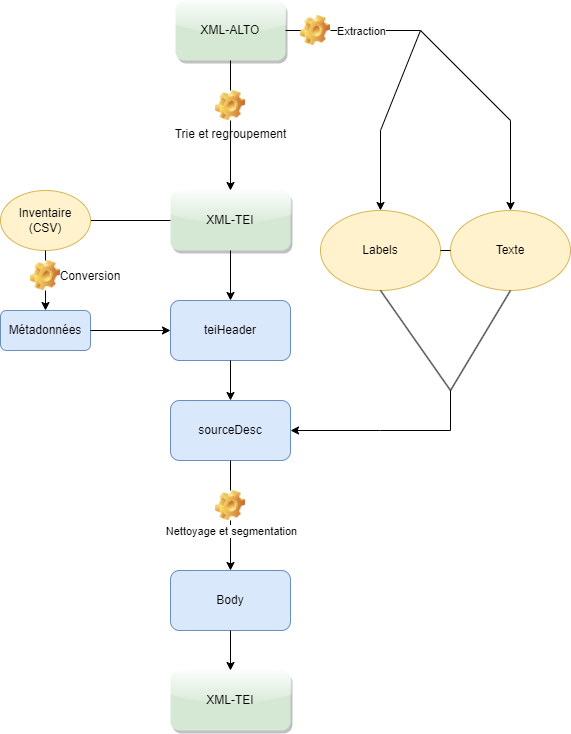
\includegraphics[width=0.7\textwidth]{annexes/schema/altototei.png}
	    \caption{Schéma de conversion des fichiers ALTO vers le format XML-TEI}
	    \label{fig:altototei}
	\end{figure}
	
	Nous avons donc décidé de remanier l'application originale afin d'adopter la structure et la transformation au projet éditorial conçu par le centre \gls{acab}, permettant un gain de temps considérable et fondé sur une une expérience antérieure solide\footnote{application développée pour le projet Araucania est disponible içi. \cite{humeauTeiTransformation2022}}. Comme présenté sur le schéma (voir figure \ref{fig:altototei}), la première étape s'applique à regrouper les fichiers \gls{alto} selon leur identifiant et appliquer la transformation par groupe, en créant la racine \balise{TEI} et de récupérer les labels des régions et des lignes au sein du fichier \gls{alto}. Les différentes métadonnées retranscrites au sein de l'inventaire \gls{csv} sont alors enregistrés au sein du \balise{teiHeader} grâce à la librairie \texttt{Pandas}. Ensuite, le texte contenu dans les \attribut{CONTENT} est extrait des fichiers \gls{alto} et réassocié aux labels précédemment recensés puis structuré selon les pages, les zones puis les lignes au sein du \balise{sourceDesc}. Les données récoltées sont enfin nettoyées et restructurées au sein du \balise{text} en fonction des attributs \attribut{type} et \attribut{subtype} des différentes lignes et des différentes zones afin d'appliquer le schéma éditorial.
	
	\subsection{Documenter et valider un schéma}
	
	Au sein du chapitre 1, nous avons pu constater la variété typologique de notre fonds documentaire et la forte représentativité des sources épistolaires. Pour le moment, le projet c'est avant tout axé sur l'édition de ces documents dont la quantité et la similarité diplomatique justifie une automatisation. Selon l'évolution du traitement du fonds, d'autres schémas pourront être développés.
	
	Afin d'assurer la pérennité de cette édition et le sens sémantique de sa structuration, la conception d'une \gls{ODD} est primordiale puisqu'elle permet de documenter l'ensemble des choix éditoriaux entrepris au cours de cette édition\footnote{La consultation de l'ODD pour la correspondance est consultable au sein du dossier documentation, \cite{humeauTeiTransformation2022}}. Cette documentation devient en quelque sorte le révélateur des enjeux scientifiques, des réflexions éditoriales et de la méthodologie critique du document. Dans notre cas, cette \gls{ODD} à propos de la correspondance a été générée à partir du modèle de transformation \textit{ODD by example} grâce à la création d'un scénario sur le logiciel \texttt{Oxygen} et le processeur Saxon 9. L'\gls{ODD} a par la suite été enrichie manuellement afin de décrire l'encodage utilisé.
	
	\begin{listing}
	        \begin{minted}{xml}
            <constraintSpec scheme="schematron" ident="refVal">
                 <constraint>
                    <s:rule context="tei:placeName[@ref and ancestor::tei:body]">
                        <s:let name="ref" value="@ref"/>
                        <s:assert test="//tei:place[@xml:id = substring-after($ref, '#')] and starts-with($ref, '#')"> The value of @ref has not been declared |<s:value-of select="$ref"/>| </s:assert>
                    </s:rule>
                </constraint>
            </constraintSpec>
            \end{minted}
        	\caption{Application d'une règle \textit{Schematron}}
        	\label{code:schematron}
    \end{listing}
	
	
	
	L'autre enjeu de la construction est la validation et la spécification de notre schéma \gls{tei}. Cette spécification peut se faite grâce aux éléments \balise{schemaSpec}, \balise{moduleRef},\balise{elementSpec} et \balise{classSpec} permettant de modifier la grammaire ou restreindre les règles applicables au schéma \gls{xml}, voir une DTD (Document type definition)\footcite{burnardQuEstceQue2015}. La déclaration de certaines règles \textit{Schematron} a permis de préciser l'usage de certains attributs et de leurs contenus au travers de règles. Comme nous avons pu le voir ci-dessus (voir code \ref{code:schematron}, la règle \textit{Schematron} décrit l'obligation pour tous éléments \balise{placeName} d'avoir son identifiant référencé au sein d'un élément \balise{place} présent au sein du \balise{profileDesc}. La conversion de l'ensemble de ces règles et de cette documentation sous le format \gls{RNG} permet d'automatiser le travail de validation et d'évaluation de la conformité des documents \gls{tei} produits. Cette vérification est exécutée à la fin de l'application du script de conversion avec la fonction de classe \texttt{validate} de la librairie \texttt{lxml}.
	
	\section{Mise en place de l'application autour d'un schéma}
	
	Comme l'amorçait nos premières observations sur l'utilisation d'un script de transformation, la mise en place de cet encodage \gls{tei} nécessite de revenir aux choix employés lors de la production. L'emploi de la libraire \texttt{Lxml} a été indispensable dans l'extraction, la structuration et l'enrichissement des données. 
	
	Ainsi, les axes de nos observations se fondent sur les entités fondamentales de la \gls{tei} : le \balise{teiHeader}, le \balise{sourceDesc} et le \balise{text}.
	
	\subsection{Le teiHeader et ses métadonnées}
	
	Le \balise{teiHeader} correspond à l'élément en-tête d'un fichier XML-TEI. Il regroupe et structure l'ensemble des métadonnées recensées au cours de sa production, permettant d'indexer et de contextualiser le document source. La granularité du schéma des métadonnées doit être ainsi clairement définie en amont en se basant sur la transformation du fichier \gls{alto} lui-même, le ou les documents numériques originelles (facs-similés, ect.) et l'inventaire décrit ultérieurement par la section archivistique du centre \gls{acab}. Le point d'appui pour leurs recensements repose sur l'identifiant extrait du fac-similé numérique afin d'aligner les données avec l'inventaire sous le format \gls{csv}\footcite[voir le fichier ./src/opt/inventory.py ;][]{humeauTeiTransformation2022}.
	
	\begin{figure}[h!]
	    \centering
	    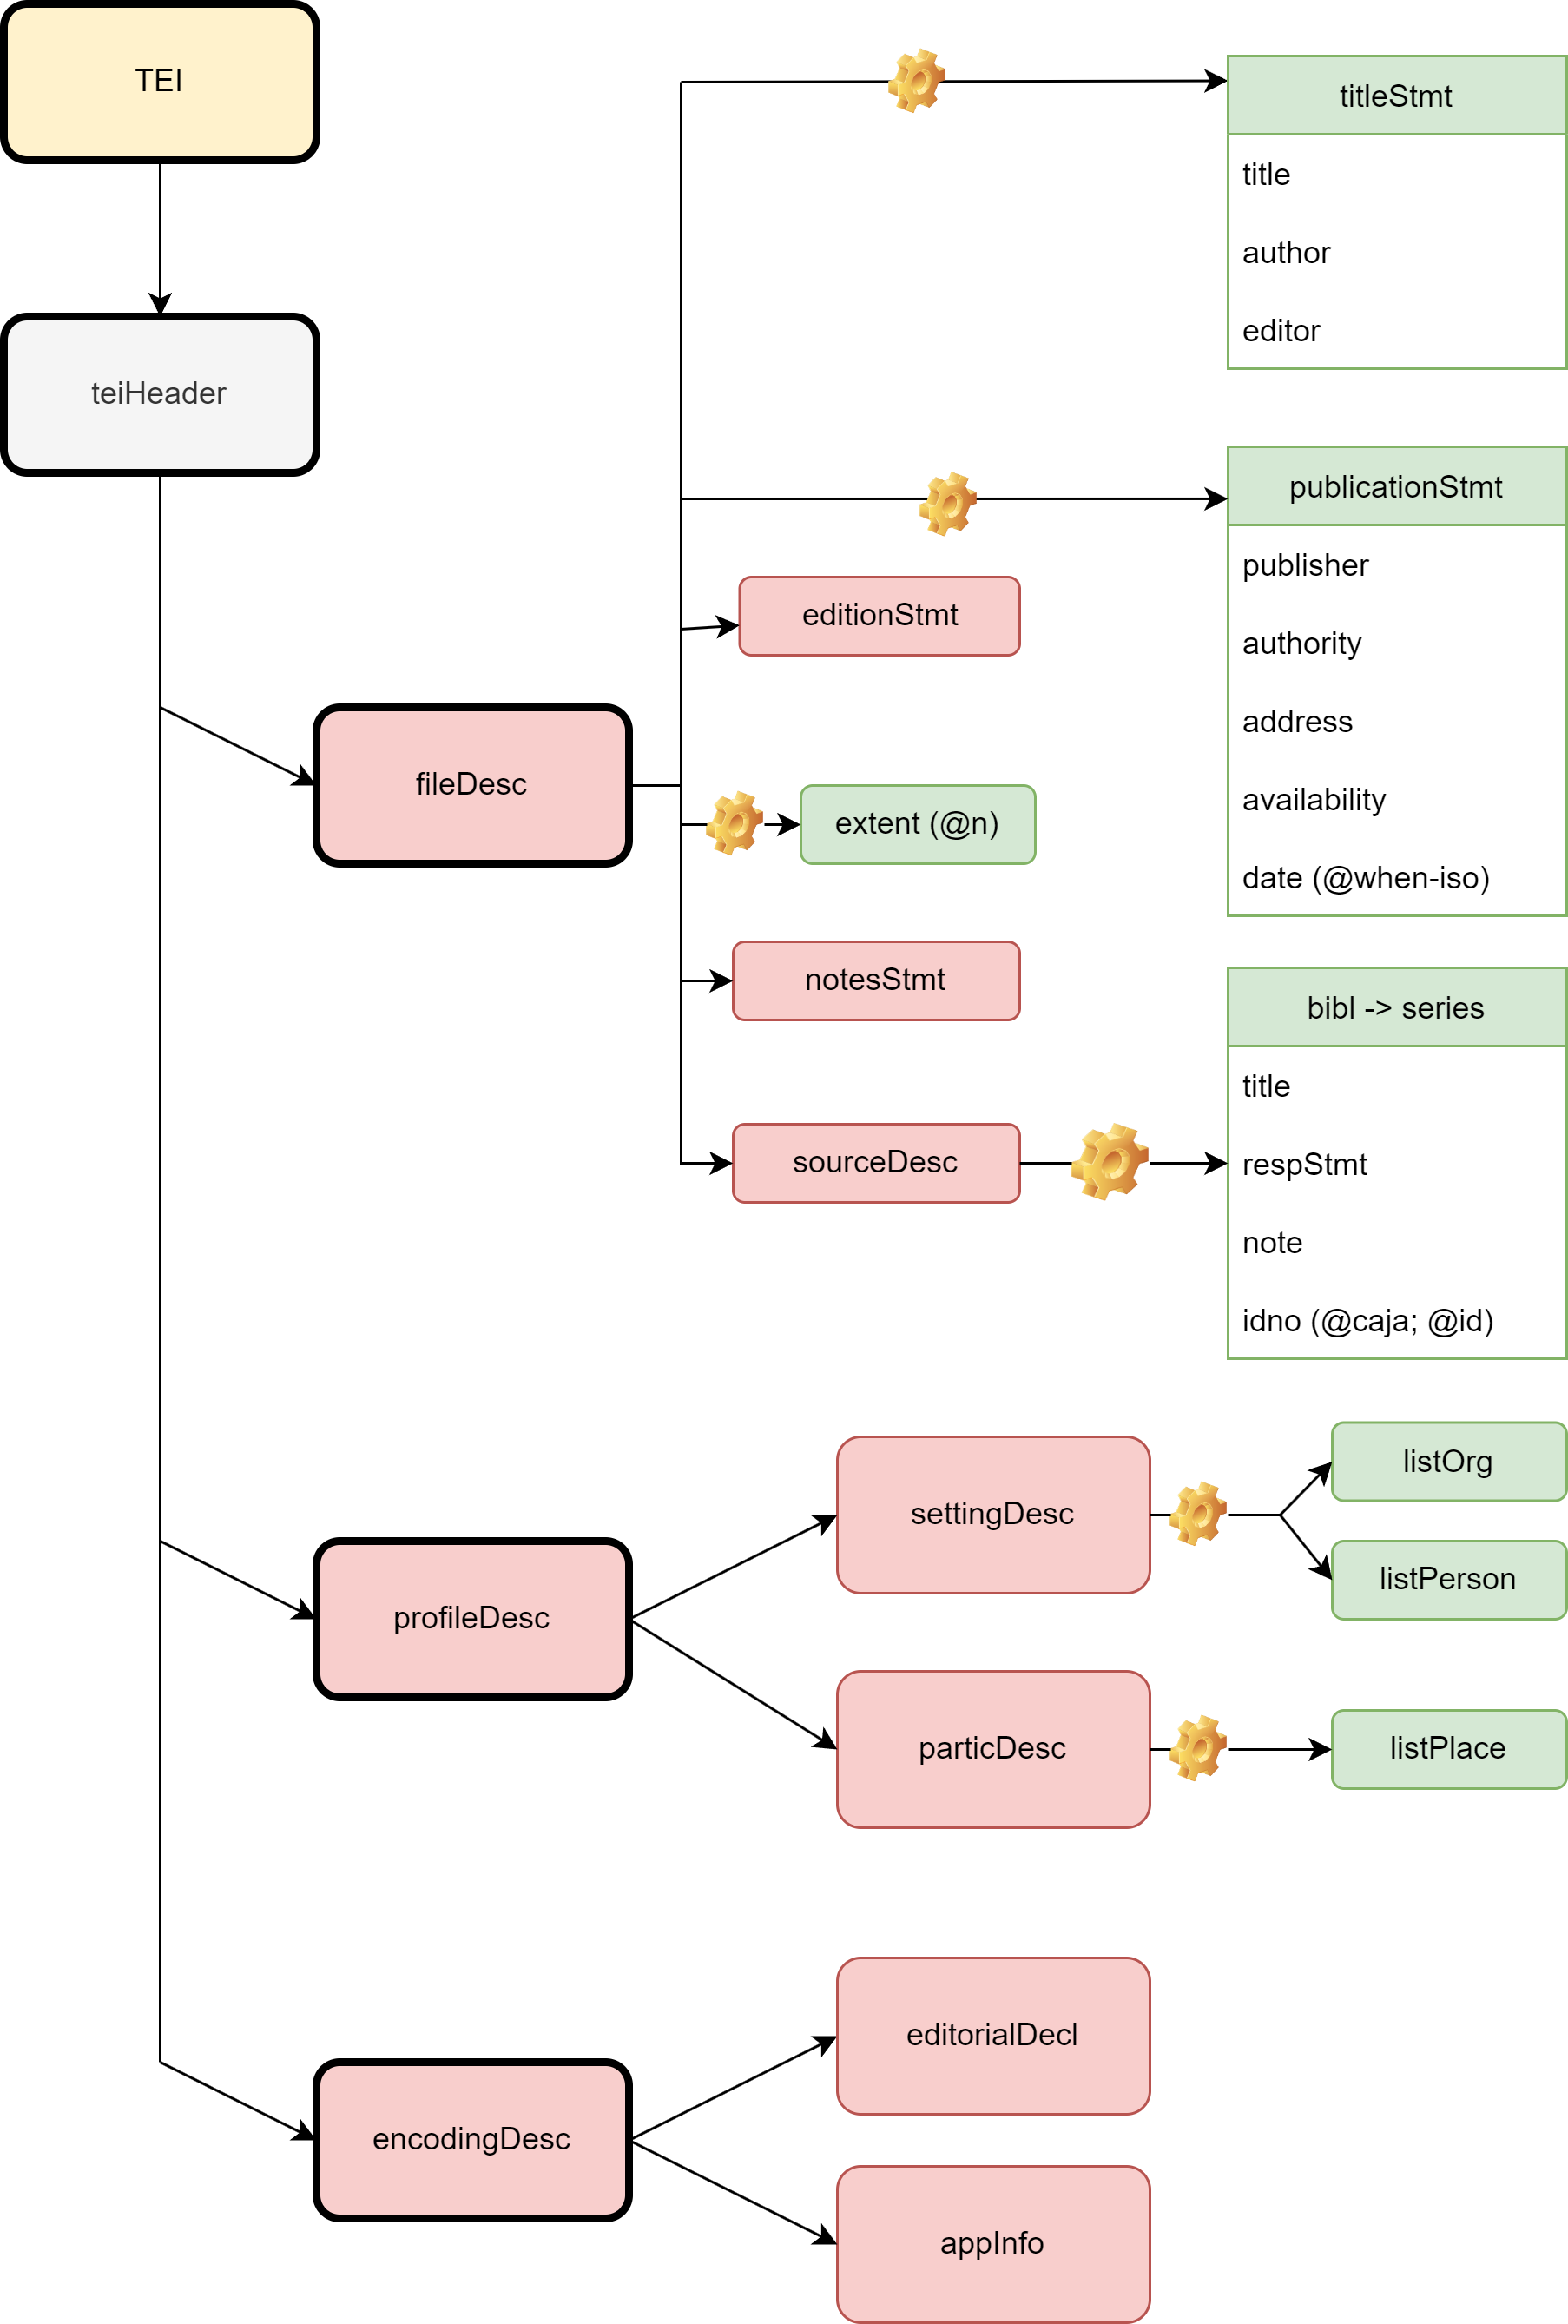
\includegraphics[width=0.7\textwidth]{annexes/schema/teiheader.png}
	    \caption{Structuration du teiHeader}
	    \label{fig:teiheader}
	\end{figure}
	
	Dans un premier temps, les métadonnées décrivent l'ensemble des informations de productions du fichier TEI au sein de l'élément \balise{fileDesc} à partir des métadonnées extraites de l'inventaire\footcite[La structuration de l'arbre du \balise{teiHeader} est disponible en suivant le chemin suivant : ./src/teiheader.py .][]{humeauTeiTransformation2022}. Le \balise{titleStmt} renseigne alors les informations essentielles telles que le titre et l'auteur du document. À l’inverse, les éléments \balise{publicationStmt}, \balise{editionStmt} et \balise{notesStmt} sont pratiquement inamovibles en raison de leur fonction descriptive. Ces balises regroupent les informations de l'autorité éditoriale et de publication. Nous avons choisis de rattacher ces deux éléments à la description du centre \gls{acab} étant, pour le moment, la seule institution véritablement engagée au sein de ce projet d'édition. En revanche, les responsables directs sont identifiables à partir d'un fichier \gls{json} aisément modifiable par les intervenants, puis extrait au cours de la transformation. 
	
	Le décompte des documents rattachés au fichier TEI est décrit au sein de l'élément \balise{extent} affichant la quantité de fac-similés dénombrés sous cet identifiant, avant d'être identifié au sein du \balise{sourceDesc} décrivant le fonds documentaire de l'Araucania. Les métadonnées d'ordre technique sont davantage disposées au sein du \balise{encodingDesc} permettant de décrire succinctement les pratiques autour de cet encodage. L'élément \balise{appinfo} permet de détailler les différentes applications utilisées sur l'ensemble de la chaîne de traitement. Cette description permet de renforcer l'usabilité et la compréhension des données édités en retraçant l'ensemble des processus subit au sein du fichier électronique.

	\subsection{\balise{sourceDoc} : une trace originale}
	
	Dans sa définition officielle, le \balise{sourceDoc} est un élément qui contient une transcription ou autre représentation d'un document source unique faisant potentiellement partie d'un dossier génétique ou d'une collection de sources. Plus concrètement, cet élément devient le lieu de description du fichier \gls{alto} d'origine en reprenant les éléments de mise en page et du texte océrisé. La structuration est directement reprise depuis le modèle établi par l'application \texttt{Alto2tei}\footcite{christensenAlto2tei2022}.
	
	\begin{listing}
	\begin{minted}{xml}
	<surfaceGrp>
      <surface xml:id="299_a" n="16" ulx="0" uly="0" lrx="2327" lry="2970">
        <graphic url="./input/299_a.jpg"/>
        <zone xml:id="299_a_z1" type="CustomZone" subtype="Dateline" n="1" points="1515,217 [...] 1128,178 1294,178 1425,247" source="./input/299_a.jpg" corresp="eSc_textblock_18faefaf">
          <zone xml:id="299_a_z1_l1" type="DefaultLine" subtype="none" n="1" points="1037,388 1133,413 [...] 1034,289 1037,348" source="./input/299_a.jpg" corresp="eSc_line_d13c289a">
            <path xml:id="299_a_z1_l1_p" points="1037,348 [...] 1953,334"/>
            <line xml:id="299_a_z1_l1_t">⁋Valparaiso, Julio 101860</line>
          </zone>
    [...]
    </surface>
    </surfaceGrp>
	\end{minted}
	\caption{Exemple de structuration du sourceDoc}
	\label{code:sourcedoc}
	\end{listing}
	
	En observant plus attentivement, la structuration est une réadaptation du modèle ALTO vers l'encodage TEI en reprenant les données essentielles. L'ensemble des fac-similés numérisés est ainsi décrit au sein de l'élément \balise{surface} en rassemblant l'ensemble des zones et des lignes rattachées. Elles sont décrites au sein de la balise \balise{zone} dont les types et les sous-types issus d'une segmentation préalable indiquent la typologie\footnote{CustomZone:Dateline est décousu en deux attributs : type='CustomZone' et subtype="Dateline")}. L'ensemble des coordonnées ALTO ont été conservées au sein des \attribut{points}, laissant ainsi la possibilité d'exploiter ses coordonnées directement au sein de l'image numérisée. Enfin le contenu textuel est identifiable parmi l'élément \balise{line} et le masque \gls{htr} associé, présent dans l'élément précédent \balise{path}.
	
	La bonne extraction et l'attention particulière à la propreté et la validité des données sont fondamentales puisqu'elles constituent la base de la future structuration du \balise{text}. Du reste, cette conservation exhaustive des données initiales accorde une grande facilité à entretenir l'interopérabilité et la pérennité des éditions numériques, et ainsi leurs réexploitations.
	
	\subsection{Structurer et éditer un texte}
	
	Comme nous l'avons vu au cours du chapitre 1, la définition d'une ontologie et la mise en corrélation avec le vocabulaire contrôle \textit{SegmOnto} au cours du processus de transcription automatique a permis de conserver la valeur sémantique et sémiotique de l'image originale. Cette structuration en amont a ainsi constitué l'arc de voûte de la transformation et l'adaptation de l'\gls{alto} à l'encodage \gls{tei}. À partir de là, l'extraction des différents labels présents au sein du fichier \gls{alto} nous permet d'organiser la structuration du texte en fonction des différentes zones et des différentes lignes présentes.
	
	Au sein de l'élément \balise{text}, il nous faut établir deux subdivisions entre le \balise{body} qui représente le contenu initial du document et le groupe \balise{noteGrp} permettant d'y recenser la plupart des écrits ultérieurs. Seules les lignes contenues au sein d'une zone \textit{NumberingZone} sont référencées au sein de la balise \balise{fw}, à l'intérieur du \balise{body}, indiquant des éléments de mises en pages\footnote{Hormis le sous-groupe \textit{id} qui rejoint les notes postscript}. La seconde étape consiste à repérer le commencement d'une nouvelle page en se référant au numéro de ligne. Si elle est la première, elle indique la présence d'une nouvelle page soulignée par l'incrémentation de l'élément \balise{pb} et son identifiant au sein \attribut{corresp}.
	
	\begin{figure}
	    \centering
	    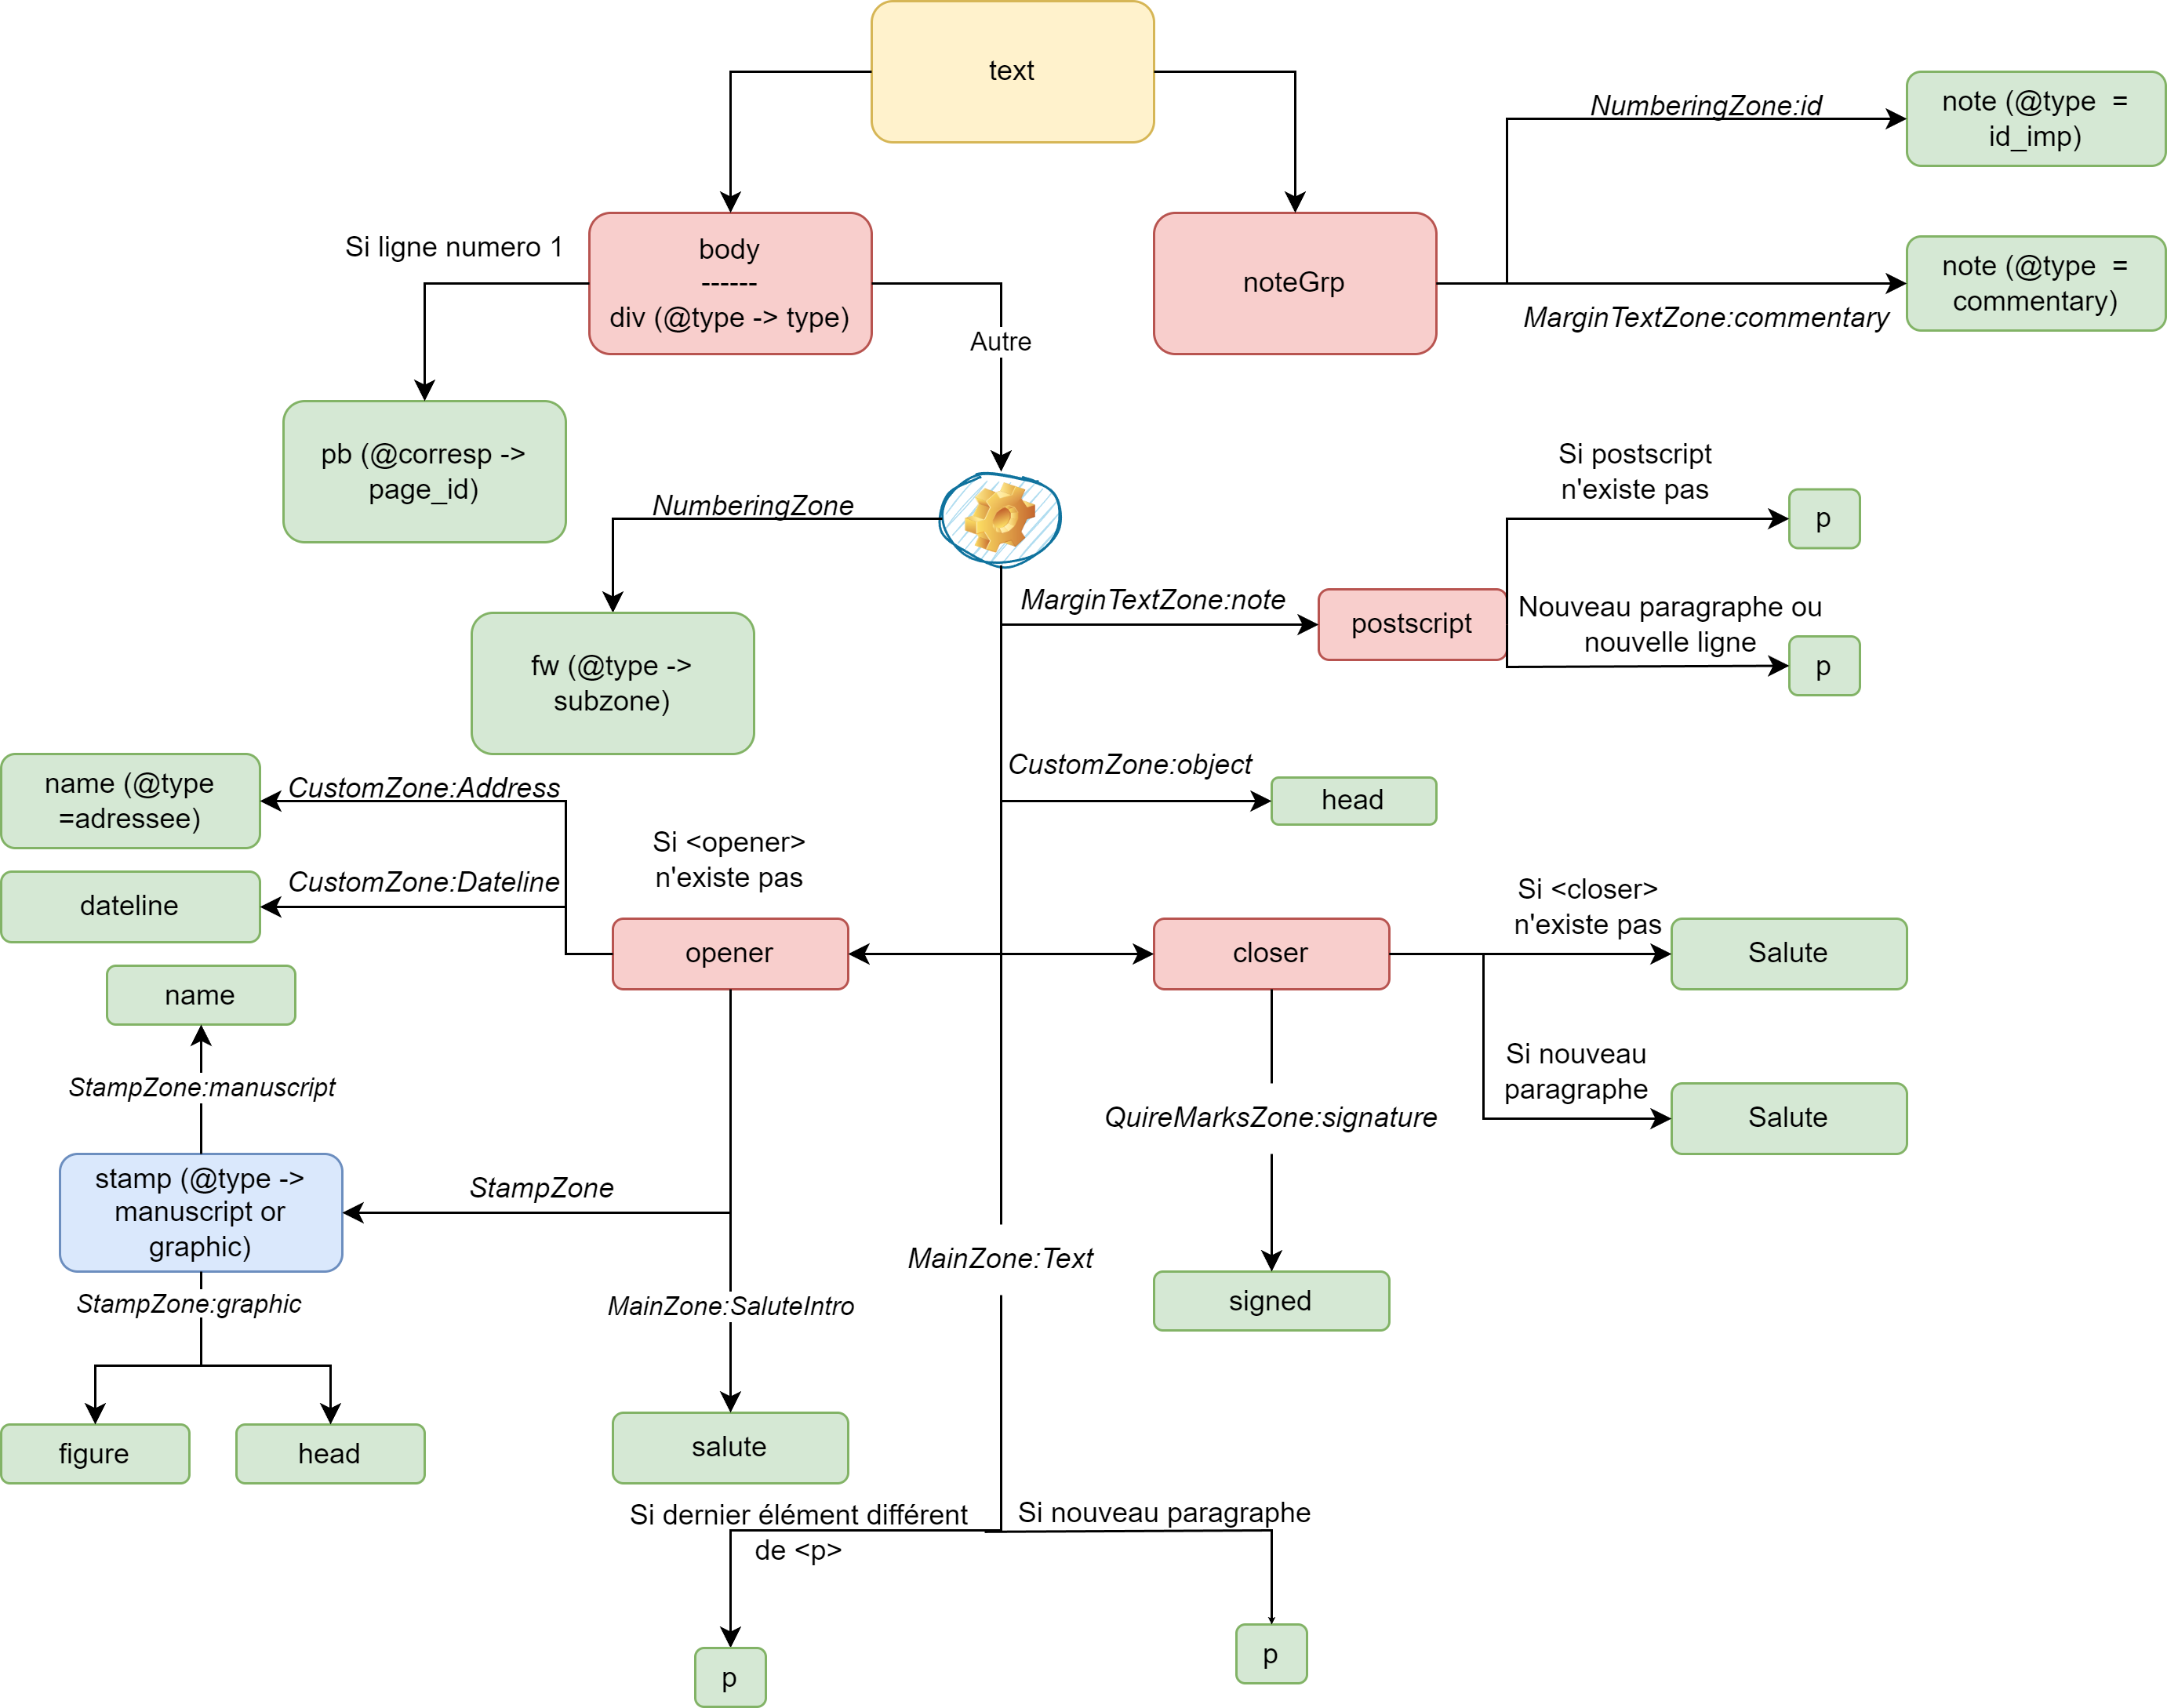
\includegraphics[width=1\textwidth]{annexes/schema/decision_body.png}
	    \caption{Arbre décisionnel de structuration de \balise{text}}
	    \label{fig:arbre_texte}
	\end{figure}
	
	Le schéma et la granularité du \balise{body} sont ainsi organisés en fonction de l'ontologie \gls{htr} développée précédemment. Ce schéma reprend les recommandations du modèle établi pour l'édition de la correspondance de l'édition \gls{dahn}\footcite{chiffoleauDAHNProjectDigital2022}. Ce \balise{body} est en réalité subdivisé en 3 sections majeures et une section optionnelle:
	\begin{itemize}
	    \item \balise{opener} regroupe l'ensemble du discours introductif et les éléments de contextualisation présentés par l'auteur. Il comprend les ontologies \gls{segmonto} suivantes : les éléments \textit{StampZone}, les sous-groupes \textit{CustomZone} comprenant l'adresse, la date (spatiale et temporelle) et la salutation introductive présente au sein du label \textit{MainZone:SaluteIntro}.
	    \item A l'inverse, le \balise{closer} représente l'élément général de conclusion du document. Il rassemble le salut final, parfois sectionné, et la suscription de l'auteur vers son homologue.
	    \item Le corps principal du texte est quant à lui directement injecté au sein du \balise{body} à travers l'élément \balise{p}. Lors de l'énumération des différentes lignes du sourceDoc présentes au sein du \textit{MainZone:text}, la rencontre du signe '\P' signale un nouveau paragraphe qui est alors décompté.
	    \item La mise en place d'un élément \balise{postscript} est parfois nécessaire, en raison de la présence d'une zone possédant le label \textit{MarginTextZone}. Ces notes marginales au texte principal peuvent être divisées en différents paragraphes selon leurs mises en pages. \newline
	\end{itemize}
	
	Cette structuration n'est pas totalement représentative de la mise en page du fac-similé original en raison de la propriété \textit{tail}, mise en place avec la librairie \texttt{Lxml}.  De cette façon, l'\gls{API} \textit{ElementTree} ne nécessite pas de nœuds de texte spéciaux en plus de la classe \textit{Element}, qui ont  parfois tendance à se mettre en travers du chemin. L'inclusion d'une balise autofermante \balise{lb} permet de signaler la présence d'une nouvelle ligne sans déformer la structuration initiale. Cette technique permet de plus facilement ingérer ou modifier le fichier \textit{a posteriori}\footnote{Voir le site web de la librarie Lxml : \textit{Lxml}, url: \url{https://lxml.de/tutorial.html}, consulté le 21/08/2022.}.
	
	Une telle structuration souhaite ainsi répondre aux besoins d'intelligibilité et d'interropérabilité des données éditées comme le rappel l'ingénieur Syd Bauman\footnote{Syd Bauman, \enquote{Interchange vs. Interoperability} In \textit{Balisage: The Markup Conference 2011 Proceedings}, Montréal, 2011 \textit{via} \cite{munozTextsDocumentsNew2014}}. Elle doit faire ressortir aisément les identités du texte à la fois pour l'œil  humain et la machine. L'automatisation de ces éditions renforce ainsi cette accessibilité en facilitant le futur traitement et la future exploitation du fichier TEI édité.
	%%%%%%% CORRECTION DONE %%%%%%%%%%
	
	%%%%%%%%%%%% CHAPTER 4 %%%%%%%%%%%%%%%%%
	\chapter{Indexer et enrichir une édition numérique}
	
	Alors que les humanités numériques, évoquées au travers de la philologie, incarnent un progrès méthodologique considérable pour le travail en amont, Jean-Baptiste Camps rappelle que cette mise en place d' une édition numérique reste un effort fastidieux, chronophage et coûteux pour les institutions\footcite{campsOuVaPhilologie2018}. Si la sérialisation des données ne peut-être une fin en soi, l'enrichissement des textes, primordial à la recherche, peut tout de même être considérablement allégé grâce à l'ingénierie.
	
	Aujourd'hui, les outils associés au traitement automatique des langues sont devenus suffisamment matures et fiables pour fournir une analyse à la fois quantitative et qualitative. Ces avancées ont permis de créer un véritable engoument du \gls{tal} au sein des humanités numériques et de l'édition numérique\footcite{mcgillivrayDigitalHumanitiesNatural2020}. De nombreux écosystèmes ont été développés dans le but de permettre un enrichissement quantitatif de bases de données XML-TEI à partir de la fouille de texte et l'extraction de l'information\footcite{bissonNoticesAutoriteXMLTEI2020}. Ces différents processus permettent régulièrement la correction des données produites par les modèles \gls{htr}\footnote{Nous l'avons partiellement vu avec la mise en place d'une application correctrice au travers de l'algorithme de Levenshtein}, l'indexation des entités ou encore de faciliter la recherche au sein du texte\footcite{terrielRepresenterEvaluerDonnees2020}.
	
	Durant ce projet d'édition des archives de l'Occupation de l'Araucania, l'implantation d'un système d'enrichissement fondé sur les concepts du traitement automatique du langage et la reconnaissance d’entités nommées a été un des axes majeurs du processus éditorial. La mise en place d'un tel procédé nécessite de revenir sur les enjeux épistémologiques et techniques d'un processus lourd et complexe. Dans ce cadre, nous allons observer au cours de ce chapitre les différentes réflexions et observations qui ont accompagné et nourrie cette insertion technique d'un pré-enrichissement automatique.
	
	
	\section{L'ébullition du traitement du langage naturel}
	
	Pour comprendre les progrès qui ont entouré l'incorporation du \gls{tal} dans le domaine des humanités numériques, il est nécessaire d'en décliner les principes généraux et les innovations récentes permises par la généralisation du \textit{deep learning} et des nouvelles architectures affiliés.
	
	En ce sens cette partie se veut comme un aparté pédagogique et introductif autant sur le plan théorique que technique.
	
	\subsection{Principes généraux du TAL}
	
	Le traitement automatique des langues est en réalité une discipline regroupant un ensemble de pratiques autour de l'analyse et l'interprétation des langues naturelles à travers l'outil informatique. Ce domaine pluridisciplinaire est ainsi à la croisée de la linguistique, de l’informatique, des mathématiques et de l’intelligence artificielle. Aujourd'hui, le \gls{tal} regroupe un ensemble de technologies de la vie courante et scientifique tel que les traducteurs automatiques, l'analyse marketing et des sentiments, le \textit{data mining} (fouille de texte, en français), la correction orthographique, la reconnaissance vocale, etc... Quatre catégories peuvent être définies : le traitement syntaxique et sémantique, l'extraction d'information et le traitement du signal\footnote{Cette catégorisation reprend la déclinaison faite au sein de la page Wikipedia dédiée au \gls{tal}. \textit{Wikipidia | Traitement automatique des langues}, url: \url{https://fr.wikipedia.org/wiki/Traitement_automatique_des_langues}, consulté le 20/08/2022.}.
	
	Le \gls{tal} provient d'un très long processus de recherche remontant aux débuts des années 1960 avec un véritable engouement probabiliste à partir des années 1983 et 1984\footcite[Cette éclosion d'intérêt au sein des milieux scientifiques est permis avec la publication des premiers arbres de décisions et de d'un système d'étiquetage probabiliste.][]{tanguyEvolutionsLinguistiqueOutillee2014}. Dans un article paru en 2014, Ludovic Tanguy y distingue deux méthodes : la première dite \enquote{traditionnelle} ou linguistique consistant à formaliser les règles à appliquer et les ressources linguistiques. La seconde réside dans la mise en place de modèles mathématiques et statistiques applicables à l'intelligence artificielle\footcite{tanguyEvolutionsLinguistiqueOutillee2014}.
	
	À l’heure actuelle, ce domaine de l'apprentissage machine s'appuie sur un ensemble de pratiques syntaxo-sémantiques bien précises, bâtit autour des modèles linguistiques, dont les principales fonctionnalités sont les suivantes :
	\begin{itemize}
	    \item La tokenisation qui consiste en la segmentation d'une phrase en mot ou d'un mot en caractères.
	    \item Le \textit{stemming} et la lemmatisation. La première technique désigne le découpage de la fin du mot pour en conserver la racine. La lemmatisation consiste quant à elle à supprimer les terminaisons \enquote{en isolant la forme canonique du mot\footcite{labbeNormalisationLemmatisationQuestion}}.
	    \item L’étiquetage morpho-syntaxique (POS) est un processus reliant le mot à sa fonction grammaticale.
	    \item La suppression des mots vides (\textit{stop words} en anglais), c’est-à-dire les mots courants et vides de sens propres.
	    \item Le Plongement de mots ou lexical (\textit{word embbeding} en anglais) est une méthode de représentation d'un mot sous forme de vecteur. Elle donne une valeur numérique au sens et au contexte du mot en établissant un vecteur contextuel.
	\end{itemize}
	
	\subsection{Les réseaux neuronaux et le TAL : la révolution des modèles encodeurs-decodeurs}
	
	Aujourd'hui, le \gls{tal} s'est totalement inséré dans nos vies quotidiennes avec la renaissance du \textit{machine learning}, après la crise qu'il a connu au cours des années 2000. Plus particulièrement, cette démocratisation a été permise par l'amélioration notable des performances avec l'utilisation du \textit{deep learning}. Ces dernières avancées ont su puiser dans l'approche du \textit{Word Embbeding} afin de constituer des algorithmes statiques au texte à l'image du système \textit{Word2Vec}, notamment le modèle Skip-Gram\footcite[D'autres valorisent des approches moins lourdes de plongement de mots tel que le \textit{Singular Value Decomposition}][]{moodyStopUsingWord2vec2017}. 
	
	En 1957, le linguiste John Rupert Firth émet l'hypothèse suivante : \enquote{You shall know a word by the compagny it keeps !\footnote{\enquote{Vous reconnaîtrez un mot à la compagnie qu'il garde !} in \cite{widdowsonFirth1957Papers2007}}}. Cette hypothèse distributionnelle qui reconnaît un mot à partir de son contexte va être le socle du système \textit{Word2Vec}. Alors, l'algorithme de transformation vers des valeurs algébriques tend à étendre la définition originale de la distribution en y incluant une valeur sémantique et contextuelle au travers d'espaces multidimensionnels. La distance vectorielle indique ainsi la proximité sémantique entre deux mots. Ces transformations des mots sous des modèles algébriques (matriciels et vectoriels) permettent ainsi de définir les poids des réseaux neuronaux appliqués.
	
	\begin{figure}[h!]
	    \centering
	    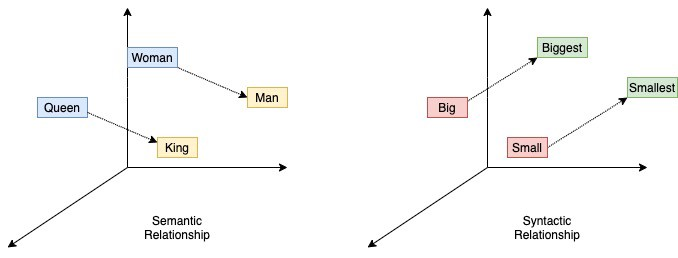
\includegraphics[width = 0.7\textwidth]{annexes/img/word_embedding.jpeg}
	    \caption{Représentation vectorielle des relations sémantiques et syntaxiques - \copyright towardsdatascience, 2021}
	    \label{fig:word_embedding}
	\end{figure}
	
	Afin de traiter les données en séries, deux architectures neuronales sont principalement utilisés; les premiers furent les réseaux neuronaux acycliques (RNN ; LSTM et GRU), aujourd'hui dépassés en raison des problèmes de \enquote{rétropropagation}\footcite[p.~161]{clericeDetectionIsotopiesPar2022}. C'est-à-dire que l'algorithme concentre davantage son attention sur la fin d'un élément. Ce phénomène est réglé par les réseaux \gls{CNN} en prenant l'élément dans sa globalité\footcite[p.~164]{clericeDetectionIsotopiesPar2022}. Ce réseau s'exerce en deux étapes : la partie convolutive qui se tâche de l'extraction des caractéristiques propres à travers différents algorithmes de transformation (\textit{pooling}, échantillonage, etc...), puis la classification des données.
	
	Depuis la fin des années 2010, le \gls{tal} s'est dirigé vers les architectures encodeurs-décodeurs. Cette innovation se fonde sur les réseaux acyliques et l'application du mécanisme de l'attention, du système \textit{Masked LM}, l'application d'un masque aléatoire permettant une approche simultanée du traitement, et l'approche du \textit{Dynamic Embedding}\footcite{vaswaniAttentionAllYou2017}. En 2018, Google présente le modèle BERT (\textit{Bidirectional Encoder Representations from Transformers}) qui étalonne en de multiples étapes cycliques le traitement textuel \textit{via} une architecture encodeur-décodeur\footcite{devlinBERTPretrainingDeep2019a}. Ces modèles de langage appellent plus couramment appelés modèles \textit{Transformers}. Ces modèles de langages sont des outils de pré-entraînement de modèles plus perfectionnés, à travers la méthode du \textit{fine-tuning}.
	
	De nombreux modèles de langage ont fait leurs apparitions à la suite de cette révolution au sein du \gls{tal} et la démocratisation des modèles \textit{Transformers}\footnote{Il est à noter que cette architecture démontre aussi des capacités prometteuses pour le cas de la reconnaissance d'écriture. \cite{kassAttentionHTRHandwrittenText2022}}. En 2020, l'Universidad de Chile développe et publie le modèle BETO qui reprend les principes de cette architecture pour l'adapter à la langue espagnole, en utilisant la méthode du \textit{fine-tuning} avec le modèle BERT \footcite{caneteSpanishPreTrainedBERT2020}. Le \textit{dataset} a été constitué à partir des données de Wikipedia et du projet OPUS. Comme l'indique le tableau \ref{tab:beto_benchmarlk}, les résultats du modèle sont très satisfaisants, plus particulièrement pour le modèle prenant en compte la case dans son analyse. Ce modèle constituera notre point d'appui pour le développement du projet d'enrichissement de nos éditions numériques.
	
    \begin{table}[]
    \begin{tabular}{|c|r|r|r|}
    \hline
    \textbf{TASK} & \multicolumn{1}{c|}{\href{https://huggingface.co/dccuchile/bert-base-spanish-wwm-cased}{\textbf{BETO-cased}}} & \multicolumn{1}{c|}{\href{https://huggingface.co/dccuchile/bert-base-spanish-wwm-uncased}{\textbf{BETO-uncased}}} & \multicolumn{1}{c|}{\href{https://huggingface.co/bert-base-uncased}{\textbf{Best Multilingual BERT}}} \\ \hline
    \href{https://lindat.mff.cuni.cz/repository/xmlui/handle/11234/1-1827}{POS}           & 98.97                                    & 98.44                                      & 97.10                                                \\ \cline{1-1}
    \href{https://www.kaggle.com/datasets/nltkdata/conll-corpora}{NER-C}         & 55.43                                    & 82.67                                      & 87.38                                                \\ \cline{1-1}
    \href{https://github.com/facebookresearch/MLDoc}{MLDoc}         & 95.60                                    & 96.12                                      & 95.70                                                \\ \cline{1-1}
    \href{https://github.com/google-research-datasets/paws/tree/master/pawsx}{PAWS-X}        & 89.05                                    & 89.55                                      & 90.70                                                \\ \cline{1-1}
    \href{https://github.com/facebookresearch/XNLI}{XNLI}          & 82.01                                    & 80.15                                      & 78.50                                                \\ \cline{1-1} \hline
    \end{tabular}
    \caption{Évaluation des performances du modèle BETO (selon standard GLUE)}
    \label{tab:beto_benchmarlk}
    \end{table}
	
    \subsection{Le TAL, la reconnaissance des entités nommées et les humanités}
    
    L'extraction d'information est une catégorie générale de la linguistique computationnelle dont le principe repose sur l'analyse, une sélection et une classification pertinentes d'une donnée textuelle\footcite{poibeauExtractionInformationNouvelle1999}. Elle regroupe de nombreuses tâches permettant de déstructurer et reconstruire l'information telle que l'identification des relations et des évènements, l'extraction de propriétés, la résolution des coréférences ou dans ce qui nous concerne, la reconnaissance des entités nommées.
    
    Le concept linguistique des entités nommées définit le principe d'une classification des mots selon son fonctionnement référentiel. Dans sa thèse sur les processus d'extractions des entités nommées, Maud Ehrmann les décrit comme \enquote{Étant donné un modèle applicatif et un corpus, on appelle entité nommée toute expression linguistique qui réfère à une entité unique du modèle de manière autonome dans le corpus.\footcite[p.~167-168]{ehrmannEntiteesNommeesLinguistique2008}}. Cette définition décrit des propriétés malléables dépendantes d'une ontologie définie préalablement, dont la référence sémantique est alors primordiale et la référence syntaxique secondaire (exemple : les noms propres). Autrement dit, la nature d'une entité nommée ne réside pas dans son essence, mais bien dans son existence applicative\footcite[p.~167-168]{ehrmannEntiteesNommeesLinguistique2008}.
    
    \begin{figure}
        \centering
        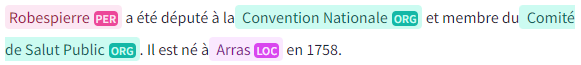
\includegraphics[width=0.6\textwidth]{annexes/img/entites.png}
        \caption{Exemple de reconnaissance d'entités nommées à partir du modèle camemBERT}
        \label{fig:entités}
    \end{figure}
    
    Comme le présente la figure \ref{fig:entités}, la reconnaissance d'entités nommées est une technique consistant à repérer ces chaînes de caractères au sein d'un texte et d'en déterminer son référentiel. Ici, l'ontologie employée se décline en quatre grandes natures : \texttt{LOC} pour les lieux géographiques, \texttt{ORG} pour les organisations, \texttt{PERS} pour les personnes et \texttt{MISC} pour les entités diverses et regroupées au sein de cette catégorie générale (non référencée dans notre cas). Cette approche de classification est parmi les plus communes puisqu'elle reprend les règles définit par CoNLL 2003, une conférence annuelle organisée par la SIGNLL (\textit{ACL's Special Interest Group on Natural Language Learning})\footcite{lemmensCoNLL2022CoNLL2022}. Toutefois, cette normalisation ne peut faire l'objet d'un véritable consensus puisque l'étiquetage reste dépendant des sujets traités en prenant en compte les limites, la porté et la granuralité d'une entité\footcite{hengchenExtractionEntitesNommees2015}.
    
    \subsubsection{Les techniques de reconnaissances des entités nommées}
    
    Le processus de reconnaissance des entités nommées peut s'exercer à travers deux approches techniques, non nécessairement dichotomiques. La première est l'étiquetage des entités par l'intervention humaine en définissant des règles appliquées à partir d'une ontologie préalable. 
    
    Cette méthode majoritairement répandue dans les années 1990 est décrite comme la mise en forme de \enquote{patrons d'extraction} en exploitant les indices morpho-syntaxique et un ensemble de ressources externes\footcite[p.~32]{ehrmannEntiteesNommeesLinguistique2008}. Pour reprendre l'exemple de Maud Ehrmann, si Maximilien est un nom connu au sein des ressources utilisées et que le nom suivant Robespierre est inconnu, mais qu'il possède une majuscule et suit la première entité; alors l'approche statistique peut facilement déduire que Robespierre appartient à l'entité \texttt{PERS}\footcite[p.~33]{ehrmannEntiteesNommeesLinguistique2008}. Toutefois, la mise en place de motifs probabilistes reste parfois insuffisant en raison d'un paramétrage intrinsèquement trop large comme le signale Damien Nouvel\footcite[p.~146]{nouvelReconnaissanceEntitesNommees2012}.
    
    Cette approche a été confortée avec l'utilisation de l'intelligence artificielle qui connaît un nouveau souffle après les années 2000. Elle nécessite l'emploi d'une base de données afin de pouvoir y entraîner différents modèles. Parmi les approches courantes, on peut y recenser :
    \begin{itemize}
        \item L'apprentissage non-supervisé en utilisant des techniques de \textit{clustering}, c'est-à-dire de regroupement de données selon une interprétation machine\footcite{liSurveyDeepLearning2020}.
        \item L'apprentissage supervisé, utilisant donc des données préalablement étiquetées dont les principaux algorithmes utilisés sont les arbres de décisions, le \textit{Machine Support Vector} (SVM) ou le système Markov caché\footcite{liSurveyDeepLearning2020}. Ces modèles sont assez similaires aux modèles classiques de \gls{htr}.
        \item Les algorithmes d'apprentissages profonds se sont imposés comme l'architecture dominante depuis ces dernières années dans les taches de reconnaissances d'entités nommées\footcite{liSurveyDeepLearning2020}. L'ébullition des architectures \textit{Transformers} a amplifié ce phénomène en raison de ces résultats (voir tableau \ref{tab:beto_benchmarlk}). De plus, l'apprentissage profond permet de traiter facilement des données complexes et l'obtention d'un modèle multi-tâche, facilement intégrable au sein d'une chaîne de traitement.
    \end{itemize}
    
    \subsubsection{La REN et les humanités}
    
    L'intégration des technologies \gls{ren} a susciter de nombreux émois au sein des secteurs patrimoniaux et des humanités. La place de plus en plus grande qu'occupent les humanités numériques au sein de la recherche a multiplié l'intérêt pour cette tâche. La préparation de données statiques ou le renouveau historiographique permis par la méthode de \textit{Distant reading}\footnote{Méthode d'analyse historique imaginé par Franco Moretti. Elle consiste en l'application des méthodes calculs et d'observations de motifs à l'échelle de grandes bases de données. \cite{purenLectureDistanteIntroduction2020a}} ont généralisée la fouille de texte, dont l'extraction des entités nommées permet une annotation efficace des documents.
    
    Dans le même temps, le catalogage et l’indexation manuel sont mis à rude épreuve depuis plusieurs années en raison des restrictions budgétaires au sein des secteurs culturels et la multiplication des documents archivés\footcite{hengchenExtractionEntitesNommees2015}. Face à ce constat, les institutions patrimoniales s'essayent à réoganiser le processus d'indexation avec une utilisation systémique des technologies \gls{ren}. Le projet NER4Archives développés par les Archives Nationales en partenariat avec l'\gls{inria} démontre cette volonté d'automatiser la classification au sein des instruments de recherche archivistique\footcite{clavaudNER4ArchivesNamedEntity2022}.
    
    La volonté d'incorporer cette tâche de classification de l'information n'est pas nouvelle et s'appuie sur de nombreuses expériences antérieures d'application sur les documents historiques, notamment au sein d'une chaîne de traitement d'océrisation. Les modèles \textit{Tranformers} ont démontré une certaine capacité dans le traitement et l'extraction des informations au sein de corpus numérisés bruyants sans pour autant en dégrader les performances\footcite{borosAlleviatingDigitizationErrors2020}. En 2020, Manuel Carbonell et Al. vont encore plus loin et démontrent la capacité d'amélioration de la reconnaissance de caractères manuscrits au sein d'un modèle unifié avec la reconnaissance d'entités nommées et la localisation de texte\footcite{carbonellNeuralModelText2020}. Dans notre cas, plusieurs projets ont intégré l'automatisation de la \gls{ren} au sein des chaînes de traitements d'éditions numériques à l'image des projets AGODA (Analyse sémantique et Graphes relationnels pour l’Ouverture et l’étude des Débats à l'Assemblée nationale) ou encore le \gls{lectaurep}\footcite{bourgeoisUsingTopicGeneration2022, scheithauerReconnaissanceEntitesNommees2021}.
    
    Ces différents constats prometteurs, nous amenés à considérer et évaluer l'intégration de la \gls{ren} au cours de l'édition du corpus autour de l'Occupation de l'Araucanie.
	
	\section{Entraîner la reconnaissance d'entités nommées}
	
	Face au constat de la difficile adaptation des modèles \gls{ren} généralistes sur les données océrisées d'un espagnol latino-américain du XIX\textsuperscript{e} siècle\footnote{Différents modèles (BETO, Flair) ont été expérimentés sur des vérités terrains via l'interface HuggingFace.}, il a été rapidement décidé d'expérimenter la mise en place d'un modèle propre au projet et d'enrichir l'annotation. Néanmoins, ce choix ne peut être éffectué sans prendre en considération le coût humain, mais aussi énergétique et écologique que représente la génération d'un modèle \textit{Transformers}. La prise de conscience de cet aspect est une nécessité face à la massification des modèles et méga-modèles \gls{tal} et de \textit{machine learning} dans leur globalité\footcite{strubellEnergyPolicyConsiderations2019}.
	
	À travers cette aspiration, nous allons observer comment peut on développer un modèle \gls{ren} et les enjeux qui ont entouré la production des données et l'apprentissage.
    
    \subsection{Annoter un jeu de données pour la reconnaissance d'entités nommées}
    
    Le développement d'un modèle de reconnaissance \gls{ren} est le fruit d'un long processus d'annotation des entités à partir d'un corpus de données. La mise en place d'un système de reconnaissance d'entités nommées à partir de documents historiques rencontre trois défis majeurs selon une étude dirigée par Maud Erhmann et al.\footcite{ehrmannNamedEntityRecognition2021}. Le premier est ce qu'on appelle la \enquote{dynamique de langues} c'est-à-dire la prise en compte des variations orthographiques historiques (et du niveau de langue dans notre cas), les conventions de noms ou encore les entités contextuelles dont le sens évolue à travers le temps. Les autres points de difficultés sont la gestion des espaces, notamment pour les documents historiques médiévaux, et la gestion du bruit suite aux procédés de reconnaissances \gls{htr}. Dans de nombreux cas, il est possible de s'appuyer sur des corpus annotés existant au sein d'un \enquote{lac de ressources} afin d'adapter des modèles ayant déjà fait leur preuve. Néanmoins, la langue espagnole n'est présente que marginalement et ne peut pas répondre à nos besoins spécifiques\footcite[Seul un corpus de transcriptions médiévales espagnols et un jeu concernant des données bibliographiques multilingues ont été identifiés.][]{ehrmannNamedEntityRecognition2021}. Les données de vérité terrain ont été directement reprises de notre jeu utilisé pour l'entraînement d'un modèle \gls{htr}. 
    
    Afin de saisir notre jeu de données final, il nous faut préalablement revenir sur le protocole d'annotations et le pré-traitement des données \gls{alto}. Tout d'abord, les transcriptions ont été nettoyées des méthodes utilisées pour la transformation du format \gls{alto} vers le format \gls{tei} avec l'utilisation de \gls{regex}, avant d'être converti sous le format texte qui définit comme notre standard de donnée. Le pré-traitement est volontairement minimaliste, car l'objectif de ce modèle est d'être capable d'analyser correctement à partir de données bruitées issues de la \gls{rem}. Il doit être capable de poursuivre son analyse au-delà des dynamiques de langues ou des erreurs d'océrisations, malgré un impact minimal. Confirmant les premières constatations observées lors de la conférence \textit{24th Conference on Computational Natural Language Learning}\footcite{borosAlleviatingDigitizationErrors2020}, Les expériences de Hugo Scheithauer au sein du projet \gls{lectaurep} démontrent l'impact très relatif du \gls{CER} sur les performances des modèles \gls{tal} en dessous de 20\%\footcite[p.~102-104]{scheithauerReconnaissanceEntitesNommees2021}. Le point primordial est donc de former à la compréhension des abréviations et la segmentation de certaines entités, notamment à la suite de saut de ligne. \newpar
    
    Par la suite, nous avons établi un protocole d'annotation à la fois concernant l'ontologie à appliquer et le processus. Pour ce dernier, nous avons donc établi qu'une première personne effectue une annotation avant d'être vérifiée par une seconde personne afin d'obtenir un consensus sur les étiquetages ambigus.
    Certaines initiatives scientifiques ont publié certains schémas possibles en fonction de la nature du référentiel. En reprenant certaines recommandations du Manuel d’annotation linguistique publié par les chercheurs Simon Gabay et al.\footcite{gabayManuelAnnotationLinguistique2022}, nous avons établi 5 groupes d'entités selon les conditions suivantes :
    \begin{itemize}
        \item LOC -- Lieux géographiques ou administratifs (564 entités annotées)
        \item ORG -- Organisations administratives et institutionnelles (398 entités annotées)
        \item PERS -- Personne ou groupes de personnes (1022 entités annotées)
        \item DATE -- Dates absolues ou relatives, voir événement (262 entités annotées)
        \item MISC -- Entités d'intérêts et inclassables au sein des référentiels précédents: navires, objets de ravitaillements, stratégies, etc... (430 entités annotées)
    \end{itemize}
    
    L'entité MISC est volontairement englobante et peu précise. L'intention était d'observer la capacité d'identification d'éléments plus précis notamment le ravitaillement (PROD) ou encore les bateaux à vapeur dont les premières hypothèses appuient l'utilisation d'un sous-groupe à ORG ou l'ajout d'une entité propre (BAT par exemple). Souvent un compromis doit-être fait entre précision et simplification afin d'améliorer la performance du modèle et la capacité d'extraction de données\footcite{grouinSimplificationSchemasAnnotation2018}. 
    
    \begin{figure}[h!]
        \centering
        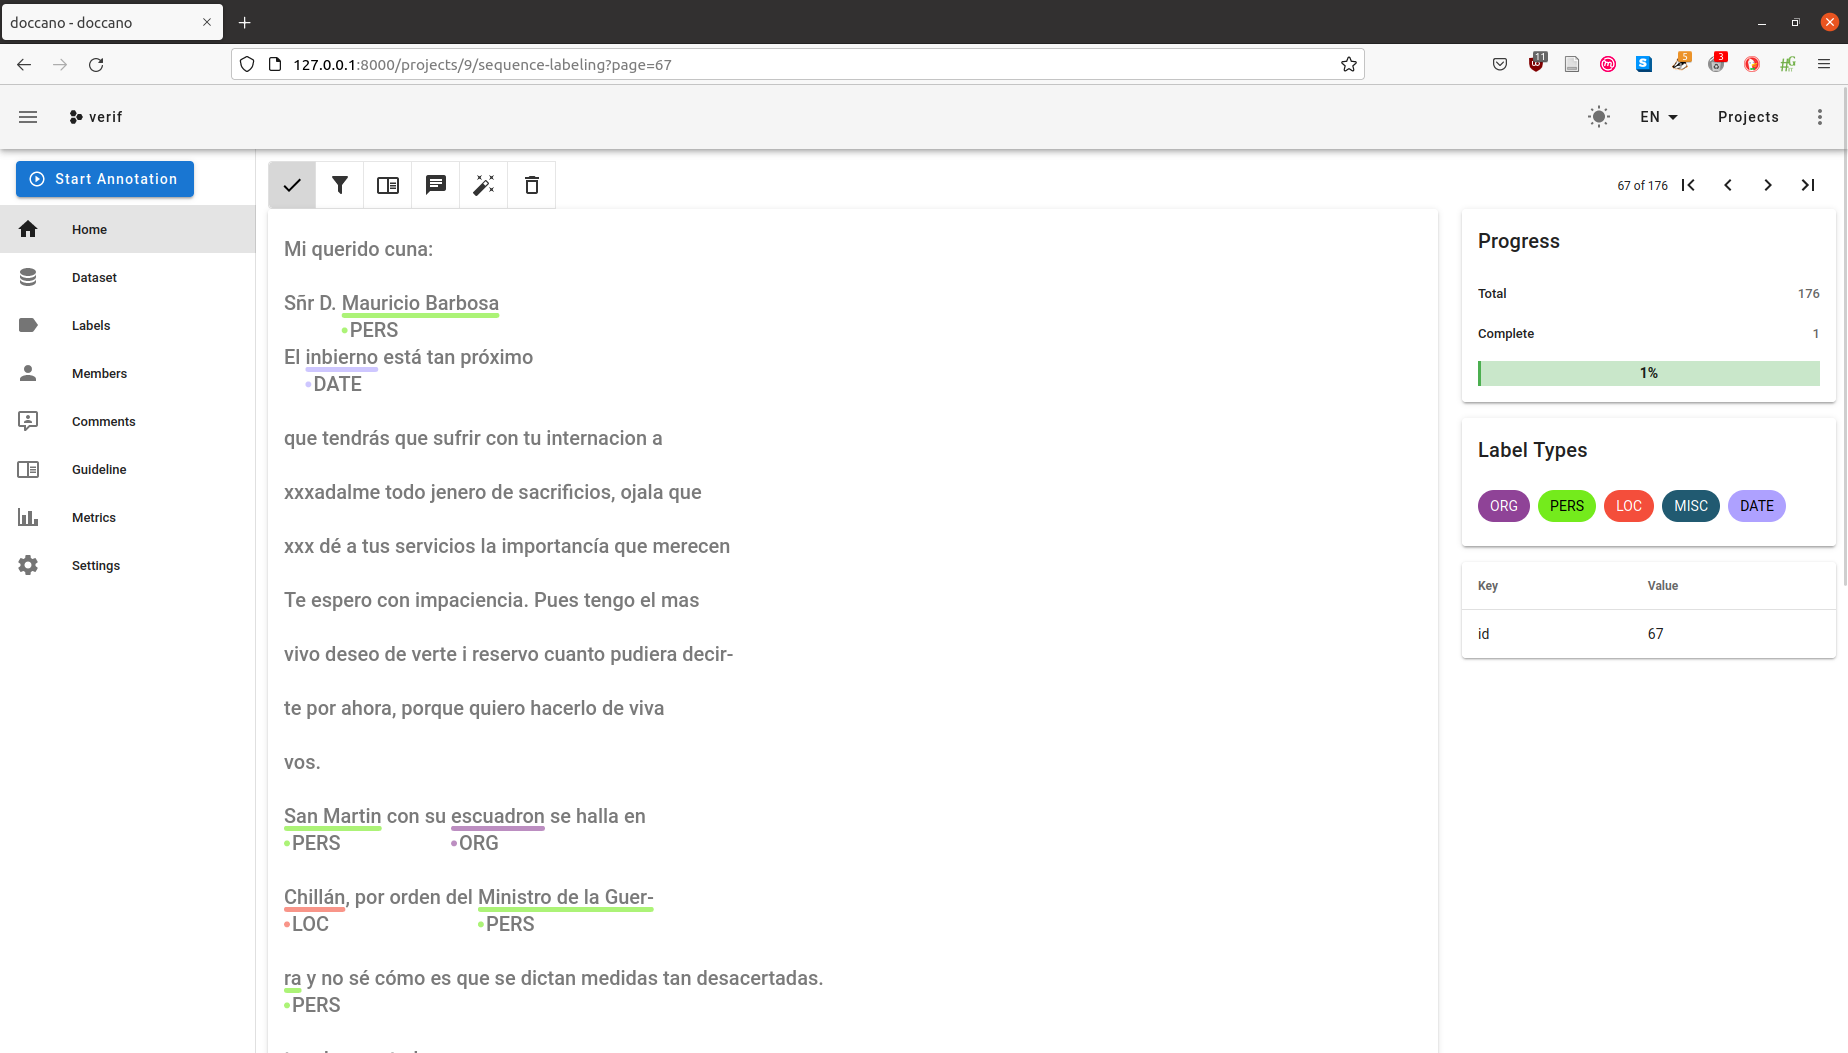
\includegraphics[width=1\textwidth]{annexes/img/doccano.png}
        \caption{Démontrastion de la plateforme Doccano}
        \label{fig:doccano}
    \end{figure}
    
    Si il est possible d'exercer une pré-annotation automatique à partir de modèle générique de NER ou d'appliquer des systèmes de règles, nous avons préféré annoter manuellement afin de s'approprier plus facilement le corpus documentaire, mais aussi les stratégies d'annotations possibles pour un corpus relativement modeste (180 documents). Pour ce faire, nous avons privilégiée la plateforme d'annotation \textit{open-source} \texttt{Doccano} pour son accessibilité et son orientation vers la librairie de \gls{tal} \gls{spacy}\footcite[Cette plateforme a été programmé avec le langage python et le \textit{framework} Django.][]{nakayamaDoccano2022}. Cet outil multifonctions d'annotation de données a été installé en local à partir du système Docker. À l'image de la figure \ref{fig:doccano}, les différentes séquences de caractères sont étiquetées de manière exclusive, c'est-à-dire à dire qu'une entité ne peut pas appartenir à une entité plus large afin d'éviter les futures confusions possibles. Cette définition a déjà été faite au sein de la conférence CoNLL 2003 où les chercheurs Erik F. Tjong Kim Sang et Fien de Meuder considéraient les entités nommées comme \enquote{non-récursive} et \enquote{\textit{non-overlapping}}\footcite{sangIntroductionCoNLL2003Shared2003}.
    
    À l'heure actuelle, \texttt{Doccano} limite l'exportation au format JSONL (pour JSON Lines), c'est-à-dire un fichier JSON dont la structuration est décomposée en plusieurs lignes. Si ce n'est pas le plus courant contrairement au format CoNLL ou autres, il permet d'obtenir une annotation simple, lisible, sans marquage et ainsi sans dissection des entités.
    
    Les schèmes IOB\footnote{I : Inside (token à l'intérieur), O: Output (token à l'extérieur), B: Beginning (token au début de l'entité). Le schème standard du format CoNLL}, BIOES\footnote{B: Beginning (début de l'entité), I : Inside (token à l'intérieur), O: Output (token à l'extérieur), E: Ending (token de fin de l'entité), S: Single element (entité consituée d'un seul token)}, BILOU\footnote{B: Beginning (token au début de l'entité), I : Inside (token à l'intérieur), L: Last (token de fin), O: Output (token à l'extérieur), U: Unit (entité constituée d'un seul token). Il est format de préférence utilisé par SpaCy.} pour les plus connus ont pour fonction d'offrir ce que l'on appelle une analyse syntaxique de surface. Le choix n'est pas anodin, car il peut avoir une incidence à la fois sur l'interopérabilité des données, mais aussi sur les performances du modèles\footcite{alshammariImpactUsingDifferent2021}. Nous avons choisi de laisser les annotations sans ce pré-marquage afin de conserver une facilité d'interagir avec les données, mais aussi d'éviter un impact négatif sur l'entraînement de notre modèle.
	
	\subsection{Produire un modèle appliquée à la reconnaissance des entités nommées}
	
	La généralisation du \textit{deep learning} a permis à l'indexation \gls{ren} des documents historiques de faire bondir les scores (\gls{f1}) de 10 à 20\%\footcite{ehrmannNamedEntityRecognition2021}. Avec les innovations entourant les architectures encodeurs-décodeurs, cette augmentation des résultats est encore plus probante sur la reconnaissance des entités nommées au sein des documents historiques au delà des problèmes qu'ils impliquent, et ce malgré un corpus pouvant être rudimentaire (50 documents annotés)\footcite{abadieBenchmarkNamedEntity2022}.
	
	\subsubsection{Entraîner un modèle NER en validation croisée}
	
	Au regard de ces observations, nous nous sommes essayé au développement d'un modèle \gls{ren} à partir du modèle pré-entraîné BETO que nous avons vu précédemment\footcite{caneteSpanishPreTrainedBERT2020}. Ce pré-entraînement permet la modification du modèle initiale afin de lui donner une tâche précise grâce au \textit{finetuning} et ainsi modifier les poids au sein de l'architecture neuronale selon nos besoins. Pour ce faire, de nombreuses librairies python permettent de mettre en œuvre ce type d'entraînement à partir de modèles pré-entraînés \textit{Transformers}. \gls{spacy} et \texttt{HuggingFace} sont sans doute à l'heure actuelle les plus populaires, car elles offrent des solutions \gls{tal} clés en main, ergonomiques et accessibles. Si elles sont par nature restrictives, elles restent suffisantes à l'ambition du projet qui ne nécessite pas une refonte neuronale totale contrairement à des projets amplement plus complexes. Nous avons privilégié l'utilisation de la librairie \gls{spacy} en raison de la galaxie de solutions \textit{softwares} qui l'entourent, le maintien d'une documentation exhaustive et extrêmement pédagogique avec la possibilité d'utiliser les modèles \textit{Transformers} grâce à la mise en place d'une \textit{pipeline} pour l'utilisation des modèles originalement disponibles au sein de la librairie \texttt{HuggingFace}\footcite{SpacytransformersUsePretrained2022}.
	
	Au préalable, il est à noter que le processus d'apprentissage de modèles \textit{Transformers} nécessite une grande puissance de calcul. Dans un premier temps, nous avons souhaité utilisé la plateforme Google Colab\footnote{\textit{Google Colab}, \url{https://colab.research.google.com/}, consulté le 04/09/2022.} mettant à disposition l'utilisation de \gls{gpu} par l'intermédiaire de leurs serveurs. Par la suite, nous avons utilisé un \gls{gpu} personnel pouvant avoir eu une incidence sur les résultats du modèles\footnote{Nvidia RTX 3080, CUDA 11.3, cuDNN}.
	
	\begin{figure}[h!]
	    \centering
	    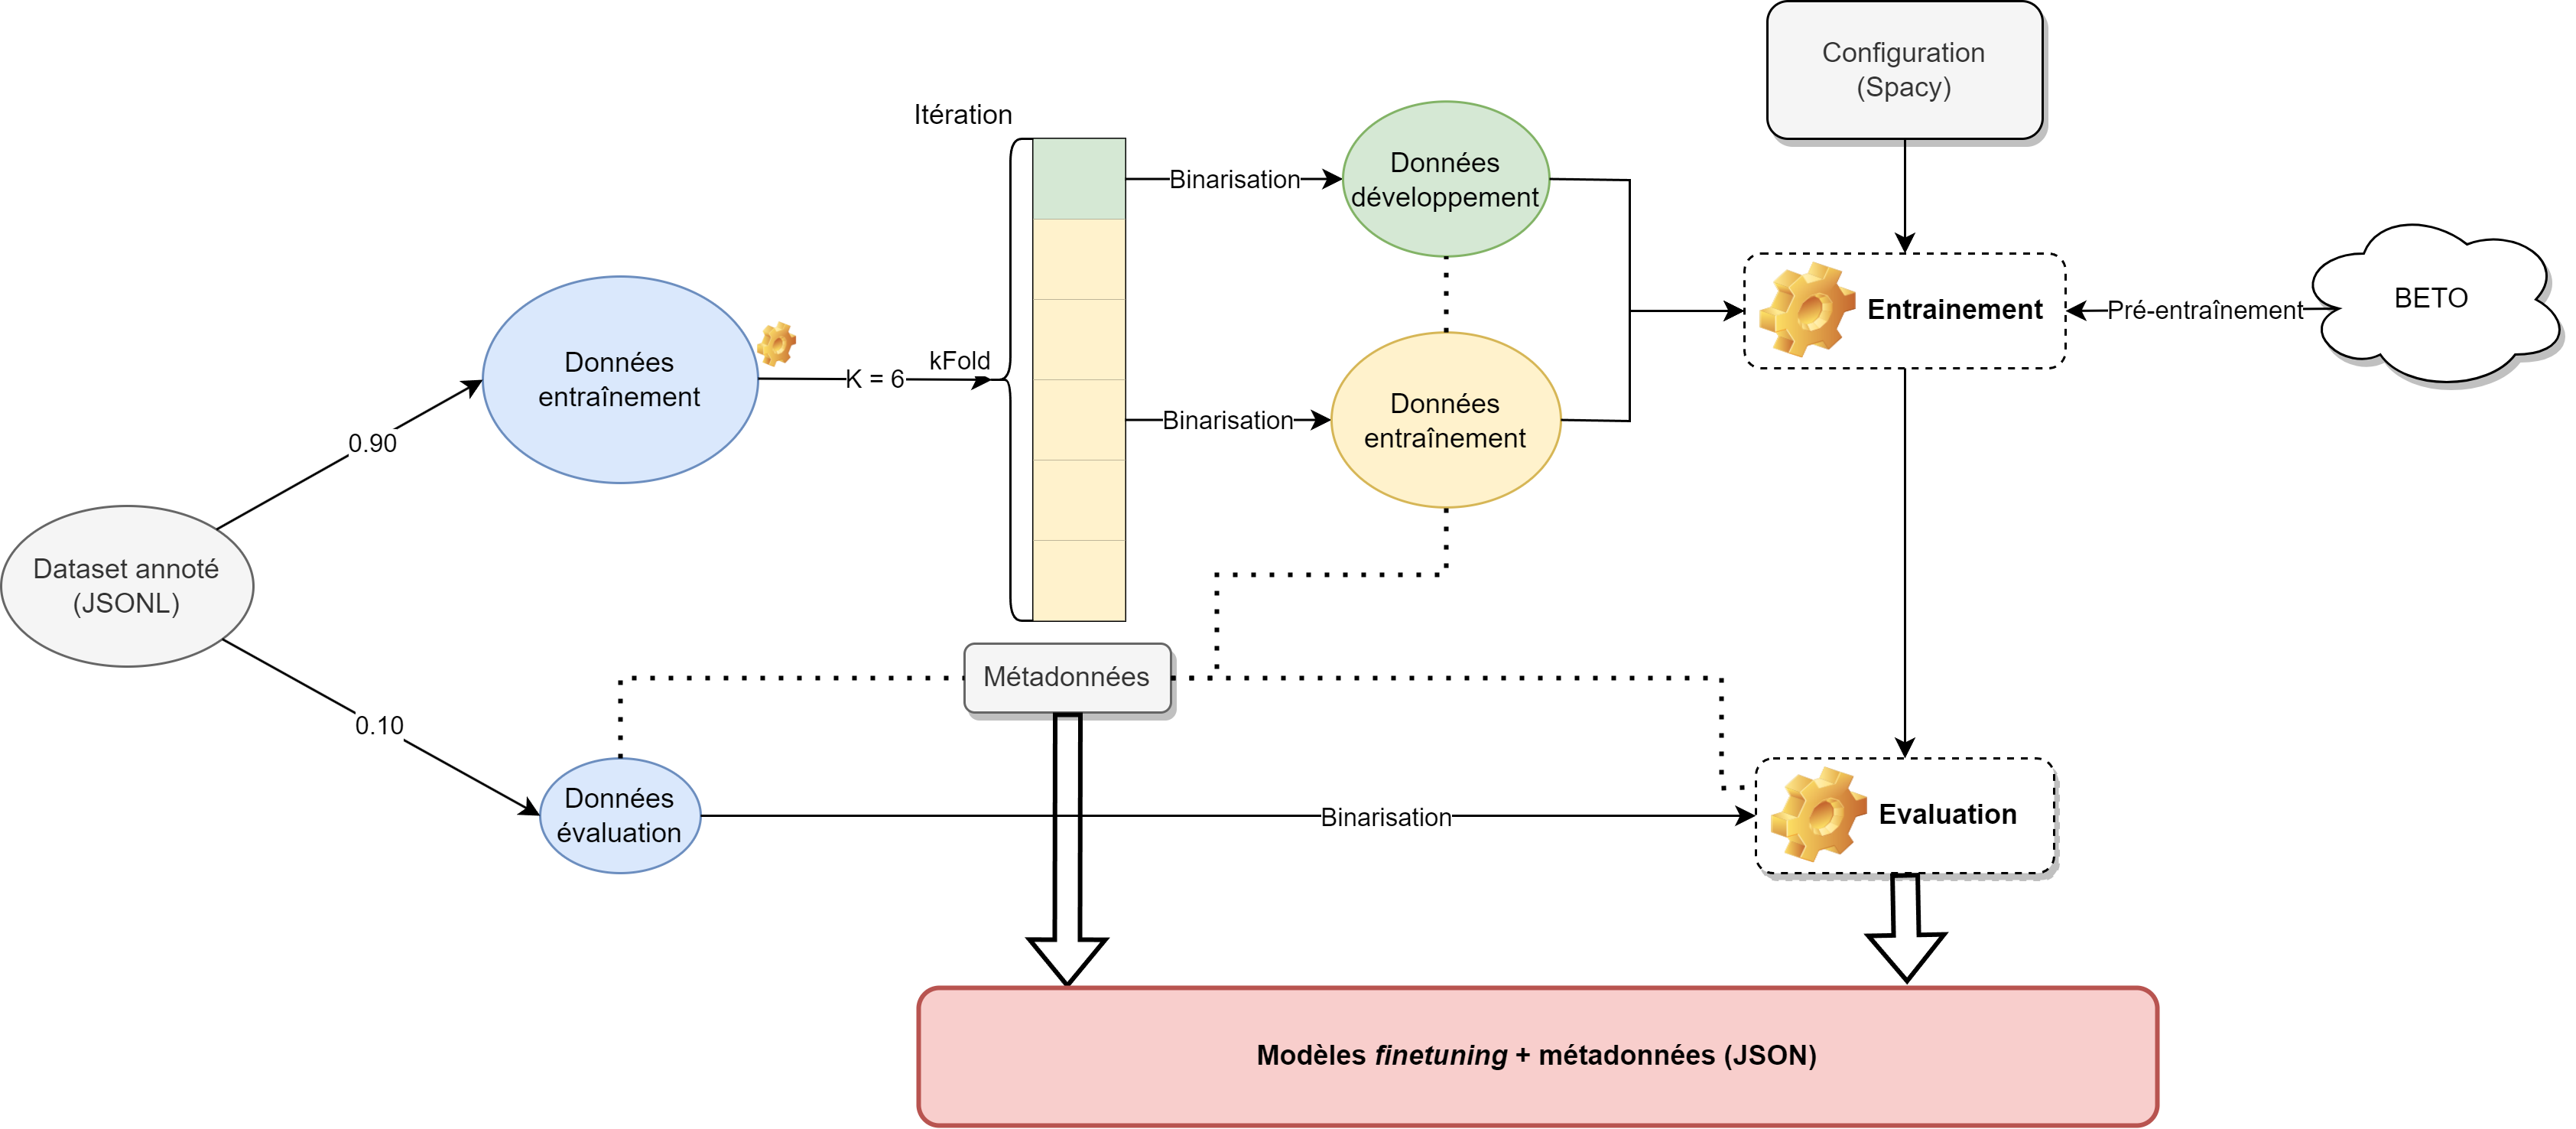
\includegraphics[width=1\textwidth]{annexes/schema/NER_training.png}
	    \caption{Schéma du processus d'entraînement d'un modèle NER en validation croisée\protect\footnotemark}
	    \label{fig:ner_cross}
	\end{figure}
	\footnotetext{\cite{humeauEntrainementAnnotationsNER2022}}
	
	Afin de mettre en oeuvre ce processus d'entraînement, nous sommes aidés de la librairie \texttt{scikit-learn} mettant à disposition un grand nombre d'outils appliqués au \textit{machine learning}\footcite{ScikitlearnScikitlearn2022}. Plus précisément, le processus s'appuie sur la séparation des données en plusieurs dépôts utilisable au cours de l'entraînement (un jeu d'entraînement et un jeu d'évaluation) afin d'offrir des jeux avec le moindre biais humain. 
	
	Dans un second temps, nous pouvons observer au sein de la figure \ref{fig:ner_cross} la présence d'une itération autour de \textit{kFold}. Cet élément correspond à la mise en place d'un procédé de validation croisée. Cette méthode K-fold, permet de tester et améliorer les performances d’un modèle prédictif en exploitant l'ensemble de notre jeu de données d'entraînement, en constituant des \textit{samples} ($\kappa$) de données partagées pour l'entraînement et sa validation. Cet technique d'apprentissage permet de maximiser le potentiel du jeu original en le prenant dans son intégralité, particulièrement quand celui-ci est restreint\footcite{perssonEffectExcludingOut2017}. Les données d'évaluation restent les mêmes tout au long du processus afin de fournir des données tests stables et ainsi fournir une évaluation fiable.
	
	Chaque itération détermine un set de données d'entraînement et de validation (qui ne pourra donc plus l'être par la suite) qui sont alors binarisées pour être exploitables par le \gls{cli} de \gls{spacy}. Le programme va effectué une première modélisation avec le modèle pré-entrainé BETO avant d'incorporer les données d'entraînement au sein de l'apprentissage. Chaque étape se conclut par un processus d'évaluation qui détermine ses performances à chaque \textit{epoch} à partir des données d'évaluation. Une fois le meilleur modèle estimé, celui-ci est évalué à partir des données tests dont les résultats sont associés à un fichier \gls{json}.
	
	\begin{figure}[h!]
	    \centering
	    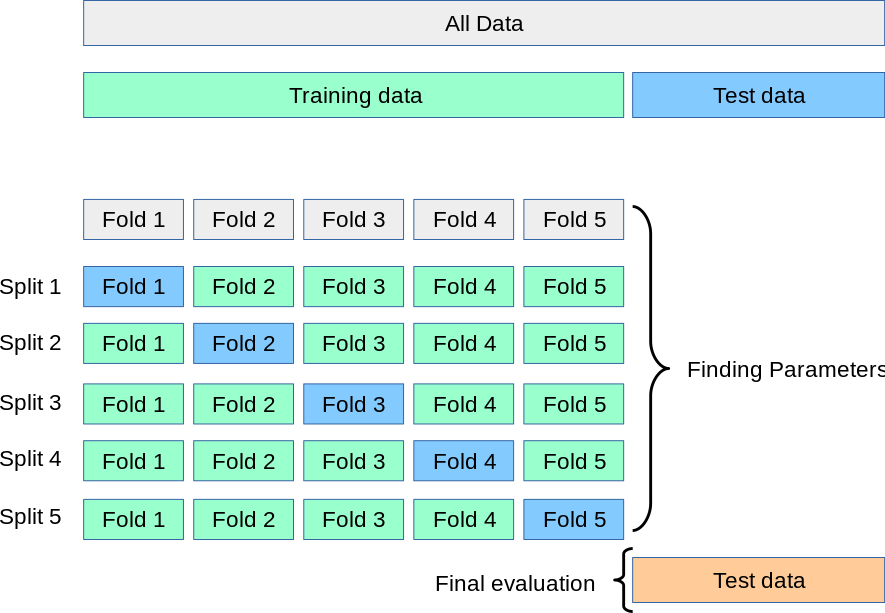
\includegraphics[width=0.5\textwidth]{annexes/schema/cross_validation.png}
	    \caption{Explication du système de validation croisée à partir de la méthode K-fold -- \copyright scikit-learn}
	    \label{fig:cross validation}
	\end{figure}
	
	\subsubsection{Interprétation des résultats et améliorations possibles}
	
	À partir de ces résultats, nous pouvons comparer les différents modèles afin de déterminer le plus performant d'entre eux\footnote{L'ensemble des données sont consultables au sein de l'annexe F.}. Cette phase d'évaluation consiste à estimer la capacité du modèle à sélectionner la bonne chaîne de caractères et d'attribuer à cette chaîne le référentiel adéquat. Pour cela, trois mesures basées sur la matrice de confusion sont considérées les plus pertinentes par la communauté scientifique: \gls{ACC}, \gls{rappel}, \gls{f1}\footcite{liSurveyDeepLearning2020}. Elles permettent d'avoir une perception globale du modèle en évaluant le taux de bonnes réponses sur les supposées entités repérées. Le score \gls{f1} décrit une valeur globale en conciliant les deux mesures\footnote{D'autres métriques plus complexes existent aussi pour l'évaluation des modèles \gls{ren} tel que la mesure SER, mais nous avons conserver les mesures proposées par \texttt{spaCy}. \cite{ehrmannNamedEntityRecognition2021}}.
	
	\begin{figure}[h!]
	    \centering
	    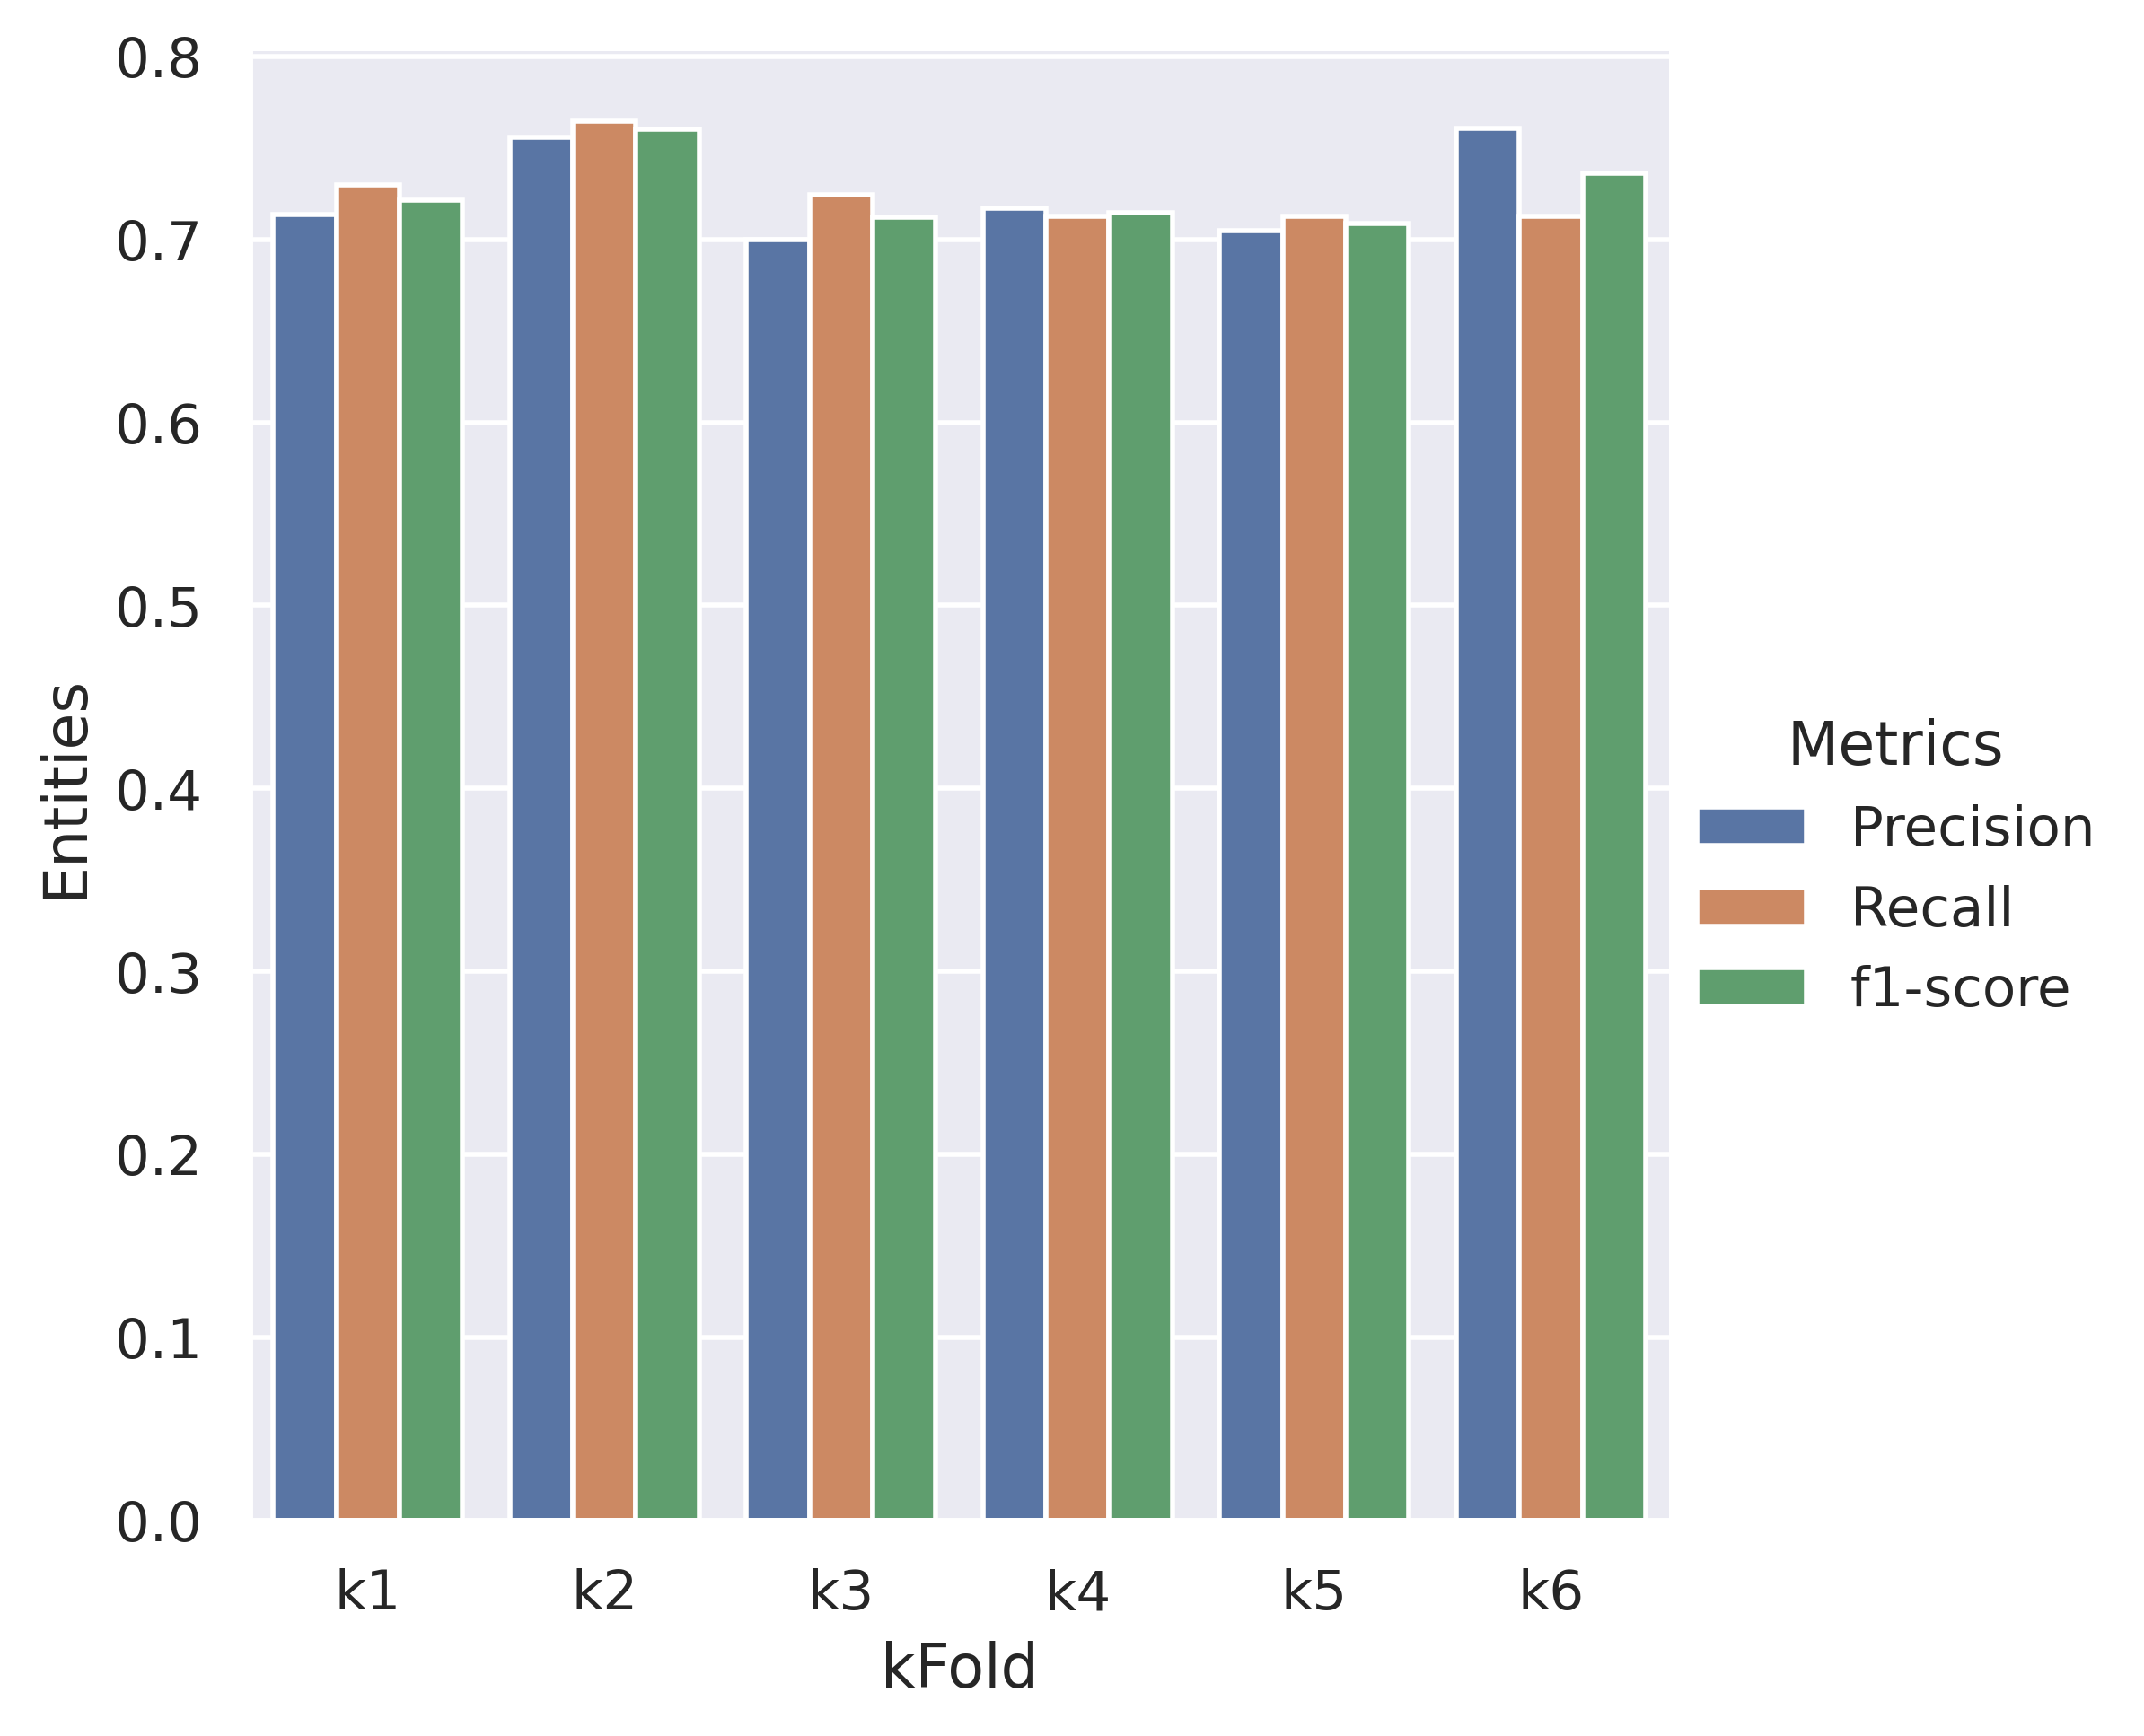
\includegraphics[width=0.4\textwidth]{annexes/graph/ent_glob.png}
	    \caption{Résultats globaux par $\kappa$ selon les trois mesures principales}
	    \label{fig:ner_global}
	\end{figure}
	
	Selon les mesures présentées, les différents modèles ont été analysés selon leurs performances comme nous pouvons l'observer au sein de la figure \ref{fig:ner_global}. Au regard des données qui ont été évaluées, deux modèles sont apparus comme les plus solides: le modèle $\kappa_2$ et le modèle $\kappa_6$. À première vue, le modèle $\kappa_2$ apparaît comme le plus satisfaisant, avec un taux de surpositivité plus faible comme le montre la valeur de \gls{rappel}.
	À la suite d'une comparaison plus approfondie entre les deux modèles sélectionnés, nous avons pu observer une lacune générale sur les entités MISC qui peut s'expliquer par la forte diversité de celle-ci. Toutefois, certaines entités semblent plus accessibles que d'autres à l'image des navires qui sont facilement identifiables\footnote{Voir l'annexe G.}. En revanche, on observe une légère supériorité du modèle $\kappa_2$ concernant les entités de type LOC, PERS et plus légèrement ORG. Sur l'ensemble, le modèle $\kappa_2$ semble produire plus de bruit dans la reconnaissance des données, ce qui s'observe avec le fort contraste entre le taux de précision et le taux de rappel. 
	
	Face à ce constat, nous avons privilégié l'emploi du modèle $\kappa_2$ qui semblent présenter des performances globales plus pertinentes dans le cadre du projet, avec une attention particulière sur les entités LOC et PERS estimés les plus indispensables à l'édition en vue de l'enrichissement des données. Sans être excellente, les performances du modèle \gls{ren} peuvent être classé comme positives si on le compare à d'autres expérimentations, plus particulièrement en raison de la faible quantité de données ajoutées\footcite[p.~105-109]{scheithauerReconnaissanceEntitesNommees2021}. De plus le réseau neuronal semble avoir rapidement assimilé l'entité DATE qui est souvent présentée de manière structurée. En revanche, on peut remarquer une forte fébrilité sur la reconnaissance de certains notamment \enquote{Usted} pouvant être associé à la fois au référentiel LOC, MISC ou ORG. De même, il semble parfois amalgamer certaines entités avec leurs prépositions.
	
	Afin de perfectionner ce modèle, deux solutions possibles ont été décrites afin de faire face aux problèmes constatés. La première est de spécifier plus en détail les entités MISC qui sont trop généralistes. L'autre axe d'amélioration est ce que l'on appelle la désambiguïsation et la relation des entités nommées (\textit{entity linking} en anglais) qui n'ont pas pu être mises en place pour l'instant faute de temps\footcite{ehrmannNamedEntityRecognition2021}. Le modèle doit être capable de reconnaître la référence d'un mot au-delà de sa polysémie. Par exemple, \enquote{Arauco} peut signifier à la fois une ville et une administration régionale. En général, cette désambiguïsation s'appuie sur l'entraînement d'un modèle à partir d'une base de connaissance extérieure en identifiant les éléments polysémiques\footcite{bunescuUsingEncyclopedicKnowledge2006}. Cette stratégie est appelée \textit{entity linking} et elle permet l'identification  du mot, par une approche vectorielle ou syntaxique, en l'alignant au près de grandes bases de connaissances accessibles \textit{via} le web sémantique\footcite{morenoApprendreRepresentationsJointes2017}.
	
	\begin{figure}[H]
         \centering
         \begin{subfigure}[b]{0.4\textwidth}
             \centering
             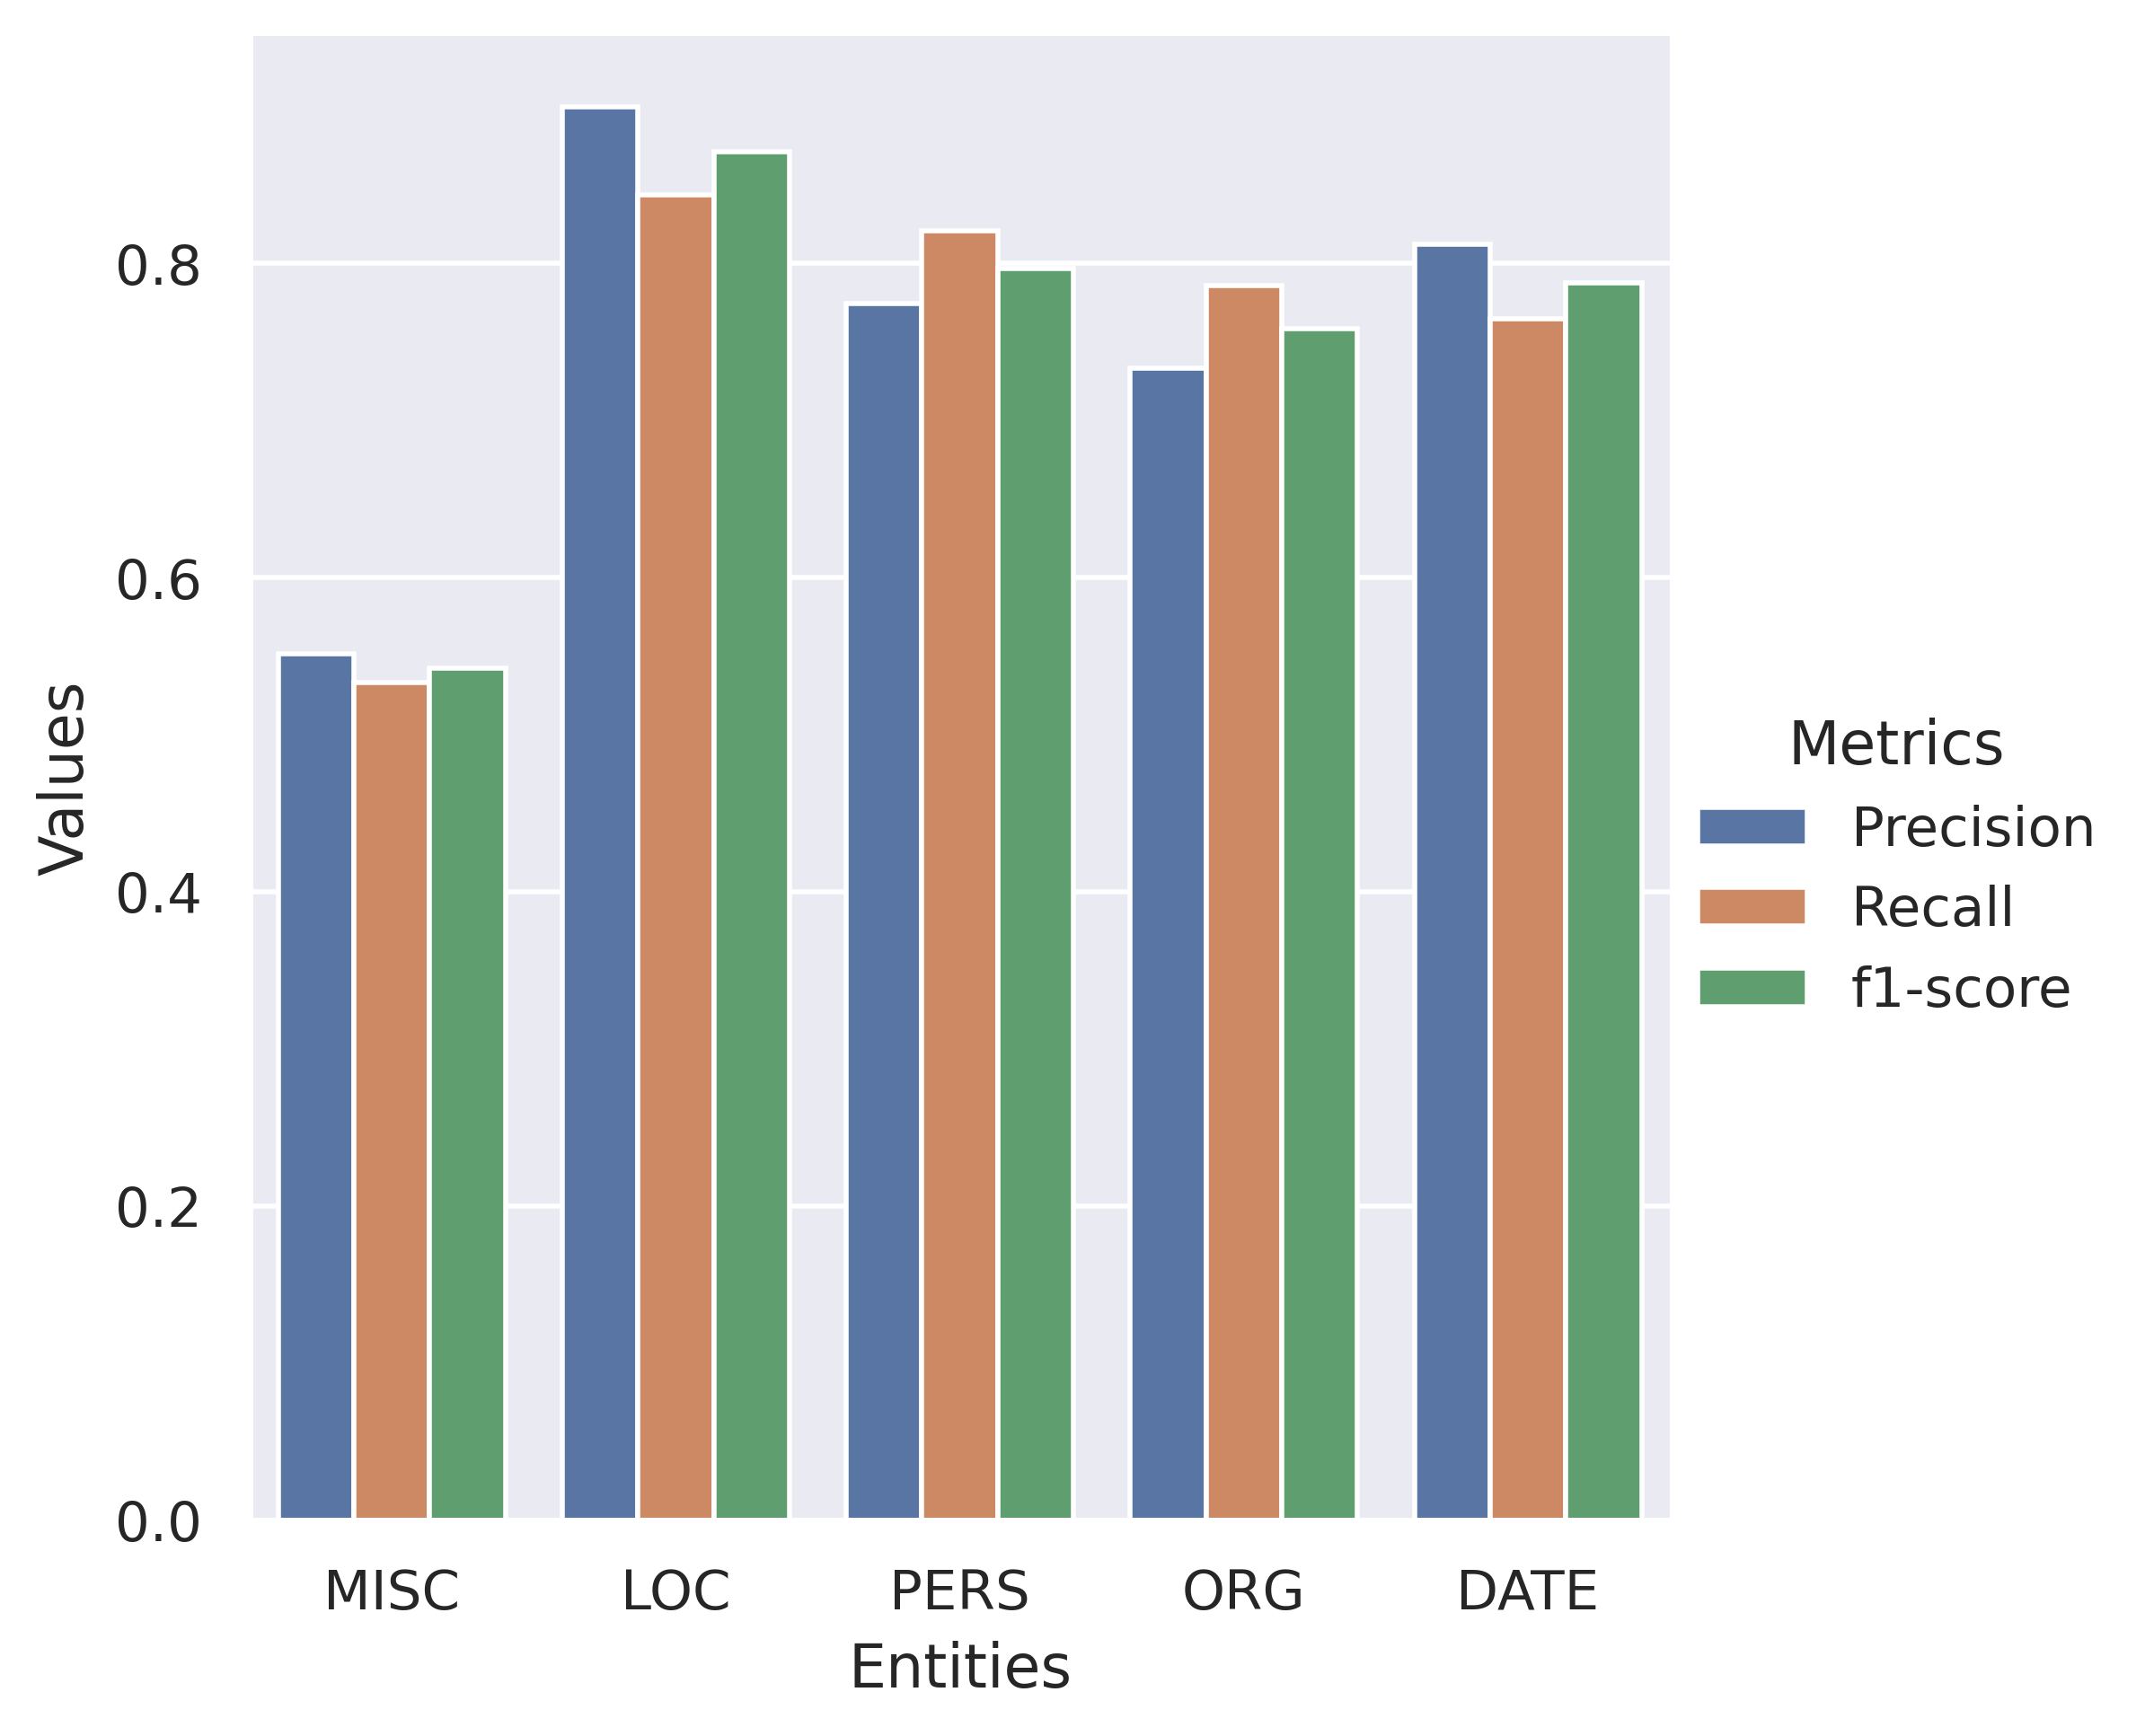
\includegraphics[width=\textwidth]{annexes/graph/k2.png}
             \caption{$\kappa_2$}
             \label{fig:k2}
         \end{subfigure}
         \hfill
         \begin{subfigure}[b]{0.4\textwidth}
             \centering
             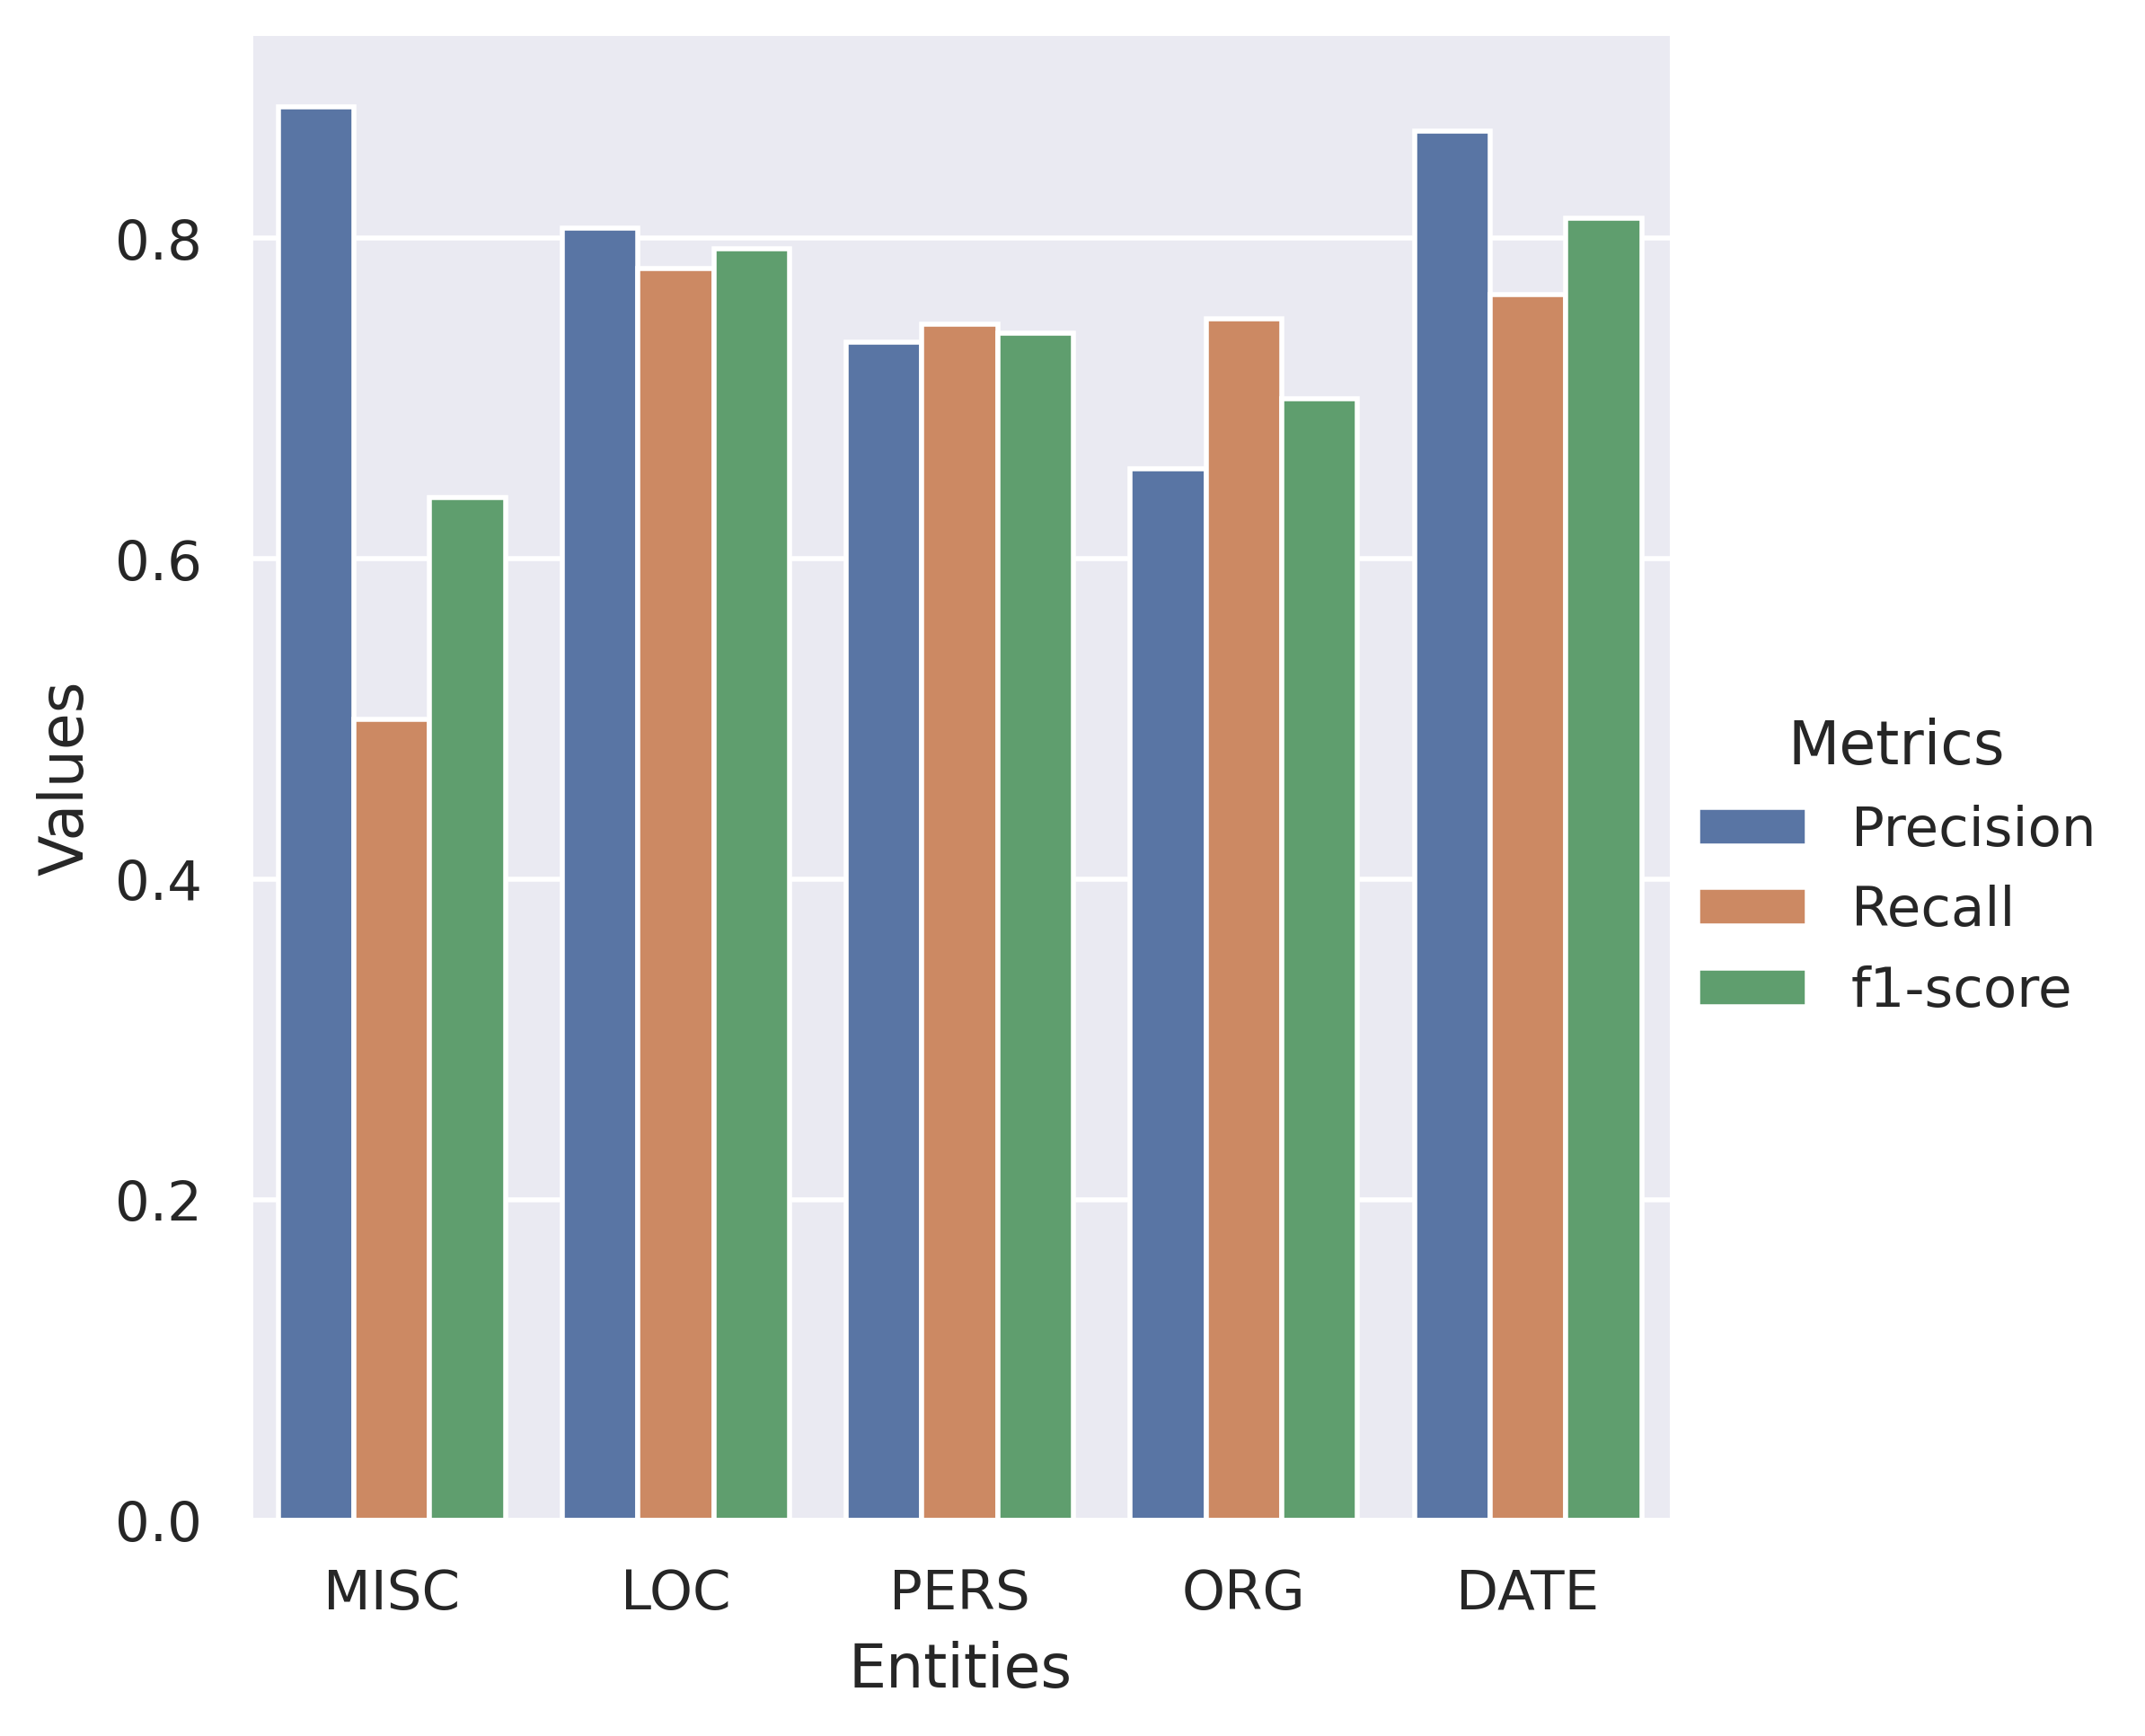
\includegraphics[width=\textwidth]{annexes/graph/k6.png}
             \caption{$\kappa_6$}
             \label{fig:k6}
         \end{subfigure}
         \caption{Résultats détaillés par entité}
        \label{fig:ner_results}
    \end{figure}
    
    \begin{table}[H]
    \centering
    \begin{tabular}{c|r|r|r|}
    \cline{2-4}
    \textbf{}                              & \multicolumn{1}{c|}{\textbf{Precision}} & \multicolumn{1}{c|}{\textbf{Rappel}} & \multicolumn{1}{c|}{\textbf{F1-score}} \\ \hline
    \multicolumn{1}{|c|}{\textbf{Général}} & 0.7556                                  & 0.7643                               & 0.7600                                 \\ \hline
    \multicolumn{1}{|c|}{\textbf{MISC}}    & 0.5517                                  & 0.5333                               & 0.5423                                 \\ \hline
    \multicolumn{1}{|c|}{\textbf{LOC}}     & 0.9000                                  & 0.8437                               & 0.8709                                 \\ \hline
    \multicolumn{1}{|c|}{\textbf{DATE}}    & 0.8125                                  & 0.7647                               & 0.7878                                 \\ \hline
    \multicolumn{1}{|c|}{\textbf{PERS}}    & 0.7746                                  & 0.8208                               & 0.7971                                 \\ \hline
    \multicolumn{1}{|c|}{\textbf{ORG}}     & 0.7333                                  & 0.7857                               & 0.7586                                 \\ \hline
    \end{tabular}
    \caption{Évaluation des performances du modèle $\kappa_2$}
    \label{tab:k2_benchmark}
    \end{table}
	
	
	\section{Indexer, enrichir et exploiter les données}
	
	La reconnaissance des entités nommées offre une double opportunité. Elle permet dans un premier temps d'indexer l'ensemble des entités et ainsi faciliter l'accès à cette donnée pour l'utilisateur ou l'utilisatrice. L'autre aspect est la capacité de renforcer les mécanismes d'enrichissement au cours du processus éditorial. Cet enrichissement est en général un exercice conséquent et pour autant nécessaire dans la constitution d'un apparat critique\footcite{campsOuVaPhilologie2018}.
	 
	 Dans cette perspective nous allons observer la mise en place d'un processus d'indexation et d'enrichissement automatique grâce à l'aide de l'\textit{open data} et les problématiques que ce procédé impose.
	
	\subsection{Indexer les entités nommées au sein d'une édition numérique TEI}
	
	La première difficulté qui a été rencontré dans l'application d'un schéma d'indexation a été simplement d'appliquer la reconnaissance au sein d'un fichier structuré et de conserver cette structuration, dans notre cas \gls{xml} et de l'encodage \gls{tei}. Au retour des campagnes d'annotations ESTER, Solenn Le Pevedic et Denis Maurel approuvent la capacité de l'encodage à manipuler les entités nommées en permettant une normalisation des éléments descriptifs\footcite{lepevedicRetourAnnotationsEntites2016a}. Au sein de cet article, les auteurs vont émettre de premières recommandations sur le balisage de ces entités en fonction de leur référentiel, et les attributs adéquats, en reprenant le guide Quaero.
	
	\begin{figure}[h!]
	    \centering
	    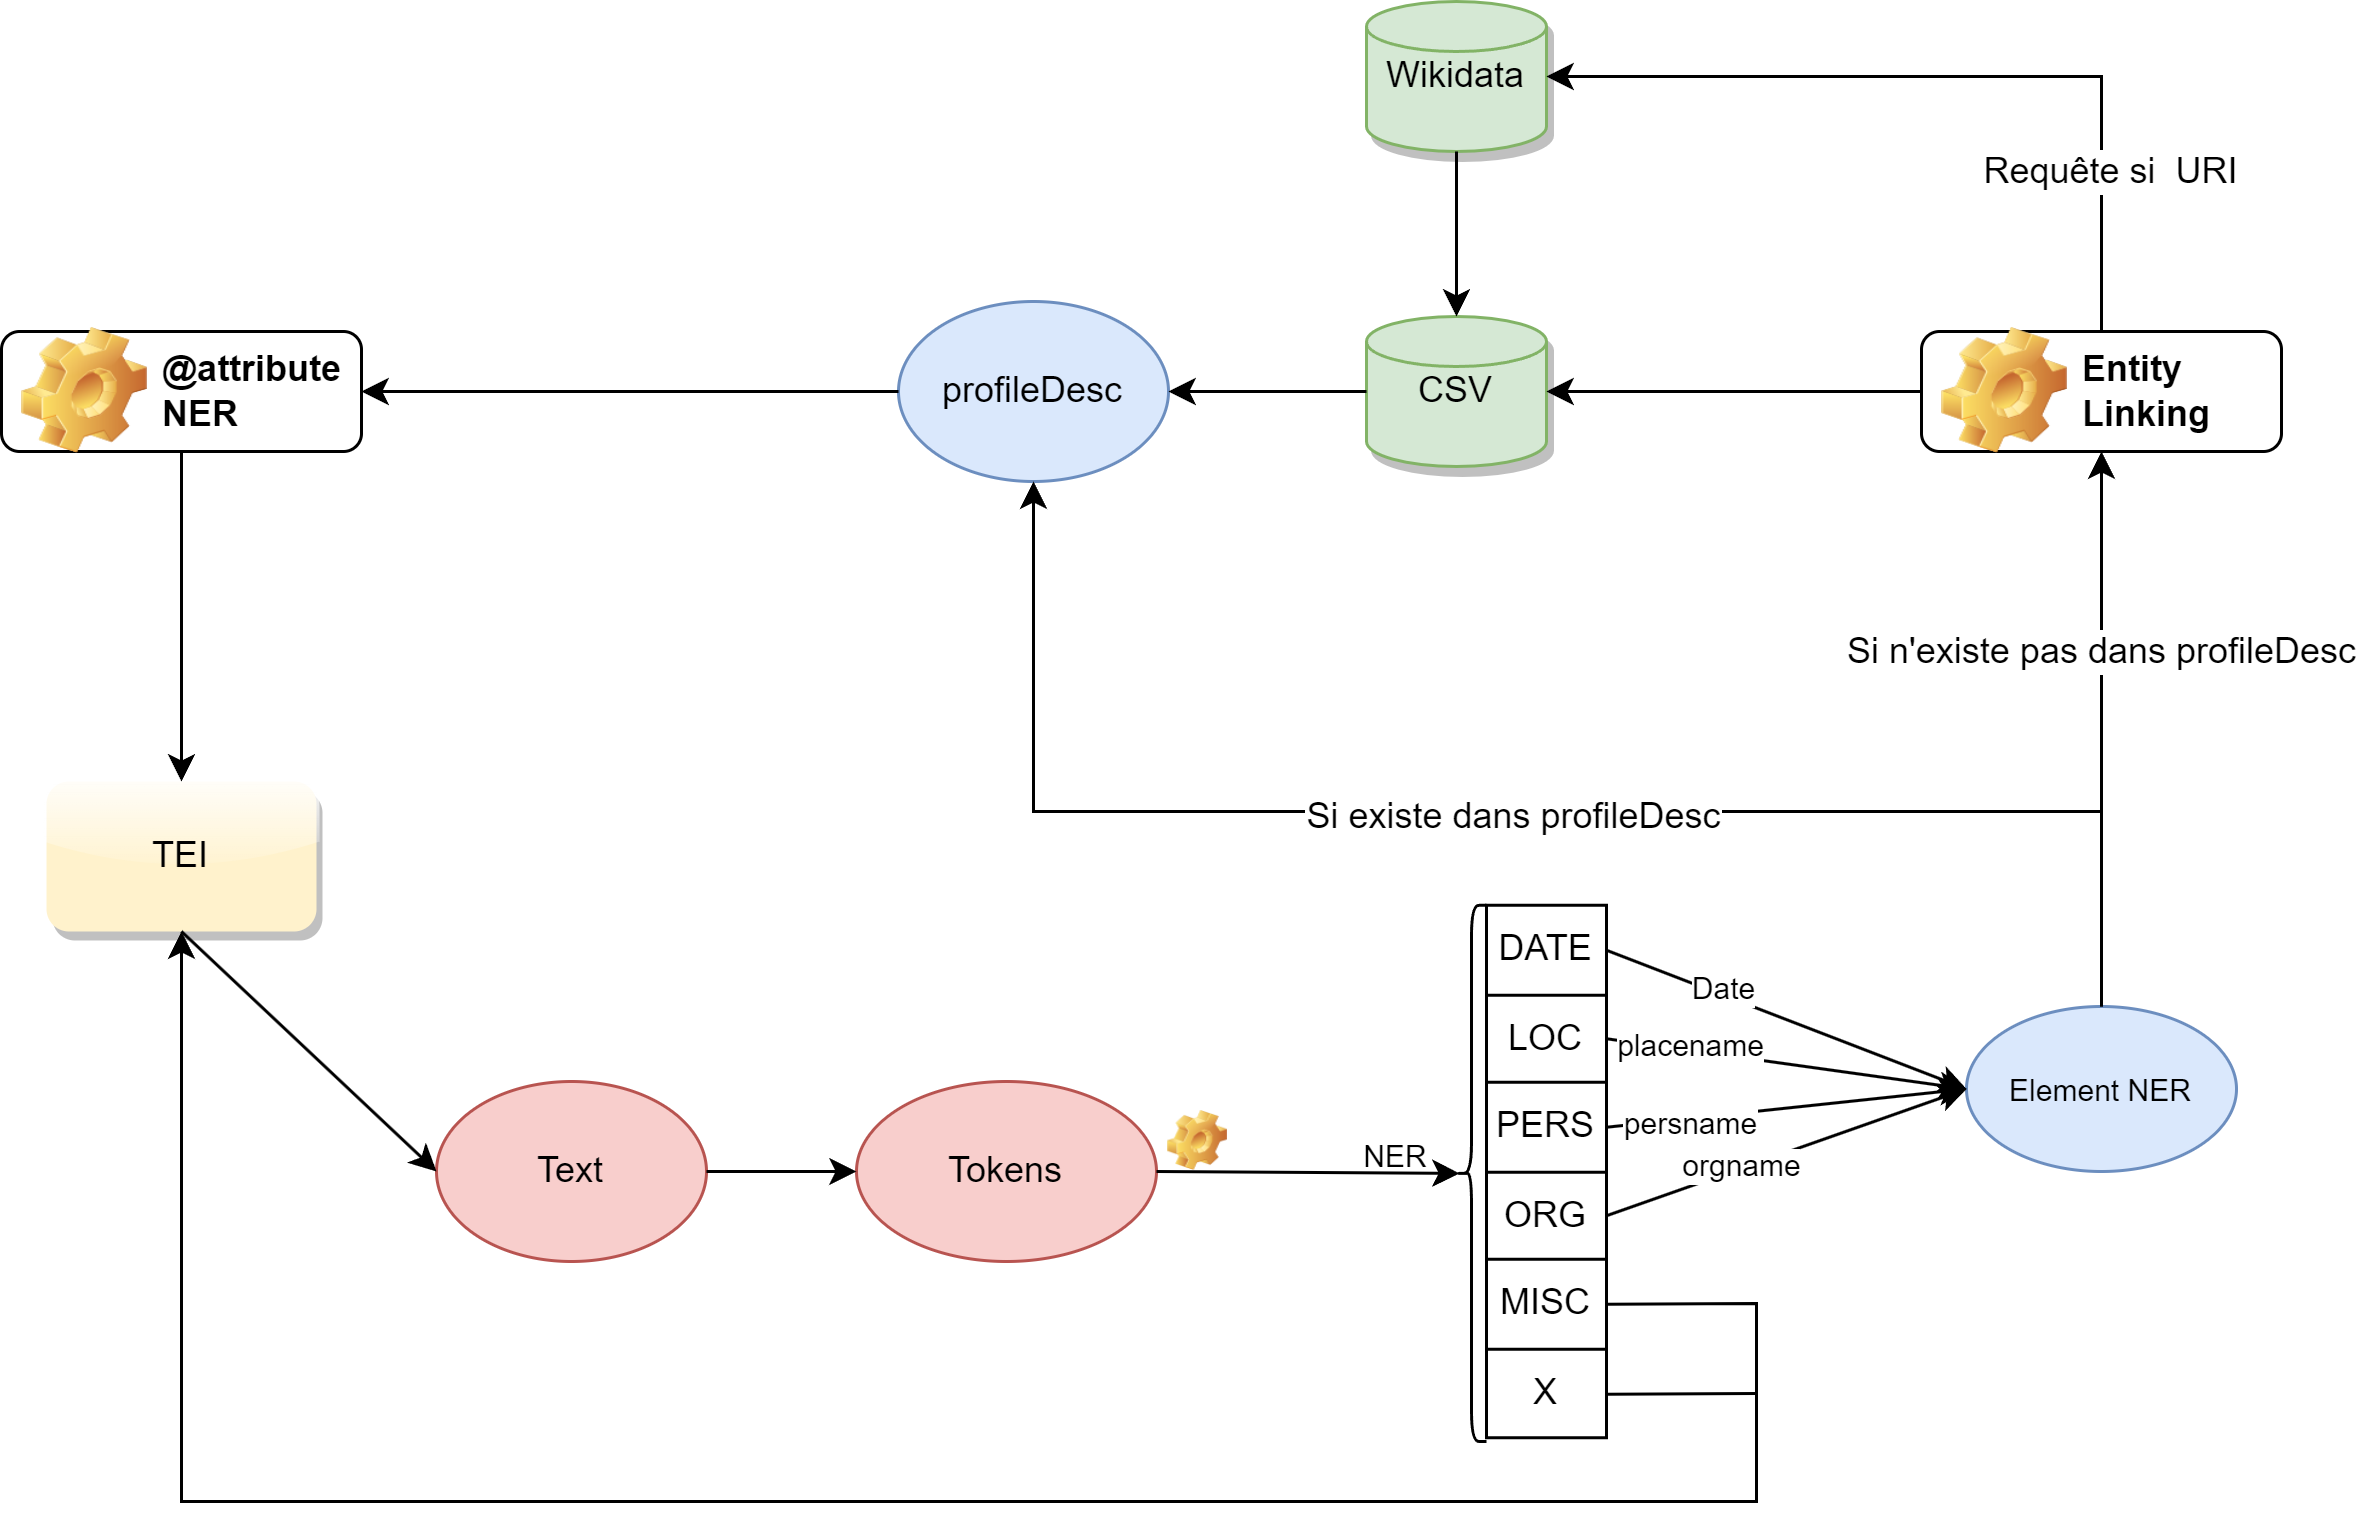
\includegraphics[width=0.8\textwidth]{annexes/schema/ner_index.png}
	    \caption{Système d'indexation des entités nommées au sein d'un fichier XML-TEI}
	    \label{fig:ner_index}
	\end{figure}
	
	Pour manipuler nos fichiers XML-TEI déjà existants, nous nous sommes appuyés sur la librairie \texttt{StandoffConverter} développée récemment par David Lassner\footcite{lassnerStandoffconverter2021}. L'utilisation de son \gls{API} permet le balisage des entités détectées par le modèle développé\footcite[Le script est visible au chemin suivant : TEI\_tranformation/src/enrichment/nlp.py \textit{in}][]{humeauTeiTransformation2022}. Pour ce faire, la classe StandoffConverter va analyser l'ensemble du \balise{text}, le tokeniser et repérer son référentiel au sein des catégories définies par le modèle \gls{ren}. Cette librairie a permis de faciliter ce travail d'extraction et les problèmes sous-jacents en limitant l'impact de la structuration \gls{xml} en permettant de convertir certains éléments sous la syntaxe \gls{regex}, par exemple : \balise{lb} pour \textbackslash n.
	
	Pour chaque entité, nous avons remis les recommandations de balisage émises par S. Le Pevedic et D. Maurel en les simplifiant afin de permettre l'automatisation de l'indexation\footcite{lepevedicRetourAnnotationsEntites2016a}. Ainsi, l'entité DATE est balisée sous l'élément \balise{date}, LOC est balisée sous l'élément \balise{placename}, PERS est balisée sous l'élément \balise{persname} et ORG est balisé sous l'élément \balise{orgname}. À l'inverse, les tokens MISC ou sans labélisation ne sont pas référencés dans le fichier XML-TEI final.\newpar
	
	Les entités balisées sont ensuite analysées par la librairie \texttt{spaCy Fishing} afin de déterminer les possibles ambiguïtés et pouvoir les aligner au sein du web sémantique. Cette librairie a été développée par Lucas Terriel, inspiré par les travaux de Patrice Lopez sur la désambiguïsation des entités nommées et les fonctions d'\textit{entity linking}\footcite{terrielSpaCyFishing2022}. Elle est une fonctionnalité rattachable aux fonctions sommaires de \gls{spacy}, faisant la liaison entre la détection d'entités nommées et l'identification au sein d'une base de connaissances, ici \textit{Wikidata}. Si le score de l'évaluation de cette requête est supérieur à 0.8, l'\gls{uri} de l'entité (ex: Q4233309 pour Cornelio Saavedra Rodríguez) est alors conservée et enregistrée au sein de la base de données \gls{csv}, sinon un identifiant est généré si l'entité n'est pas déjà référencée au sein de la base de données.
	
	Cette chaîne d'extraction d'informations a dans le même temps été appliquée au sein du projet NER4Archives\footcite{clavaudNER4ArchivesNamedEntity2022}. Néanmoins, dans notre cas les résultats donnés par cette pratique de \textit{fishing} ont démontrés de nombreuses lacunes. Les premiers essais ont montré une réelle difficulté à déterminer et aligner la bonne entité avec un haut niveau de certitude. La gestion des abréviations n'ayant pu être pour l'instant incorporée au sein du processus de transformation, l'alignement avec la base de données \texttt{wikidata} ne peut se faire correctement.
	
	\subsection{Le web de données : SPARQL et Wikidata}
	
	L'identifiant des entités nommées permet l'accès d'un point de référence à la fois au sein de la base de données \gls{csv}, mais aussi à l'intérieur de notre encodage \gls{tei}. Au sein des éléments, cet identifiant est indiqué à l'intérieur d'un attribut \attribut{ref} le reliant directement à son élément parent présent au sein des index définis par la \gls{tei}. Pour le cas des entités LOC, celles-ci sont enregistrées au sein du \balise{settingDesc}, alors que les entités ORG et PERS sont quant à elles recensées au sein du \balise{particDesc}. Ce référencement permet de décrire plus en détail les différents éléments indexés.
	
	Comme le rappelle Simon Hengchen et al., l'effervescence du web de données a eu un réel impact auprès des secteurs culturels en donnant des points d'accès à des bases de données permettant d'enrichir considérablement leurs propres collections\footcite{hengchenExtractionEntitesNommees2015}. Une méta-étude recense justement que la recherche et l'exploration de données sont les principaux facteurs dans le choix de mettre en place ces bases de données liées\footcite{davisLinkedDataCultural2021}. La \gls{ren} sert de point d'accroche avec les données présentes au sein de web de données (\textit{linking data}). Cette notion est apparue dans les années 1990 sous l'égide de Tim Berner-Lee qui la définit comme un espace d'échange de documents permettant d'accéder à leurs contenus et effectuer des raisonnements\footcite{berners-leeSemanticWeb2001}. Les contenus sont communément appelés des ressources qui doivent être organisées de manière structurée afin d'être intelligible, souvent à partir de la syntaxe \gls{rdf}.  La relation sémantique entre les ressources est possible sous la forme de \enquote{triplet} : Sujet (ressource principale) -- Prédicat (relation) -- Objet (ressource secondaire). La représentation \gls{rdf} va s'appuyer sur un ensemble de classes (Sujets) et de propriétés intrinsèques permettant d'être reliée entre elles.
	
	\begin{figure}[H]
	\centering
    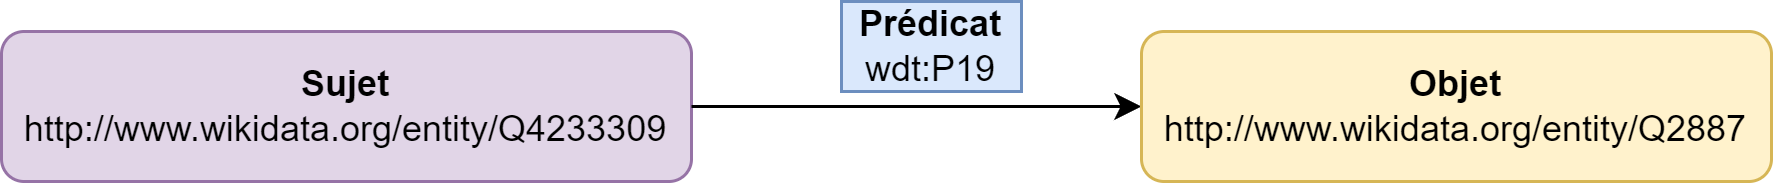
\includegraphics[width=0.7\textwidth]{annexes/schema/triplet.png}
    \begin{minted}[fontsize=\footnotesize]{xml}
          <?xml version="1.0"?>
          <rdf:RDF xmlns:wdt="http://www.wikidata.org/prop/direct/" xmlns:schema="http://schema.org/">
            <rdf:Description rdf:about="http://www.wikidata.org/entity/Q4233309">
               <wdt:P373>Cornelio Saavedra Rodriguez</wdt:P373>
               <wdt:P19 rdf:resource="http://www.wikidata.org/entity/Q2887"/>
            </rdf:Description>
            <rdf:Description rdf:about="http://www.wikidata.org/entity/Q2887">
               <schema:name xml:lang="en">Santiago</schema:name>
               <schema:description xml:lang="en">capital city of Chile</schema:description>
            </rdf:Description>
          </rdf:RDF>
        \end{minted}
      \caption{Structuration d'un triplet au sein d'un fichier XML-RDF}
      \label{fig:triplet}
    \end{figure}
	
	En partant de notre recherche prélimaines à partir de \texttt{spaCy Fishing}\footcite{terrielSpaCyFishing2022}, nous avons donc pu récupérer l'\gls{uri} de cette ressource au sein de la Base de données orientée graphe \textit{Wikidata}\footnote{Une base de données orientée graphe (et plus exactement orienté objet) reprend la théorie des graphes en mathématique, en permettant de représenter et stocker et de mettre en relation les données à travers des graphes.}. Au sein du web de données, cette base de donndonnéesée est sans doute la plus populaire et la plus active puisqu'elle  provient directement de l'activité Wikipedia\footnote{En 2012, on recense plus de 15 millions d'entités, dont plus de 34 millions de déclarations, et plus de 80 millions d'étiquettes et de descriptions dans plus de 350 langues. \cite{erxlebenIntroducingWikidataLinked2014}}. 
	À l'aide de l'\gls{uri}, il a été possible d'émettre une requête, différente selon la nature de l'entité, au sein de \textit{Wikidata} grâce au langage \texttt{SPARQL}. “SPARQL Protocol and RDF Query Language” est un langage standard pour interroger les données de graphes représentés par des triplets \gls{rdf}. Comme nous pouvons le voir au sein de l'application développée\footcite[Voir le fichier TEI\_tranformation/src/enrichment/sparql.py .][]{humeauTeiTransformation2022}, il a été possible de récupérer les informations suivantes :
	\begin{itemize}
	    \item Label
	    \item Fate de naissance et de mort
	    \item Identifiant numérique (VIAF ou Geoname)
	    \item Coordonnées géographiques
	    \item Adresse (région, pays)
	    \item Nationalité
	    \item Description
	\end{itemize}
	
	Une fois les informations récupérées (dans leur intégralité ou non), celles-ci sont corrigées et traitées afin de pouvoir être alignées et enregistrées au sein de la base de données \gls{csv}. Enfin les données sont alors modélisées parmi l'élément \gls{tei} correspondant au sein du \balise{particDesc} pour les personnes identifiées et \balise{settingDesc} pour les entités géographiques (voir les exemples au sein de l'annexe H).
	
	\subsection{Limites et solutions aux web de données}
	
	Les premiers essais d'enrichissement automatique avec l'utilisation de requêtes \texttt{SPARQL} ont pu démontrer le bon fonctionnement global du processus. Néanmoins, il a été relevé une certaine légèreté des données acquises, notamment pour les catégories descriptives. \textit{Wikidata} reste une base de données généraliste qui n'a pas pour vocation ni à prétendre à l'exhaustivité, ni à la valeur d'une autorité scientifique.
	
	Il est à rappeler que \textit{Wikidata} n'est pas l'unique base de données s'appuyant sur le web sémantique et disponible au grand public. D'autres bases de données graphes s'appuient sur le même modèle à l'image de \textit{DBpedia} développé par l'Université de Leipzig et l'Université libre de Berlin à partir de 2007\footnote{\textit{DBpedia}, url: \url{https://www.dbpedia.org/}, consulté le 09/09/2022.}; \textit{esDBpedia} mis en place en 2011 et maintenu par l'Ontology Engineering Group (OEG), ETSI Informáticos et l'Universidad Politécnica de Madrid\footnote{\textit{esDBpedia}, url:\url{https://es.dbpedia.org/}, consulté le 09/09/2022.}. Ces bases de données graphes conçues sur le modèle des \gls{lod} s'appuie sur l'extraction des données structurées depuis l'encyclopédie participative Wikipedia. 
	
	Une autre solution a été imaginée selon la conversion d'une édition web du \textit{Diccionario Geográfico de la República de Chile} en fichier \gls{json}\footcite{solanoasta-buruagaDiccionarioGeograficoRepublica1899}. Ce dictionnaire géographique publié à la fin du XIX\textsuperscript{e} siècle recense plus de 5197 lieux géographiques du Chili et à ses frontières. Cette transformation \gls{json} a pour but de retrouver les données de l'époque et ainsi de pouvoir s'aligner les variations orthographiques historiques ou les nominations historiques.\newpar
	Enfin, la Biblioteca del Congreso Nacional de Chile (Bibliothèque du Congrès national du Chili, en français) qui, à l'image de nombreuses institutions culturelles, a mis en place sa propre base de données reprenant les principes du \gls{lod}. Ce projet \texttt{datos.bnc.cl} dont le développement a débuté en 2011, est l'une des premières bases de données a initié ce type de projet en Amérique latine avec pour objectif initial de mettre à disposition du public le travail législatif\footcite{cifuentes-silvaArchitectureAdoptionProcess2011}. Dans le même temps, un point d'accès API (un \textit{endpoint)} a été mis en place afin d'offrir la possibilité de requêter la base de données graphe avec le langage \texttt{SPARQL}\footnote{Le site est consultable à l'adresse suivante : \url{http://datos.bcn.cl/es/}, consulté le 10/09/2022.}. Deux types de données pourraient permettre d'étayer le projet d'enrichissement : les bases de données biographiques recensant un grand nombre de personnalités de la vie politique et plus secondairement, militaires; et les données géographiques (à l'heure actuelle, l'ontologie est en cours de mise à jour). Dans un autre registre, il est à considérer que l'État chilien a lui aussi créé une infrastructure numérique nationale recensant et donnant accès à un ensemble de \textit{dumps} (dépôt de données) dans un objectif de transparence au sein de la gouvernance des données. Ils sont issus des données officielles enregistrés par le gouvernement et l'administration nationale du Chili\footnote{Le site de dépôt est consultable à cette adresse url: \url{https://datos.gob.cl/}}.
	
	Si dans ce dernier cas il fut difficile de trouver des données pertinentes dans le cadre de notre projet, l'essor de la pratique du \gls{lod} au sein de la vie scientifique, mais aussi civique chilienne est symptomatique des nombreux enjeux qui ont entouré la mise en place du projet autour des archives de l'Araucania. Les chercheurs Felipe Gonzalez-Zapata et Richard Heeks ont explicité le rôle du \textit{Open government data} pour continuer de rompre avec un passé trouble en redonnant de la valeur à l'information\footcite{gonzalez-zapataMultipleMeaningsOpen2015}.
	
	%conclusion
	\chapter*{Conclusion}
\chaptermark{Conclusion}
\addcontentsline{toc}{chapter}{Conclusion}

Ce mémoire et ce stage ont été l'occasion de mettre en évidence ou de confirmer certaines appréciations sur le développement d'une chaîne de traitement automatique pour la production d'édition numérique native. De la production d'un modèle \gls{htr} à l'analyse, l'annotation et l'enrichissement des éditions restent un processus complexe qui doit s'inscrire dans une dynamique globale. Le projet sur les archives autour de l' \enquote{Occupation de l'Araucania} est particulièrement révélateur de ces attentes.

Si la scientificité des données repose l'apport quantitatif, mais aussi critique que le chercheur y apporte. Il en reste que l'automatisation du processus de traitement représente des avantages considérables pour les institutions patrimoniales et scientifiques, sans pour autant prétendre à une exhaustivité. Le travail de l'ingénierie se tâche de concevoir et d'ajuster du mieux possible les différents programmes afin de procéder au traitement le plus complet possible, mais qui se confrontent bien souvent à de nombreuses problématiques techniques et intellectuelles.\newpar

En premier lieu, la mise en place d'un tel projet nécessite de mettre en œuvre un travail conséquent de préparation de données sur lequel va se centrer l'ensemble du programme. Il faut donc pouvoir saisir l'essence des documents qui constituent notre réservoir et notre objet d'études. L'ensemble de cette \textit{pipeline} se nourrit de ses données afin de pouvoir alimenter, poursuivre et améliorer le rendu de celles-ci. L'apprentissage automatique est ainsi devenu un axe majeur de notre réflexion et de notre pratique. Son introduction doit être considérée non pas comme finalité, et ce malgré la plus-value esthétique que ces techniques représentent, mais comme un moyen avec ces faiblesses, ces biais et ses réussites.

Ces méthodes d’apprentissages ont permises de numériser un grand nombre de nouvelles données sous l'encodage \gls{tei} et ce à partir de données océrisées. Les technologies \gls{htr} ont été des outils efficaces pour la numérisation native des documents historiques et ainsi servir leur pérennité. Pour cela, la mise en place d'un prototype d'une transformation vers le format pivot a été nécessaire.

Toutefois, il en est ressorti de nombreuses difficultés quant à leurs traitements postérieurs, ce qui induit le besoin de nouvelles réflexions sur les données présentant des défis variations orthographiques historiques. La faible homogénéité des données produites a amenée à utiliser et mettre en place un modèle de reconnaissance des entités nommées afin de procéder à l'indexation des entités majeures et laisser l'opportunité d'explorer plus en profondeur les documents ou de l'enrichir. De même, l'automatisation de la segmentation reste une étape difficile à automatiser. Cette chaîne de traitement ne peut se passer de l'intervention directe de l'humain afin d'en contrôler la qualité et la cohérence.

En observant le filigrane de ce projet, nous avons pu de même observer l'enjeu que représente l'ouverture des données, de la cohérence de leurs partages et la mise en place de plateformes communes. Ces initiatives permettent une véritable mutualisation des efforts permettant de soutenir des projets de moindre envergure qui peuvent s'appuyer sur des programmes plus vastes. En outre, ces données ouvertes interrogent sur notre rapport à la construction et l'appropriation de la science \enquote{en adoptant une posture humble et ouverte devant nos sources, sans appropriation indue et sans dissimuler la possibilité de l’erreur — mieux, en fournissant à la communauté non seulement les résultats de nos recherches, mais aussi la manière dont ils ont été produits et peuvent être reproduits\footcite{campsOuVaPhilologie2018}}. Ces données doivent pour s'émanciper de l'autorité productrice afin de dévoiler de nouvelles perceptions au travers de nouveaux regards éthiques, méthodologiques ou socio-politiques.\newpar

Le projet de ce stage a conclu au développement d'un mille-feuille dont chaque étape ne prend sens que collectivement si qui nécessite un travail en amont. Le numérique ne peut s'éloigner ou s'émanciper des méthodes humanistes, devant au contraire s'accommoder afin de faire face aux enjeux du \textit{big data} ou des nouvelles méthodes numériques. Pour Dominique Boullier, les sciences sociales ne peuvent pas être le fruit d'une numérisation de leurs méthodes, de leurs données et de leur objet d’étude, mais en apporter une valeur ajoutée\footcite{boullierSociologieNumerique2016}. Cette volonté d'enrichir s'appuie sur cette volonté d'utiliser ces nouvelles méthodes afin d'inciter ces nouvelles perceptions épistémologiques, mais aussi des nouveaux enjeux autour de la valorisation numérique. Víctor Gayol et Jairo Antonio Melo Flórez appellent, justement, les instituions a développer ces projets, notamment autour de l'histoire digital afin de sortir des expériences individuelles allant au détriment d'une véritable cohérence\footcite{gayolPresentePerspectivasHumanidades2017}.

Ces humanités numériques  restent en plein essor et entourés d'espoirs sur la compréhension d'une histoire complexe ou la mémoire est encore douloureuse. Du Chili au Mexique, ce champs des humanités s'organise et se construit progressivement afin de faciliter la circulation des savoir-faire et des données à l'image du réseau RED\footnote{Red de Humanidades Digitales, url: \url{http://humanidadesdigitales.net/}, consulté le 30/08/2022}. La multiplication des efforts conjoints et de mise en parallèle avec des projets vont permettre révéler et encourager les archives autour de l'\enquote{Occupation de l'Araucanie} afin d'encourager l'émergence d'une nouvelle historiographie sur ces évènements\footcite{canalestapiaHistoriografiaMapucheBalances2015}.


	
	%glossaire si glossaire
	\glsaddall
    \printglossary[type=\acronymtype, nonumberlist]
    \printglossary[nonumberlist]
	%\printglossaries
	
	%les annexes
	\appendix

\addcontentsline{toc}{part}{Annexes}

\part*{Annexes}

\chapter{Le fonds Araucania}
\begin{figure}
	    \centering
    	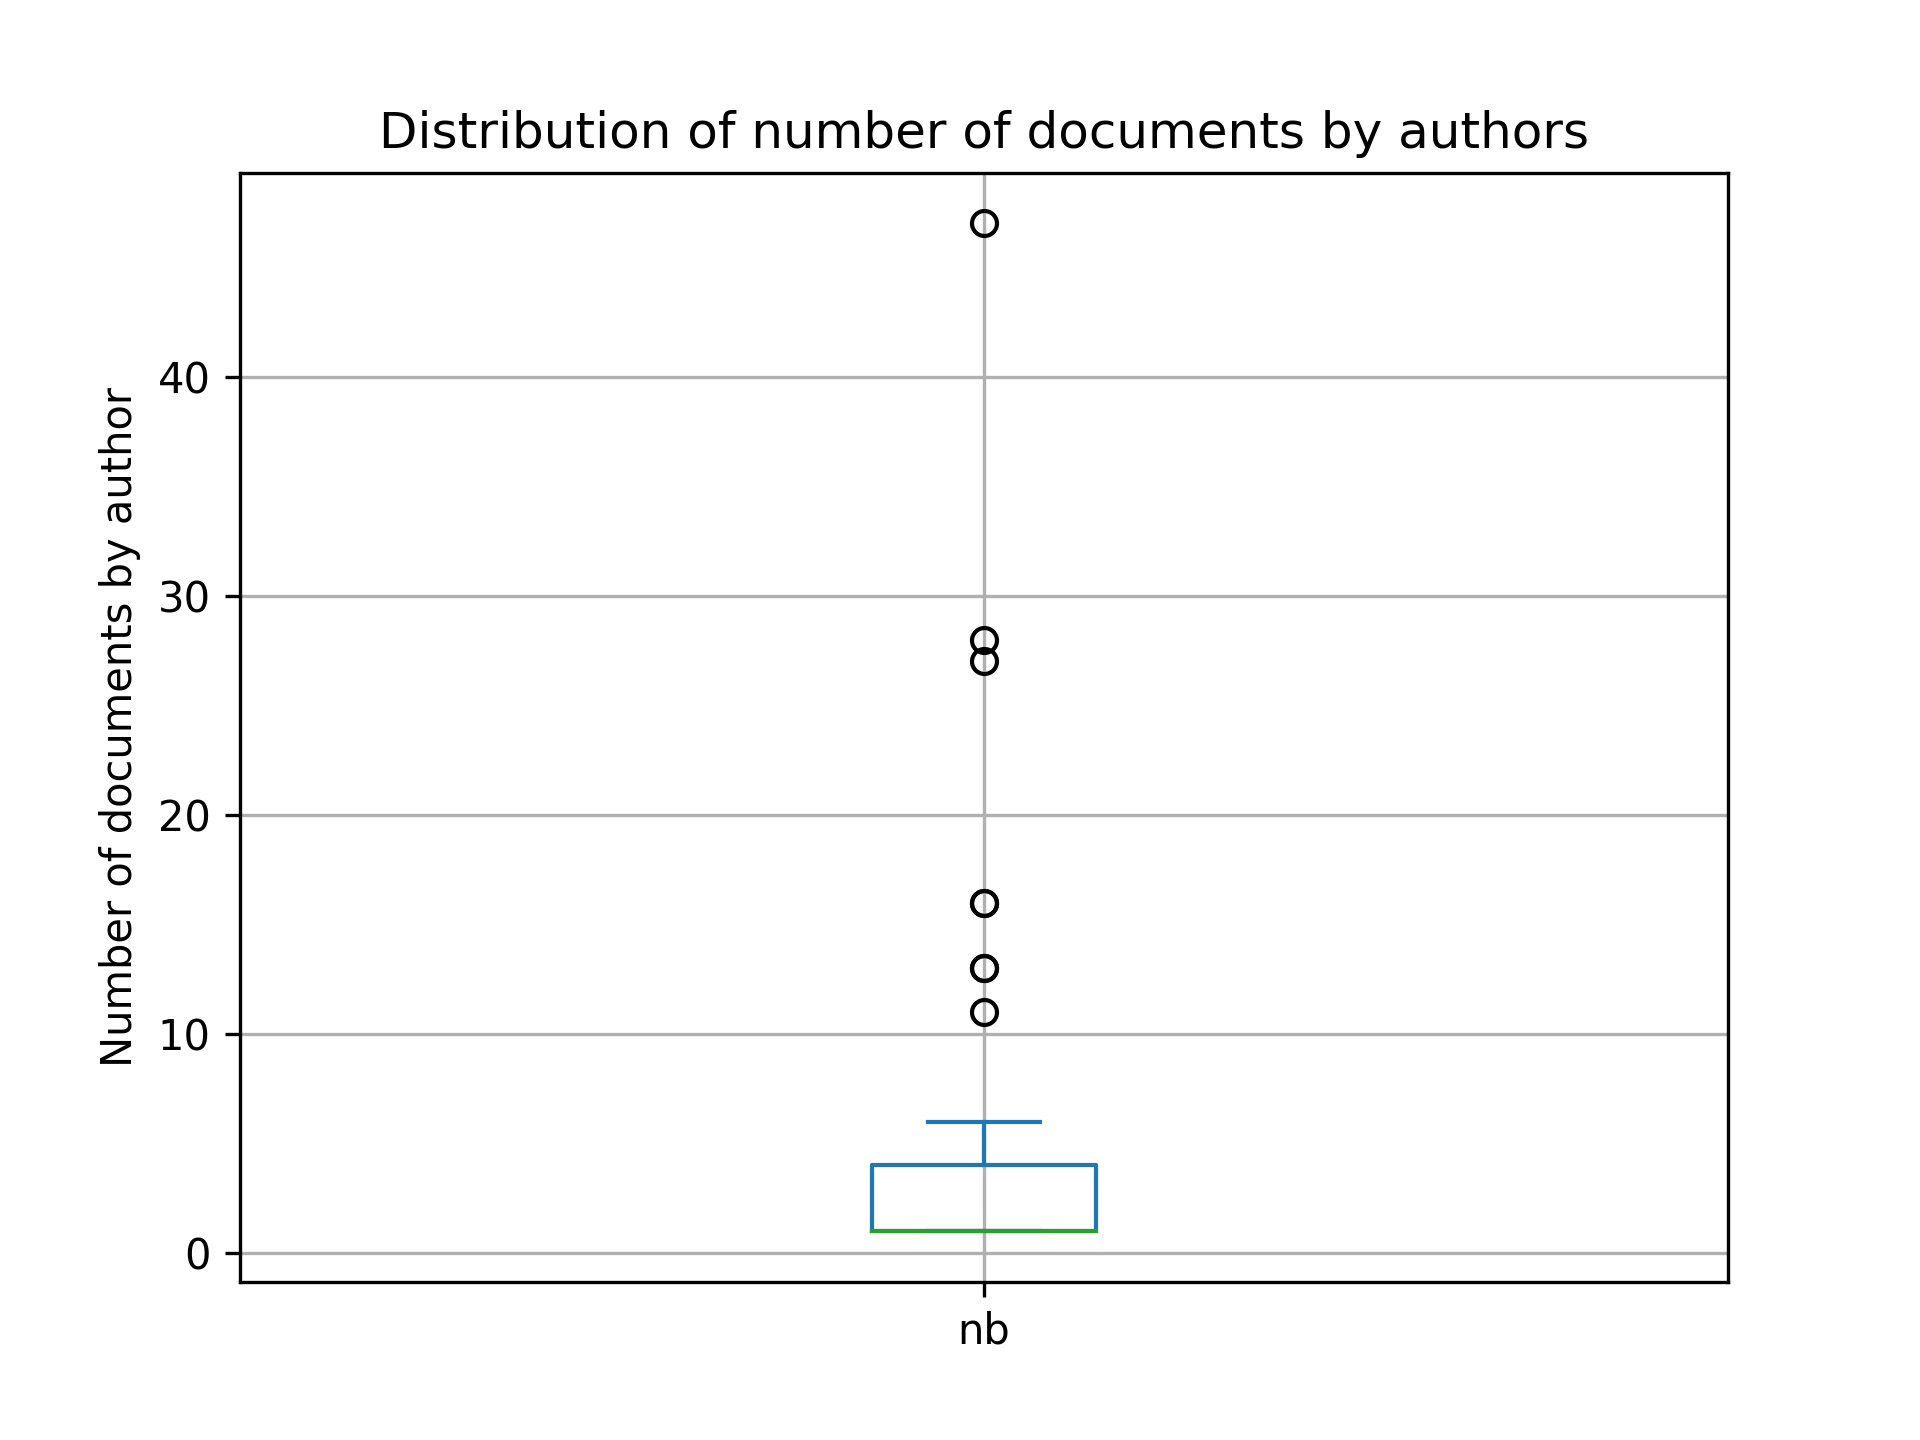
\includegraphics[width = 1\textwidth]{annexes/graph/author_distribution.png}
    	\caption{Distribution du nombres de documents par auteurs}
    	\label{fig:author_distribution}
    	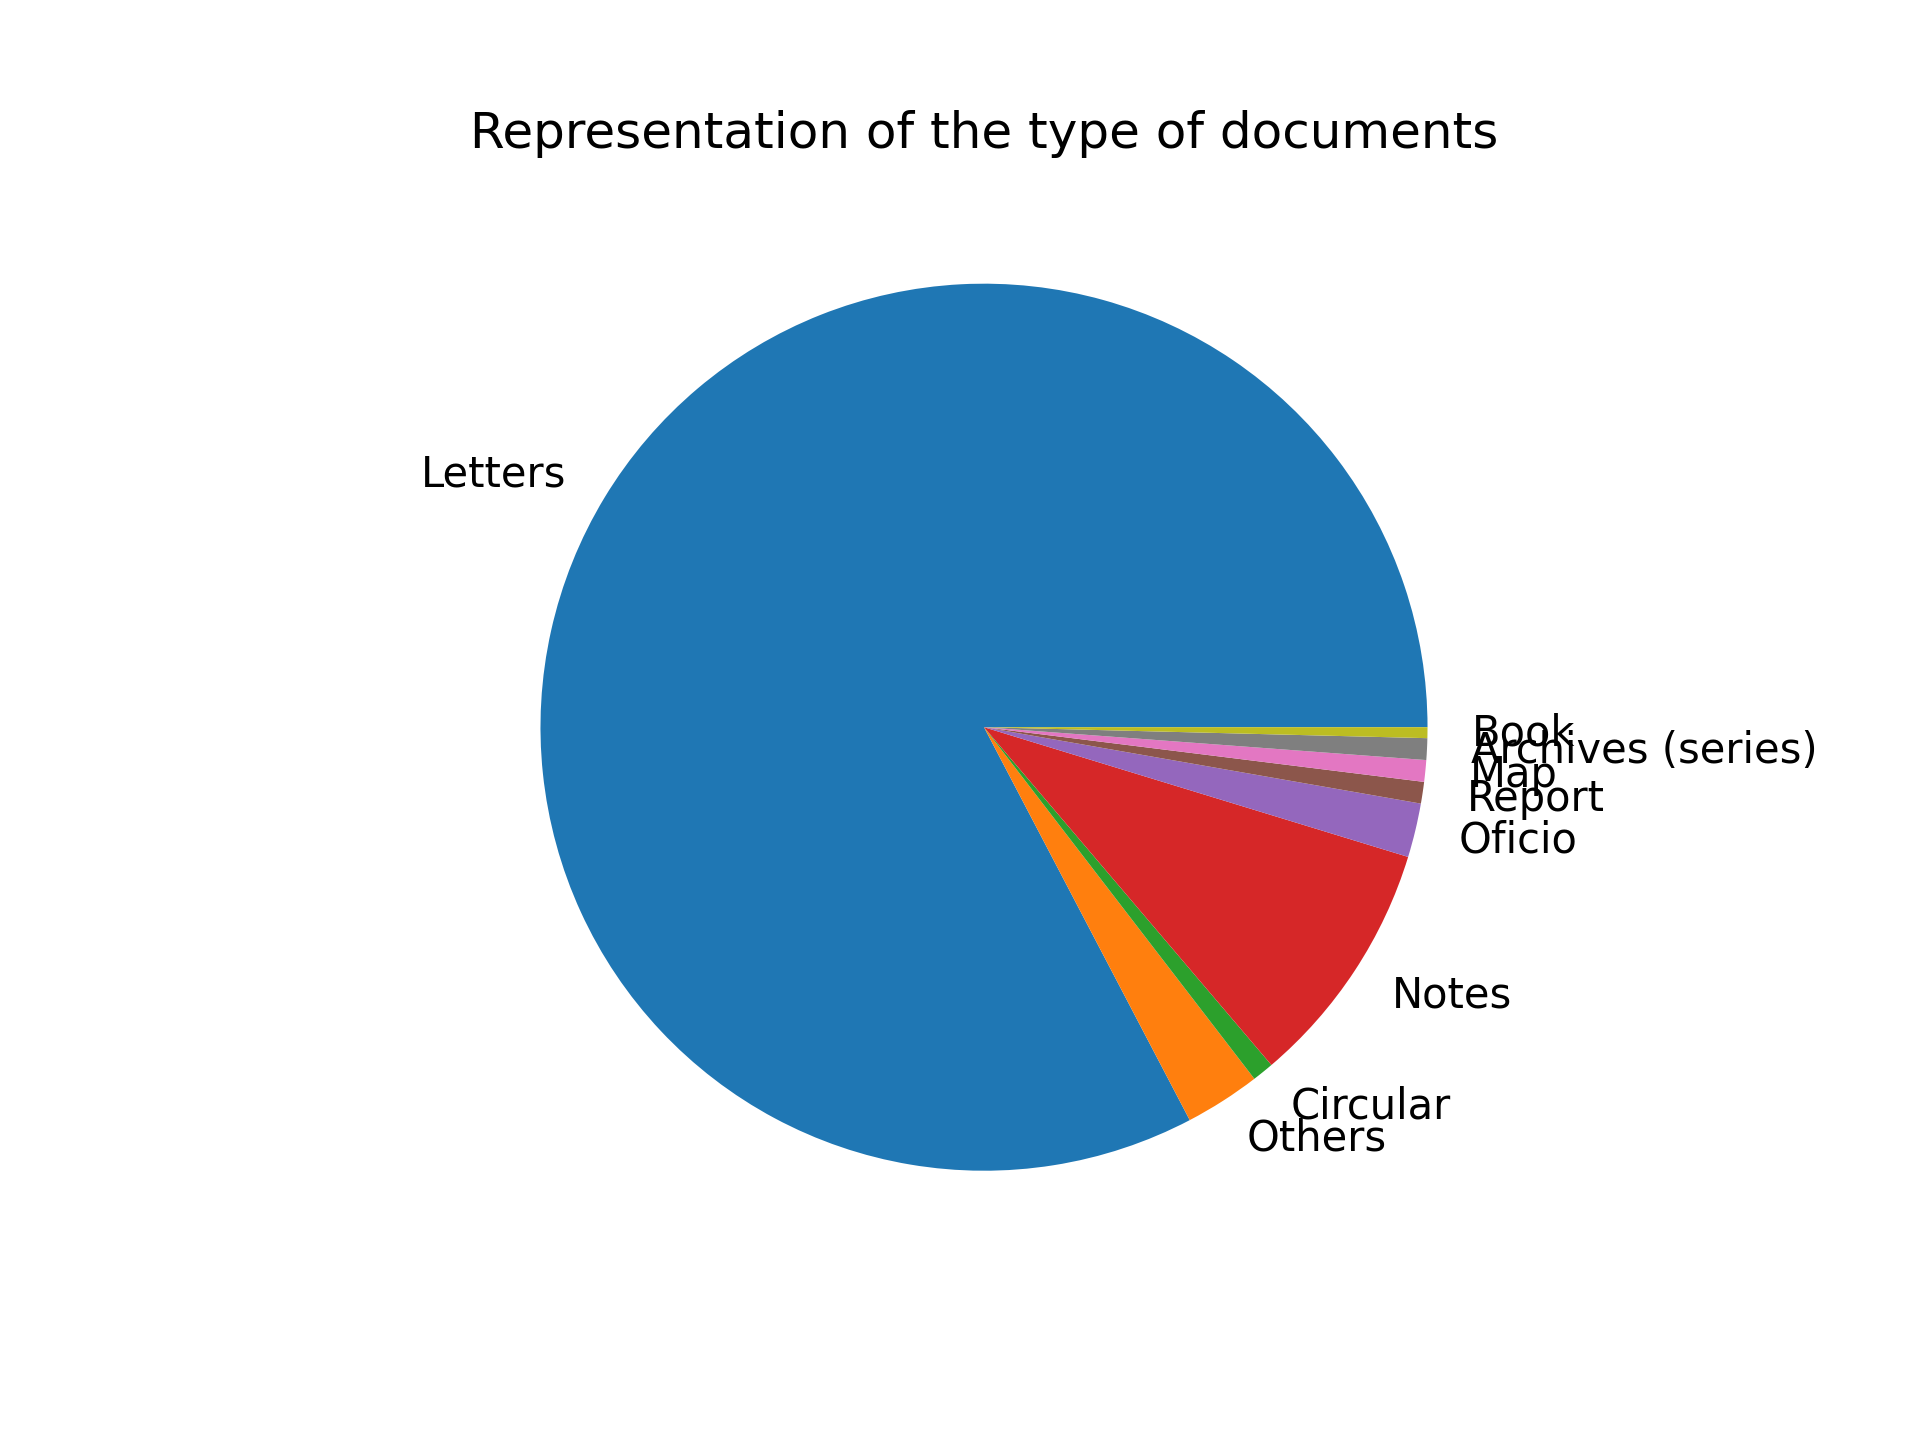
\includegraphics[width = 0.9\textwidth]{annexes/graph/percent_type.png}
    	\caption{Représentation des documents selon leur nature}
    	\label{fig:percent_type}
\end{figure}
\begin{figure}
    \centering
    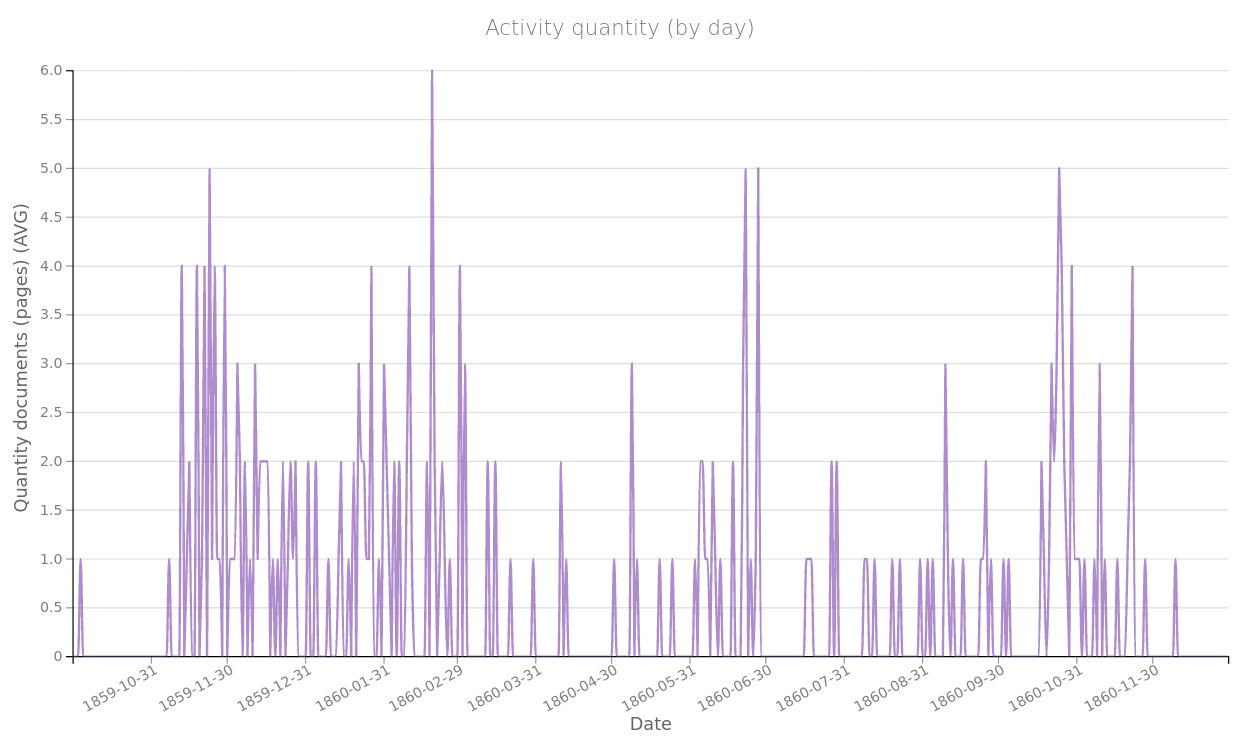
\includegraphics[width = 1\textwidth]{annexes/graph/activity_quantity_day.png}
    \caption{Activités documentaires sur les années 1859-1860 (par jours)}
    \label{fig:day_activities}
    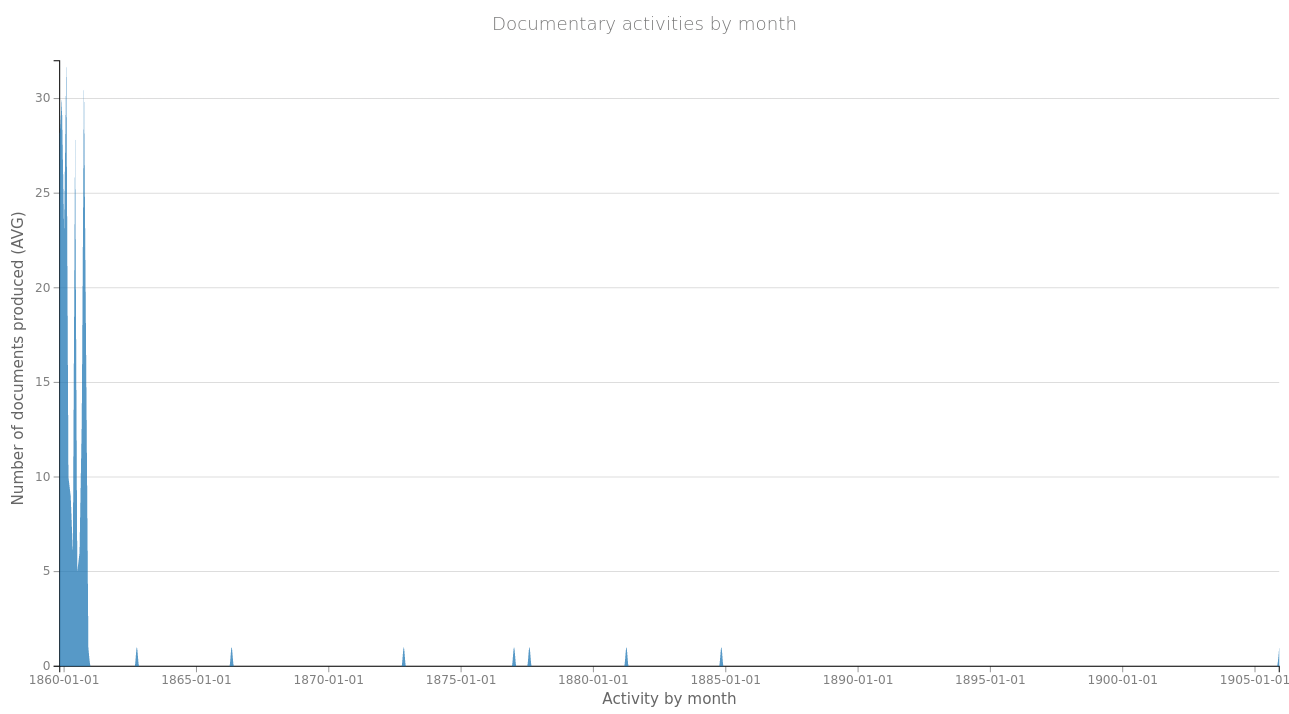
\includegraphics[width = 1\textwidth]{annexes/graph/archives_activity_month.png}
    \caption{Activités documentaires (par mois)}
    \label{fig:month_activities}
\end{figure}

\begin{figure}
     \centering
     \begin{subfigure}[b]{0.8\textwidth}
         \centering
         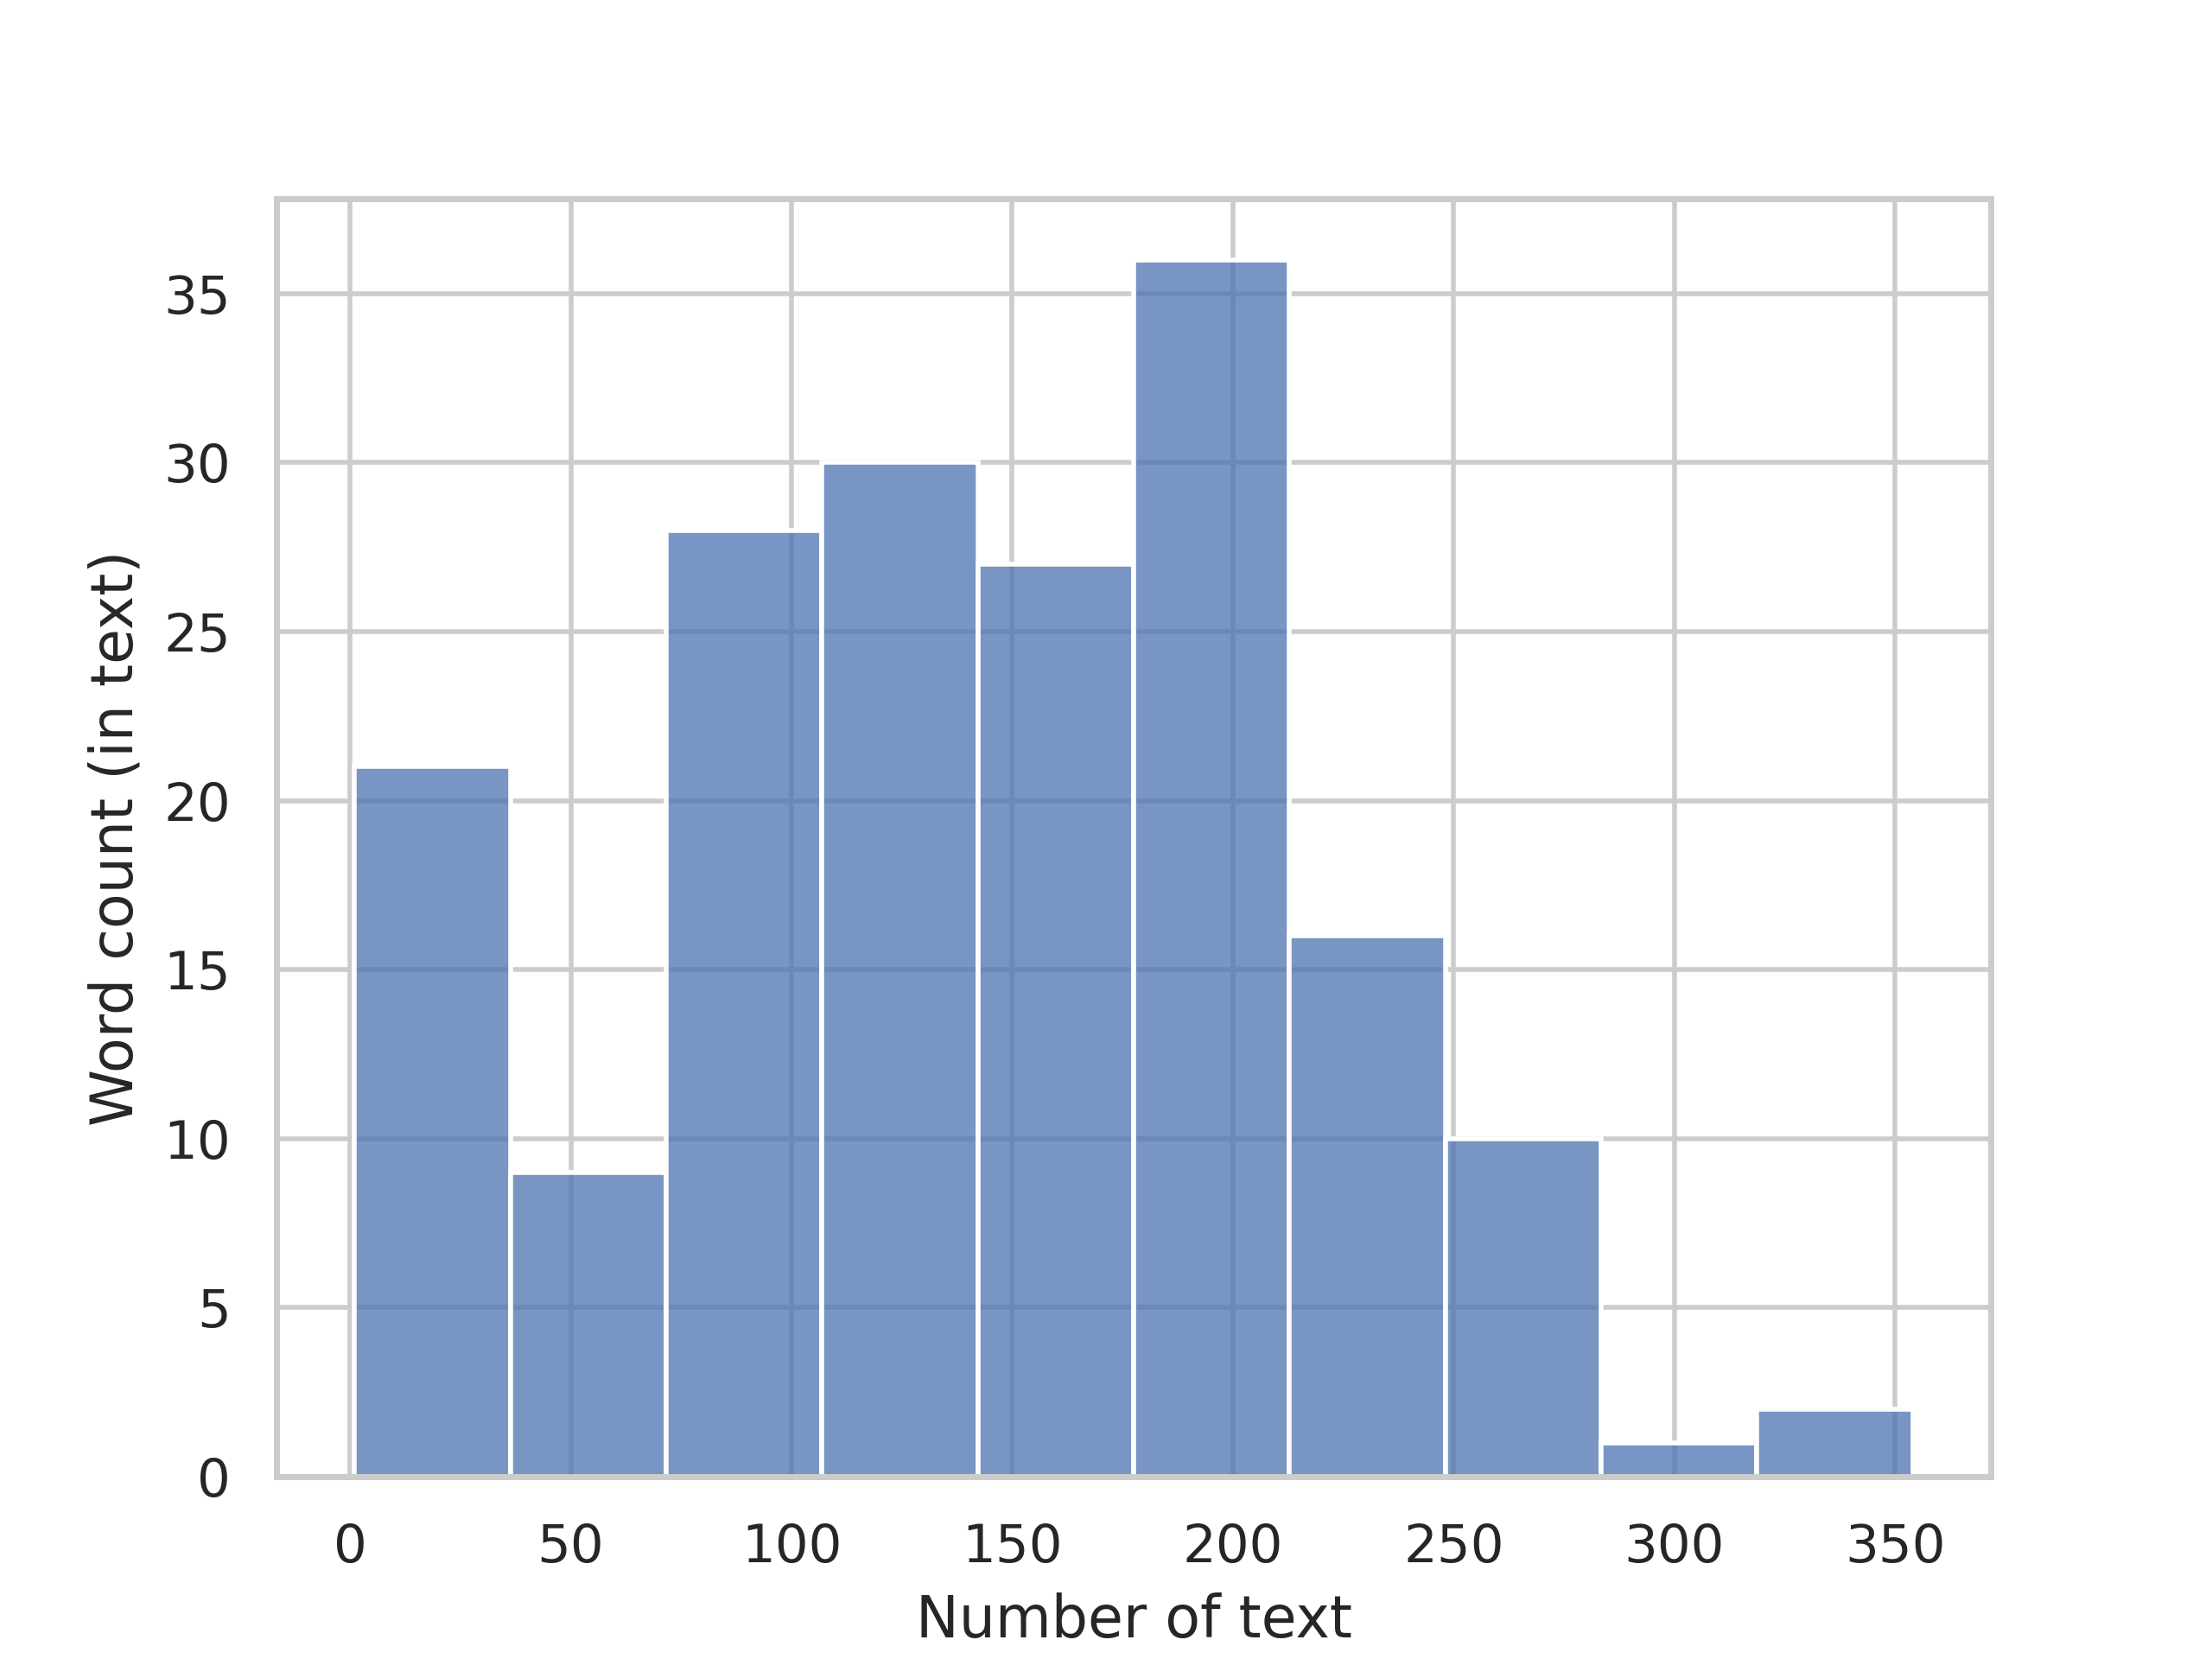
\includegraphics[width=\textwidth]{annexes/graph/histo_word_total.png}
         \caption{Par pages}
         \label{fig:histo_word_total}
     \end{subfigure}
     \hfill
     \begin{subfigure}[b]{0.8\textwidth}
         \centering
         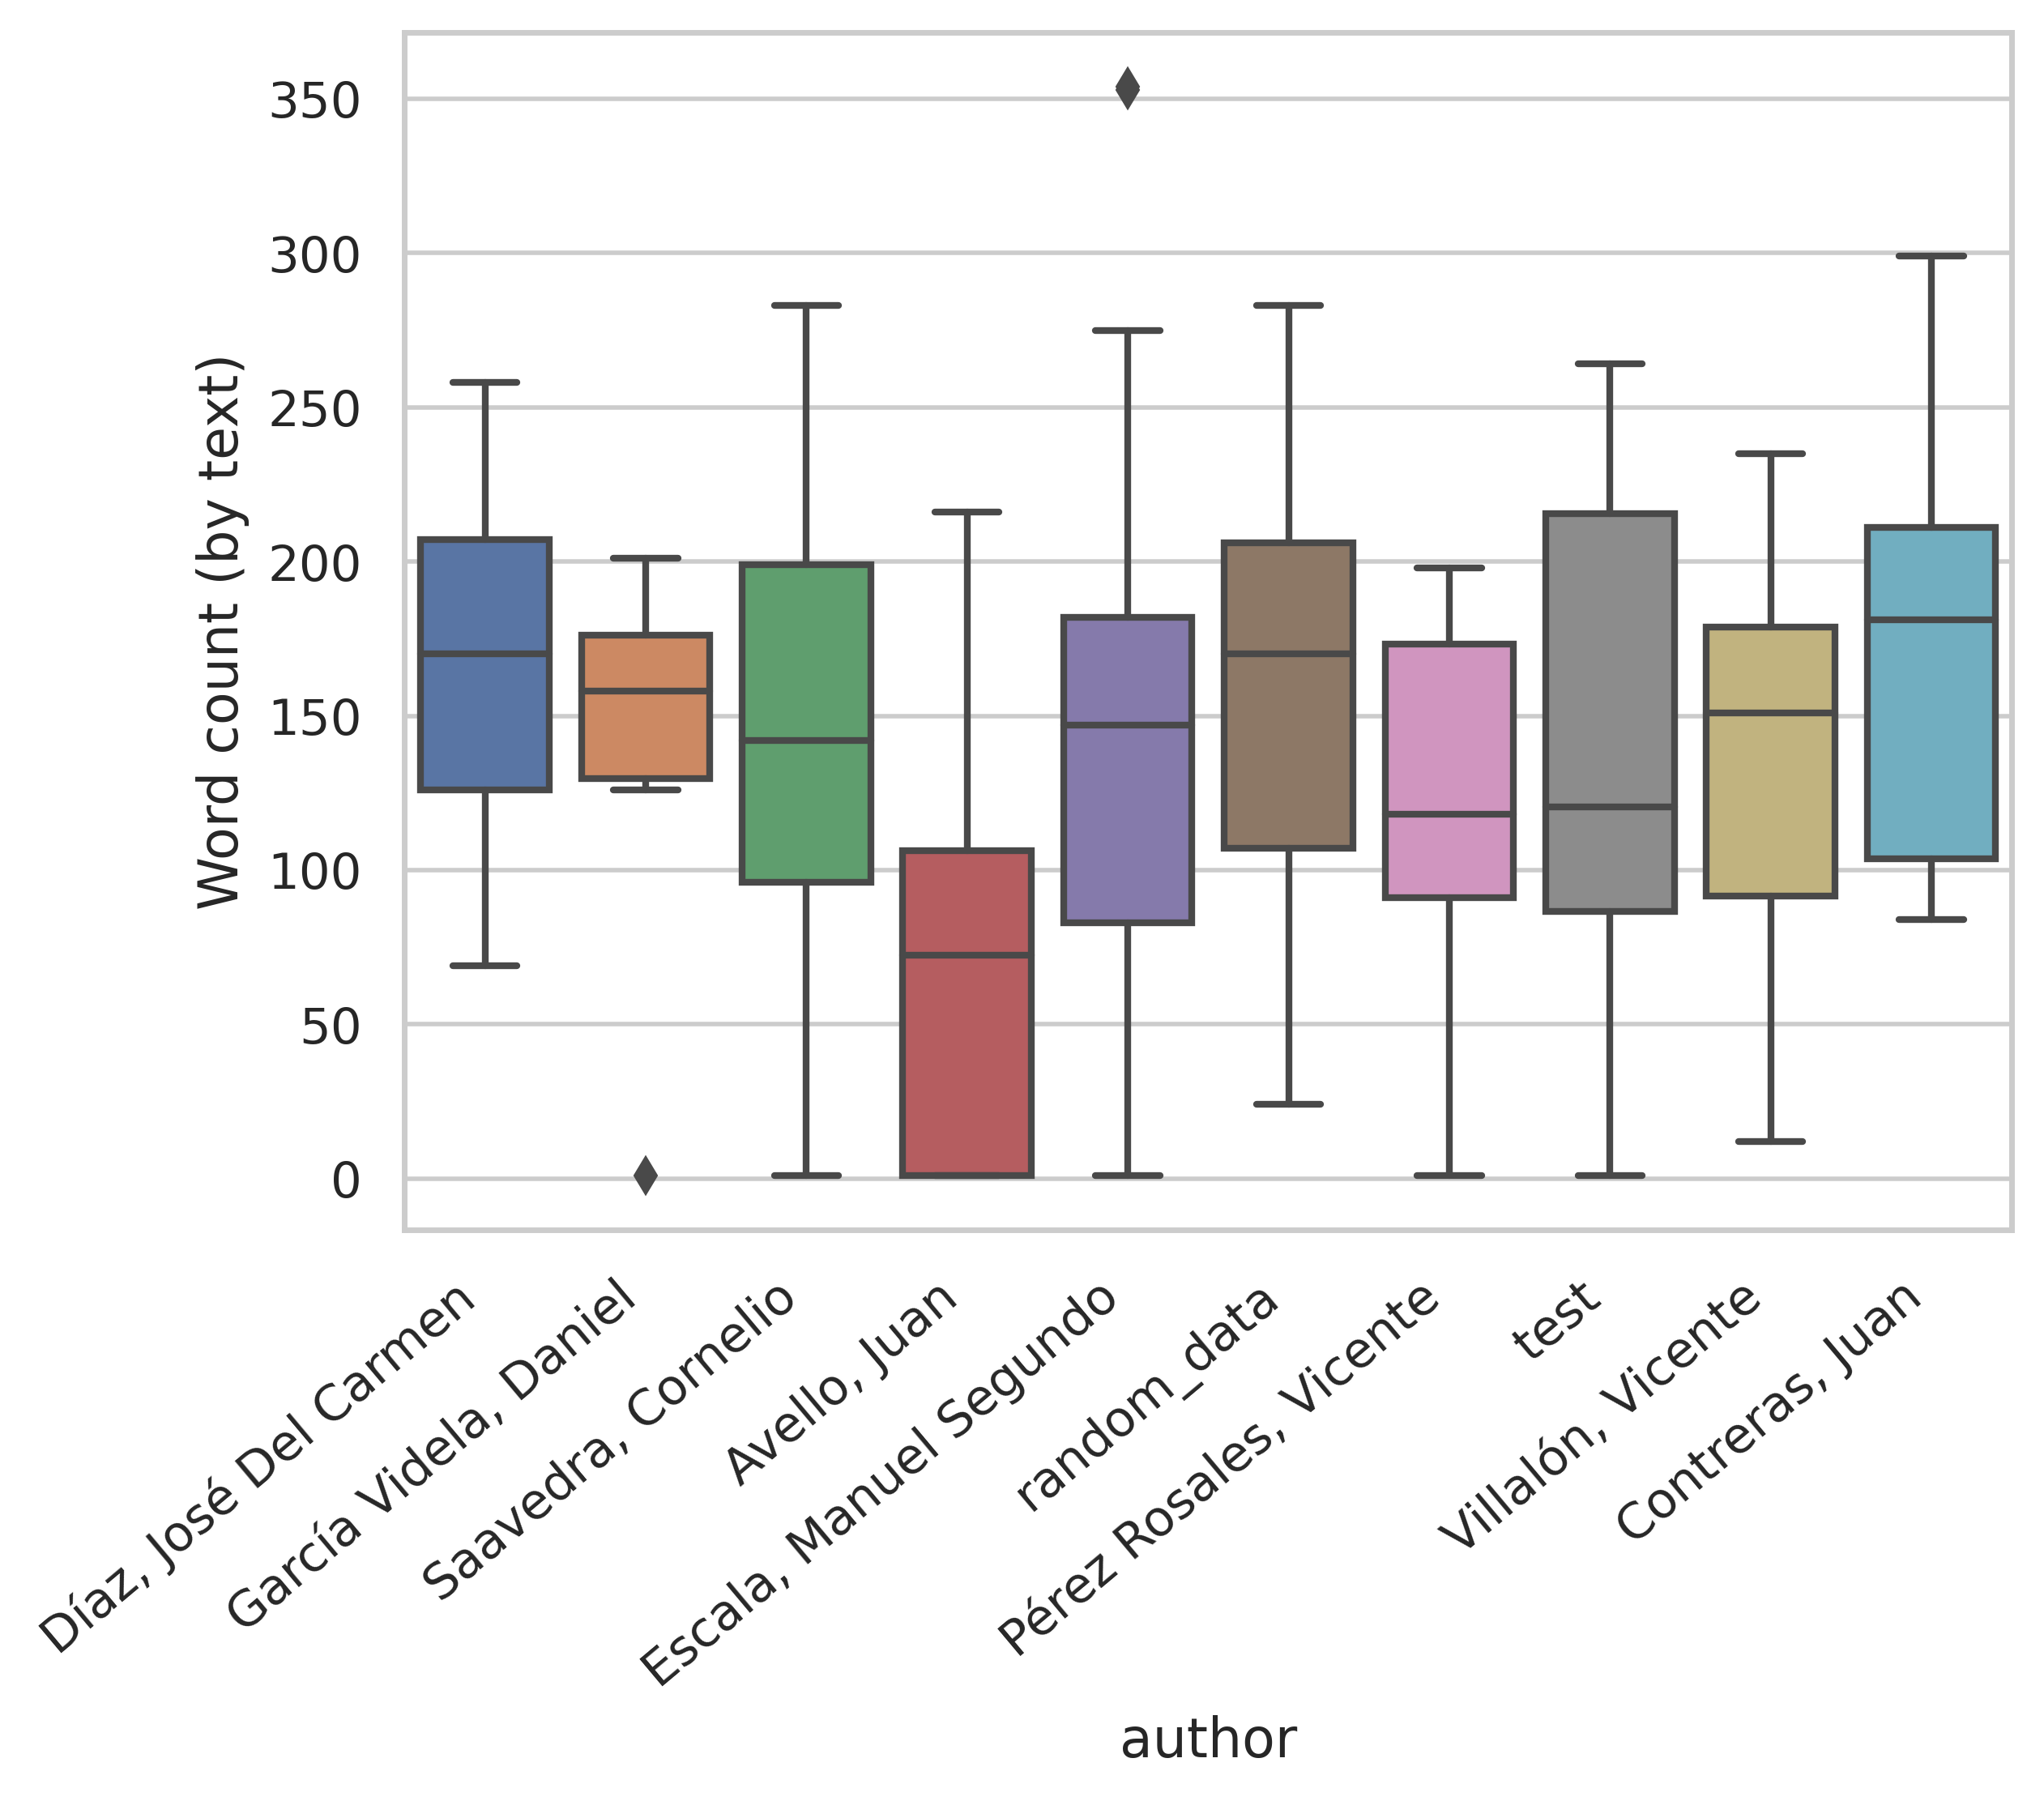
\includegraphics[width=\textwidth]{annexes/graph/boxtop_word.png}
         \caption{Par auteurs}
         \label{fig:boxtop_word}
     \end{subfigure}
     \caption{Distribution des mots}
    \label{fig:three graphs}
\end{figure}

\chapter{Automatisation d'une conversion de format d'image}
\chaptermark{Conversion de format d'image}
\begin{listing}
	        \begin{minted}{shell}
	        #!/bin/bash

                FOLDER=~/Bureau/data/jpg 
                ERROR="$FOLDER/error.txt"
                
                if ! [[ -d "$FOLDER" ]]|| ! [[ -e $ERROR ]]
                then
                	mkdir -p $FOLDER
                	touch $ERROR
                else
                    rm -f "$FOLDER/*.jpg"
                fi
                
                for img in "$PWD"/*.tif; do 
                    filename="$(basename "${img%.tif}")"
                    convert "$img" "$FOLDER/$filename.jpg"
                done 2>> $ERROR
	        \end{minted}
        	\caption{Script de conversion d'images TIFF vers le format JPG}
        	\label{code:shell_img}
\end{listing}

\chapter{Exemple de binarisation et de seuillage d'une image}
\chaptermark{}
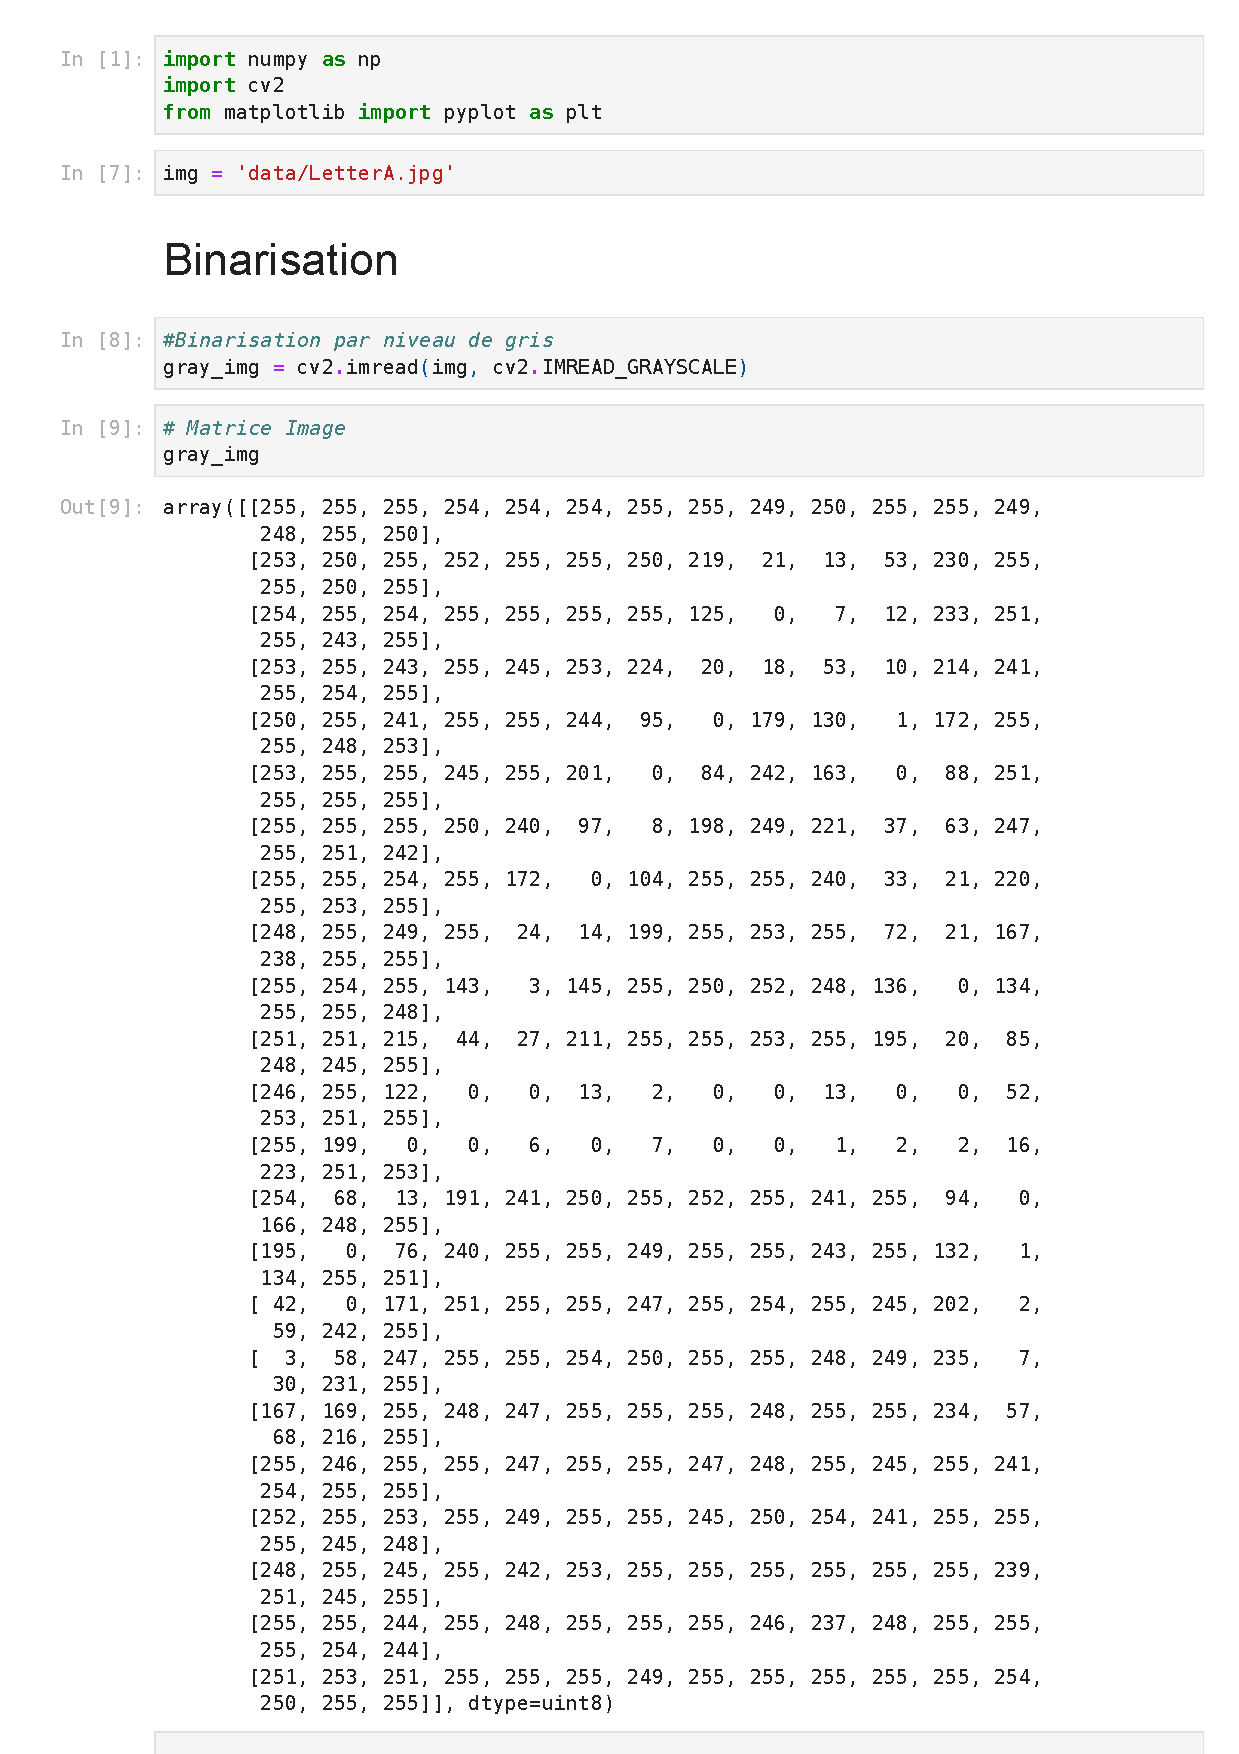
\includepdf[pages=-, pagecommand={}\label{code:traitement_image}]{annexes/pdf/traitement_image_HTR.pdf}

\chapter{Entraînement d'un modèle HTR avec Kraken}

\begin{listing}[h]
\centering
	        \begin{minted}{shell}
	        ketos train --augment --workers 8 -d cuda:0 -f binary --min-epochs 20 -w 0 -s '[1,120,0,1Cr3,13,32 Do0.1,2 Mp2,2 Cr3,13,32 Do0.1,2 Mp2,2 Cr3,9,64 Do0.1,2 Mp2,2 Cr3,9,64 Do0.1,2 S1(1x0)1,3 Lbx200 Do0.1,2 Lbx200 Do.1,2 Lbx200 Do]' --optimizer Adam -B 20 -r 0.0001 dataset.arrow > train_skratch.txt
	        \end{minted}
        	\caption{Commande shell d'entraînement selon la méthode \textit{skratch}}
        	\label{code:skratch}
\end{listing}

\begin{listing}[h]
    \centering
	        \begin{minted}{shell}
	        ketos train -f binary --augment -B 20 -d cuda:0 -o araucania_finetuning_McFrench --resize both --load HTR-United-Manu_McFrench.mlmodel dataset.arrow --lrate 0.0001 --workers 8 > train_finetuning.txt
	        \end{minted}
        	\caption{Commande shell d'entraînement selon la méthode \textit{finetuning}}
        	\label{code:finetuning}
\end{listing}

\begin{listing}[h]
            \centering
	        \begin{minted}{shell}
	        ketos segtrain --augment -d cuda:0 -s '[1,1800,0,3 Cr7,7,64,2,2 Gn32 Cr3,3,128,2,2 Gn32 Cr3,3,128 Gn32 Cr3,3,256 Gn32 Cr3,3,256 Gn32 Lbx32 Lby32 Cr1,1,32 Gn32 Lby32 Lbx32]' -f alto -bl data/**/*.xml -r 0.0001 --resize both --optimizer Adam -i models/blla.mlmodel --merge-baselines DefaultLine:default --merge-regions MainZone:text > segtrain.txt  
	        \end{minted}
        	\caption{Commande shell d'entraînement selon la méthode \textit{finetuning} d'un modèle de segmentation}
        	\label{code:segment}
\end{listing}

\chapter{Exemple de fichier XML-TEI : AH0299}
\chaptermark{Exemple de fichier XML-TEI}

\begin{minted}{xml}
<?xml version='1.0' encoding='UTF-8'?>
<TEI xmlns="http://www.tei-c.org/ns/1.0">
  <teiHeader>
    <fileDesc>
      <titleStmt>
        <title>Carta del 10 de junio de 1860 de Cornelio Saavedra a Mauricio Barbosa</title>
        <author>Saavedra, Cornelio</author>
        <editor>
          <orgName>Archivo Central Andres Bello</orgName>
        </editor>
      </titleStmt>
      <editionStmt>
        <respStmt>
          <resp xml:id="DirSc">Scientific Director of the edition</resp>
          <persName>
            <forename>Alessandro</forename>
            <surname>Chiaretti</surname>
            <roleName>Professor and archivist, responsable Área de Información Bibliográfica y Archivística</roleName>
            <affiliation>Archivo Central Andres Bello | Universidad de Chile</affiliation>
          </persName>
        </respStmt>
        <respStmt>
          <resp xml:id="Enc">In charge of digital encoding</resp>
          <persName>
            <forename>Maxime</forename>
            <surname>Humeau</surname>
            <roleName>Student, trainee</roleName>
            <affiliation>Ecole nationale des chartes | PSL</affiliation>
          </persName>
        </respStmt>
      </editionStmt>
      <extent>
        <measure unit="images" n="2"/>
      </extent>
      <publicationStmt>
        <publisher xml:id="ACAB">Archivo Central Andres Bello</publisher>
        <authority>Área de Información Bibliográfica y Archivística</authority>
        <address>
          <country key="CL"/>
          <region>Región Metropolitana</region>
          <settlement type="city">Santiago Centro</settlement>
          <postCode>8320000</postCode>
          <street>Arturo Prat</street>
          <street>#23</street>
        </address>
        <availability status="restricted">
          <licence target="https://creativecommons.org/licenses/by-sa/3.0/deed.fr">Attribution-NonCommercial-ShareAlike 4.0 International (CC BY-NC-SA 4.0)</licence>
          <p>Share — copy and redistribute the material in any medium or format</p>
          <p>Adapt — remix, transform, and build upon the material</p>
          <p>Attribution — You must give appropriate credit, provide a link to the license, and indicate if changes were made. You may do so in any reasonable manner, but not in any way that suggests the licensor endorses you or your use.</p>
          <p>NonCommercial — You may not use the material for commercial purposes.</p>
          <p>ShareAlike — If you remix, transform, or build upon the material, you must distribute your contributions under the same license as the original.</p>
          <p>The license is restricted to the use of XML-TEI files. The exploitation, distribution or publication of the attached images is subject to the approval of the institution. The full rights of the archive are reserved. The request can be made to the following address: &lt;email&gt;archivo.central@uchile.cl&lt;/email&gt;</p>
        </availability>
        <date when-iso="2022-08-15"/>
      </publicationStmt>
      <notesStmt>
        <note>Digital editing done as part of an international internship.</note>
        <note>A first transcription of part of the collection was made in &lt;date when-iso="2014-06"&gt;2014&lt;/date&gt; by &lt;persName&gt;Cecilia del Carmen Ramallo Díaz&lt;/persName&gt;.</note>
        <note>HTR scanning done at Universidad de Chile with kraken engine and the application eScriptorium. The HTR models from the transcript are available at this address &lt;ref target="https://github.com/Proyecto-Ocupacion-Araucania-UChile/model-HTR"&gt;github&lt;/ref&gt;</note>
      </notesStmt>
      <sourceDesc>
        <bibl>
          <series xml:lang="es">
            <title series="s" type="principal">Colección Manuscritos</title>
            <title type="subtitle">Pacificacion de la Araucania</title>
            <respStmt>
              <resp>Classification and conservation by</resp>
              <persName ref="#DirSc">Alessandro Chiaretti</persName>
              <persName xml:id="M_Parra">Marcos Parra</persName>
              <orgName ref="#ACAB">Área de Información Bibliográfica y Archivística</orgName>
            </respStmt>
            <idno type="caja" n="3"/>
            <idno type="id" n="AH0299"/>
            <note>
              <unit type="documents" quantity="255"/>
            </note>
          </series>
        </bibl>
      </sourceDesc>
    </fileDesc>
    <profileDesc>
      <particDesc>
        <listOrg>
          <head>List of organizations</head>
            <org xml:id="ORG_16832"><orgname>Gob^otu</orgname></org>
            <org xml:id="ORG_84978"><orgname>tropa</orgname></org>
            <org xml:id="ORG_89363"><orgname>cuerpo</orgname></org>
            <org xml:id="ORG_56624"><orgname>Co-misaría</orgname></org>
            <org xml:id="ORG_84978"><orgname>tropa</orgname></org>
            <org xml:id="ORG_74844"><orgname>Gobierno de Chile</orgname></org>
            <org xml:id="ORG_96712"><orgname>división</orgname></org>
        </listOrg>
        <listPerson>
          <head>List of persons</head>
            <person xml:id="PERS_41113" xml:base="N.C." xml:lang="es" sex="0"><persname>Mauricio Barbosa</persname></person>
            <person xml:id="PERS_86612" xml:base="N.C." xml:lang="es" sex="0"><persname>General</persname></person>
            <person xml:id="PERS_70914" xml:base="N.C." xml:lang="es" sex="0"><persname>doctor</persname></person>
            <person xml:id="Q1327" xml:base="https://viaf.org/viaf/26785781" xml:lang="en" sex="1.0"><persname>José Joaquín Pérez</persname><birth when-iso="1801-05-06">6 de mayo de 1801</birth><death when-iso="1889-07-01">1 de julio de 1889</death><note type="description">Chilean politician and President (1801-1889)</note></person>
            <person xml:id="PERS_46502" xml:base="N.C." xml:lang="es" sex="0"><persname>Ocha-gavía</persname></person>
            <person xml:id="Q5945826" xml:base="https://viaf.org/viaf/50032889" xml:lang="en" sex="1.0"><persname>José Tomás Urmeneta</persname><birth when-iso="1808-10-08">8 de octubre de 1808</birth><death when-iso="1878-10-20">20 de octubre de 1878</death><note type="description">Chilean politician</note></person>
            <person xml:id="PERS_47745" xml:base="N.C." xml:lang="es" sex="0"><persname>Boonen</persname></person><person xml:id="Q4233309" xml:base="https://viaf.org/viaf/5,34145858091523E+020" xml:lang="en" sex="1.0"><persname>Cornelio Saavedra Rodríguez</persname><birth when-iso="1821-01-01">1 de enero de 1821</birth><death when-iso="1891-04-07">7 de abril de 1891</death><note type="description">Chilean general</note></person>
        </listPerson>
      </particDesc>
      <settingDesc>
        <listPlace>
          <head>List of places</head>
        <place xml:id="Q33986" xml:base="https://www.geonames.org/3868626" xml:lang="en" type="city_in_Chile"><placename>Valparaíso</placename><region>Valparaíso</region><country>Chile</country><geo>-71.619722222 -33.046111111</geo><note type="description">city in Chile</note></place>
        <place xml:id="LOC_88528" xml:base="N.C." xml:lang="es" type="None"><placename>Tucapel</placename></place><place xml:id="LOC_18849" xml:base="N.C." xml:lang="es" type="None"><placename>Los Angeles</placename></place>
        <place xml:id="Q3632" xml:base="https://www.geonames.org/3899462" xml:lang="en" type="city_in_Chile"><placename>Arauco</placename><region>Arauco</region><country>Chile</country><geo>-73.3175 -37.2463</geo><note type="description">Chilean commune</note></place>
        </listPlace>
      </settingDesc>
    </profileDesc>
    <encodingDesc>
      <editorialDecl>
        <p>Encoding with XML-TEI P5</p>
        <correction>
          <p>There are no corrections for spelling or grammatical errors. The transcription is as original as possible. A post-process HTR correction was performed via spellchecker and Levenshtein's Distance algorithm.</p>
        </correction>
        <punctuation>
          <p>The punctuation has been transcribed as found.</p>
        </punctuation>
        <segmentation target="https://github.com/segmonto">
          <p>The segmentation is done via the kraken segmentation model and restructured from the XML-ALTO files and Segmonto ontology.</p>
        </segmentation>
        <normalization>
          <p>Words that are crossed out, illegible or only interpretable have not been transcribed.</p>
        </normalization>
      </editorialDecl>
      <appInfo>
        <application version="4.1.1" ident="kraken">
          <label>Kraken HTR</label>
          <ptr target="https://github.com/mittagessen/kraken"/>
        </application>
        <application version="1.0.0" ident="escriptorium">
          <label>eScriptorium</label>
          <ptr target="https://gitlab.com/scripta/escriptorium"/>
        </application>
        <application version="0.6.3" ident="pyspellchecker">
          <label>PYspellchecker</label>
          <ptr target="https://github.com/barrust/pyspellchecker"/>
        </application>
        <application version="3.4" ident="spacy">
          <label>spaCy</label>
          <ptr target="https://github.com/explosion/spaCy"/>
        </application>
      </appInfo>
    </encodingDesc>
  </teiHeader>
  <sourceDoc>
  [...]
  </sourceDoc>
  <text>
    <body>
      <div type="Letters">
        <pb corresp="#299_a"/>
        <opener>
          <dateline corresp="#299_a_z1"><placename resp="spacy" ref="#Q33986"><lb corresp="#299_a_z1_l1"/>Valparaiso</placename>, <date resp="spacy">Julio 101860</date></dateline>
          <dateline corresp="#299_a_z1"><placename resp="spacy" ref="#LOC_88528"><lb corresp="#299_a_z1_l2"/>Tucapel</placename></dateline>
          <name corresp="#299_a_z2" type="addressee"><lb corresp="#299_a_z2_l1"/>Sr D. <persname resp="spacy" ref="#PERS_41113">Mauricio Barboza</persname></name>
          <salute corresp="#299_a_z4"><lb corresp="#299_a_z4_l1"/>Mi estimado amigo:</salute>
        </opener>
        <p corresp="#299_a_z3" n="1"><lb corresp="#299_a_z3_l1"/>Tus cartas del <date resp="spacy">17 de Junio</date> son las únicas que<lb corresp="#299_a_z3_l2"/>he recibido desde que fuiste a <placename resp="spacy" ref="#LOC_18849">Los Angeles</placename> y con tanto atraso han llega-<lb corresp="#299_a_z3_l3"/>do a mi poder que hacen solo <date resp="spacy">dos días</date> las he recibido y en el mo-<lb corresp="#299_a_z3_l4"/>mento he tomado medidas para alistar un buque y avisar al <orgname resp="spacy" ref="#ORG_16832">Gob^o<lb corresp="#299_a_z3_l5"/>tu</orgname> situacion. <date resp="spacy">Hoi</date> se ordena ya la salida del “Maule” y embarque de<lb corresp="#299_a_z3_l6"/>víveres y el <date resp="spacy">viernes 13</date> estará de viaje este vapor para proporcionarte<lb corresp="#299_a_z3_l7"/>los auxilios necesarios.</p>
        <p corresp="#299_a_z3" n="2"><lb corresp="#299_a_z3_l8"/>Los techos están listos para mandartelos cuando tu creas<lb corresp="#299_a_z3_l9"/>convenientes emprender el trabajo y tengas los elementos necesa-<lb corresp="#299_a_z3_l10"/>rios para conducir el fierro. De todos modos te los había<lb corresp="#299_a_z3_l11"/>mandado por el Maule, pero este vapor es tan pequeño que<lb corresp="#299_a_z3_l12"/>apenas puede llevarte los víveres.</p>
        <p corresp="#299_a_z3" n="3"><lb corresp="#299_a_z3_l13"/>En cuanto a la remesa de artículos, te mando lo que<lb corresp="#299_a_z3_l14"/>creo puedas necesitar tanto para la <orgname resp="spacy" ref="#ORG_84978">tropa</orgname> como para los ofi-<lb corresp="#299_a_z3_l15"/>ciales y lo que no necesites, bien puedes realizarlo en esa con<lb corresp="#299_a_z3_l16"/>ventaja y evitar el cargo que irá contra tu <orgname resp="spacy" ref="#ORG_89363">cuerpo</orgname>. La <orgname resp="spacy" ref="#ORG_56624">Co-<lb corresp="#299_a_z3_l17"/>misaría</orgname> ha sido la encargada para esta compra.</p>
        <p corresp="#299_a_z3" n="4"><lb corresp="#299_a_z3_l18"/>Debes pues estar prevenido de la llegada del “Maule” y si<lb corresp="#299_a_z3_l19"/>encuentras mas prudente retirarte sobre <placename resp="spacy" ref="#Q3632">Arauco</placename>, debes hacerlo<lb corresp="#299_a_z3_l20"/>a pesar que sería nuevo sacrificio llevar tu <orgname resp="spacy" ref="#ORG_84978">tropa</orgname> a esa locali-<lb corresp="#299_a_z3_l21"/>dad pasado el invierno, el que estando ya mui adelantado<lb corresp="#299_a_z3_l22"/>hace desaparezca luego tu penosa situacion; sinembargo tu<lb corresp="#299_a_z3_l23"/>veras lo mas conveniente.</p>
        <p corresp="#299_a_z3" n="5"><lb corresp="#299_a_z3_l24"/>El <persname resp="spacy" ref="#PERS_86612">General</persname> me dice que te dirijas oficialmente al <orgname resp="spacy" ref="#ORG_74844">Gob^o</orgname></p>
        <pb corresp="#299_b"/>
        <p corresp="#299_b_z1" n="6"><lb corresp="#299_b_z1_l1"/>pidiendo las medicinas y médico que necesitas y ya tengo<lb corresp="#299_b_z1_l2"/>encargo de buscarte un <persname resp="spacy" ref="#PERS_70914">doctor</persname> para que esté con tu <orgname resp="spacy" ref="#ORG_96712">división</orgname>.</p>
        <p corresp="#299_b_z1" n="7"><lb corresp="#299_b_z1_l3"/>En cuanto al abono de real diario no será posible y te<lb corresp="#299_b_z1_l4"/>lo aviso para que procures la economía en el rancho de tropa.</p>
        <p corresp="#299_b_z1" n="8"><lb corresp="#299_b_z1_l5"/>Por acá no ocurre novedad ninguna que pueda co-<lb corresp="#299_b_z1_l6"/>municarte, todo sigue tranquilo y con mas que segurida-<lb corresp="#299_b_z1_l7"/>des que continuaremos del mismo modo.</p>
        <p corresp="#299_b_z1" n="9"><lb corresp="#299_b_z1_l8"/>En materia de política hai mucho silencio y en cuanto<lb corresp="#299_b_z1_l9"/>a candidatos se habla de Don <persname resp="spacy" ref="#Q1327">José Joaquín Pérez</persname>, <persname resp="spacy" ref="#PERS_46502">Ocha-<lb corresp="#299_b_z1_l10"/>gavía</persname> y Don <persname resp="spacy" ref="#Q5945826">José Tomás Urmeneta</persname>, mas probablemente<lb corresp="#299_b_z1_l11"/>se fijará la atención sobre los dos primeros: todavia esto<lb corresp="#299_b_z1_l12"/>es un problema que se decidirá en pocos meses mas.</p>
        <p corresp="#299_b_z1" n="10"><persname resp="spacy" ref="#PERS_47745"><lb corresp="#299_b_z1_l13"/>Boonen</persname> recibió el recibo que me mandaste y me dice<lb corresp="#299_b_z1_l14"/>que tiene en su poder $ 300 poco mas ó menos de los que<lb corresp="#299_b_z1_l15"/>te dará cuenta o pondrá a tu disposicion.</p>
        <fw corresp="#299_b_z2" type="n_page"><lb corresp="#299_b_z2_l1"/>2</fw>
        <closer>
          <signed><persname resp="spacy" ref="#Q4233309"><lb corresp="#299_b_z4_l1"/>Cornelio Saavedra</persname></signed>
          <salute corresp="#299_b_z5" n="11"><lb corresp="#299_b_z5_l1"/>Como siempre me repito tu amigo y S.S.</salute>
        </closer>
      </div>
    </body>
    <noteGrp>
      <note corresp="#299_b_z3_l1" type="id_imp">000299</note>
    </noteGrp>
  </text>
  </TEI>
\end{minted}

\chapter{Résultats des évaluation NER par \textit{cross-validation}}
\chaptermark{Résultats des évaluation NER}

\begin{minted}{json}
[
    {
      "token_acc":1.0,
      "token_p":1.0,
      "token_r":1.0,
      "token_f":1.0,
      "ents_p":0.7134831461,
      "ents_r":0.7298850575,
      "ents_f":0.7215909091,
      "ents_per_type":{
        "MISC":{
          "p":0.7647058824,
          "r":0.4333333333,
          "f":0.5531914894
        },
        "LOC":{
          "p":0.7777777778,
          "r":0.875,
          "f":0.8235294118
        },
        "DATE":{
          "p":0.52,
          "r":0.7647058824,
          "f":0.619047619
        },
        "PERS":{
          "p":0.75,
          "r":0.7611940299,
          "f":0.7555555556
        },
        "ORG":{
          "p":0.6875,
          "r":0.7857142857,
          "f":0.7333333333
        }
      },
      "speed":2742.5599353071
    },
    {
      "token_acc":1.0,
      "token_p":1.0,
      "token_r":1.0,
      "token_f":1.0,
      "ents_p":0.7556818182,
      "ents_r":0.7643678161,
      "ents_f":0.76,
      "ents_per_type":{
        "MISC":{
          "p":0.5517241379,
          "r":0.5333333333,
          "f":0.5423728814
        },
        "LOC":{
          "p":0.9,
          "r":0.84375,
          "f":0.8709677419
        },
        "DATE":{
          "p":0.8125,
          "r":0.7647058824,
          "f":0.7878787879
        },
        "PERS":{
          "p":0.7746478873,
          "r":0.8208955224,
          "f":0.7971014493
        },
        "ORG":{
          "p":0.7333333333,
          "r":0.7857142857,
          "f":0.7586206897
        }
      },
      "speed":2522.5018865445
    },
    {
      "token_acc":1.0,
      "token_p":1.0,
      "token_r":1.0,
      "token_f":1.0,
      "ents_p":0.7,
      "ents_r":0.724137931,
      "ents_f":0.7118644068,
      "ents_per_type":{
        "MISC":{
          "p":0.6,
          "r":0.6,
          "f":0.6
        },
        "LOC":{
          "p":0.7878787879,
          "r":0.8125,
          "f":0.8
        },
        "DATE":{
          "p":0.6875,
          "r":0.6470588235,
          "f":0.6666666667
        },
        "PERS":{
          "p":0.6944444444,
          "r":0.7462686567,
          "f":0.7194244604
        },
        "ORG":{
          "p":0.724137931,
          "r":0.75,
          "f":0.7368421053
        }
      },
      "speed":2520.9481323492
    },
    {
      "token_acc":1.0,
      "token_p":1.0,
      "token_r":1.0,
      "token_f":1.0,
      "ents_p":0.7167630058,
      "ents_r":0.7126436782,
      "ents_f":0.7146974063,
      "ents_per_type":{
        "MISC":{
          "p":0.7083333333,
          "r":0.5666666667,
          "f":0.6296296296
        },
        "LOC":{
          "p":0.8333333333,
          "r":0.78125,
          "f":0.8064516129
        },
        "DATE":{
          "p":0.5416666667,
          "r":0.7647058824,
          "f":0.6341463415
        },
        "PERS":{
          "p":0.7868852459,
          "r":0.7164179104,
          "f":0.75
        },
        "ORG":{
          "p":0.6176470588,
          "r":0.75,
          "f":0.6774193548
        }
      },
      "speed":2756.2619204097
    },
    {
      "token_acc":1.0,
      "token_p":1.0,
      "token_r":1.0,
      "token_f":1.0,
      "ents_p":0.7045454545,
      "ents_r":0.7126436782,
      "ents_f":0.7085714286,
      "ents_per_type":{
        "MISC":{
          "p":0.6363636364,
          "r":0.4666666667,
          "f":0.5384615385
        },
        "LOC":{
          "p":0.7352941176,
          "r":0.78125,
          "f":0.7575757576
        },
        "DATE":{
          "p":0.7647058824,
          "r":0.7647058824,
          "f":0.7647058824
        },
        "PERS":{
          "p":0.7571428571,
          "r":0.7910447761,
          "f":0.7737226277
        },
        "ORG":{
          "p":0.5757575758,
          "r":0.6785714286,
          "f":0.6229508197
        }
      },
      "speed":2619.3018869685
    },
    {
      "token_acc":1.0,
      "token_p":1.0,
      "token_r":1.0,
      "token_f":1.0,
      "ents_p":0.7607361963,
      "ents_r":0.7126436782,
      "ents_f":0.7359050445,
      "ents_per_type":{
        "MISC":{
          "p":0.8823529412,
          "r":0.5,
          "f":0.6382978723
        },
        "LOC":{
          "p":0.8064516129,
          "r":0.78125,
          "f":0.7936507937
        },
        "DATE":{
          "p":0.8666666667,
          "r":0.7647058824,
          "f":0.8125
        },
        "PERS":{
          "p":0.7352941176,
          "r":0.7462686567,
          "f":0.7407407407
        },
        "ORG":{
          "p":0.65625,
          "r":0.75,
          "f":0.7
        }
      },
      "speed":2471.587894989
    }
]
\end{minted}

\chapter{Visualisation des modèles NER}

\begin{figure}
    \centering
    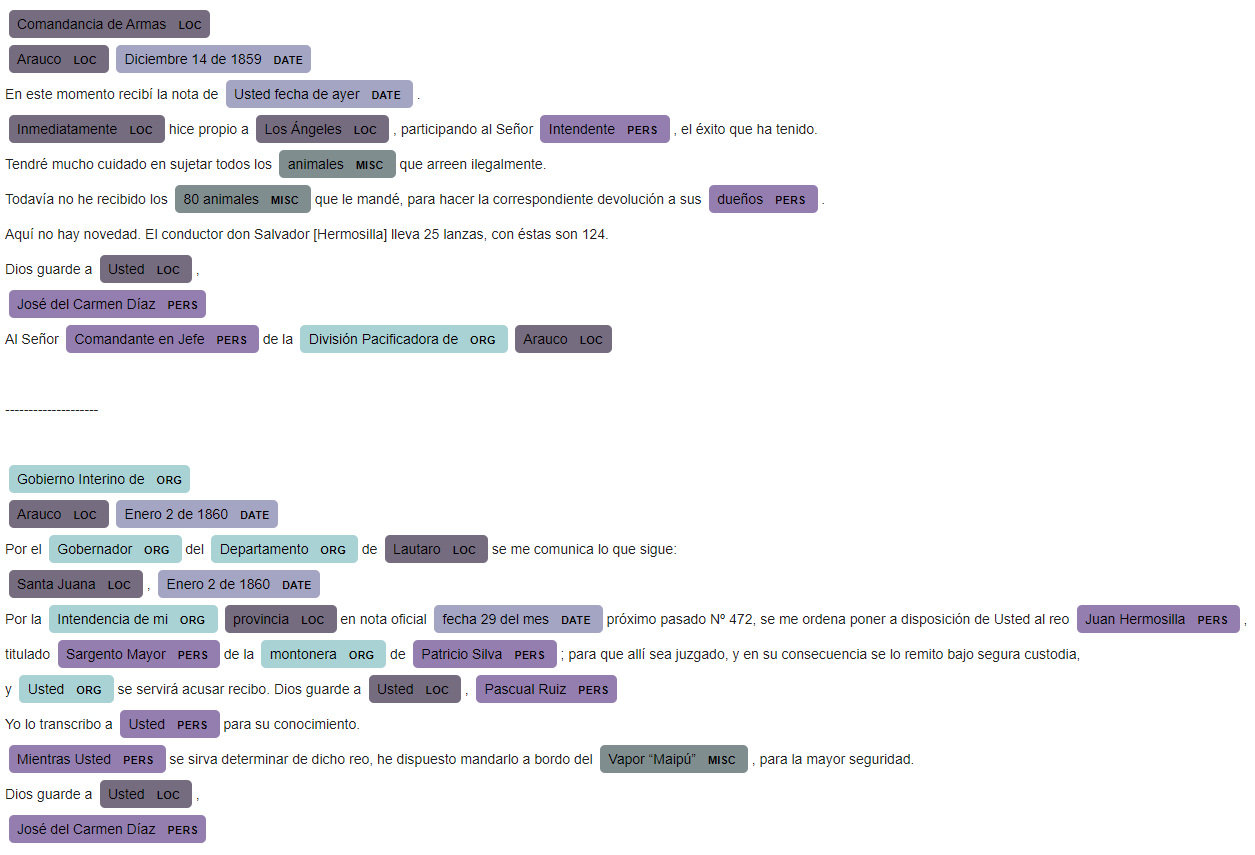
\includegraphics[width=0.8\textwidth]{annexes/img/k2_viz.png}
    \caption{Visualisation du modèle NER $\kappa_2$}
    \label{fig:k2_viz}
\end{figure}

\begin{figure}
    \centering
    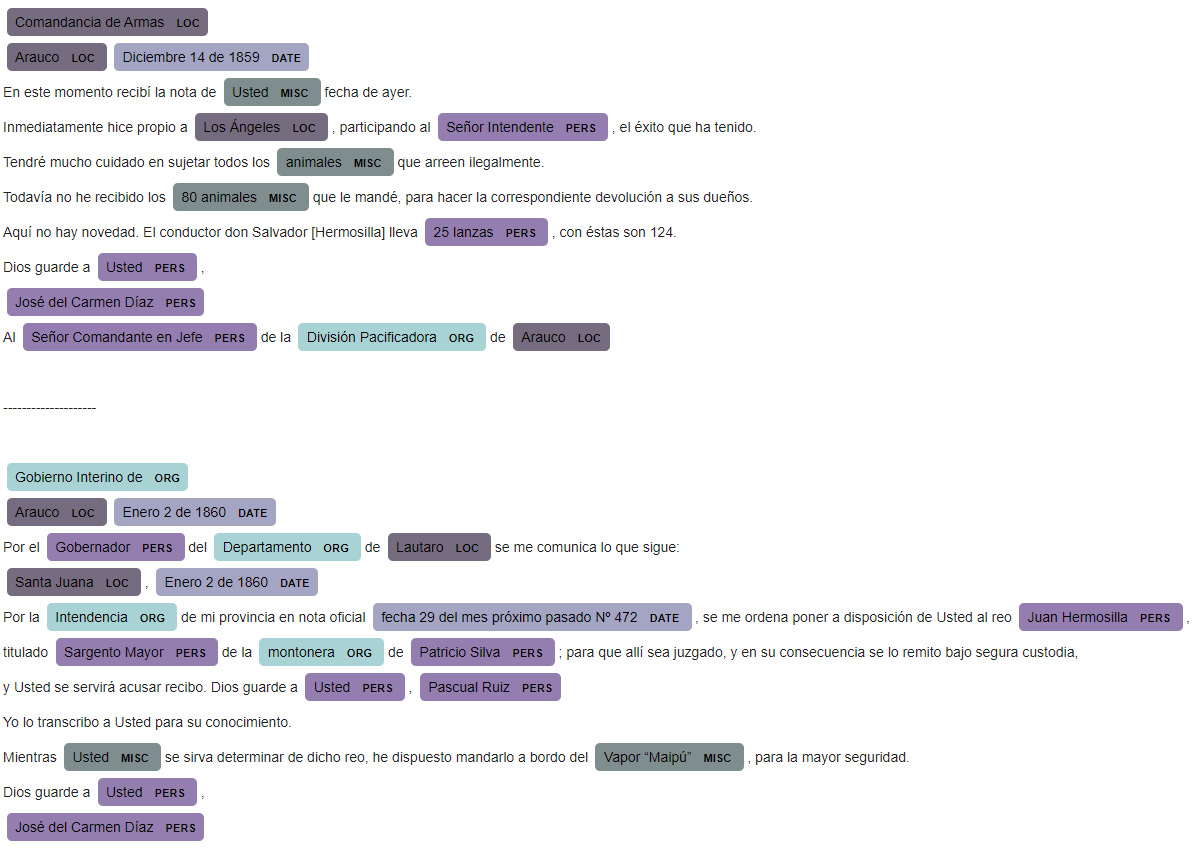
\includegraphics[width=0.8\textwidth]{annexes/img/k6_viz.png}
    \caption{Visualisation du modèle NER $\kappa_6$}
    \label{fig:k6_viz}
\end{figure}

\chapter{Modélisation d'entité XML-TEI à partir d'une requête SPARQL}
\chaptermark{Modélisation d'entité XML-TEI}

\begin{listing}[h]
	        \begin{minted}{xml}
<person xml:id="Q4233309" xml:base="https://viaf.org/viaf/534145858091523021888" xml:lang="en" sex="1.0">
  <persname>Cornelio Saavedra Rodríguez</persname>
  <birth when-iso="1821-01-01">1 de enero de 1821</birth>
  <death when-iso="1891-04-07">7 de abril de 1891</death>
  <note type="description">Chilean general</note>
</person>
	        \end{minted}
        	\caption{Structuration du <person> au sein du <particDesc>}
        	\label{code:ent_pers}
\end{listing}

\begin{listing}[h]
	        \begin{minted}{xml}
<place xml:id="Q33986" xml:base="https://www.geonames.org/3868626" xml:lang="en" type="city_in_Chile">
  <placename>Valparaíso</placename>
  <region>Valparaíso</region>
  <country>Chile</country>
  <geo>-71.619722222 -33.046111111</geo>
  <note type="description">city in Chile</note>
</place>
	        \end{minted}
        	\caption{Structuration du <place> au sein du <settingDesc>}
        	\label{code:ent_loc}
\end{listing}
	
	\backmatter

% figures & tables
	\listoffigures
	\listoftables
	\listoflistings

% table des matières
	\tableofcontents
	
\end{document}